% !TeX encoding = UTF-8 Unicode
% !TeX program = xelatex+makeindex+bibtex
% !TeX spellcheck = sk-SK
%
% \begin{english}
% This is a translation to Slovak language of the book Fundamentals of Piano Practice, 2nd ed. (c)2009 Chuan C. Chang
% Translation (c)2015 Ladislav Rado
%
% To compile this document to PDF use XeLaTeX, with these fonts installed:
% - Linux Libertine O
% - Emmentaler
% - TeX Gyre Schola Math
%
% Illustration of the piano on the front page is in the Public Domain.
% It has been taken from http://openclipart.org/detail/366/piano-by-theresaknott
% and converted from SVG format to PDF.
% \end{english}
%
% \begin{slovak}
% Základy cvičenia na klavíri
% ---------------------------
% Toto je preklad do slovenčiny knihy Fundamentals of Piano Practice, 2nd ed. (c)2009 Chuan C. Chang
% Preklad (c)2015 Ladislav Rado
%
% Na skompilovanie tohto dokumentu do PDF použite XeLaTeX, s týmito nainštalovanými písmami:
% - Linux Libertine O
% - Emmentaler
% - TeX Gyre Schola Math
%
% Ilustrácia klavíra použitá na prednej stránke je pod licenciou Public Domain.
% Bola prevzatá zo stránky http://openclipart.org/detail/366/piano-by-theresaknott
% a konvertovaná z formátu SVG do formátu PDF.
% \end{slovak}
\documentclass[11pt,a4paper%,twoside
]{book}
\usepackage{xltxtra}
\usepackage{amssymb}
\usepackage{amsmath}
\usepackage{fontspec}
\usepackage{unicode-math}
\newcommand{\noteDynamics}[2][1.3]{\raisebox{0.05ex}{\fontspec[Scale=#1]{Emmentaler-11}{#2}}}
\newcommand{\noteCommonTime}{\makebox[2ex]{\raisebox{0.8ex}{\fontspec[Scale=1.3]{Emmentaler-11}{}}}}
\newcommand{\noteCutTime}{\makebox[2ex]{\raisebox{0.8ex}{\fontspec[Scale=1.3]{Emmentaler-11}{}}}}
\newcommand{\noteSharp}{\makebox[0.8ex]{\raisebox{0.75ex}{\fontspec[Scale=1]{Emmentaler-11}{}}}}
\newcommand{\noteFlat}{\makebox[0.8ex]{\raisebox{0.50ex}{\fontspec[Scale=1]{Emmentaler-11}{}}}}
\setmainfont[Numbers={Lining},Ligatures={Common,TeX}]{Linux Libertine O}
\setmathfont{TeX Gyre Schola Math}
\newfontfamily{\noligatures}[Ligatures=NoCommon]{Linux Libertine O}
\usepackage{booktabs}
\usepackage{rotating}
\usepackage{polyglossia}
\setdefaultlanguage{slovak}
\setotherlanguage{english}
\usepackage{xcolor}
\usepackage{natbib}
\usepackage{hyperref}
\definecolor{printblue}{rgb}{0,0,0.8}
\definecolor{proofreadcolor}{rgb}{0.0157,0.5176,0.2666}
\definecolor{attentioncolor}{rgb}{0.8235,0.2666,0}
\hypersetup{bookmarksnumbered=true,
bookmarksopen=false,
pdfpagemode=UseNone,
hypertexnames=false,
colorlinks=true,
urlcolor=printblue,
filecolor=printblue,
linkcolor=printblue,
citecolor=printblue,
anchorcolor=printblue,
hypertexnames=false,  
pdftitle={Základy cvičenia na klavíri},
pdfauthor={Chuan C. Chang},
pdfsubject={Metódy a techniky cvičenia na klavíri},
pdfkeywords={klavír, piano, cvičenie, technika, ladenie klavíra},
unicode=true,
pdfstartview=FitH}
\usepackage[left=1in,top=1in,right=1in,bottom=1in%,bindingoffset=0.5in
]{geometry}
%\usepackage{setspace}
%\setstretch{1.15}
\usepackage{multicol}
\usepackage{media9}
\usepackage{enumerate}
\usepackage{makeidx} 
\makeindex
\setcounter{tocdepth}{5}
\setcounter{secnumdepth}{4}
\renewcommand\thechapter{}
\renewcommand\thesection{\Roman{section}}
\renewcommand\thesubsection{\thesection.\arabic{subsection}}
\renewcommand\thesubsubsection{\thesubsection.\alph{subsubsection}}
\makeatletter
\DeclareRobustCommand{\em}{\@nomath\em\if\expandafter\@car\f@series\@nil\normalfont\else\it\bfseries\fi}
\makeatother
\usepackage{array}
\newcolumntype{C}[1]{>{\centering\let\newline\\\arraybackslash\hspace{0pt}}m{#1}}
\newcolumntype{L}[1]{>{\raggedright\let\newline\\\arraybackslash\hspace{0pt}}m{#1}}
\newcolumntype{R}[1]{>{\raggedleft\let\newline\\\arraybackslash\hspace{0pt}}m{#1}}
\newcommand{\TODO}[1]{{\color{red} #1}}
\newcommand{\Proofread}[1]{{\color{proofreadcolor} #1}}
\newcommand{\NeedRevision}[1]{{\color{attentioncolor} #1}}
\usepackage{fancyhdr}
\begin{document}
\pagestyle{empty}
\begin{titlepage}
\begin{center}
\vspace*{5em}
{\noindent\fontsize{40pt}{40pt}\selectfont Základy cvičenia na klavíri}\\
\vspace{5em}
{\fontsize{24pt}{24pt}\selectfont Chuan C. Chang}\\
\vspace{10em}
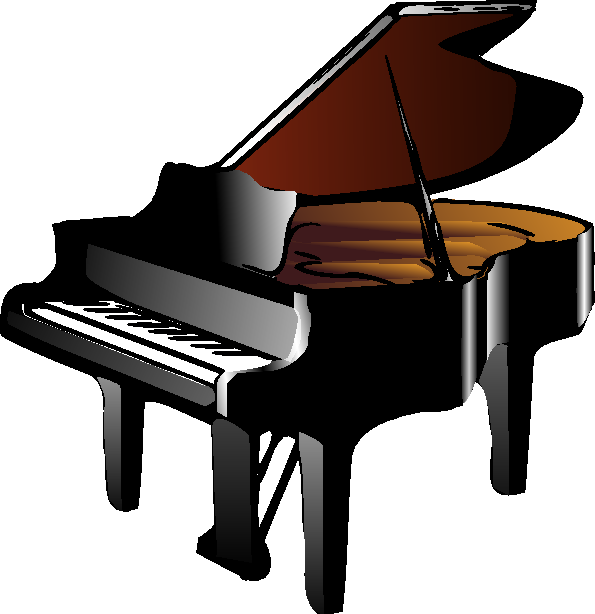
\includegraphics[scale=0.75]{piano}\\
\vspace{10em}
\href{http://www.pianopractice.org/}{Fundamentals of Piano Practice}\\
\href{http://www.pianopractice.org/}{http://www.pianopractice.org/}\\
\end{center}
\end{titlepage}

\begin{center}
Mojej žene\\
\vspace*{1em}
{\large Merry}\\
\vspace*{1em}
a našim dcéram\\
\vspace*{1em}
{\large Eileen a Sue-Lynn}\\	
\vspace*{6em}
\end{center}
\textit{Materiál prvej kapitoly pochádza z mojich poznámok, ako nebohá M\textsuperscript{lle} Yvonne Combe učila naše dcéry. M\textsuperscript{lle} Combe bola Debussyho žiačka a pomáhala prepisovať jeho nové kompozície ako ich hral na klavíri. Hrala ten neuveriteľný Druhý klavírny koncert od Saint-Saëns so skladateľom, ktorý dirigoval. Každé publikum ktoré sa zúčastnilo vystúpení jej študentov, obzvlášť keď hrali od Debussyho alebo Saint-Saëns, bolo fascinované. Bolo potrebné napísať túto knihu: bez tejto knihy by s jej odchodom tento svet prišiel o neoceniteľné umenie.}
\begin{center}
\vspace*{6em}
Kapitola Prvá: TECHNIKA HRY NA KLAVÍRI\\
\vspace*{1em}
Kapitola Druhá: LADENIE VÁŠHO KLAVÍRA\\
\vspace*{1em}
Použitá literatúra\\
\vspace*{10em}
6. marec 2009\\
Copyright \copyright 2009, kopírovanie povolené ak je uvedené autorovo meno,\\
Chuan C. Chang, a je zahrnuté toto vyhlásenie o autorstve.\\
ISBN: 1-4196-7859-0\\
ISBN-13: 978-419678592\\
Library of Congress Control Number: 2007907498\\
Objednajte si knihu na www.booksurge.com alebo Amazon.com\\
\vspace*{1em}
Celú knihu možno zadarmo stiahnuť zo stránky:\\

\href{http://www.pianopractice.org/}{http://www.pianopractice.org/}\\
Translation \copyright \the\year\ Ladislav Rado\\
\href{http://www.rsw.sk/piano/zaklady-cvicenia-na-klaviri/}{http://www.rsw.sk/piano/zaklady-cvicenia-na-klaviri/}
\end{center}

\cleardoublepage
\pagestyle{fancy}
\fancyhf{}
\fancyfoot[LE,RO]{\thepage}
\renewcommand{\headrulewidth}{0pt}
\renewcommand{\footrulewidth}{0pt}

\pagenumbering{roman} \setcounter{page}{1} 
\tableofcontents
\clearpage{\pagestyle{empty}\cleardoublepage}
\pagenumbering{arabic} \setcounter{page}{1}

\textbf{Prosba:} Tých, ktorí považujú túto knihu za užitočnú, prosím o to, aby dali vedieť o mojej webovej stránke aspoň dvom ďalším ľuďom a začali tak reťazovú reakciu, že viacero ľudí bude informovaných o tejto stránke. 
\medskip

\textbf{Hľadám dobrovoľníkov na preloženie tejto knihy} do akéhokoľvek jazyka. Pozri “Poznámky pre prekladateľov” na str. \pageref{subsec:poznamky-pre-prekladatelov}. Prosím pošlite mi mail na \href{mailto:cc88m@aol.com}{cc88m@aol.com} pre diskusiu ohľadom tejto veci. Táto kniha je v súčasnosti preložená do \href{http://bbs.popiano.org/viewthread.php?tid=192544&amp;extra=page\%3D1}{zjednodušenej čínštiny}, \href{http://www.pianogarden.tw/}{tradičnej čínštiny}, \href{http://www.sinerj.org/~loyer/fopp/}{francúzštiny}, \href{http://www.hansvanbreugel.nl/SnellerPianoStuderen/}{holandštiny}, \href{http://www.pianopractice.org/japanese.pdf}{japončiny}, \href{http://ko.wikisource.org/wiki/Fundamentals_of_piano_practice}{kórejčiny}, \href{http://www.makrai.net/balazs/fopp/contents.php}{maďarčiny}, \href{http://foppde.uteedgar-lins.de/index.html}{nemčiny}, \href{http://pianoart.eu.interiowo.pl/}{poľštiny}, \href{http://www.pianopractice.org/spanish.pdf}{španielčiny} a
\href{http://www.studiarepianoforte.it/}{taliančiny}.
\medskip

\textbf{Učitelia} môžu použiť túto knihu ako učebnicu pre vyučovanie metód cvičenia. Môže ušetriť mnoho času, umožňujúc im sústrediť sa na vyučovanie hudby. Predslov poskytuje dobrý prehľad o knihe a zhodnotenia v časti Použitej literatúry obsahujú detailné zhodnotenia najrelevantnejších kníh.
\medskip
           
\textbf{Študenti:} Ak nemáte učiteľa, vyberte si ľubovoľnú skladbu (ktorá je v rámci vašej technickej úrovne) a začnite cvičiť použitím metód opísaných tu; metódy sú usporiadané zhruba v takom poradí, ako ich budete potrebovať pri učení, keď sa začnete učiť novú skladbu. V každom prípade (s učiteľom alebo bez učiteľa), si prečítajte celú knihu rýchlo na prvý krát. Preskočte pasáže, o ktorých si myslíte, že nie sú dôležité alebo idú príliš do detailov; nesnažte sa porozumieť každému konceptu alebo si zapamätať čokoľvek – čítajte ako keby to bol román science fiction (ale nič z tohto nie je fikcia) – chcite sa len zoznámiť sa z knihou a získať predstavu, kde sú určité témy diskutované. Nakoniec si prečítajte časť Ohlasy podľa toho ako vás zaujmú.

Potom znovu začnite odtiaľ, kde si myslíte čo potrebujete; väčšina ľudí bude potrebovať prečítať celú kapitolu 1 časti I a II. Potom môžete preskakovať na konkrétne témy, ktoré sa vzťahujú na skladbu, ktorú sa učíte. Ak nemáte jasnú predstavu o tom, ktoré skladby sa učiť, táto kniha uvádza mnoho príkladov, od materiálu pre začiatočníkov (kapitola 1, III.18) po strednú úroveň, preto sa pri prvom čítaní pozrite, kde tieto príklady/návrhy sú.

\section*{Ohlasy}
\addcontentsline{toc}{section}{Ohlasy}
(Prijaté pred júlom 2004)\hfill
\vspace*{2em}
\newline
Tieto ohlasy ilustrujú nádeje, pokusy, trápenie, a triumf  klaviristov a učiteľov klavíra. Povzbudil ma počet učiteľov, ktorí poskytli ohlasy a ich indikácie toho, že majú väčší úspech so svojimi študentmi pomocou týchto typov metód. Zdá sa nevyhnutné, že učitelia, ktorí robia výskum a zlepšujú svoje vyučovacie metódy sú úspešnejší. Početní klaviristi uviedli, že boli učení predchádzajúcimi učiteľmi celkom zle. Mnohí, ktorí mali radi svojich učiteľov, poznamenali, že títo učitelia používajú metódy podobné tým, ktoré sú v tejto knihe. Je tam takmer jednotná zhoda v tom, čo je správne a čo je zlé, a preto, keď budete postupovať vedeckým prístupom, nedostanete sa do situácie, v ktorej sa ľudia nemôžu zhodnúť na tom, čo je správne. Bol som ohromený tým, ako rýchlo sa niektorí ľudia naučili tieto metódy.

Úryvky boli upravované minimálne, ale nepodstatné detaily boli odstránené tak, aby čitatelia nestrácali čas. Chcel by som poďakovať všetkým, ktorí napísali, pomohli mi tým zlepšiť knihu. Nemôžem sa dostať cez fakt, že čitatelia písali knihu spolu so mnou. (t.j. mohol som vložiť ich pripomienky do mojej knihy, a tie sa sem perfektne hodia!). V nasledujúcom texte som nevybral len  lichotivé poznámky, zvolil som materiál, ktorý sa javil významný (vzdelávací), či už bol kladný alebo kritický. Príspevky v [...] sú moje pripomienky:

1. [Od kresťanského kňaza]
Táto kniha je Biblia hry na klavír. Urobil som taký obrovský pokrok odvtedy, čo som si ju kúpil [1. vydanie knihy]. Aj naďalej ju odporúčam ostatným.
\medskip

2. [V januári roku 2003, som dostal tento email (s povolením)]
Moje meno je Marc, a mám 17 rokov. Začal som hrať na klavír asi pred mesiacom a čítal som vašu knihu, Základy hry na klavír. ... Ešte nemám učiteľa, ale nejakého hľadám. ... [Nasleduje rad predčasných otázok pre mladého človeka s tak málo skúsenosťami. Odpovedal som mu na otázky tak dobre, ako som mohol a potom v máji 2004 som dostal tento ohromujúci email]
\smallskip

Neočakávam, že si ma budete pamätať, ale poslal som vám e-mail o niečo viac ako pred rokom... Chcel by som, aby ste vedeli, ako sa vyvíjala moja hra na klavíri použitím vašej metódy. Začal som hrať na klavír na Vianoce roku 2002, od začiatku pomocou vašej metódy. V strede marca 2003, som na mojej strednej škole sa zúčastnil koncertnej klavírnej súťaži pre zábavu a skúsenosti - nie v nádeji na víťazstvo 500 dolárového štipendia. Nečakane som vyhral prvé miesto, pritom som súťažil s klaviristami ktorí hrali aj desať rokov. Porotcov šokovalo, keď som im povedal, že som hral len 3 mesiace. Pred pár dňami som vyhral rovnako aj tohtoročnú súťaž,. Inými slovami, pokrok prišiel veľmi rýchlo. Takýto pokrok je jednou najväčšou motiváciou (okrem všeobecnej lásky k hudbe), takže teraz sa vidím sám seba hrať - a zlepšovať sa – na klavíri po celý zvyšok môjho života. A aj keď musím uznať rovnako zásluhy mojich učiteľov, vaša metóda je základ, na ktorom stavali, a verím, že to je hlavným dôvodom môjho pokroku. Napriek tomu som stále považujem za začiatočníka... Môj web má všetky nahrávky, ktoré som urobil, do dnešného času (18). ... Nedávno som bol znovu nahrával Chopinove prelúdium “Dažďová kvapka”, Scarlattiho K.466, a Bachovu invencia v F dur. ... Mojou ďalšou nahrávkou bude Bachova Sinfonia v E moll, a mám v pláne ju urobiť do konca budúceho týždňa. Vaša kniha je omnoho viac než ktorýkoľvek milovník hudby a klavíra mohol očakávať, a nemôžem vám poďakovať za pomoc akú ste mi dali pre mnoho ďalších ašpirujúcich klaviristov. ... [Choďte na webové stránky a vypočujte si tie úžasné nahrávky! Môžete ho dokonca nájsť na internetovej stránke Music Download (hľadajte Marc McCarthy).] 
\medskip

3. [Od rešpektovaného, skúseného učiteľa klavíra.]
Len som rýchlo prezrel vašu časť [o paralelných cvičeniach] a myslel, že by som sa mohol podeliť o moju prvú reakciu. Ako odporca, som loboval hlasne a silno pre trestuhodnosť Hannonových a podobných cvičení a bol najprv zdesený pomyslením na tom, že ste sa pripojili k utláčaným masám pseudo-voodoo-esquí praktikantov, beznádejne, bezmocne, opakujúc, opakujúc, ... Mimochodom, aby som sa dostal k veci, vo vašom prístupe vidím hodnotu ak, ak, ak študent nasleduje tieto vaše ÚPLNÉ pokyny a používa kľúčové kombinácie ako diagnostický nástroj – NEOPAKOVAŤ každú kombináciu ako dennú rutinu. Ako diagnostický nástroj a následné odstránenie chýb, sa vám to podarilo skvele! Vaše cvičenia boli v niečom podobné, a tak som dnes zašiel do štúdia a našiel Technische Studien od Louis Plaidy, Edition Peters, prvé vydanie rok okolo 1850. Hoci Plaidyho filozofia týkajúce sa používania jeho cvičení je veľmi odlišná od vašej, skutočné noty tlačené na stránke sledovať takmer do písmena (no, mal by som povedať do noty), s tým čo ste popísali v kapitole o cvičeniach. Plaidyho cvičenia boli v Európe veľmi rešpektované ku koncu 19. storočia a boli použité v tej dobe na konzervatóriu v Lipsku. Plaidy bol celkom vyhľadávaný inštruktor, niekoľkí jeho študenti boli prijatí do vnútorného kruhu Liszta a/alebo mali nejaký úspech na koncertnom pódiu. Si v spoločnosti významných osobností! 
\medskip

4. Som zvedavý, či viete o práci od Guya Maiera. Je jeho prístup “impulzového” cvičenia vzorov pre 5 prstov podobný tým “paralelným sadám”, ktoré zmieňujeme? Maier používa princíp opakovania jednej noty každým prstom pričom ako ostatné sú v pokoji na povrchu ako jedno z 5 prstových cvičení. Thinking Fingers bola jedna z kníh cvičení, ktorú Maier napísal Herbertom Bradshawom v skorých 1940 rokoch. Jedno z jeho prvých 5 prstových cvičení, ktoré odzrkadľuje to, čo ste povedali o opakovaní “štvoríc” na jednej note jedným prstom je takéto:\\
a. Jednotlivé prsty v opakovaných impulzoch nôt 1, 2, 3, 4, 8 a 16.\\
b. Cvičenie každého prsta zvlášť, ostatné klávesy ľahko stlačiť  alebo držať prsty v pokoji na vrchnej pozícii klávesu.\\
c. Použitím CDEFG v pravej ruke, položte 5 prstov na tieto noty jednu oktávu nad stredným C, palec pravej ruky na C.\\
d. Podobne ľavú ruku, jednu oktávu pod stredným C, s piatym prstom na C.\\
e. Cvičte ruky zvlášť, počnúc palcom pravej ruky hrať jeden impulz C, potom uvoľniť, potom dva impulzy, atď, až 16. To isté opakujte s každým prstom, potom ľavou rukou.
[Pozri moje cvičenie v časti III.7b, je to úžasné, ako sme sa nezávisle dospeli k skupinám “štvoríc” (štyri opakovania), až 4 štvorice (16 opakovaní) pre toto cvičenie, ktorý je takmer totožný s mojím cvičením č.1.]\\
f. Začiatočníci by mali robiť impulzy pomaly, postupne sa prepracovať až do plnej rýchlosti (a tu myslím, že vaše “štvorice”, vstupujú do hry - toľko opakovaní za sekundu, je cieľ).
Maier zmienil 16 ako jeho limit. Veľa vzorov pre použitie tohto prístupu na 5 prstové impulzné cvičenia dáva, v Knihe 1 a Knihe 2 Thinking Fingers  publikovanej Belwin Mills Inc, NY, NY v roku 1948. Myslím, že Maier sa snažil pomôcť študentom získať obratnosť, ktorú potrebovali bez nekonečného opakovania cvičení od Hanon, Pischna, a iných. 
\medskip

5. Prosím, pošlite mi vašu knihu - Bol som učiteľom klavíra viac ako 50 rokov, a stále som dychtivý sa učiť.
\medskip

6. [Tento ohlas vám otvára oči: učí nás o jednej z najčastejšie zle vyhodnoteného problému, ktoré sa zastaví nás hrať rýchlo.]
V mladom veku, som začal, a potom ukončil hru na klavír. Potom sa ako teenager, som šiel na [slávne] konzervatórium a roky sa snažil získať techniku, ale neuspel som a skončil s inžinierskou kariérou. O niekoľko rokov neskôr, som sa vrátil ku klavíru (Clavinova) a snažím sa robiť to, čo som nedokázal urobiť rokmi. Jedným z dôvodov, prečo som prestal cvičiť, bolo že moja žena a syn boli podráždení, keď ma počuli opakovať pasáže znovu a znovu; Clavinova mi umožňuje cvičiť beztrestne v akúkoľvek hodinu. Čítal som vaše webové stránky a bol fascinovaný. Kiež by som mohol premýšľať o niektorých z vašich nápadov pred rokmi. Mám otázku a ja nedokážem dostať odpoveď, ktorá dáva zmysel, ale je to základná otázka. Učil som sa, že keď ste hrať na klavír, podporujete váhu ruky na každý prst, ktorý hrá. Gravitácia. Nikdy netlačíte dole, musíte byť zrelaxovaný. Tak som sa pýtal svojich učiteľov, ako sa hrá pianissimo. Odpoveď znela, že hráte bližšie ku klávesom. To pre mňa nefungovalo. [Dlhá diskusia o rôznych metódach snaženia sa hrať pianissimo s váhou ramena a prečo nefungujú. Zdá sa, že môže hrať pianissimo iba vedome zdvihnutím ruky preč z klávesov. A tiež, pretože všetko, má tendenciu vychádzať forte, rýchlosť je problém.] Mohli by ste láskavo odpovedať na túto otázku pre mňa? Čo sa dá robiť s váhou ramena, keď sa hrá pianissimo? Čítal som veľa kníh o hraní na klavír, a hovoril s mnohými uznávanými klaviristami. Jedna vec je vedieť, ako hrať čokoľvek a celkom iná, učiť niekto, ako hrať. [Nemohol som povedal to lepšie!] Vaše spisy sú pozoruhodné a v mnohých ohľadoch revolučné, vedel som inštinktívne, že keby mi niekto mohol pomôcť,  mohli by ste to byť vy. 
[Po takomto komplimente, som musel niečo urobiť, tak som si starostlivo prečítal jeho objasnenie ťažkostí a dospel k záveru, že musí, po toľkých rokoch snaženia, nevedomky tlačiť do klavíra, skoro ako by bol zhypnotizovaný. Povedal som mu aby našiel spôsob, ako zistiť, či bol skutočne tlačí nadol – nie je to ľahká úloha. Potom prišla táto odpoveď.]
Ďakujem vám za vašu reakciu. Pravda je najlepšie zisťované prostredníctvom extrémov. Váš návrh mi vnukol myšlienku, že by som mal VŽDY hrať tak ako by som hral MOJE pianissimo – zdvihnutím rúk od kláves. A prešiel som môjmu Hanonovi, a ÁNO! Dokážem hrať oveľa rýchlejšie! Ďalej som rýchlo prešiel k Bachovmu Prelúdiu II, ktoré som nikdy nemohol hrať v tempe (144) a vždy som mal problémy aby prsty dopadali spolu pri rýchlom hraní, a pri rýchlostiach nad 120 prsty dopadali ako jedna nota spolu. Žiadna nešikovnosť, žiadne napätie. Nielen, že môžem hrať na piano, alebo forte tak rýchlo, ako ja chcem. To je tak neuveriteľne ĽAHKÉ! Len teraz som to objavil! Nemôžem tomu uveriť. [Dlhá diskusia o tom, ako, v priebehu rokov, došiel k tomu aby vyrovnal váhu rúk tlačením nadol, spôsobené hlavne strachom z nepochopenia učiteľa, ktorý bol prísny a dbal na váhu rúk. To je vlastne niečo, k čomu som mal veľkú nedôveru, o metóde váhy rúk: že tak veľký dôraz váhu ruky a prehnaná prísna disciplína môže spôsobiť nejaký druh neurózy alebo nedorozumenia – možno aj nejaký druh hypnózy.] Obrovský múr sa jednoducho rozpadol a teraz po toľkých rokoch myslenia a hodín cvičenia (cvičil som až 10 hodín denne na konzervatóriu a len som si zapamätal hudbu, bez zlepšenia mojej techniky) a teraz vidím za hranice. Zistil som, že mám možnosť hrať rýchlejšie, než som kedy sníval som mohol (len som skúsil stupnicu C dur, a bol som šokovaný, že som to bol ja kto hral) s plným rozsahom zvuku, ktorý chcem bez napätia. [Dlhý popis všetkých nových vecí, ktoré teraz robí a ich porovnanie s jeho predchádzajúcimi rokmi námahy a kritiky od ostatných.] Musím vám za to poďakovať. Vaša bola jediná kniha, ktorú som čítal a ponúkla mi dostatok variácií  od hlavného prúdu, aby ma konečne zbavila moju myseľ z veľkého nepochopenia. Tlačilo som dole a nenechal som to ísť. Moje ruky jednoducho nevážia tonu, ale sú voľné. Pretože som mal strach a môj učiteľ bol posadnutý s váhou mojich rúk, podvedome som ich tlačil nadol. Nikdy som sa pre ňu neodvážil hrať \noteDynamics{ppp}. Vedel som ako, ale bol som si istý, že bola zlá technika. [Obávam sa, že sa to stane často mládeži; nechápu učiteľa, ale boja sa opýtať, až skončia s prijatím zlej veci.] To, čo mi mala povedať bolo NIKDY NETLAČ DOLU; namiesto toho som sa zafixoval na váhu rúk ako kľúč ku všetkému. [Mladík musí tlačiť dole, aby dal nejakú “váhu” na ruky! Ako budete vysvetľovať, že to je zlé, dieťaťu, ktoré neštudovalo fyziku?] Ona tiež nikdy nedovolila, aby som sa hral rýchlo. [To je ďalší komentár, ktorý som počul od študentov učiteľov prísnych na hmotnosť rúk - rýchlosť je no-no, pokým nie sú dosiahnuté určité míľniky, aj keď musíme cvičiť opatrnosť pri cvičení pre rýchlosť, spomalenie nie je najrýchlejší spôsob, ako zrýchliť.] Vzhľadom na to, že som bol napätý, povedala že nikdy nebudem môcť hrať rýchlo ak som napätý. Vo svojej knihe hovoríte, že by sme mali hrať rýchlo aby sme objavili techniku. Ja som to  nikdy nemal dovolené! Vaša kniha a vaše e-maily uvoľnili  reťaze v mojej mysli, ktoré ma držali v zajatí všetky tie roky. Veľakrát vám ďakujem. Nedokážem opísať, ako som vďačný vám a vášmu pochopeniu. [Aj keď moje poznámky sa zdajú byť namierené proti škole váhy rúk, nie je to tak –  podobné ťažkosti sa vzťahujú na všetky učenia založené na nedostatočnej znalosti rúk prísnych učiteľov. Bohužiaľ, veľké množstvo klavírnych učiteľov historicky prijala nepružné metódy výučby z dôvodu nedostatočných teoretických vedomosti a racionálne vysvetlenia. Pre systematické zušľachťovanie rýchlosti, pozri body II.13 a najmä III.7.i]
\medskip

7. Našiel som vašu knihu na internete a považujem to za veľké šťastie. Veľmi vám ďakujem za vyvinutie takého veľkého úsilia na opis techniky hry na klavír a cvičebné návyky, ktoré dávajú zmysel. Som učiteľom klavíra. Len som začal čítať knihu a už som uplatnil niektoré techniky cvičenia s mojimi študentmi. Im sa to páčilo a mne tiež. Cvičenie sa stáva oveľa zaujímavejším. Viete o knihe s názvom “Spoločník Amatérskeho Klaviristu” od James Ching, vydané Keith Prowse Music Publishing Co, 1956, Londýn. Táto kniha môže byť vypredaná, ale našla som ju z druhej ruky na adrese:
http://dogbert.abebooks.com/abe/BookSearch
Mohlo by vás to zaujímať, pretože “detail správneho držania tela, pohyb a podmienky, ako je uvedené v tejto knihe sú výsledkom rozsiahlych výskumov fyziológie-mechaniky klavírnej techniky vykonávané podľa autora v spolupráci s profesorom H. Hartridge, profesor fyziológie, a H. T. Jessop, lektor mechaniky a aplikovanej matematiky na University of London”.
\medskip

8. Som tak vďačný, že som našiel vaše webové stránky. Som dospelý hráč na klavír, ktorý keď bol mladý sa učil všetko zle. Stále sa snažím odnaučiť moje zlé techniky a návyky. Teraz chodím na hodiny k veľmi dobrému učiteľovi.
\medskip

9. Pred niekoľkými týždňami som si stiahol vašu knihu z internetu, skúšal som to. Som asi v polovici a ďaleko od úplného uplatňovania všetkého, ale som tak spokojný s výsledkami doteraz, že som si myslel, že by som mohol dať spontánne nejakú spätnú väzbu.
Najprv niečo z pozadia. Študoval som klavír až do pokročilej úrovne a začal hudobný titul, ktorý som skončil po tom čo som rok študoval matematiku. Po ukončení školy som bol nadšený amatér, ale v priebehu posledných 20 rokov moje hranie bolo menej časté, hlavne kvôli môjmu sklamaniu z nedostatočného pokroku, presvedčený o tom, že nikdy nebudem schopný nájsť hodiny na cvičenia potrebné na to, aby som hral lepšie. Hľadal som niekoľko rád pre nákup klavíra a prišiel som na vašu stránku. Po prečítaní niekoľkých kapitol som sa stiahnuť celú knihu a začal som skúšať. Nie je to prvýkrát, čo som sa snažil zlepšiť s knihou alebo radou od učiteľa, ale ja som obetný baránok. Tu sú moje skúsenosti po troch týždňoch. [Všimnite si, ako rýchlo sa ľudia môžu naučiť a okamžite využiť tieto metódy.]\\
Sústredil som sa na štúdium 4 skladieb, ktoré sú veľmi drahé pre mňa:\\
- Ravelovo prelúdium\\
- Chopinovo prelúdium č. 26 v As dur\\
- Poulencovo Novelette č. 1\\
- Ravelova Alborada del Grazioso z Miroirs\\
Ravelovo prelúdium je malá skladba bez žiadnych zjavných technických ťažkosti. To je skladba, že som vždy hral na prvý pohľad, ale nikdy naozaj dobre. Je v nej časť s prekrížením rúk v strede s niektorými nádhernými disonanciami, ktorá predstavuje určité ťažkosti, ale to je tak všetko. Uplatnil som cvičebné metódy v knihe na tento kúsok a zrazu ožil s oveľa väčšou nuansou, akú som jej kedy pripisoval. Skladba je niečo, o čom som si myslel, že je na zahodenie, ale bez riadnych metód cvičenia sa tak bude zdať vždy.
Poulenc Novelette je jeden z kúskov, ktoré som hral aspoň raz týždenne po dobu 20 rokov a som  naň veľmi hrdý. Nikdy som to naozaj nehral k mojej plnej spokojnosti, ale vždy som predpokladal, že to bolo vďaka nedostatku času cvičenia. Použitím vašich návrhov som začal analyzovať, čo bolo zle. Okrem niektoré zjavných chýb ktoré neboli odstránené, najprekvapujúcejším výsledkom bolo, že som nebol schopný udržať tempo s metronómom!! Podrobnejšia analýza odhalila príčinu – veľa skladieb napísaných Poulencom vyžaduje rýchly a čudné posuny polohy rúk, s melódiami, ktoré treba udržať medzi týmito posunmi. Zlozvyk, ktorý som sa naučil, bolo “chytiť” klávesy počas týchto posunov, a teda ničiť melodickú líniu a postupne to zrýchľovať. Pre mňa objavom, bolo to, že problém nemôže byť vyriešený cvičením s metronómom! Mohlo to byť vyriešené len analyzovaním tohto problému a vypracovaním stratégie ako si poradiť s týmito posunmi. Teraz som veľmi spokojný s tým, ako hrám a dokonca mi veľa času zostane, aby som sa zaoberal hudbou.
Alborada del Grazioso je prípad sám o sebe. To je diabolsky obtiažny kus, ktorý som sa snažil učiť v minulosti, ale nebol schopný priniesť väčšinu pasáží na správnu rýchlosť. Môj predpoklad bol vždy ten, že bolo nevyhnutného viac cvičenia a že som si naň nikdy nemohol nájsť čas. Opäť – použitím metód  z vašej knihy na učenie tohto, po troch týždňoch, ešte nie som na konci, ale už teraz môžem hrať väčšinu z toho v rýchlosti a tiež rozumne hudobne. Hádam, budem mať to všetko v mojich prstoch, potom sa môžem sústrediť na hudbu.
V neposlednom rade, prelúdium od Chopina. Naučil som sa to na skúšku, keď som mal 16 rokov ale odvtedy som to nehral. Po prvé, nikdy som to nehral v tempe ani na skúške, takže to bolo niečo, čo som potreboval opraviť. Avšak toto jednoducho nefungovalo - zistil som, že z dvoch dôvodov som nemohol zrýchliť. Po prvé som sa naučil predstierať legato s pedálom - ale akonáhle zrýchlite dostanete nesúrodý zvuk a keď som pokúsil používať pedál správne nemohol som dostať legato. Po druhé, prostredná časť obsahuje niektoré veľmi roztiahnuté rozložené akordy v ľavej ruke ktoré sa posúvajú na každú dobu. Hrané pomaly je to v poriadku, ale pri rýchlosti sa to stáva diabolsky ťažkým a dokonca aj bolestným hrať. V podstate som sa musel znovu naučiť túto skladbu - nové prstoklady, nové pozície rúk, rozdielne používanie pedálu atď. Teraz už môžem hrať na ktorejkoľvek rýchlosti bez napätia. Našiel som toto ako zaujímavý dôkaz toho, čo hovoríte v knihe - to je veľmi malá skladba ktorá sa zdá byť pomerne jednoduchá, ale v rýchlosti úplne mení charakter a bude znechucovať každého študenta používajúceho intuitívne metódy, pokiaľ nie sú požehnaný s rozpätím viac ako 1,5 oktávy.
Na záver by som vám rád poďakoval za písanie knihy a ešte viac za jej sprístupnenie na internete. V minulosti som minul obrovské množstvo peňazí na vysoko odporúčaných učiteľov a ani jeden z nich, aj keď nemám pochýb o tom, že sami chápu tieto techniky, ma nemohol naučiť ako cvičiť.
\medskip

10. Myslím, že vaša kniha stojí za čítanie môj hoci mnoho z “pravidiel” (napr. cvičenie každej ruky zvlášť, útok akordu...) som sa naučil od našich učiteľov. Podľa mojej logiky, ak som sa naučil čo i len jedno pravidlo z vašej knihy, ktoré funguje, je to hodné oveľa viac, než 15 dolárov, ktoré som zaplatil za 1. vydanie. Tiež sa mi páči časť o tom, ako sa pripraviť na vystúpenia. Súhlasím s tým, že cvičenie v plnej rýchlosti pred vystúpením je “no no”. Prebral som to s mojím učiteľom a vidíme niekoľko dôvodov, prečo [rozšírené diskusie o tom, prečo hranie v plnej rýchlosti pred vystúpením môže viesť k problémom, neuverejnených tu pretože, im nemôžem porozumieť]. Teda cvičenie rýchlo pred vystúpením nie je výherná situácia. Na záver by som rád videl viac o tom, ako zvýšiť rýchlosť a ako dať hrať rukami spolu efektívnejšie. Niektorá hudba (Bachove Invencie mi prichádzajú na myseľ), je jednoduchá hrať zvlášť ale ťažko spolu. Celkovo môžem povedať, že ma baví čítanie vašej knihy.
\medskip

11. Nabádam každého, aby skúsil cvičenie rúk samostatne, ako sa uvádza vo vašej knihe. Pri štúdiu s Robertom Palmierim na Kentskej štátnej univerzite, som to musel som robiť ako súčasť môjho cvičenia. To mi pomohlo dostať cez amatérsku úroveň a na oveľa lepšiu techniku a hudobnú hru.
\medskip

12. Na základe toho, čo som bol schopný vyčítať z vášho webu, som praktizoval jednu z vašich zásad – hrať každou rukou zvlášť na plné tempo - na niekoľkých náročných pasážach v dvoch úplne odlišných typov skladieb, ktoré som hral, jedeným bol kostolný hymnus, ďalším jazzové melódie. Čo je zaujímavé, zistil som že, že keď som sa včera dostal do kostola a prišiel čas sprevádzať zbor, ťažké časti, ktoré som sa naučil s rukami zvlášť boli medzi najviac spoľahlivo a isto zahrané z celého hymnu. Zdalo sa, že zakaždým, keď som prišiel na jedno z tých ťažkých miest, spustilo sa v mysli upozornenie pre môj mozog/nervový systém vykonať tieto časti s mimoriadnou  starostlivosťou a presnosťou. To isté platí aj pre ťažké miesto v jazzovej melódii, ktorá je teraz už  vôbec nie je problémom.
\medskip

13. Asi pred jeden a pol rokom som si objednal knihu Základy cvičenia na klavíri od vás. Len som vám chcel osobne poďakovať za váš príspevok. Pomohlo mi to veľa! Nikdy pred vašou knihou som  nevedel ako cvičiť, pretože som sa to nikde neučil. Chodil som na hodiny, ako vy, ale moji učitelia ma nikdy nenaučili ako cvičiť. Nie je to úžasné! Pochybujem že je to samozrejmosť. Najprínosnejšie rada pre mňa je váš návrh hrať na oveľa pomalšie posledné prehratie skladby, ktorú cvičíte. Musím sa priznať, že vytvorenie tohto zvyku bolo pre mňa najťažšie. Ale ja sa snažím. Zistil som, že pomalé cvičenie je veľká pomoc. Tiež cvičenie len jedného alebo dvoch taktov bolo cenné! Prial by som si, aby zapamätanie hudby prišlo jednoduchšie, ak máte nejaké nové nápady na zapamätanie, dajte mi prosím vedieť. [Odvtedy čo som dostal túto korešpondenciu som pridal značný materiál na zapamätanie.]
\medskip

14. Ďakujem Vám za odpoveď na moje otázky ohľadom cvičenia na klavír. Musím vám povedať, že je tu jedno obzvlášť chúlostivé prelúdium od Chopina – to v C moll. Keď som dostal vašu knihu, zvládol som toto prelúdium do jeho rýchlosti za jeden deň. Pripusťme, je to krátke, ale mnoho klaviristov s ním zápasí. Táto skúsenosť bola veľmi povzbudivá.
\medskip

15. Hral som na klavíri doteraz 8 rokov a kúpil vašu knihu asi pred rokom. Po prečítaní tejto knihy, moja 1 hodina denného cvičenia je oveľa produktívnejšia. Tiež sa učím nové skladby oveľa rýchlejšie. Ukazujete podstatu nasledovného:\\
Správne metódy cvičenia\\
Ako začať novú skladbu.\\
Pomalé cvičenie (kedy ho robiť a prečo).\\
Kedy hrať rýchlejšie, než je obvyklé.\\
Ako sa pripraviť na vystúpenie.\\
Nesúhlasím so všetkým, čo píšete, ale čítam vašu knihu každých pár mesiacov, aby som nestratil správny podhľad na to ako cvičiť. [To je všeobecný refrén: Moja kniha je taký hustý kompilát, že ju musíte prečítať niekoľkokrát.]
\medskip

16. Po jednom týždni, bol som veľmi potešený sám so sebou, a metódou, pretože som si myslel, že som si úspešne ZAPAMÄTAL{\noligatures !!!} celú stránku hrané každou rukou zvlášť. To bolo úplne neznámym úspechom, pokiaľ išlo o mňa. Ale problémy nastali, keď som sa snažil dať dohromady dve ruky, ktoré som potom sa snažil robiť, zatiaľ čo som sa učil zvyšok skladby. Tiež som zistil pri snažení sa naučiť zvyšok skladby, že som si zle 'zapamätal' prvú stránku, a skončil som písaním nôt pre seba. [To sa pravdepodobne stane častejšie, než by si väčšina z nás chcela priznať, - ak máte ťažkosti s dostaním sa rýchlosť rukami spolu, OVERTE SI NOTY! Príčinou môže byť chyba pri čítaní hudby. Chyby v rytme sú obzvlášť veľmi ťažké odhaliť.] Vaša kniha mi dala presne to, čo som hľadal – t.j. nejaký základ pre to ako sa učiť pri cvičení rýchlejšie a efektívnejšie. Žiaden učiteľ mi nebol nikdy schopný dať mi oporný bod ako sa učiť skladbu. Jediným návrhom ktorý som kedy mal, je, 'Pozrite sa na toto a uvidíte, čo s tým môžete urobiť', a pokiaľ ide o ako zlepšiť presnosť a/alebo rýchlosť, 'Neprestávajte cvičiť, cvičiť... ' ČO????? Teraz som dostal odpovede na tieto zásadné otázky. Vďaka.
\medskip

17. Čítal som vašu knihy na vašich stránkach a veľa som z nej získal. Inšpirovali ste ma k cvičeniu spôsobom, o ktorom som vždy vedel, že je to najlepší spôsob, ale nikdy som na to nemal trpezlivosť. Čo vám naznačujete o vyrovnaných akordoch pred tým než sa pokúsite hrať rýchle línie, či určite mi pomohlo veľa. Myslím, že moja neschopnosť hrať nad určitú rýchlosť je spôsobená základnou nerovnomernosťou v mojich prstoch, ktoré som nikdy neriešil. Vždycky by som len povedal: “Ja jednoducho nemôžem hrať dobre rýchlo”. Vypracoval som sa malú časť etudy s použitím prístupom útoku akordov a môžem skutočne hrať pomerne hladko a rovnomerne! Som zvedavý na vaše teórie o rozvoji absolútneho sluchu. Tábory sa zdajú veľmi rozdelené na túto tému: genetika verzus životné prostredie. [Odvtedy čo prišla táto korešpondencia, som pridal paralelné cvičenia pre cvičenie akordov, a napísal rozšírené časť o získaní absolútneho sluchu.]
\medskip

18. Len som chcel, aby ste vedeli, ako moc sa moja rodina hudobníkov tešila z vašej knihy o výuke hry na klavíri. Bezpochyby ste posunuli nejaké inovatívne, neortodoxné myšlienky vo svojej knihe, ktoré naozaj robia nejakú prácu a to aj napriek faktu, že pre mnohých učiteľov znejú extrémne. [Súhlasím!] Metóda cvičenia rúk zvlášť zdá sa pracuje celkom dobre, rovnako ako spôsob nehranie  všetko veeeeeeľmi pomaly! Tiež sa ukazuje pozitívny vplyv keď sa kladie menší dôraz na metronóm. Iste, vaše metódy pomohli urýchliť celý proces učenia sa nových skladieb, a teraz si už neviem predstaviť, ako sa nám to podarilo pred bez znalosti týchto “hudobných právd” od vás. Ešte raz vám ďakujem za napísanie nádherného KLENOTU akým je táto kniha!
\medskip

19. Čítal som časti knihy z internetu a myslím si, že od každého učiteľa klavíra by sa malo požadovať, aby si prečítal túto knihu. Som jeden z nešťastník, ktorý strávil 7 rokov cvičením stupníc/Hanona bez akýchkoľvek náznakov relaxácie alebo efektívnych metód cvičenia. Začal som si získavať dobré rady pre cvičenie z internetových diskusných skupín a rôznych kníh, ale vaša kniha je zďaleka najkomplexnejšia a najpresvedčivejší zdroj, ktorý som doteraz našiel.
\medskip

20. Som hráč na klavír na stredne pokročilej úrovni. Pred mesiacom som stiahol časti vašej knihy a musím povedať jedným slovom, že to je obdivuhodné! Ako vedec oceňujem štruktúrovanú podobu prezentovania a prozaické vysvetlenie. Zmenilo to môj pohľad na cvičenie hry na klavír. Zvlášť časť o zapamätávaní mi pomohla značne zníženiu úsilie na zapamätanie. Môj súkromný učiteľ (koncertný sólista) používa kúsky z vašej metódy. Avšak tento učiteľ je zástanca Czerného a nikdy nepočul o technike hrania palec cez. Mali by ste venovať viac pozornosti technike palec cez, a to najmä, ako hladko spojiť paralelné sady. Dal som kópiu knihy môjmu učiteľovi a odporúčam ju každému.
[O rok neskôr]
Už som vám písal kedysi pred viac ako rokom o vašej fantastickej knihe na internete. Metódy naozaj fungujú. Použitím vašich metód som bol schopný sa naučiť a zvládnuť niektoré skladby oveľa rýchlejšie. Vaše metódy naozaj fungujú pre skladby, ktoré sú notoricky ťažké na zapamätanie, ako napríklad niektoré sonáty od Mozarta, a kúsky, ktoré môj učiteľ klavíra povedal, že sú ťažké si zapamätať, ako sú Bachove Invencie alebo niektoré prelúdiá od Chopina. Ako hračku teraz riešim Fantaisie Impromptu a tento zdanlivo nemožná skladba sa zdá byť v mojom dosahu! Tiež sa mi páči váš príspevok o podvedomí. Zaujímalo by ma, či viete o knihe J.D. Sarno: The Mindbody Prescription. Táto kniha pojednáva o podvedomí presne ako vy. Pri práci na svojej dizertačnej práci, som vyriešil veľa zdanlivo neriešiteľných teoretické hádaniek, rovnako ako vy. Nakŕmil som nimi svoj mozog a o niekoľko dní neskôr riešením proste vyskočili. Takže to, čo píšete, je úplná pravda!
\medskip

21. Vaše návrhy na to, ako si zapamätať hudby tým, že vytvoria asociácie (napríklad príbeh), znelo pre mňa hlúpo. Ale keď som cvičil, nemohol som sa neprestať pýtať, čo by som si mohol spájať s istou hudobnou frázou, ktorá mala problematický F akord. “Daj si F pre nedostatok” vyskočilo do mojej mysle. Myslel som, že nebolo moc povzbudivé myslenie! Ale teraz zakaždým, keď som prišiel, že veta Spomínam si, F. Mám to. Fíííha! Vďaka. Vaša kniha je veľmi užitočná. Odráža návrhy môjho učiteľ, ale s viacerými detailmi. Keď nemôžem hrať na klavír, nič nie je väčšia zábava, ako čítanie o hraní na klavír... ... ..f. V posledných týždňoch pred mojím posledným vystúpením, môj učiteľ navrhol hranie cez moje chyby počas cvičenia. Potom sa vrátim a pracujem na problémových taktoch, rovnako ako navrhujete, aj keď toto bol jediný čas, kedy som k tomuto pristúpil. Povedala, že väčšina ľudí ani nevie chyba nastala pokiaľ nedošlo k prerušeniu hudby. Jej pointa je neprerušiť hudbu a odstránenie zdroja pri návrate k určitému taktu. Zistil som, že sa veľa opravujem (zadrhávam), sústredím sa na to aby som to nerobil. Táto rada nie je intuitívne, veď viete. Človek opravuje chyby prirodzene, keď k nim dochádza. Ale vidím, že neustálym robením tohto sa v skutočnosti vytvárajú chyby.
\medskip

22. Narazil som na vašu on-line knihu o cvičení hry na klavír, keď som hľadal články o absolútnom sluchu. Keď som ju čítal, bol som ohromený tým, že bol použitý vedecký prístup. Zvlášť pojem “rýchlostného múru” a ako ho prekonať mi veľmi pomohol. Našiel som vašu knihu v správnom čase. Veľa problémov s ktorými sa stretávam pri hre na klavíri diskutujete vo vašej knihe. Mnohí učitelia klavíra zdá sa nemajú jasný vedecký koncept o tom, ako zvládnuť špecifické problémy pre hráčov na  strednej úrovni. Takže pracovať podľa knihy, po častiach s dobrým úspechom. Existuje niekoľko vecí, ktoré mi chýbajú vo vašej knihe. V niektorých kapitolách, by boli veľmi užitočné obrázky, ako je správna poloha rúk, palcom cez, a cvičenia paralelných množín. Niečo ako chronologické tabuľky pre cvičebnú rutinu by mohli byť užitočné. “Nácvik bez rozohratia”, by napríklad mohol byť na pozícii číslo jedna. Vždy sa zmienite o dôležitosti toho KEDY a ČO. Mohli by ste usporiadať cvičenia, ktoré vysvetľujete tak, aby ste ich urobili čo najefektívnejšie? Mimochodom, chcem vyjadriť svoje hlboké uznanie pre váš projekt!
\medskip

23. Celú túto zimu som pokračoval v osobnom učení hry na klavíri a musím povedať, že každé slovo v tejto knihe je pravda. Študoval som klavír niekoľko rokov dosiahol len priemerný pokrok. Pretože milujem klavír a romantickú hudbu, ktorá ma občas poblázni a frustruje. Po uplatnení vašich metód asi pred 1 rokom, som urobil obrovský pokrok. Teraz pracujem na niekoľkých skladbách naraz,  skladby o ktorých som si nikdy nemyslel že môžem hrať. Je to obdivuhodné. Dnes mám malý repertoár, ktorý môžem hrať s veľkým uspokojením.
\medskip

24. Objednal som si a dostal vaše prvé vydanie knihy a čítal som časti z druhého vydania. Zistil som, že vaše informácie sú veľmi cenné. Posielam vám tento e-mail, pretože som dúfam že mi dáte nejaké rady pred mojim blížiacim sa koncertom. Som veľmi nervózny, ale po prečítaní vašich častí o vystúpeniach chápem ich dôležitosť. Kiež by som mal vaše poznámky o zapamätávaní, keď som začal učiť, pretože mi to trvalo veľmi dlho, než som si skladbu konečne zapamätal (nesprávnym spôsobom). Nie som si istý, ako hrať skladbu na vystúpení. Pri niekoľkých príležitostiach, kedy som hral skladbu pred ostatnými by som sa zasekol na určitých úsekoch, pretože som zabudol, kde som bol kvôli nervom. Toto je moje prvé vystúpenie, takže neviem čo očakávať. Akékoľvek tipy a rady o praxi rutiny by sa veľmi páči.
[Po niekoľkých výmenách o tom, čo hral, atď., som mu dal scenár typických cvičebných rutín pre prípravu na vystúpenie a čo očakávať v priebehu vystúpenia. Po vystúpení, som dostal nasledujúci e-mail.]
Len som chcel, aby ste vedeli, že moje vystúpenie dopadlo veľmi dobre keď zvažujem, že bolo moje prvé. Rada ktorú ste mi dali bola veľmi užitočná. Bol som nervózny pri začínaní skladby, ale potom som sa veľmi sústredil (presne ako ste povedali, že sa stane). Bol som dokonca schopný sústrediť na hudbu než len prechádzať cez pohyby. Publikum bolo očarené mojou schopnosť hrania spamäti (rovnako ako ste povedali, že by mohlo byť). Mali si pravdu v tom, že pozitívna skúsenosť, ako je táto mi mohla pomôcť so sebadôverou. Cítim sa skvele po tejto skúsenosti! Môj učiteľ [je zo slávneho konzervatória] učí cvičenia od Hanona a iný technický materiál. To je dôvod, prečo vaša kniha bola a je pre mňa zlatou baňou. Chcem byť schopný hrať skladby, ktoré ma bavia, bez toho aby museli stráviť 20 rokov, aby som sa ich naučil. Ale tiež mám pocit, že potrebujem učiteľa.
\medskip

25. [Napokon, stovky oznámení typu:]
Musím povedať, že vaša kniha je vynikajúca{\noligatures ........} \\
Odvtedy čo som čítal C. C. Chang: Základy hry na klavír, som skúšal jeho návrhy; vďaka tým, ktorí mi ju odporučili a pánovi Changovi že si našiel čas ju napísať a dať ju k dispozícii. \\
Atď., atď.
\medskip

Od júla 2004 (kedy som uzavrel túto časť Ohlasy), som aj naďalej dostával e-maily podobné, najmä od študentov hudobných konzervatórií. Najviac potešujúce je zvyšujúci sa počet učiteľov, ktorí hovoria, že sú úspešne používajú tieto metódy pri výučbe, a že ich študenti sú šťastnejší a robia rýchlejší pokrok. 

\newpage
\section*{Skratky a často používané frázy}
\addcontentsline{toc}{section}{Skratky a často používané frázy}
Oddiely (...) sú v prvej kapitole, pokiaľ nie je uvedené inak
\vspace*{2em}
\newline
\noindent\textbf{SKRATKY}\\
AS = Absolútny sluch (III.12)\\
RL = Rovnomerné ladenie (Kap. 2, časť 2c \& 6c)\\
PVP = Pozícia vystretých prstov (III.4b)\\
FI = Fantaisie Impromptu od Chopina (II.25, III.2\&5)\\
DRH = Degradácia rýchleho hrania (II.25, ku koncu kapitoly)\\
RZ = Ruky zvlášť (II.7)\\
RS = Ruky spolu (II.25)\\
K-II = Kirnbergerov II Temperament (Kap. 2, časť 2c \& 6b)\\
ĽR = Ľavá ruka\\
HM = Hranie v mysli (pozri Index)\\
RJ = Rast jadra (III.15)\\
ZPC = Zlepšenie po cvičení (II.15)\\
PS = Paralelné sady (pozri nižšie)\\
PR = Pravá ruka\\
RSt = Rýchlostná stena (III.7i)\\
PC = Palec Cez (III.5)\\
PP = Palec Pod (III.5)\\
TL = Temperované ladenie (Kap. 2, časť 2c)
\vspace*{3em}\\
\noindent\textbf{Často používané frázy}\\
Metóda vozíka (III.5, v časti o rozložených akordoch)\\
Útok akordu (II.9)\\
Spojenie (II.8)\\
Strnulosť otočenia (III.4b)\\
Intuitívna metóda (II.1)\\
Hra v mysli (II.12, III.6j)\\
Paralelné sady (II.11, III.7b, pozri Index)\\
Pozícia Pyramídy = pozícia “ploché prsty” (III.4b)\\
Tiché ruky (III.6l)\\
Cvičenie po úsekoch (II.6)\\
Rýchlostná stena (III.7i)\\
Pozícia Pavúka = pozícia “ploché prsty” (III.4b)
\newpage

\section*{Predslov}
\addcontentsline{toc}{section}{Predslov}
\emph{Toto je najlepšia kniha, aká kedy bola napísaná o tom, ako cvičiť na klavíri!} Objavom tejto knihy je, že existujú vysoko efektívne metódy cvičenia, ktoré môžu urýchliť vašu rýchlosť učenia až 1000 krát, ak ste sa doteraz nenaučili najúčinnejšie metódy cvičenia (pozri IV.5). Prekvapivé je, že aj keď tieto metódy boli známe od počiatkov hry na klavíri, zriedka boli vyučované, pretože len málo učiteľov o nich vedelo a títo znalí učitelia sa nikdy neobťažovali, aby šírili tieto vedomostí.
\medskip

\emph{V roku 1960 som zistil, že neexistovala žiadna dobrá kniha o tom, ako cvičiť hru na klavíri.} Najlepšie, čo som mohol nájsť bola kniha od Whitesideovej, ktorá bola úplným sklamaním, pozri moju recenziu tejto knihy v odkazoch. Ako postgraduálny študent na Cornell University, som študoval až do druhej hodiny ráno preto, aby som  udržal krok s niektorými z najlepších študentov z celého sveta, som mal málo času na cvičenie na klavíri. Potreboval som vedieť, aké boli najlepšie metódy cvičenia, najmä preto, že to, čo som používal nefungovalo, aj keď som chodil na hodiny klavíra a usilovne cvičil 7 rokov počas mojej mladosti.

Ako koncertní klaviristi mohli tak hrať bolo pre mňa absolútnou záhadou. Bola to otázka dostatočného úsilia, času a talentu, ako si väčšina ľudí očividne myslí? Ak bola odpoveď “áno”, bolo by to pre mňa zničujúce, pretože to znamenalo, že úroveň môjho hudobného talentu bola tak nízka, že som zúfalý prípad, pretože som vyvinul dostatočné úsilie a čas, teda aspoň v mojej mladosti, cvičil som až 8 hodín denne počas víkendov.

Odpovede ku mne prišili postupne v roku 1970, keď som si všimol, že učiteľka klavíra, ktorá učila  naše dve dcéry, učila niektoré prekvapivo efektívne spôsoby cvičenia, ktoré sa líšia od metód aké vyučuje väčšina učiteľov klavíra. \emph{Po dobu viac ako 10 rokov, som si vytvoril prehľad o týchto účinných metódach a dospel k poznaniu, že najdôležitejšou zložkou pri učení hrať na klavíri sú \textbf{metódy cvičenia.}} V skutočnosti, “talent” je ťažké definovať, a nedá merať, stalo sa to nezmyselné slovo, ktoré používame na skrytie našej neznalosti skutočnej definície efektívneho talentu. V skutočnosti, správne metódy cvičenia môžu prakticky kohokoľvek urobiť “nadaným” hudobníkom! Videl som, že sa to stáva po celý čas na vystúpeniach stoviek študentov a klavírnych súťaží, ktorých som bol svedkom.

\emph{V súčasnosti si viac uvedomujeme, že “talent”, “zázračné dieťa”, alebo “génius” je viac vytvorený, než aby sa narodil} (pozri Olson) - Mozart je možno najvýznamnejším príkladom “\href{http://parenting-baby.com/Parenting-Baby-Music-Research/Music-Research.html}{Morzartov efekt}”. Niektorí premenovali tento na “Beethovenov efekt”\index{Beethoven!{{“}}Beethovenov efekt{{”}}|textbf}, ktorý by mohol byť vhodnejší, pretože Mozart mal niektoré osobnostné nedostatky, atď., ktoré niekedy pokazili jeho inak skvelú hudbu, zatiaľ čo psychologicky, Beethoven skladal väčšinu poučnej hudby. Počúvanie hudby je len jednou zo súčastí celkového Mozartovho efektu. U klaviristov má tvorba hudby väčší vplyv na duševný vývoj. \emph{Preto dobré metódy cvičenia nielen zvýšia rýchlosť učenia, ale tiež pomôžu rozvinúť hudobný mozog, rovnako ako zvýšia úroveň inteligencie, najmä pre mladých.} V porovnaní s pomalšími metódami je rýchlosť učenia zvýšená (je to ako rozdiel medzi zrýchľovaním vozidla a jazdením pri konštantnej rýchlosti). Preto je len otázkou niekoľkých málo rokov a študenti bez dobrých metód cvičenia budú beznádejne pozadu. Toto vytvára zo študentov osvedčených metód, že  sa javia oveľa talentovanejší než v skutočnosti sú, pretože oni sa môžu učiť v priebehu niekoľkých minút alebo dní to, čo pre iných znamená mesiace alebo roky. \emph{Najdôležitejším aspektom učenia sa hry na klavír je vývoj mozgu a vyššia inteligencia. Pamäť je zložkou inteligencie a my vieme ako zlepšiť pamäť (pozri III.6). Táto kniha tiež učí, ako si prehrať hudbu v našich mysliach – to sa nazýva hranie v mysli, čo prirodzene vedie k absolútnemu sluchu a schopnosti komponovať hudbu.} Toto sú zručnosti, ktoré odlišovali najväčších hudobníkov a viedli nás označiť ako geniálnych; napriek tomu tu ukážeme, že nie je zložité naučiť sa ich. Až doteraz bol svet hudby obmedzený na niekoľko “nadaných” umelcov; teraz vieme, že v tomto svete sa na tvorení hudby môžeme podieľať všetci.

\emph{Metódy cvičenia môžu vytvoriť rozdiel medzi životom s márnym úsilím, a koncertným klaviristom za menej ako 10 rokov pre mladých, odhodlaných študentov.} Použitím správnych metód cvičenia, trvá len pár rokov usilovnému študentovi v každom veku, aby začal hrať zmysluplné diela od slávnych skladateľov. Najsmutnejšia pravda posledných dvoch storočí bola, že hoci väčšina z týchto metód bola objavených a znovu objavených tisíckrát, neboli nikdy zdokumentované a študenti ich museli znovu objavovať sami, alebo, ak mali šťastie, naučiť sa od učiteľov, ktorí niektoré z nich vedeli. Najlepším príkladom tohto nedostatku dokumentov je “učenie” Franza Liszta. Existuje tucet Franz Liszt spoločností a tieto priniesli stovky publikácií. \emph{Početné knihy boli napísané o Lisztovi (pozri Eigeldinger, atď., v odkazoch), a tisícky učiteľov, prehlasovali, že učiť “metódu Franza Liszta”, kompletnú s preukázanou líniou výučby.} \textbf{Napriek tomu neexistuje jedna publikácia, ktorá popisuje, čo táto metóda znamená!} Sú nespočetné výpovede Lisztovom úspechu a technickej zdatnosti, ale ani jeden odkaz na podrobnosti o tom, ako sa tam dostal. Dôkazy v literatúre naznačujú, že ani Liszt nemohol opísať, ako získal techniku, on mohol len ukázať, ako hral. Vzhľadom k tomu, klavírna pedagogika stratila prehľad o tom, ako najväčší klavirista získal jeho techniku, nie je divu, že sme nemali učebnice na učenie hry na klavír. Viete si predstaviť učenie sa matematiky, ekonómie, fyziky, histórie, biológie, alebo niečo iné, bez učebnice, a (ak máte šťastie), iba pamäti vášho učiteľa ako sprievodcu? Bez učebnice a dokumentov, by naša civilizácia nepokročila za hranice kmeňov v džungli, ktorých báza znalostí bola odovzdaná ústne. To je v podstate to, kde pedagogika hry na klavír je už 200 rokov!

Existuje veľa kníh o výučbe hry na klavír (pozri Odkazy na literatúru), ale žiadna z nich sa nekvalifikuje ako učebnica cvičebných metód, ktoré sú to, čo študenti potrebujú. Tieto knihy opisujú, aké zručnosti potrebujete (stupnice, rozložené akordy, trilky, atď.) a pokročilejšie knihy opisujú prstoklady, pozíciu rúk, pohyby, atď., ako ich hrať, ale žiadna z nich neposkytuje rozumne kompletný, systematický súbor usmernení o tom, ako ich cvičiť. Väčšina kníh pre hudobných začiatočníkov poskytuje niekoľko pokynov, ale mnohé z týchto pokynov sú mylné - dobrým príkladom je amatérska reklama na to, ako “Virtuózny klavirista v 60 cvičeniach” v názve Hanonových cvičení (pozri bod III. 7.h kapitoly 1). \emph{V klavírnej pedagogike, najdôležitejší nástroj pre učiteľa a žiaka – primerane kompletná skupina inštrukcií ako cvičiť, chýbala až dovtedy, pokiaľ nebola napísaná táto kniha.}

Uvedomil som si ako revolučné metódy v tejto knihe boli až potom, čo som dokončil svoj prvý návrh tejto knihy v roku 1994. Tieto metódy boli lepšie, než to, čo som používal predtým, a po celé roky som ich uplatňoval s dobrými, ale nie pozoruhodnými výsledkami. Svoje prvé prebudenie som zažil po dokončení tejto knihy, keď som naozaj čítal moju knihu a nasledoval metódy systematicky – a pocítil ich neuveriteľnú efektívnosť. Takže, aký bol rozdiel medzi poznaním časti metódy a čítaním knihy? Pri písaní knihy som musel vziať rôzne časti a usporiadať ich do organizovanej štruktúry, ktorá slúžila konkrétnemu účelu a nevynechať podstatné zložky. Ako vedec, som vedel, že usporiadanie materiálu do logickej štruktúry, bol jediný spôsob, ako napísať užitočnú príručku. \emph{Je dobre známe, vo vede, že väčšina objavov vznikne pri písaní výskumnej správy, nie pri vykonávaní výskumu.} Bolo to, ako by som mal väčšinu častí úžasného auta, ale bez montáže, nájdenia chýbajúcich častí, a naladenia, neboli tie časti moc dobré na prepravu. Stal som sa presvedčeným o potenciáli tejto knihy k revolúcii výučby hry na klavír a v roku 1999 som sa ju rozhodol poskytnúť bezplatne do sveta na internete. Týmto spôsobom by mohla byť kniha aktualizovaná, tak ako môj výskum pokročí a čo bolo napísané by bolo okamžite k dispozícii verejnosti. Pri pohľade naspäť je táto kniha vyvrcholením viac než 50 rokov výskumu, ktorý som uskutočnil na metódy cvičenia na klavíri od mojich prvých hodín klavíra.

Prečo sú tieto postupy cvičenia tak prevratné? Pre podrobnejšie odpovede by ste si mali prečítať túto knihu. V tejto časti knihy stručne predstavujem niekoľko prehľadov o tom, ako dosiahnuť tieto zázračné výsledky a vysvetľujem prečo fungujú. \emph{Skoro všetky základné myšlienky v tejto knihe nepochádzajú odo mňa.} Počas posledných dvoch storočí ich objavoval a znovuobjavoval každý úspešný klavirista, inak by nemohol mať také úspechy. Základný rámec tejto knihy bol vybudovaný na základe učení od M\textsuperscript{lle} Yvonne Combe, učiteľky dvoch našich dcér, ktoré sa stali úspešnými klaviristkami (vyhrali veľa prvých cien v klavírnych súťažiach a v priemere cez 10 vystúpení za rok, po mnoho rokov, obidve majú absolútny sluch, a teraz komponujú hudbu). Ostatné časti tejto knihy boli dané dokopy z literatúry a môjho výskumu s využitím internetu. \emph{Mojim prínosom je získanie týchto myšlienok, ich zorganizovanie do štruktúry, a poskytnutie vysvetlenia prečo fungujú. Toto pochopenie je rozhodujúce pre úspech metódy.} Klavír bol často vyučovaný ako náboženstvo: Viera, Nádej, a Charita. Viera, že ak ste postupovali podľa toho ako navrhol “majster” učiteľ, vtedy uspejete; Nádej, že “cvičenie, cvičenie, cvičenie”, vás dovedie k malebnosti; a Charita, že vaše obetovanie sa a náležité venovanie sa, bude vykonávať zázraky. Táto kniha je iná – \emph{metóda nie je prijateľná, pokiaľ študenti nepochopia, prečo funguje tak, aby si ju mohli prispôsobiť podľa ich špecifických potrieb.} Nájdenie správneho pochopenia nie je jednoduché, pretože nemožno len vytrhávať vysvetlenia z kontextu (to by bolo zle) - musíte mať dostatok odborných znalostí v tejto oblasti tak, aby ste dosiahli správne vysvetlenie. Zaistenie správneho vysvetlenia automaticky odfiltruje zlé metódy. To môže vysvetľovať, prečo aj skúsení učitelia klavíra, ktorého učenia boli úzko sústredené na hudbu, môžu mať ťažkosti pri správnom vysvetlení a často dávajú zlé vysvetlenia aj pre správne postupy. V tomto ohľade moja kariéra/vzdelanie v riešení priemyselných problémov, vedy o materiáloch (kovy, polovodiče, izolátory), optika, akustika, fyzika, elektronika, chémia, písanie vedeckých správ (publikoval som viac ako 100 recenzovaných článkov v hlavných vedeckých časopisoch a bolo udelených 6 patentov), atď. boli neoceniteľné pre napísanie tejto knihy. Tieto rôznorodé požiadavky by mohli vysvetľovať, prečo nikto iný nebol schopný napísať tento typ knihy. Ako vedec, som zúfalý z toho, ako výstižne definovať “vedu” a mám nekonečnú dilemu o tejto definícii s ďalšími vedcami a nevedcami. Vzhľadom k tomu, že vedecký prístup je tak základom pre túto knihu, som zaradil stať “Vedecký prístup k cvičeniu na klavíri”, IV.2, Kapitola prvá. \emph{Veda nie je len teoretický svet z najzrozumiteľnejších géniov, je to najúčinnejší spôsob, ako zjednodušiť naše životy.} Potrebujeme síce géniov, aby mohol byť vedecký pokrok; ak bolo niečo vytvorené z tohto pokroku potom ťažia masy.

Aké sú niektoré z týchto čarovných nápadov, ktoré majú priniesť revolúciu do učenia hry na klavíri? Začnime s tým, že, keď sa budete pozerať na vystúpenie slávneho klaviristu, môže hrať neuveriteľne zložité veci, ale vyzerajú akoby boli ľahké. Ako to robia? Faktom je, že pre nich sú ľahké! Preto, mnoho z cvičebných trikov tu diskutovaných sú metódy ako zjednodušiť zložité veci: aby boli nielen jednoduché, ale často triviálne jednoduché. Toho sa dosiahne tým, že ruky sa cvičia každá zvlášť a výberom krátkych úsekov pre cvičenie, niekedy až na iba jednu alebo dve noty. Už to nemôžete robiť jednoduchšie než takto! Uznávaní klaviristi môžu taktiež hrať neuveriteľne rýchlo - ako cvičíme byť schopnosť hrať rýchlo? Jednoducho! Pomocou “útoku akordu” (II.9). \emph{Takže jedným kľúčom k úspechu opísaných metód je tu využitie dômyselných} \textbf{cvičebných trikov,} \emph{ktoré sú potrebné na riešenie špecifických problémov.}

Dokonca s metódami opísanými tu, môže byť potrebné, cvičenie ťažkých pasáží stovky ráz a raz za čas, až do 10.000 ráz predtým, než si môžete zahrať najťažšie pasáže s ľahkosťou. Teraz, ak ste sa cvičili Beethovenovu sonátu povedzme, polovičnou rýchlosťou (práve sa ju učíte), bude vám to trvať asi hodinu prehrať sa cez to. Preto opakovanie 10.000krát by trvalo 30 rokov, alebo takmer pol života, ak ste mali, povedzme, na cvičenie jednu hodinu denne a 7 dní v týždni cvičili iba túto sonátu. Je jasné, že to nie je spôsob, ako sa naučiť hrať sonátu, aj keď mnohí študenti využijú metódy cvičenia, ktoré nie sú príliš odlišné od tohoto. Táto kniha opisuje metódy pre identifikovanie len pár nôt, ktoré potrebujete cvičiť  a potom ich hranie v zlomku sekundy, takže môžete opakovať 10.000 krát za pár týždňov (alebo aj dní pre ľahší materiál), cvičením 10 minút denne, 5 dní v týždni –znížili sme čas cvičenia od pol života na niekoľko týždňov.

Táto kniha pojednáva o oveľa účinnejších princípoch, ako je napríklad nácvik a zapamätanie si v rovnakom čase. \emph{Počas cvičenia, musí byť každá pasáž opakovaná mnohokrát a opakovanie je najlepší spôsob ako si niečo zapamätať, a preto nemá zmysel sa neučiť naspamäť počas cvičenia a to najmä preto, že sa ukazuje, že je to najrýchlejší spôsob, ako sa učiť.} Premýšľali ste niekedy nad tým, ako si každý koncertný klavirista môže zapamätať toľko hodín repertoáru? Odpoveď je pomerne jednoduchá. \emph{Štúdie tých ľudí, ktorí si veľa pamätajú (napríklad tých, ktorí si zapamätajú celé strany telefónnych čísel) ukázali, že sú schopní si zapamätať, pretože majú rozvinuté pamäťové algoritmy, ktorými môžu rýchlo rozvrhnúť materiál do pamäti. U klaviristov, je takým algoritmom hudba!} Môžete to dokázať tým, že požiadate klaviristu, aby si zapamätal len jednu stránku náhodných nôt a aby si ju pamätal niekoľko rokov. To je nemožné (bez algoritmu), hoci tento klavirista nemusí mať žiadny problém zapamätať si niekoľko 20 stranových Beethovenových sonát a ešte stále ich vedieť zahrať aj o 10 rokov neskôr. Takže to, čo sme považovali za mimoriadny talent koncertných klaviristov sa ukazuje ako niečo, čo môže dokázať každý. Študenti, ktorí používajú metódy tejto knihy si zapamätajú a hrajú na vystúpení všetko, čo sa naučia okrem prípadov, kedy cvičia hru z listu. To je dôvod, prečo táto kniha neodporúča cvičenie ako je Hanon a Czerny, ktoré nie sú určené na vystúpenia; z rovnakého dôvodu odporúča Chopinove etudy. \emph{Nácvik niečoho, s čím nebolo v úmysle vystupovať, je nielen stratou času, ale ničí aj akýkoľvek pôvodný zmysel hudby, ktorý ste pôvodne mali.} Preberieme všetky hlavné metódy pamäte, ktoré oprávňujú klaviristu vykonávať činy, ktoré väčšina ľudí očakáva len od “nadaných hudobníkov”, ako je napríklad hranie skladby vo vašej hlave, preč od klavíra, alebo dokonca napísať celú skladbu spamäti. Ak môžete hrať každú notu vedome z pamäti, nie je dôvod, prečo by ste ich nemohli všetky aj napísať! Tieto schopnosti nie sú pre parádu alebo vychvaľovanie, ale sú nevyhnutné pre vystupovanie bez nepodarkov alebo výpadkov pamäti a tieto prídu skoro automaticky ako vedľajšie produkty týchto metód, a to aj pre nás obyčajných ľudí s obyčajnou pamäťou. Mnoho študentov môže hrať kompletné skladby, ale nemôžu ich napísať alebo hrať v ich mysliach - títo študenti si iba čiastočne zapamätali skladby takým spôsobom, ktorý je nedostačujúci pre predstavenie. Nedostatočná pamäť a nedostatok dôvery sú hlavné príčiny nervozity. Kladú si otázku, prečo majú trému a prečo bezchybné hranie je taká skľučujúca úloha, kým Mozart mohol len sadnúť a hrať.

\emph{Ďalším príkladom užitočných poznatkov je relaxácia a využitie gravitácie.} Hmotnosť ramena je dôležitá nielen ako referenčná sila pre jednotné a rovnomerné hranie (gravitácia je vždy konštantná), ale tiež pre testovanie úrovne relaxácie. Klavír bol navrhnutý s gravitáciou ako referenčnou silou, pretože ľudské telo sa vyvinulo, aby zodpovedalo gravitácii presne, čo znamená, že sila potrebná pre hranie na klavíri, je zhruba rovnaká ako hmotnosť ramena. Pri plnení náročných úloh, ako je napríklad hranie náročnej klavírnej pasáže, prirodzená tendencia je napnúť sa tak, že sa celé telo stáva jednou stiahnutou masou svalov. Snažiť sa pohybovať prstami nezávisle a rýchlo za takých podmienok je ako snažiť sa bežať šprintom s gumovými páskami omotanými okolo oboch nôh. Ak si môžete uvoľniť všetky zbytočné svaly, a používať len potrebné svaly len pre tie okamihy, keď sú potrebné, môžete hrať veľmi rýchlo, bez námahy, po dlhú dobu bez únavy, a s väčšou silovou rezervou ako je potrebná na vytvorenie najhlasnejších zvukov.

\emph{Uvidíme, že mnohé “zavedené metódy výučby” sú mýty, ktoré môžu študentovi spôsobiť nevýslovné utrpenie.} Takéto mýty prežívajú z dôvodu nedostatku dôkladného vedeckého skúmania. Tieto metódy zahŕňajú: pozícia zohnutých prstov, spôsob hrania stupníc metódou “palec pod”, skoro všetky prstové cvičenia, sedenie vysoko na stoličke, “žiadna bolesť, žiaden zisk”, pomaly stupňovať svoju rýchlosť, a hojné použitie metronómu. Nielen vysvetlíme prečo sú škodlivé, ale poskytneme aj správne alternatívy, ktoré sú: ploché pozície prstov, “palec cez” spôsob, paralelné sady (II.11, III.7b), sedenie nižšie na stoličke, relaxácia, získavanie rýchlosti na základe porovnania “rýchlostného múru” (III.7) a identifikácia špecifických prospešných použití metronómu. \textbf{Rýchlostné steny} \emph{sa vyskytujú pri pokuse hrať pasáž rýchlejšie, ale už je dosiahnutá maximálna rýchlosť, ktorá sa nezvýši bez ohľadu na to, ako ťažko trénujete.} Čo spôsobuje rýchlostné steny, koľko je ich, a ako sa im vyhnúť alebo ich odstrániť? Odpovede: \emph{rýchlostné steny sú výsledky pokusov robiť nemožné (môžete si sami postaviť rýchlostné steny pomocou nesprávnych metód cvičenia), je ich skutočne nekonečný počet, a možno sa im vyhnúť pomocou správnych postupov cvičenia.} Jeden spôsob, ako sa vyhnúť rýchlostným stenám je v prvom rade nepostaviť ich, tým, že poznáte ich príčiny (stres, nesprávny prstoklad alebo rytmus, nedostatok techniky, cvičenie príliš rýchlo, cvičí ruky spolu [II.25] skôr než budete pripravení, atď.). \emph{Iným spôsobom je spomaľovanie od “nekonečnej rýchlosti” pomocou paralelných sád (II.11), namiesto postupného zvyšovania rýchlosti.} Ak môžete začať pri rýchlostiach vyšších ako rýchlosť rýchlostnej steny, potom neexistuje žiadna rýchlostná stena keď pôjdete s rýchlosťou dole.

Táto kniha sa zaoberá jedným dôležitým faktom – tým, že \emph{najlepšie metódy cvičenia na klavír sú prekvapivo proti intuitívnym.} Tento bod je rozhodujúci v klavírnej pedagogike, pretože to je hlavný dôvod, prečo zlé metódy cvičenia bývajú často využívané študentmi a učiteľmi. Ak by neboli tak protiintuitívne, táto kniha by nebola potrebná. V dôsledku toho sa zaoberáme nielen tým, čo by ste mali urobiť, ale tiež tým, čo by ste nemali robiť. Tieto negatívne časti nie sú na kritizovanie tých, ktorí používajú nesprávne metódy, ale sú nevyhnutnou súčasťou procesu učenia. Dôvodom, prečo intuícia zlyháva, je, že úlohy pre klavír sú natoľko zložité, a je tu mnoho spôsobov, ako ich dosiahnuť a že pravdepodobnosť trafenia sa do správnej metódy je takmer nulová, ak ste si vybrali najjednoduchšie, intuitívne z nich. Tu sú štyri príklady protiintuitívnych metód cvičenia:

(1) Cvičenie každej ruky zvlášť (II.7) je protiintuitívne, pretože je potrebné cvičiť každú ruku, potom obe spolu, takže to vyzerá, akoby ste mali cvičiť trikrát, namiesto jedného razu s oboma rukami spolu. Prečo cvičiť ruky zvlášť, niečo čo aj tak nakoniec nepoužijem? Približne 80\% tejto knihy sa zaoberá, prečo \textit{je potrebné} cvičiť ruky zvlášť. \emph{Cvičenie každej ruky zvlášť je jediný spôsob, ako rýchlo zvýšiť rýchlosť a ovládanie, bez toho, aby ste sa dostali do problémov.} To vám umožní tvrdo pracovať 100\% času v akejkoľvek rýchlosti bez únavy, stresu, alebo zranenia, pretože metóda je založená na prepnutie na druhú ruku po tom, čo sa práve cvičiaca ruka začne unavovať. \emph{Cvičenie rúk každú zvlášť je jediný spôsob, pri ktorom môžete experimentovať s hľadaním správnych pohybov rúk pre rýchlosť a výraz a je to najrýchlejší spôsob, ako sa naučiť relaxovať.} Snažiť sa získať techniku s rukami spolu je hlavnou príčinou rýchlostných stien, zlých návykov, zranenia a stresu.

(2) Cvičenie rúk pomaly a postupne stupňovať rýchlosť je to, čo máme tendenciu robiť intuitívne, ale ukazuje sa, že je jedným z najhorších spôsobov, ako cvičiť, pretože je to plytvanie časom a trénujete ruky na vykonávanie pomalých pohybov, ktoré sa líšia od tých, čo budete potrebovať pri cieľovej rýchlosti. \emph{Niektorí študenti tento problém riešia pomocou metronómu ako konštantného sprievodcu pre rozbehnutie sa na rýchlosť alebo udržanie rytmu. To je jeden z najhorších prípadov zneužitia metronómu. Metronóm by sa mal používať len krátko pre skontrolovania časovania (rýchlosti a rytmu).} Ak sa nadmerne používa, môže to viesť k strate vnútorného rytmu, strate muzikálnosti a biofyzikálnym problémom z nadmerného vystavovania sa strnulému opakovaniu (mozog môže začať pôsobiť proti klikaniu metronómu a môžete buď nepočuť tik, alebo tikanie počuť v nesprávnu dobu). \emph{Technika pre rýchlosť sa získa tým, že sa objavia nové pohyby ruky, a nie tým, že sa urýchli pomalý pohyb;} t.j. pohyby ruky na pomalé a rýchle hranie sa líšia. To je dôvod, prečo sa snaženie urýchliť pomalý pohyb vedie k rýchlostným stenám - preto, že sa snažíte urobiť nemožné. Urýchlenie pomalej hry je ako žiadať koňa urýchliť ho z prechádzky do rýchlosti behu – to nedokáže. Kôň sa musí zmeniť z chôdze do klusu do cvalu a potom sa do behu. Ak silíte koňa do rýchlosti behu, narazí na rýchlostnú stenu a s najväčšou pravdepodobnosťou sa zraní.

(3) Aby ste si zapamätali dobre, a tiež boli schopný podať dobrý výkon, musíte cvičiť pomaly a to aj po tom čo skladbu dobre zahráte v rýchlosti. To je protiintuitívne, pretože keď dokážete hrať v rýchlosti, tak prečo cvičiť pomaly strácať toľko času? Hrať rýchlo môže byť škodlivé pre výkon aj pre pamäť. Hrať rýchlo môže spôsobiť “degradáciu rýchleho hrania”, a najlepší spôsob, ako otestovať pamäť je hrať pomaly. \emph{To znamená že hranie prednesových skladieb pri plnej rýchlosti v deň vystúpenia bude mať za následok biedne vystúpenie.}  To je jeden z najviac protiintuitívnych pravidiel, a je preto ťažké ho nasledovať. Ako často ste počuli refrén, “Hral som strašne počas mojej hodiny, aj keď som hral tak dobre dnes ráno.”? Preto, hoci veľa z tejto knihy je zameraného na učenie sa hrať v správnej rýchlosti, je to správne použitie pomalej hry, ktorá je rozhodujúca pre presné zapamätanie aj pre prednes bez chýb. Avšak, cvičiť pomaly, je zložitejšie, pretože by ste nemali cvičiť pomaly, kým nemôžete hrať rýchlo! Inak neviete, či vašej pomalé pohyby sú správne alebo zlé. Tento problém rieši tým, že sa cvičia ruky zvlášť a rýchlo každú zvlášť dostať do tempa. Potom, čo viete, pohyby rúk pri rýchlej hre, môžete kedykoľvek cvičiť pomaly.

(4) Väčšina ľudí sa cíti nepríjemne keď sa snaží zapamätať si niečo, čo nevedia hrať, a tak sa inštinktívne naučia skladbu hrať, a \textit{potom} sa pokúšajú si ju zapamätať. Ukazuje sa, že \emph{môžete ušetriť veľa času zapamätaním si a potom cvičením spamäti} (hovoríme o technicky náročnej hudbe, ktorá je príliš ťažká pre hranie z listu). Navyše, z dôvodov vysvetlených v tejto knihe, tí ktorí sa učia naspamäť až po naučení sa hrať sa neuspejú pri dôkladnom zapamätaní si skladby. Budú ich navždy strašiť problémy s pamäťou. Preto dobré metódy pre zapamätanie si musia byť neoddeliteľnou súčasťou akéhokoľvek postupu cvičenia, zapamätanie je nutnosťou, nie luxusom.

Tieto štyri príklady by mali dať čitateľovi predstavu o tom, čo mám na mysli protiintuitívnimi metódami tréningu. Prekvapivé je, že \textit{väčšina} osvedčených cvičebných metód je protiintuitívna pre väčšinu ľudí. Našťastie, géniovia, ktorí prišli pred nami našli lepšie cvičebné metódy a vy ich tu uvidíte.

Prečo skutočnosť, že správne metódy sú protiintuitívne, povedie ku katastrofe? Dokonca aj študenti, ktorí sa naučili správne metódy (ale nikdy sa neučili, čo sa nemá robiť) môžu skĺznuť späť do intuitívnych metód jednoducho preto, že ich inteligencia im stále hovorí, že by mali používať intuitívne metódy (to je \textit{definícia} intuitívnych metód). To sa samozrejme stane tiež učiteľom. Rodičia  takto dopadnú zakaždým! Takže samotné zapojenie sa rodičov môže byť niekedy kontraproduktívne, pretože rodičia musia byť tiež \textit{informovaní}. To je dôvod, prečo táto kniha vynakladá všetko úsilie na identifikáciu a poukázanie na hlúposti intuitívnych metód. Preto veľa učiteľov odrádza rodičov, aby sa zpájali, pokiaľ nemôžu tiež navštevovať lekcie. Ponechané svojmu osudu, bude väčšina študentov, učiteľov a rodičov tiahnuť k intuitívnym (zlým) metódam. To je hlavný dôvod, prečo sa v súčasnosti učí toľko zlých metód, a prečo študenti potrebujú informovaných  učiteľov a správne učebnice. \emph{Všetci klavírni učitelia by mali používať učebnicu, ktorá vysvetľuje metódy cvičenia; toto ich oslobodí od nutnosti učiť mechaniku cvičenia a umožní im sústrediť sa na hudbu, kde sú učitelia najviac potrební.} Rodičia by si mali tiež prečítať učebnicu, pretože rodičia sú najviac citliví na úskalia intuitívnych metód.

Učiteľov klavíra možno všeobecne rozdeliť do troch kategórií: (A) súkromní učiteľa, ktorí nemôžu učiť, (B), súkromní učiteľa, ktorí sú veľmi dobrí, a (C) učitelia na vysokých školách a konzervatóriách. Posledná skupina je obvykle celkom dobrá, pretože sú v prostredí, v ktorom sa musí navzájom spolu komunikovať. Sú schopní rýchlo identifikovať najhoršie vyučovacie metódy a odstrániť ich. Bohužiaľ, väčšina študentov v konzervatóriách je už dosť pokročilá, a tak to je príliš neskoro na to, naučiť ich základné metódy cvičenia. (A) skupina učiteľov sa skladá prevažne z osôb, ktorí nekomunikujú dovre s ostatnými učiteľmi a trvalo používajú prevažne intuitívne metódy, čo vysvetľuje, prečo nemôžu učiť. Výberom iba učiteľov, ktorí majú webové stránky, môžete eliminovať veľa biednych učiteľov, pretože tí sa aspoň naučili komunikovať. Skupiny (B) a (C) sú pomerne oboznámení so správnymi metódami cvičenia, aj keď niektorí nepoznajú všetky z nich, pretože neboli štandardizované učebnice, na druhej strane, väčšina z nich vie veľa užitočných informácií, ktoré nie sú v tejto knihe. Je žalostne málo učiteľov zo skupiny (B) a učiteľa zo skupiny (C) všeobecne prijímajú iba pokročilých študentov. Problém s touto situáciou je, že väčšina študentov, ktorí začnú s učiteľmi zo skupiny (A) nikdy nepostupujú nad úroveň nováčikov alebo stredne pokročilú, a preto sa nikdy nekvalifikujú na učiteľov zo skupiny (C). \emph{Preto väčšina začínajúcich študentov sa vzdá po frustrácii aj keď prakticky všetci z nich majú potenciál stať kvalifikovaní hudobníci}. Navyše, tento nedostatok pokroku podsúva všeobecne mylnú predstavu, že učenie klavíra je celoživotné  márne úsilie, čo odrádza väčšinu rodičov a mladých ľudí od uvažovania o klavírnych lekciách.

Medzi hudbou a matematikou je intímny vzťah. Hudba, v mnohých ohľadoch, je forma matematiky a veľkí skladatelia preskúmali a využívali tento vzťah. Väčšina základných teórií hudby môže byť vyjadrená pomocou matematických výrazov. Harmónia je rad pomerov a harmónia vedie k chromatickej stupnici, ktorá je logaritmickou rovnicou. Väčšina hudobných stupníc je podmnožinou chromatickej stupnice, a postupnosť akordov sú najjednoduchšie vzťahy medzi týmito podskupinami. Rozoberám aj niektoré konkrétne príklady použitia matematiky v niektorých najznámejších skladbách (časť IV.4) a zahŕňam všetky témy pre budúci hudobný výskum (matematický alebo iný) v oddiele IV. Nedáva zmysel pýtať sa, či je hudba umenie alebo matematika, obe sú vlastnosťami hudby. Matematika je jednoducho spôsob merania niečo kvantitatívne, a preto čokoľvek čo je vyjadrené kvantitatívne (napr. takt, tematická  štruktúra, atď.) sa s tým narába pomocou matematiky. Hoci matematika nie je nutná pre umelcov, hudba a matematika sú neoddeliteľne previazané a znalosť týchto vzťahov môže často byť užitočná (ako to preukázal každý veľký skladateľ), a bude viac užitočná ako matematické chápanie hudby postupne doháňa hudobné a ako sa umelci učia využiť matematiku. Umenie je skratka k využitiu ľudského mozgu na dosiahnutie výsledkov, ktoré nie sú dosiahnuteľné iným spôsobom. Vedecké prístupy k hudbe sa zaoberajú iba jednoduchšou úrovňou hudby, ktorá môže byť analyticky rozoberaná: veda podporuje umenie. Je mylné sa domnievať, že veda nakoniec nahradí umenie, alebo, iný extrém, že umenie je všetko, čo potrebujete pre hudbu; umenie by malo mať možnosť začleniť čokoľvek, po čom umelec túži, a veda môže poskytnúť neoceniteľnú pomoc.

Príliš veľa klaviristov ignoruje to, ako klavír funguje a čo znamenajú druhy ladenia, alebo čo to znamená ozvučiť klavír. To je obzvlášť prekvapujúce, pretože údržbu klavíra priamo ovplyvňuje (1) schopnosť robiť hudbu a (2) technický rozvoj. Existuje mnoho koncertných klaviristov, ktorí nepoznajú rozdiel medzi rovnomerným (p. 224) a temperovaným ladením (p. 226), zatiaľ čo niektoré skladby, ktoré hrajú (napr. Chopin, Bach) formálne vyžadujú použitie jedného alebo druhého. Tiež pri používaní elektronických klavírov, kedy zmeniť na vyššiu kvalitu klavíra (krídla), a ako rozpoznať kvalitu klavíru sú dôležité rozhodnutia v kariére každého klaviristu. Preto táto kniha obsahuje kapitolu o výbere klavíra a kapitolu o tom, ako si naladiť svoj vlastný klavír. Rovnako ako sú elektronické klavíry už vždy naladené, musia sa aj akustické klavíry čoskoro stať trvalo naladenými, napríklad pomocou koeficientu teplotnej  rozťažnosti strún pri elektronickom naladení klavíra (pozri Gilmore, \href{http://home.kc.rr.com/eromlignod}{Samoladiaci sa klavír}). Dnes sú prakticky všetky domáce klavíry rozladené takmer po celú dobu, pretože sa začínajú rozlaďovať vo chvíli, keď ladič opustí váš dom alebo ak sa mení izbová teplota alebo pri zmene vlhkosti. To je neprijateľná situácia. Pri budúcich klavíroch, zapnete spínač a klavír sa naladí počas niekoľkých sekúnd. Pri sériovo vyrábaných budú náklady na samoladenie malé v porovnaní s cenou kvalitného klavíra. Môžete si myslieť, že by to znamenalo že ladiči klavírov by zostali bez práce, ale to nebude ten prípad, pretože počet klavírov sa  zvýši (aj kvôli tejto knihe), samoladiaci mechanizmus vyžaduje údržbu a pre klavíry v tak dokonalom naladení, je potrebné časté ozvučenie kladiviek a regulácia (čo je v súčasnosti príliš často zanedbávané) bude vytvárať dôležité zlepšenie v robení hudby. Tento vyšší stupeň údržby bude požadovaný s rastúcim počtom pokročilých klaviristov. Môžete si náhle uvedomiť, že to bol klavír a nie vy, čo obmedzovalo váš technický rozvoj a hudobný výstup (opotrebovanými kladivkami sa to robí zakaždým!). Prečo si myslíte, že koncertní klaviristi sú takí prieberčiví v ich klavíroch?

V súhrne, táto kniha predstavuje jedinečnú udalosť v dejinách klavírnej pedagogiky a spôsobuje prevrat v klavírnej výučbe. Prekvapivo, je tu málo toho čo je zásadne nové. Za veľa hlavných konceptom vďačíme Yvonne (Combe), Franzovi, Freddiemu, Ludwigovi, Wolfiemu, Johannovi a iným. Yvonne a Franz nám dali cvičenie každej ruky zvlášť, cvičenie po úsekoch a relaxáciu; Franz a Freddie nám dali metódu “palec cez” a oslobodili nás od Hanona a Czerneho; Wolfie nás učí memorovanie a hru v mysli; Johann vedel všetko o paralelných sadách, pokojných rukách (III.6.l), a význame hudobného cvičenia, a všetci nám ukázali (najmä Ludwig) vzťahy medzi matematikou a hudbou. Obrovské množstvo času a úsilia, ktorým bolo plytvané v minulosti, znovuobjavovaním kolesa a márnym opakovaním prstových cvičení s každou generáciou klaviristov, otrasie predstavivosťou. Tým, že znalosti v tejto knihe sú k prístupné pre študenta od prvého dňa cvičenia na klavíri, ohlasujeme novú éru v učení hrania na klavíri. Táto kniha nie je koniec cesty - je to len začiatok. Budúci výskum metód cvičenia nepochybne odhalí zlepšenia, to je povaha vedeckého prístupu. Ten zaručuje, že nikdy znova nestratíme užitočnú informáciu, že budeme vždy budeme postupovať dopredu, a že každý učiteľ bude mať prístup k najlepším dostupným informáciám. Stále nechápeme biologické zmeny, ktoré sprevádzajú získavanie techniky a ako sa vyvíja mozog človeka (najmä dieťaťa). Pochopenie týchto zmien nám umožní priamo ich adresovať namiesto opakovania niečoho 10000 ráz. Od doby Bacha, piano pedagogika bola v stave uväzneného rozvoja; teraz môžeme dúfať v transformáciu hry na klavír zo sna, ktorý sa zdal väčšinou mimo dosahu, k umeniu, z ktorého sa môže každý teraz tešiť.
\vspace*{2cm}\\
\textbf{P.S.}: Táto kniha je môj darček pre spoločnosť. Aj prekladatelia prispeli svojim drahocenným časom. Spoločne sme priekopníkmi na webe založenom prístupe k poskytovaniu bezplatného vzdelania na najvyššej úrovni, niečoho, čo sa azda má stať hitom budúcnosti. Neexistuje žiadny dôvod, prečo vzdelávanie nemôže byť voľné. Takáto revolúcia by sa mohla zdať ohrozením práce niektorých učiteľov,  ale s lepšími metódami učenia sa hra na klavír stane viac populárnou, vytvorí väčší dopyt po učiteľoch, ktorí vedia učiť, pretože študenti sa učia rýchlejšie pod vedením dobrého učiteľa. Ekonomický dopad tejto zlepšenej výučbovej metódy môže byť značný. Táto kniha bola prvýkrát vytlačená v roku 1994 a webové stránky boli založené v roku 1999. Od tej doby, odhadujem, že do roku 2002 sa viac ako 10.000 študentov učilo touto metódou. Predpokladajme, že 10.000 serióznych študentov klavíra ušetrí 5 hodín / týždeň za použitia týchto metód, a že cvičia 40 týždňov / rok, a že ich čas má hodnotu \$5 / hodinu, potom celkové ročné úspory sú:

(5 hod./týždeň, na študenta) (40týždňov/rok) (\$5/hod.) (10.000 študentov) = 10.000.000 dolárov / rok, v roku 2002, čo sa bude každý rok zvyšovať, alebo 1.000 dolárov ročne na jedného študenta.

\$ 10 miliónov/rok sú len úspory študentov, nezahrnuli sme účinky na učiteľov, a klavírny a hudobný priemysel. Kedykoľvek, prijatím vedeckých metód sa vytvorili také skoky v produktívnosti, odboru sa historicky darilo, zdanlivo bez obmedzení, a v prospech všetkým. So svetovou populáciou 6.6 miliardy dnes (2007), môžeme očakávať, že populácia klaviristov nakoniec prevýši 1\% alebo viac 66 miliónov, takže potenciálny hospodársky dopad tejto knihy by mohol presiahnuť niekoľko miliárd dolárov/rok. Takýto obrovský hospodársky prospech v akomkoľvek odvetví bol historicky nezastaviteľnou hybnou silou a táto bude riadiť prichádzajúcu revolúciu klavíra. Táto kniha je len začiatok tejto revolúcie. Ešte dôležitejšie je, že hudba a akýkoľvek pokrok vo vývoji malej detskej mysle je na nezaplatenie.

\clearpage{\pagestyle{empty}\cleardoublepage}

\pagestyle{fancy}

\fancyhf{}
\fancyfoot[LE,RO]{\thepage}
\renewcommand{\headrulewidth}{0pt}
\renewcommand{\footrulewidth}{0pt}

\chapter*{Kapitola prvá: Technika hry na klavíri}
\addcontentsline{toc}{chapter}{Kapitola prvá: Technika hry na klavíri}
\section{Úvod}
\subsection{Cieľ}
Cieľom tejto knihy je predstaviť najlepšie zo známych metód pre nácvik hry na klavír. Pre študentov, vedieť tieto metódy znamená zníženie času učenia, ktorý tvorí významný zlomok života a zvýšenie dostupného času pre tvorbu hudby, namiesto prebíjania sa technikou. Mnoho študentov strávi 100\% svojho času učením sa nových skladieb, a pretože tento proces trvá tak dlho, nezostáva čas praktizovať umenie tvorby hudby. Tento ľútostný stav je najväčšou prekážkou k získaniu techniky, pretože robiť hudbu je nevyhnutné pre technický rozvoj. \emph{Cieľom je, aby bol proces učenia taký rýchly, že sa snažíme prideliť 10\% z času cvičenia na technické práce a 90\% na tvorenie hudby.}

Ako hudobníci “robia hudbu”? \emph{Či hudbu skladáme alebo hráme na hudobný nástroj, musí všetka hudba pochádzať z autorovho mozgu.} Určite môžeme vypnúť mozog a hrať na klavíri podľa zvyku spamäti po dostatočnom cvičení. To je ale úplne zlý spôsob, ako robiť hudbu, pretože úroveň výslednej hudby bude nízka. Mnoho klaviristov má mylnú predstavu, že drahé, obrovské, koncertné krídlo vyrába svoj vlastný zvuk s charakteristickou hudbou, a preto musíme trénovať naše prsty na učenie sa hrania na klavír. Ale ľudský mozog je oveľa zložitejší, než prsty a tomu nadradený, ako žiadna mechanická mašinka, pokiaľ ide o muzikálnosť. Mozog nemá obmedzenia ako drevo, plsť alebo kov. Preto, je dôležitejšie trénovať mozog ako svaly prstov, a to najmä preto, že každý pohyb prsta musí pochádzať nervového impulzu v mozgu. Odpoveď na vyššie uvedenú otázku, je to, čo budeme nazývať hranie v mysli (HM) v tejto knihe. HM je jednoducho proces predstaviť si hudbu vo svojej mysli, alebo dokonca vlastne hrať na imaginárny klavír. Uvidíme, že HM riadi prakticky všetko, čo robíme v hudbe, od procesu učenia (techniky) po zapamätanie, absolútny sluch\index{absolútny sluch}, výkon, zloženie, hudobnej teórie, prednes, kontrolu nervozity, atď. Je to tak všeobjímajúca téma, že nie je možné na jej vysvetlenie venovať jeden oddiel, ale je to popísané v prakticky každej časti tejto knihy. Pomerne rozšírená diskusia je uvedená v § III.6.j.

HM je to, čo urobilo Mozarta (a všetkých veľkých hudobníkov) tým, čím bol; on je považovaný za jedného z najväčších géniov čiastočne pre jeho schopnosti HM. Skvelá správa je, že sa dá naučiť. Smutný historický fakt je, že príliš veľa študentov sa nikdy neučili HM; v skutočnosti, môže byť táto kniha prvé miesto, kde má HM dostal oficiálne meno (definíciu), aj keď, ak ste “talentovaný” hudobník, nejako ste ju museli zázračne pochytiť sami. \emph{Hranie v mysli by malo byť učené od prvého roku klavírnych lekcií a je obzvlášť účinné pre najmenšiu mládež; Najbežnejší spôsob, ako začať učiť je učiť pamäťové zručnosti a absolútny sluch.} HM je umenie ovládania mysle publika cez hudbu, ktorú hráte, a preto funguje najlepšie, keď pochádza z vašej mysle. Publikum vníma vašu schopnosť HM ako niečo výnimočné, niečo, čo patrí len niekoľkým vyvoleným talentovaným hudobníkom s inteligenciou ďaleko nadpriemerného človeka. Mozart si bol toho takmer určite vedomý a používal HM na to, aby si výrazne zvýšil imidž. HM tiež pomáha učiť sa klavír nespočetnými spôsobmi, ako sa ukázalo v celej tejto knihe. Napríklad, pretože môžete vykonať HM ďalej od klavíra, môžete efektívne zdvojnásobiť alebo strojnásobiť svoj čas cvičenia pomocou HM, keď klavír nie je k dispozícii. Beethoven a Einstein sa často zdali roztržití, pretože oni boli zaujatí HM počas väčšiny z ich bdenia.

Tak teda HM nie je nič nové; nielen skvelí hudobníci a umelci, ale prakticky každí špecialisti dnes, ako napríklad atléti, vyškolení vojaci, obchodníci, atď. musia pestovať vlastné HM, aby mohli úspešne konkurovať. \emph{V skutočnosti každý z nás to robí stále!} Keď ráno vstaneme a rýchlo prejdeme cez plánované činnosti dňa, vykonávame HM, a zložitosť tohto HM pravdepodobne presahuje, napríklad zložitosť Chopinovej mazurky. Napriek tomu to robíme v okamihu, bez toho aby sme o tom premýšľali, ako o HM, pretože sme to cvičili od raného detstva. Viete si predstaviť, aké katastrofy by sa stali keby sme nikdy nemali duševné plány na celý deň? Ale to je v podstate to, čo  robíme, ak ideme na javisko a hráme prednes bez prípravy HM. Niet divu, že umelci sú tak nervózni! Ako uvidíme, HM je snáď najlepšie protilátkou proti tréme - určite to fungovalo u Mozarta.

\subsection{Čo je technika hry na klavíri?}
Musíme pochopiť, čo je to technika, pretože nepochopenie vedie k nesprávnym metódam cvičenia. Ešte dôležitejšie je, že správne pochopenie nám pomôže rozvíjať správne cvičebné metódy. Najbežnejšie nedorozumenia sú tie, že metóda je nejaké dedičstvo prstovej zručnosť. Nie, nie je. \emph{Vrodená obratnosť uznávaných klaviristov a obyčajní ľudí nie je tak odlišná.} To znamená, že prakticky každý sa môže naučiť hrať dobre na klavír. Sú početné príklady ľudí s mentálnym postihnutím s obmedzenou koordináciu, ktorí vykazujú neuveriteľný hudobný talent (savant). Nanešťastie, mnohí z nás sú oveľa ohybnejší, ale nevieme viesť hudobné pasáže kvôli nedostatku nejakej jednoduchej, ale úplne zásadnej informácii. \emph{Získanie techniky je väčšinou proces rozvoja mozgu/nervov, nie rozvoj sily v prstoch.}

Technika je schopnosť vykonávať obrovské množstvo rôznych klavírnych pasáží; a preto to nie je zručnosť, ale súhrn mnohých zručností. Úžasná vec, na klavírnej technike, a \emph{najdôležitejšie posolstvo tejto knihy, je to, že klavírne zručnosti sa dajú naučiť v krátkom čase, v prípade, že sú aplikované správne postupy učenia.} Tieto zručnosti sú získavané v dvoch fázach: (1) zistenie, ako sa majú pohybovať prsty, ruky, paže, atď. a (2) podmienenie mozgu, nervov, svalov tak, aby sa tieto pohyby  vykonávali s ľahkosťou a kontrolou. Veľa študentov si myslí o cvičení na klavíri ako hodinách prstov cvičiacich prostné, pretože oni sa nikdy nenaučili poriadnu definíciu techniky. \emph{Skutočnosťou je, že si zlepšujete svoj mozog, keď sa učíte hrať na klavíri!} Vlastne sa robíte sami múdrejšími a zlepšujete si svoju pamäť, čo je dôvod, prečo správne učenie klavíra má tak veľa výhod, ako je napríklad úspech v škole, schopnosť lepšie vyrovnať sa s každodennými problémami, a schopnosť udržať pamäť dlhšie ako starnete. To je dôvod, prečo zapamätávanie je neoddeliteľnou súčasťou získania techniky.

Musíme porozumieť našej vlastnej anatómii a naučiť sa, ako objaviť a získať správnu techniku. To sa ukazuje ako takmer nemožná úloha pre priemerný ľudský mozog, pokiaľ tomu nezasvätíte celý svoj život od detstva. Dokonca aj vtedy, väčšina neuspeje. Dôvodom je to, že bez riadnej výučby, musí klavirista objaviť správne pohyby, atď, metódou pokusu a omylu. To by záviselo od malej pravdepodobnosti toho, že ak sa pokúsite hrať ťažkú pasáž rýchlejšie, vaša ruka náhodne narazí na pohyb, ktorý funguje. Ak máte smolu, vaša ruka nikdy nezistí pohyby a vy ste navždy uviazli, čo je jav, s názvom “rýchlostná stena”. Väčšina začínajúcich študentov klavíra nemá akúkoľvek predstavu o komplexných pohyboch, ktoré môžu prsty, ruky, a paže vykonávať. Našťastie, mnoho géniov, ktorí prišli pred nami, robilo väčšinu užitočných objavov (inak by neboli takí veľkí umelci) vedúcich k efektívnym metódam cvičenia.

Ďalšia mylná predstava o technike je, že akonáhle sa prsty stanú dostatočne zručnými, môžete si zahrať čokoľvek. Takmer každá rozdielna pasáž je nové dobrodružstvo, ale musí sa naučiť znova. Skúsení klaviristi sa zdajú byť schopní hrať len tak akoby nič, pretože (1), majú skúsenosti so všetkými vecami, na ktoré často narazia, a (2) vedia, ako sa učiť nové veci veľmi rýchlo. Sú veľké triedy pasáží, ako napríklad stupnice, ktoré sa objavujú často; znalosť toho, ako ich hrať pokryje významné časti väčšiny skladieb. Ale oveľa dôležitejšie je, že sú všeobecné riešenia pre veľké triedy problémov a špecifické riešenia pre konkrétne problémy.

\subsection{Technika, hudba, hranie v mysli}
Ak sa sústredíme len na vývoj “prstovej techniky” a zanedbávame hudbu počas tréningu, môžeme nadobudnúť nehudobné návyky. Nehudobné hranie je absolútne nono vždy, pretože to je jedna z foriem chyby. Jeden obyčajný príznak tejto chyby je neschopnosť hrať skladby počas hodín klavíra, keď učiteľ (alebo ktokoľvek iný!) počúva. Keď je publikum prítomné, títo študenti robia podivné chyby, ktoré nerobili počas “cvičenia”. To sa deje preto, že študenti praktizovali bez ohľadu na hudbu, ale zrazu si uvedomili, že hudba musí byť teraz pridaná preto, že niekto počúva. Bohužiaľ, pokiaľ neprišli na hodinu, nikdy necvičili hudobne! Ďalším príznakom nehudobného cvičenia je, že študent cíti nepríjemne počas cvičenia, keď ho ostatní môžu počuť. \emph{Učitelia klavíra vedia, že študenti potrebujú cvičiť hudobne, aby získali techniku. Čo je správne pre uši a mozog, sa to sa ukazuje byť správne pre ľudský hrací mechanizmus.} Obe muzikálnosť a technika vyžadujú presnosť a kontrolu. Prakticky všetky technické chyby môžu byť zistené v hudbe. Prinajmenšom, hudba je najvyššou skúškou toho, či táto technika je správna alebo zlá. Ako uvidíme v tejto knihe, sú ďalšie dôvody, prečo by sa hudba nemala nikdy oddeliť od techniky. Avšak, mnoho študentov má tendenciu praktizovať zanedbávanie hudby a radšej “pracovať”, keď nie je nikto na okolí kto by ich počúval. Tieto cvičebné metódy produkujú “šatníkových” klaviristov, ktorí si radi hrajú, ale nemôžu vystupovať. \emph{Ak sa študenti učia a cvičia hudobne celú dobu, tento typ problému ani neexistuje; vystupovanie a cvičenie sú jedno a to isté.} V tejto knihe poskytujeme mnoho návrhov pre cvičenie pre prednes, ako je zaznamenávanie si svojej hry na video od samého začiatku.

\emph{Mnoho študentov robí chybu, ak si myslí, že prsty ovládajú hudbu a čakajú na klavír, aby vyrobil nádherný zvuk.} To bude mať za následok plytký výkon na vystúpení a nepredvídateľné výsledky. Hudba musí vznikať v mysli a klavirista musí prehovoriť na klavír, vymámiť to, čo on/ona chce. To je hranie v mysli, predstavené vyššie, ak ste predtým nikdy necvičili hranie v mysli, zistíte, že to vyžaduje úroveň zapamätania, ktorú ste nikdy predtým nedosiahli - ale to je presne to, čo je potrebné pre bezchybné, autoritatívne predstavenie. Našťastie, hranie v mysli je len pár krokov nad rámec postupov v tejto knihe, ale dosiahnete obrovský skok vo vašich hudobných schopnostiach, a to nielen pre techniku a robenie hudby, ale aj pre učenie absolútneho sluchu\index{absolútny sluch}, komponovanie, a každý aspekt hrania na klavíri. Tak teda, technika, hudba, aj hranie v mysli sú nerozlučne späté. Akonáhle ste hlboko zapletený s hraním v mysli, zistíte, že to naozaj nefunguje bez absolútneho sluchu. Tieto diskusie poskytnú pevný základ pre identifikáciu zručností, ktoré sa potrebujeme učiť. Táto kniha poskytuje cvičebné postupy pre ich naučenie.

\subsection{Základný prístup, interpretácia, hudobný tréning, absolútny sluch}
Učitelia hrajú kľúčovú úlohu v tom, aby študentom ukázali, ako hrať a cvičiť hudobne. Napríklad, väčšina hudobných diel začína a končí rovnakým akordom, trochu tajomné pravidlo, ktoré je v skutočnosti výsledkom základných pravidiel akordu. Chápanie akordov je veľmi užitočné pre zapamätanie. Hudobné frázy zvyčajne začínajú a končia s mäkšími notami, s hlasnejšími medzi nimi, v prípade pochybností, je to dobrý východiskový princíp. To môže byť jedným z dôvodov, prečo tak veľa skladieb začať s neúplným prvým taktom - prvý úder zvyčajne nesie prízvuk a je príliš hlasný. Existuje mnoho kníh, ktoré diskutujú o hudobnej interpretácii (Gieseking, Sandor), a vy sa stretnete  s radom pokynov v celej tejto knihe. 

Hudobné vzdelávanie je najviac odmeňujúce pre veľmi mladých. Väčšina bábätiek vystavená často dokonale naladeným klavírom bude automaticky rozvíjať absolútny sluch\index{absolútny sluch} - to nie je nič extra-bežné. Nikto sa nenarodil s absolútnym sluchom, pretože je to 100\% naučená zručnosť (presné frekvencie hudobné stupnice sú svojvoľné ľudské konvencie - nie je tam žiadny prirodzený zákon, ktorý hovorí, že  komorné A by malo byť 440 Hz, väčšina orchestrov sa ladí na 442 Hz, a pred tým, než to bolo štandardizované, bol oveľa väčší rozsah prípustných frekvencií). Ak táto absolútna rozteč nie je udržiavaná, neskôr v živote sa stratí. \emph{Vzdelávanie klavíra malých detí môže začať okolo veku troch až štyroch rokov. Skoré vystavenie mladých ľudí (od narodenia) klasickej hudbe, je prospešné, pretože klasická hudba má najvyšší hudobný obsah (zložitá logika) medzi všetkými rôznymi druhmi hudby.} Niektoré formy súčasnej hudby, zdôrazňujú niektoré úzke aspekty, ako je hlasitosť alebo jednoduché hudobné štruktúry, ktoré nestimulujú mozog, môžu odvádzať pozornosť od hudobného vývoja tým, že prekážajú vývoju mozgu.

Aj keď je potrebné byť hudobne nadaný na komponovanie hudby, schopnosť hrať na klavír nie je tak závislá na hudobnom mozgu. V skutočnosti, väčšina z nás je viac muzikálna než o sebe priznávame a je to nedostatok techniky, čo obmedzuje náš hudobný výraz na klavíri. Všetci sme mali zážitok z počúvania slávnych klaviristov a všimli sme si, že každý je odlišný od ostatných - to je viac hudobnej citlivosti, než kedy budeme potrebovať na to aby sme začali hrať na klavíri. Nie je potrebné cvičiť osem hodín denne, niektorí slávni klaviristi odporúčajú cvičiť menej ako hodinu. Môžete dosiahnuť pokrok cvičením trikrát alebo štyrikrát týždenne, jednu hodinu každý raz.

Nakoniec, celková hudobná výchova (stupnice, časové značky, tréning uší [vrátane absolútneho sluchu], dikcia, teória, atď.) musia byť neoddeliteľnou súčasťou učenia sa hry na klavír, pretože každá iná  vec, ktorú sa naučíte pomáha všetkým ostatným. V konečnom dôsledku, celkové hudobné vzdelanie je jediný spôsob, ako sa učiť na klavír. Bohužiaľ, väčšina začínajúcich klaviristov nemá prostriedky ani čas nasledovať takú cestu. Táto kniha bola navrhnutá tak, aby študentovi dala náskok, učí ako získať techniku rýchlo tak, že je možné uvažovať nad štúdiom všetkých ostatných užitočných predmetov. \emph{Štatisticky, študenti, ktorí vynikajú v hre na klavír takmer vždy skončia so skladaním vlastnej hudby.} Štúdium hudobnej kompozície nie je podmienkou pre skladanie. Niektorí učitelia nesúhlasia s učením sa príliš veľa kompozičnej teórie pred začatím skladania vlastnej hudby, pretože to môže zabrániť rozvoju vlastného individuálneho štýlu.

Aké sú niektoré unikátne vlastnosti metód tejto knihy?
\begin{enumerate}[(i)]
\item Tieto metódy nie sú príliš náročné, ako staršie metódy, ktoré vyžadujú, aby sa študenti zaviazali k určitému vyhradenému životnému štýlu pre nasledovanie klavírnych pokynov. Študenti majú k dispozícii nástroje pre výber konkrétneho postupu, ktorý povedie k dosiahnutiu stanoveného cieľa v rámci odhadnuteľných časových limitov. Ak metódy naozaj fungujú, nemali by vyžadovať celý život slepej viery na to, aby sa dosiahla zdatnosť!
\item Každá procedúra z týchto metód má fyzikálny základ (ak funguje, vždy má nejaký; v minulosti bolo problémom klavírnej pedagogiky určiť správne vysvetlenie), ale musí ďalej obsahovať nasledujúce požadované prvky: (A) \textbf{ciele}: aké techniky získať, t.j. ak nemôžete hrať dostatočne rýchlo, nemôžete robiť trilok, chcete si zapamätať, atď. (B), \textbf{potom robte}: t.j., cvičte ruky zvlášť, použite akordový útok, zapamätávajte si počas cvičenia, atď. (C) \textbf{pretože}: fyziologické, psychologické, mechanické, atď. vysvetlenie, prečo sa tieto metódy fungujú - RZ cvičenie robí ťažké pasáže jednoduchšie a (D) \textbf{ak nie}: problémy, ktoré vzniknú, ak sú používané neinformované metódy. Bez tohto “ak nie” si môžu študenti vybrať inú metódu - prečo toto? Musíme vedieť, čo nerobiť, pretože zlé návyky a zlé metódy, nie nedostatočné cvičenie, sú hlavnými príčinami nedostatku pokroku.
\item Táto kniha predstavuje kompletný, štruktúrovaný súbor vzdelávacích nástrojov, ktoré vás prenesú s minimálnym úsilím do magického kráľovstva hrania v mysli. Bon Voyage!
\end{enumerate}

\section{Základné postupy pri cvičení na klavíri}
Táto časť obsahuje minimálnu sadu pokynov, ktoré budete potrebovať pred začatím cvičenia. 

\subsection{Cvičebná rutina}
Veľa študentov použije nasledujúci cvičebný postup:
\begin{enumerate}[(a)]
\item Najprv, cvičte stupnice alebo technické cvičenia, až pokým nie sú prsty pružné. Pokračuje v tomto po dobu 30 minút alebo dlhšie, ak budete mať čas, aby sa zlepšila technika, najmä pomocou cvičení, ako sú napríklad od Hanona.
\item Potom si zoberte novú skladbu a pomaly prečítajte jednu alebo dve stránky, opatrne hrajte oboma rukami spolu, od začiatku skladby. Toto pomalé hranie opakujte, kým nebudete môcť hrať primerane dobre a potom je postupne zrýchľujte, až kým nie je dosiahnutá konečná rýchlosť. Metronóm môžete použiť pre toto postupné zrýchľovanie.
\item Na konci dvojhodinového cvičenia, prsty lietajú, takže študenti môžu hrať tak rýchlo, ako chcú, a môžu si vychutnať zážitok z hrania pred skončením. Koniec koncov, sú unavení z cvičenia a aby si mohli odpočinúť, hrajú ich obľúbené skladby v plnej rýchlosti; toto je ten čas, aby si užívali hudbu!
\item Akonáhle hrajú skladbu uspokojivo, zapamätajte si ju a cvičte ju pokiaľ sa “hudba nedostane do prstov”.
\item V deň vystúpenia alebo lekcie, hrajte skladbu v správnej rýchlosti (alebo vyššej!) toľkokrát, koľkokrát je možné, aby ste sa uistili, že je v najlepšom stave. Toto je posledná šanca, samozrejme, čím viac takéhoto cvičenia, tým lepšie.
\end{enumerate}
\emph{KAŽDÝ KROK TOHTO POSTUPU JE ZLÝ!} Vyššie uvedený postup zaručuje, že študenti nepokročia viac než na stredne pokročilú úroveň, aj keď budú cvičiť niekoľko hodín denne. Napríklad, táto metóda nehovorí študentom nič o tom, čo robiť, keď narazili na veľmi zložitú pasáž okrem toho, že ju majú neustále opakovať, niekedy aj po celý život, bez jasnej predstavy o tom ako získať potrebnú techniku. Táto metóda ponecháva úlohu učiť sa hrať na klavíri úplne na študenta. Okrem toho počas vystúpenia jeho hudba nebude mať hĺbku, a nečakaným chybne zahratým tónom sa takmer určite nevyhne. Všetkému tomuto porozumiete, ak budete čítať o účinnejších postupoch popísaných nižšie.

\emph{Nedostatočný pokrok je hlavným dôvodom, prečo toľko študentov prestane hrať na klavíri.} Študenti, najmä mladí, sú šikovní, prečo pracovať ako otrok a nič sa nenaučiť? Odmeňte študentov a dostanete viac obetavosti ako by ktorýkoľvek učiteľ mohol chcieť. Môžete byť lekár, vedec, právnik, športovec, alebo čo chcete, a stále sa môžete stať dobrým klaviristom. Je to preto, že existujú metódy, ktoré umožňujú získať techniku rýchlo, ako čoskoro uvidíme.

\emph{Všimnite si, že vyššie uvedená cvičebná rutina je “intuitívna” (alebo “inštinktívna”) metóda.} Ak by bol človek priemernej inteligencie opustený na ostrove len s klavírom a rozhodol sa cvičiť, s najväčšou pravdepodobnosťou by vymyslel postup cvičenia ako je vyššie. To znamená, že učiteľ vyučujúci postupy tohto typu cvičenia nič neučí - metóda je intuitívna. \emph{Keď som prvýkrát začal zostavovať “správne postupy ako sa učiť” tejto knihy, bol som ohromený tým, ako skoro všetky postupy boli protiintuitívne.} Vysvetlím vám to neskôr, prečo sú tak protiintuitívne, ale to ponúka najlepšie vysvetlenie, prečo toľko učiteľov používa intuitívny prístup. Títo učitelia sa nikdy nenaučili správne metódy, a preto prirodzene inklinovali k intuitívnym metódam. Problém s proti-intuitívne metódami je, že sú ťažšie prijať ako intuitívne; váš mozog vám neustále hovorí, že nie sú správne a chce sa dostať späť do tých intuitívnych. Táto správa mozgu sa môže stať neodolateľnou  tesne pred lekciou alebo vystúpením - skúste povedať (neinformovaným) študentom, aby si hrali ich nacvičené skladby pred skončením cvičenia alebo v deň vystúpenia! A nie sú to len študenti alebo učitelia. Sú to tiež rodičia, akýkoľvek kamaráti s dobrými úmyslami, ktorí ovplyvňujú cvičebné rutiny mladých študentov.

\emph{Rodičia, ktorí nie sú informovaní vždy nútia svoje deti používať intuitívne metódy.} To je jeden z dôvodov, prečo dobrí učitelia vždy požiadajú rodičov, aby sprevádzali svoje deti počas výučby. Ak rodičia nie sú informovaní, je prakticky záruka toho, že budú nútiť študentov používať metódy, ktoré sú v priamom rozpore s pokynmi učiteľa.


Študenti, ktorí začali so správnymi metódami od začiatku mali “zjavne šťastie”. Musia však byť opatrní neskôr v živote, pokiaľ neboli učení, čo sú zlé metódy. Po tom, čo opustia učiteľa, môžu natrafiť a upadnúť do intuitívnych metód a nemať potuchy, prečo sa všetko zrazu rozpadá. Je to ako medveď, ktorý nikdy nevidel pascu na medveďa - zakaždým sa chytí. Títo “šťastní” aj tak nemôžu učiť, pretože nemusia vedieť, že mnoho intuitívnych metód môže viesť ku katastrofe. Na druhú stranu, tí čo mali zrejme “smolu”, študenti, ktorí sa naučili intuitívne metódy a potom prešli k tým lepším majú nejaké nečakané výhody. Vedia správne aj zlé metódy a často robia lepších učiteľov. \emph{Preto, aj keď je táto kniha učí správne metódy, je rovnako dôležité vedieť čo NErobiť a prečo.} To je dôvod, prečo sú tu najčastejšie používané zlé metódy široko diskutované.

V nasledujúcich častiach popíšeme základné prvky dobrej cvičebnej rutiny. Sú uvedené približne v poradí, v ktorom ich môže študent používať od začiatku do konca pri učení novej skladby. \emph{Začiatočníci, prosím prečítajte is sekciu III.18 ako prvú.}

\subsection{Pozícia prstov}
Uvoľnite prsty a položte ruku na rovnú plochu so všetkými prstami spočívajúcimi na povrchu a zápästím  v rovnakej výške ako kĺby. Ruka s prstami by mala tvoriť kupolu. \emph{Všetky prsty by mali byť zakrivené. Palec by mal smerovať mierne nadol a mierne sa ohnúť smerom k prstom tak, že posledný článok palca je rovnobežne s ostatnými prstami (pri pohľade zhora).} Tento mierny ohyb palca dovnútra je užitočný pri hraní akordov so širokým rozpätím. Špička palca sa tým umiestni paralelne ku klávesom, takže je menej pravdepodobné, že dôjde ku stlačeniu susedných kláves. Tiež to orientuje palec tak, že sú používané správne svaly na jeho zdvíhanie a spúšťanie. \emph{Prsty sú mierne ohnuté, dotýkajúc sa povrchu v uhle takmer 45 stupňov.} Táto ohnutá konfigurácia prstov umožňuje hrať medzi čiernymi klávesmi. Špička palca a iné prsty by mali tvoriť približne polkruh na rovnej ploche. Ak to budete robiť s oboma rukami vedľa seba, tieto dve miniatúry by mali byť proti sebe. Použite časť palca priamo pod špičkami palca na hranie a nie kĺb medzi posledným a prostredným článkom palca. Palec je príliš krátky;    preto hrajte s jeho špičkou pre maximálnu jednotnosť so všetkými prstami. U ostatných prstov, kosť sa približuje ku koži na koncoch prstov. Na prednej časti prsta (naproti nechtu), je mäso hrubšie. Týmto predným vankúšikom by sa mali dotýkať klávesy a nie koncom prsta.

Toto je východisková pozícia. Akonáhle začnete hrať, budete možno musieť natiahnuť prsty takmer rovno, alebo viac ohnúť, v závislosti na tom, čo hráte. \emph{Preto, aj keď sa začiatočník musí naučiť ideálne zahnutú pozíciu prstov, prísne dodržiavanie fixovanej zahnutej  konfigurácie nie je správne; týmto sa budeme zaoberať podrobne neskôr, a to najmä preto, že zahnutá pozícia prstov má závažné nevýhody.}

\subsection{Výška stoličky a vzdialenosť od klavíra}
Správna výška stoličky a jej vzdialenosť od klavíra je tiež vecou osobného vkusu. Ako dobrý východiskový bod, seďte na stoličke s lakťami pri tele a predlaktiami smerujúcimi priamo ku klavíru. \emph{S rukami na klávesách v pozícii ako keď idete hrať, lakte by mali byť trochu pod úrovňou rúk asi na úrovni kláves.} Teraz položte ruky na biele klávesy – vzdialenosť stoličky od klavíra (a vašej pozície sedenia) by mala byť taká, aby lakte tesne míňali vaše telo ako ich pohybujete k sebe. Neseďte v strede stoličky, ale seďte bližšie k prednej hrane tak, že si môžete cítiť svoje nohy pevne na podlahe alebo na pedáli. Výška stoličky a poloha sú najdôležitejšie pri prehrávaní hlasných akordov. Preto môžete vyskúšať túto pozíciu tým, že hráte dva akordy na čiernych klávesách súčasne, tak hlasno, ako môžete. Akordy sú Cis2 Gis2 Cis3 (5,2,1) pre ľavú ruku a Cis5 Gis5 Cis6 (1,2,5) pre pravú ruku. Stlačte klávesy tvrdo, trochu sa nakloňte dopredu, s celkovou hmotnosťou rúk a ramien, aby ste vytvorili búrlivý, autoritatívny zvuk. Uistite sa, že ramená sú úplne zapojené. Hlasné, pôsobivé zvuky nemožno vykonávať iba pomocou rúk a predlaktia, sila musí pochádzať z ramien a tela. Ak je to pohodlné, pozícia stoličky a sedenie byť malo byť správne. Historicky  bola tendencia učiteľov aby študenti sedeli príliš vysoko; preto štandardná výška nenastaviteľných stoličiek býva o jeden až dva palce vyššia, čo núti študentov hrať viac s koncami prstov ako s dolnými časťami posledných článkov prstov. Je preto dôležité, aby ste mali stoličku s premenlivou výškou.

\subsection{Začínanie hry na klavíri: počúvanie a analýza (Für Elise)}
\emph{Najlepší spôsob, ako začať proces učenia je počúvať predstavenie (nahrávku).} Kritika, že počúvanie je akýmsi “podvádzaním” nemá žiadny obhájiteľný základ. Domnelou nevýhodou je, že študenti by mohli skončiť napodobňovaním namiesto použitia ich tvorivosti. \emph{Je nemožné napodobniť hranie niekoho iného, pretože štýly hry sú tak jedinečné.} Táto skutočnosť môže byť upokojujúca pre niektorých študentov, ktorí sa obviňujú pre neschopnosť napodobniť niektorých slávnych klaviristov. Ak je to možné, vypočujte si niekoľko nahrávok. Môžu vám otvoriť rôzne  druhy nových nápadov a možností, ktoré sú prinajmenšom rovnako dôležité sa naučiť, ako prstovú  techniku. Nepočúvanie je ako povedať, že by ste nemali chodiť do školy, pretože to zničí vašu  tvorivosť. Niektorí študenti si myslia, že počúvanie je strata času, pretože si myslia že nikdy nebudú hrať tak dobre. V tomto prípade sa znova zamyslite. Ak tu popísané metódy nenaučia ľudí hrať “tak dobre”, nebol by som písal túto knihu! Čo sa stane najčastejšie, keď študenti počúvajú mnohé nahrávky je, že zistia, že výkony nie sú jednotne dobré, že oni vlastne dávajú prednosť \emph{vlastnej hre} než niektorým z tých nahrávok.

\emph{Ďalším krokom je analyzovať štruktúru kompozície.} Táto štruktúra bude použitá pre stanovenie cvičebného programu a odhadnutie času potrebného naučenie sa tejto skladby. \emph{Ako každý skúsený učiteľ klavíra vie, schopnosť odhadnúť čas potrebný k úplnému nacvičeniu skladby je kriticky dôležitý pre úspech cvičebnej rutiny.} Použime Beethovenovu Für Elise ako príklad. \emph{Analýza vždy začína číslovaním taktov na vašej partitúre.} Ak sú nie sú čísla taktov označené, označte každý desiaty ceruzkou, nad stredom taktu. Ja počítam aj čiastočný takt ako prvý; iní počítajú iba úplné takty, ale vytvára to zvláštnosť pri identifikovaní prvého čiastočného taktu. Vo Für Elise sa prvé 4 úplné takty v podstate opakujú 15 krát, takže naučením sa 4 taktov môžete hrať 50\% skladby (má 124 úplných taktov). Ďalších 6 taktov sa opakuje 4 krát, takže naučením sa iba 10 taktov umožňuje hrať 70\% skladby. Pomocou metód tejto knihy, sa môžte 70\% z tejto skladby naučiť za menej ako 30 minút, pretože tieto takty sú pomerne jednoduché. Medzi týmito opakovanými taktami, existujú dve prerušenia, ktoré sú ťažké. Študent s jedným až dvoma rokmi výučby by mal byť schopný naučiť sa požadovaných 50 rôznych taktov tejto skladby za 2 - 5 dní a byť schopný hrať celú skladbu v rýchlosti spamäti počas 1 až 2 týždňov. Po tom je učiteľ pripravený k práci so študentom na hudobnom obsahu kompozície; ako dlho to potrvá bude závislé na hudobnej úrovni študenta. My sa teraz budeme zaoberať technickými problémami ťažkých úsekov.

\emph{Tajomstvo rýchleho získania techniky spočíva v poznaní určitých trikov pre zníženie neskutočne ťažkých pasáží nielen na to, aby boli hrateľné, ale aby boli častokrát triviálne jednoduché.} My sa teraz vydáme na toto magické putovanie do mozgov géniov, ktorí prišli na neuveriteľne efektívne spôsoby, ako cvičiť na klavíri!

\subsection{Cvičenie ťažkých úsekov ako prvé}
Vráťme sa k Für Elise, sú tam dva ťažké úseky s taktami 16 a 23. \emph{Začnite cvičiť najťažšie časti ako prvé.} Tie budú trvať najdlhší čas na naučenie, takže by mali byť im malo byť venované čo najviac času cvičenia. Pretože závery väčšiny skladieb sú vo všeobecnosti najťažšie, budete sa učiť väčšinu skladieb, počnúc od konca. Preto začneme riešením týchto dvoch ťažkých sekcií.

\subsection{Skracovanie zložitých pasáží: cvičenie po úsekoch (takt po takte)}
\emph{Najdôležitejším učebným trikom je zvoliť si krátky úsek na cvičenie.} Tento trik má možno najväčší vplyv na zníženie času cvičenia z mnohých dôvodov.

(a) \emph{V rámci ťažkého úseku, povedzme 10 taktov, je zvyčajne len niekoľko kombinácií nôt ktoré vám znemožňujú hrať plynulo. Nie je potrebné cvičiť nič iné ako tieto noty.} Poďme preskúmať dva obťažné úseky vo Für Elise a nájsť najviac nepríjemné miesta. To môže byť prvý takt alebo posledných päť taktov v prvom prerušení (takty 45-56), alebo koncové arpeggio v druhom prerušení (takty 82-105). Vo všetkých ťažkých úsekoch, je kriticky dôležité dodržiavať označenie prstokladu. Pre posledných päť taktov prvého prerušenia, je problém v PR, kde väčšina hrania je prstami 1 a 5. Pre takt 52 (takt s obalom), prstoklad je 2321231, a pre takt 53, je to 251515151525. Pre arpeggia v druhom prerušení, použite prstoklad 1231354321... Buď metóda palec pod alebo palec cez (pozri sekciu III.5) bude fungovať, pretože táto pasáž nie je príliš rýchla, ale ja dávam prednosť palcu cez, pretože palec pod bude vyžadovať určité ďalšie pohyby lakťov, a tieto ďalšie pohyby môžu viesť k nepodarkom.

(b) \emph{Nácvik krátkych úsekov umožňuje cvičiť ich desiatky, dokonca aj stovky krát, počas niekoľkých minút.} Použitie týchto rýchlych opakovaní je najrýchlejší spôsob, ako naučiť svoje ruky nové pohyby. Ak sú ťažko zahrateľné noty hrané ako súčasť dlhšieho úseku, môže dlhší interval medzi opakovaním a prehrávaním iných nôt zmiasť ruku a spôsobiť jej pomalšie učenie.  Účinnosť tohto rýchlejšieho spôsobu učenia je kvantitatívne vypočítaná v kapitole IV.5 a tento výpočet poskytuje základ pre tvrdenie v tejto knihe, že tieto metódy môžu byť 1000 krát rýchlejšie ako intuitívne metódy.

(c) Všetci vieme, že hrať rýchlejšie, než nám technika umožňuje, škodí. Avšak, \emph{čím kratšie úseky si zvolíte, tým rýchlejšie si ich môžete vyskúšať bez škodlivých účinkov}, pretože tieto sa dajú hrať oveľa ľahšie. Preto je možné cvičiť väčšinu času \textit{na konečnej rýchlosti alebo nad konečnou rýchlosťou}, čo je ideálna situácia, pretože šetrí veľa času. Pri intuitívnych metódach, cvičíte väčšinu času pri nízkych rýchlostiach.

\subsection{Cvičenie rúk každú zvlášť: získavanie techniky}
\emph{V podstate 100\%  rozvoja techniky je dosiahnuté tým, že sa každá ruka cvičí zvlášť (RZ).} Nesnažte sa vypracovať si techniku prstov/ruky hraním rukami spolu (RS), pretože je to oveľa ťažšie, časovo náročné a nebezpečné, ako je vysvetlené podrobne neskôr. Vyberte si dve krátke pasáže, jednu pre pravú ruku (PR) a druhú pre ľavú (ĽR). \emph{Cvičte PR až pokiaľ sa nezačne unavovať, potom prepnite na ĽR. Prepínajte medzi rukami každých 5 až 15 sekúnd, buď pred tým, ako sa odpočívajúca ruka schladí a je ťarbavá alebo pred tým, ako sa cvičiaca ruka stáva unavenou.} Ak zvolíte interval odpočinku akurát, zistíte, že odpočívajúca ruka túži hrať. Necvičte, keď je ruka unavená, pretože to povedie k stresu a zlým návykom. Tí neoboznámení s cvičením RZ budú mať všeobecne slabšiu ĽR. V tomto prípade dajte ĽR viac práce. Touto schémou, môžete tvrdo cvičiť 100\% času, ale nikdy necvičte s unavenými rukami!

V prípade dvoch problematických úsekov Für Elise, ich cvičte RZ pokiaľ každá ruka je dostatočne vycvičená, až rýchlosťou vyššou, ako je konečná rýchlosť, predtým než dáte ruky dokopy. To môže trvať od niekoľkých dní do niekoľkých týždňov v závislosti na vašej úrovni hry. Akonáhle viete hrať RZ rozumne dobre, skúste RS pre overenie si, že prstoklad funguje.

\emph{Je potrebné zdôrazniť, že cvičenie RZ je len pre ťažké pasáže, ktoré nemôžete zahrať.} Ak si viete určite pasáž primerane RS, preskočte cvičenie RZ! Konečným cieľom tejto knihy je, to aby ste boli schopní rýchlo hrať RS s prakticky nulovým cvičením RZ po tom, čo získate zručnosť. Cieľom nie je pestovať závislosť na cvičení RZ. Použite RZ len v nevyhnutných prípadoch a pokúste sa obmedziť jeho používanie postupne ako sa technika zlepšuje. Avšak, budete môcť hrať RS s malým cvičením RZ až potom, čo sa stanete celkom pokročilými - väčšina študentov bude závisieť na praxi RZ po dobu 5 až 10 rokov, a nikdy úplne neopustí jeho použitie. Dôvodom je to, že všetka technika sa najrýchlejšie získala RZ. Existuje jedna výnimka z tejto možnosti preskočenia cvičenia RZ. Tou je zapamätávanie, mali by ste pamätať všetko RZ pre niekoľko dôležitých dôvodov (pozri “zapamätávanie”, oddiel III.6). Preto, aj keď nemusíte cvičiť RZ, možno si budete musieť pamätať RZ, ak ste pokročilý klavirista s dobrým hraním v mysli. Takéto pokročilé témy sa budú diskutovať neskôr.

\emph{Začiatoční študenti by mali cvičiť RZ všetko, čo sa učia, aby zvládli túto kriticky dôležitú metódu čo najrýchlejšie.} S cvičením RZ, získate techniku prstov/ruky; potom sa s cvičením RS stačí naučiť, ako koordinovať dve ruky. Oddelením týchto úloh, sa naučíte lepšie a rýchlejšie. Akonáhle je metóda RZ zvládnutá, mal by študent začať experimentovať s hraním RS bez použitia RZ. Väčšina študentov by mala byť schopná zvládnuť RZ metódy do dvoch až troch rokov. \emph{Metóda RZ nie je len oddelenie rúk. Čo sa budeme učiť nižšie sú nespočetné množstvá učebných trikov, ktoré môžete využiť, keď ruky sú od seba oddelené.}

\emph{Cvičenie RZ je cenné dlho potom, čo ste sa naučili skladbu.} Môžete posunúť svoju techniku oveľa ďalej RZ, než RS. A je to veľká zábava! Môžete skutočne cvičiť prsty/ruky/paže. Je to oveľa lepšie než to, čo môže Hanon alebo iné podobné cvičenia poskytnúť. Je to, keď môžete prísť na “neuveriteľné spôsoby” ako hrať skladbu. Je to, keď si môžete \textit{naozaj} zlepšiť svoju techniku. Počiatočné učenie sa skladby slúži iba na zoznámenie sa prstov s hudbou. Množstvo času stráveného hraním  skladieb, ktoré ste úplne zvládli, je to, čo oddlišuje kvalifikovaného klaviristu od amatéra. To je dôvod, prečo kvalifikovaní klaviristi môžu vystupovať, ale väčšina amatérov môže hrať iba pre seba.

\subsection{Pravidlo pokračovania}
\emph{Pri tréningu jedného úseku vždy pridajte aj začiatok nasledujúceho úseku.} Toto pravidlo pokračovania zabezpečuje, že keď ste sa naučili dva susedné úseky, môžete ich zahrať dohromady. To platí pre ľubovoľný úsek, ktorý izolujete pre cvičenie, ako je takt, celá veta alebo dokonca úseky  menšie než jeden takt. \emph{Zovšeobecnenie pravidla pokračovania je, že akákoľvek pasáž môže byť rozdelená do krátkych úsekov pre cvičenie, ale tieto úseky sa musia prekrývať. Prekrývajúce sa noty alebo skupiny nôt sa nazývajú spojenie.} Ak cvičíte koniec prvej vety, zahrňte do toho cvičenia aj niekoľko taktov z druhej vety. Počas vystúpenia budete radi, že ste cvičili týmto spôsobom, inak by ste sa mohli ocitnúť v situácii že neviete ako začať druhú vetu!

Teraz môžeme použiť pravidlo pokračovania pre ťažké prerušenia v skladbe Für Elise. Ak cvičíte takt 53, pridajte prvú notu z taktu 54 (E hrané s prstom 1), čo je spojenie. Keďže všetky ťažké úseky sú pre PR, nájdite si nejaký iný materiál pre cvičenie ĽR, a to aj z inej skladby, aby ste dali PR periodické prestávky prepínaním medzi rukami.

\subsection{Útok akordu}
Predpokladajme, že chcete hrať (ĽR) “do-so-mi-do” štvoricu (“Albertiho sprievod”) mnohokrát za sebou veľmi rýchlo (ako v 3. vete Mesačnej sonáty od Beethovena). Postupnosť, ktorú cvičíte je CGEGC, kde posledné C je spojovacia nota. Vzhľadom k tomu, že spojovacia nota je rovnaká ako prvá nota, môžete “cyklovať” túto štvoricu po neurčitú dobu bez zastavenia. Ak cvičíte štvoricu pomaly a postupne zrýchľujete RZ, narazíte na "rýchlostne múr", rýchlosť pri ktorej sa všetko pokazí a vytvorí sa stres. \emph{Spôsob, ako prelomiť tento rýchlostný múr je hrať štvoricu ako jediný akord (CEG). Prešli ste tým od malej rýchlosti až k nekonečnej rýchlosti!} Toto sa nazýva útok akordu. Teraz sa stačí naučiť spomaliť, čo je jednoduchšie ako zrýchliť, pretože nie je daný žiadny rýchlostný múr, keď sa spomaľuje. Kľúčom k úspechu je - ako spomaliť?

\emph{Najprv hrajte akord s odrážaním ruky hore a dole na frekvencii, pri ktorej má byť štvorica opakovaná} (povedzme medzi jedným a dvomi razmi za sekundu); čo učí ruku, zápästie, paže, ramená, atď. čo treba urobiť pre rýchle opakovanie, a cvičí príslušné svaly. Všimnite si, že prsty sú teraz v správnej polohe pre rýchle hranie, ktoré spočívajú pohodlne na klávesách a mierne zaoblené. Spomaľujte a zrýchľujte frekvenciu odrazov (aj nad rámec požadovanej rýchlosti!), všímajúc si, ako sa zmenia pozície a pohyby zápästia, paže, prstov, atď. pre maximálny komfort a aby sa predišlo únave. Ak máte pocit, že ste po chvíli unavení, potom buď robíte niečo zle, alebo ste ešte nezískali techniku hry opakovaných akordov. Cvičte to kým môžete hrať bez únavy, pretože ak to nemôžete robiť pre akord, nikdy to neurobíte pre štvorice.

Udržujte prsty blízko kláves alebo na klávesách, popritom ako si zvyšujete rýchlosť. Zapojte celé telo; plecia, horné a spodné časti rúk, zápästia. Majte pocit, že hráte z vašich pliec a ramien, nie prstami. Keď môžete hrať toto ticho, uvoľnene, rýchlo a bez pocitu únavy urobili ste pokrok. Uistite sa, že akordy sú ideálne (všetky prsty dopadli naraz), pretože bez tohto druhu citlivosti, nebudete mať presnosť na rýchle hranie. \emph{Je dôležité cvičiť pomaly, pretože to je to, keď môžete pracovať na presnosti a relaxácii. Presnosť sa zlepšuje rýchlejšie na pomalších rýchlostiach.} Avšak je absolútne nevyhnutné, aby ste sa dostali až k vysokým rýchlostiam (aj keď len nakrátko) pred spomalením. Potom, keď spomalíte, skúste zachovať rovnaké pohyby, ktoré boli požadované pri vysokej rýchlosti, pretože to je to, čo budete potrebovať skutočne cvičiť.

\subsection{Padanie pôsobením gravitácie, cvičenie akordov, relaxácia}
\emph{Naučiť sa hrať presné akordy je prvým krokom pri uplatňovaní útoku akordu.} Poďme cvičiť vyššie uvedený CEG akord pre ĽR. Metóda hmotnosti rúk je najlepší spôsob ako dosiahnuť presnosť a relaxáciu, tento prístup bol náležite spracovaný v odkazovaných knihách (Fink, Sandor), a preto tu bude diskutovaný len krátko. Položte prsty na klávesy CEG. Uvoľnite ruku (vlastne celé telo), zachovajte vaše zápästie flexibilné, zdvihnite ruku 5 až 20 cm nad klávesy (na začiatku kratšia vzdialenosť), a nechajte gravitáciu aby klesla vašou rukou. Nechajte ruku a prsty dopadnúť ako celok, nepohnite prstami. Uvoľnite ruky úplne počas poklesu, potom “nastavte” prsty a zápästie v okamihu nárazu s klávesmi a nechajte zápästie mierne ohnúť, aby sa pohltil šok z pristátia a stlačenia klávesov. \emph{Tým, že necháte gravitáciu, aby znížila vašu ruku, poukazujete vašu pevnosť alebo citlivosť  konštantnej sile.}

Môže sa to zdať na prvý pohľad neuveriteľné, ale 6-ročné dieťa s podváhou a gigantický sumo zápasník padaním ruky z rovnakej výšky bude vytvárať zvuk rovnakej hlasitosti, v prípade, že obaja vykonávajú padanie pôsobením gravitácie (čo nie je ľahké, najmä pre zápasníka sumo). To sa deje preto, že rýchlosť gravitačného pádu je nezávislá od hmotnosti a kladivko prejde do voľného letu, akonáhle kĺb opustí zdvihák. Študenti fyziky spoznajú, že v elastickej kolízii (kolízia gulečníkových gúľ) sa kinetická energia zachováva a uvedené stanoviská neplatia. V takej elastickej kolízii, by klávesa vyletela z prsta vysokou rýchlosťou, ako golfová loptička, ktorá sa odráža od betónovej podlahy. Ale tu, pretože prsty sú uvoľnené a prsty sú mäkké (nepružná kolízia), kinetická energia nie je zachovaná a malá hmotnosť (klávesu) môže zostať s veľkou hmotnosťou (prst-ruka-rameno), čo vedie ku  kontrolovanému poklesu klávesu. Preto vyššie uvedené vyhlásenie platí pokiaľ je klavír správne regulovaný a efektívna hmotnosť pádu na kláves je oveľa menšia ako hmotnosť 6-ročnej ruky. Zatnutie ruky po náraze spôsobí, že celá hmotnosť ramena sa odovzdá na pokles klávesu. Nezatínajte ruku pred tým ako udrie na dno klávesu pretože to jej bude pridávať silu - my chceme, aby iba gravitácia hrala klávesami.

Presnejšie povedané, sumo zápasník bude vytvárať trochu hlasnejší zvuk kvôli zachovaniu hybnosti, ale rozdiel bude malý, a to aj napriek skutočnosti, že jeho ruka môže byť 20 krát ťažšia. Ďalším prekvapením je, že potom, čo sa poriadne naučí, môže pád vplyvom gravitácie vytvoriť najhlasnejší zvuk, ktorý tento žiak kedy zahral (pre vysoký pád), a je to skvelý spôsob, ako naučiť mladých ľudí, ako hrať pevne. Začnite s krátkymi pádmi pre malú mládež, pretože na začiatku môže byť voľný pád skutočne bolestivý, ak je príliš  z výšky. Pre úspešné padanie vplyvom gravitácie, a to najmä u mladých je dôležité ich učiť, aby si predstavili, že neexistuje žiadny klavír a ruka by mala mať pocit, že padá cez klavír (ale je ním zastavená). V opačnom prípade, bude väčšina mladých podvedome zdvíhať ruku ako dopadne na klavír. Inými slovami, gravitácia je pokles s konštantným zrýchlením a ruka sa zrýchľuje, a to aj v priebehu dopadu na dno klávesu. Na konci, ruka spočíva na klávese s vlastnou váhou - tento spôsob hrania vytvára príjemný, hlboký tón. Všimnite si, že je dôležité, pre klávesu, aby sa zrýchľovala počas celej doby ako ide nadol - viď sekciu III.1 pre vytváranie dobrého tónu.

Známa Steinwayova “akcelerovaná mechanika” funguje, pretože pridáva zrýchlenie pohybu kladivka pomocou zaoblenej podpory v rámci puzdra v strede klávesy. To spôsobí, že čapový bod sa hýbe dopredu so stlačením klávesu a teda tým skracuje prednú stranu klávesu a predlžuje zadnú stranu a tým spôsobuje urýchlenie kotevného vratidla pre konštantný ponor klávesy. To ilustruje význam klavírnych návrhárov urýchľujúcich ponor klávesy, a metóda hmotnosti paží zabezpečuje, že sme plne využili gravitačné zrýchlenie na výrobu dobrého tónu. Účinnosť “akcelerovanej mechaniky” je kontroverzná, pretože sú tu výborné klavíry bez tejto funkcie. Je zrejmé, že je dôležité pre klaviristu riadiť toto zrýchlenie než závisieť na klavíri.

Prsty musia byť “nastavené” po tom, čo klávesy dosiahnu dno, aby zastavili pohyb dlane nadol. To vyžaduje krátke pôsobenie sily na prste. Akonáhle sa ruka zastaví, odoberte túto silu a kompletne sa uvoľnite tak, že môžete cítiť gravitáciu ako ťahá ruku dole. Nechajte ruku na klávese, aby iba gravitačná sila zostávala držať klávesy stlačené. To, čo ste práve dosiahli, je stlačenie klávesy s čo možno najmenším úsilím, čo je podstatou relaxácie. Všimnite si, že dôležitým prvkom relaxácie je okamžité uvoľnenie všetkých svalov, akonáhle je pokles vplyvom gravitácie na konci.

Začínajúci študenti budú hrať akordy s príliš mnohými, zbytočnými silami, ktoré nemôžu byť presne kontrolované. \emph{Použitím gravitácie možno odstrániť všetky zbytočné sily alebo napätie.} To sa môže zdať ako zvláštna náhoda, že gravitačná sila je tou pravou silou pre hranie na klavír. \textit{To nie je náhoda.} \emph{Ľudia sa vyvinuli pod vplyvom gravitácie. Naša sila pre chodenie, zdvíhanie, atď, sa vyvinula tak, aby zodpovedala gravitácii} \textbf{presne.} Klavír bol samozrejme navrhnutý tak, aby zodpovedal týmto silám. Keď sa skutočne uvoľníte, môžete cítiť vplyv gravitácie na ruky ako hráte. Niektorí učitelia zdôrazňujú relaxáciu až do bodu, kedy zanedbávajú všetko ostatné, až pokým nie je dosiahnutá “celková” relaxácia, to môže ísť príliš ďaleko - schopnosť cítiť gravitáciu je nevyhnutnou a postačujúcou podmienkou pre relaxáciu. Pokles vplyvom gravitácie je metóda pre cvičenie relaxácie. \emph{Akonáhle sa tento uvoľnený stav dosiahne, musí sa stať trvalou, integrálnou súčasťou vášho hrania na klavír.} Celková  relaxácia neznamená, že by ste mali vždy hrať na klavíri iba pomocou gravitácie. Väčšinu času, budete uplatňovať svoje vlastné sily, "pocit gravitácie" je jednoducho spôsob, ako merať svoju úroveň relaxácie.

\subsection{Paralelné sady}
Teraz, keď hráte CEG akord ĽR uspokojivo, skúste prepnúť náhle z akordu do štvorice. Budete teraz musieť presunúť prsty, ale nechajte pohyby prstov minimálne. Aby ste úspešne prepli na štvorice, je potrebné zahrnúť správne pohyby ruky/paže (pozri Fink, Sandor) preberané neskôr, ale to sú pokročilé veci, takže poďme trochu naspäť a predpokladáme, že nemôžete prejsť na štvoricu, takže môžeme demonštrovať silnú metódu pre riešenie tohto typu problému.

\emph{Najzákladnejší spôsob ako sa naučiť hrať obtiažnu pasáž je vystavať ju postupne po dvoch notách pomocou útoku akordu.} V našom (ĽR) príklade CGEG, začneme s prvými dvoma tónmi. Dvojnotový akordový útok (prísne vzaté, intervalový útok)! Zahrajte si tieto dve noty ako dokonalý interval, skákajúc rukou a prstami (5, 1) spolu hore a dole, ako predtým s CEG akordom. Aby bolo možné hrať tieto dve noty rýchlo jednu po druhej, znížte prsty, ale udržte prst 1 mierne nad 5 tak, aby sa v 5 dopadol prvý. Je to rýchly dvojnotový postupný interval. Vzhľadom k tomu, že sa znižujú oba prsty dole naraz a iba trochu sa jeden odďaľuje, môžete ich hrať tak blízko, ako si prajete, znížením oneskorenia. \emph{To je to, ako sa spomalí z nekonečnej rýchlosti!}

Je možné, hrať akúkoľvek kombináciu nôt nekonečne rýchlo týmto spôsobom? Samozrejme, že nie. Ako môžeme vedieť, ktoré z nich môžu byť hrané nekonečne rýchlo a ktoré nie? Aby bolo možné odpovedať na túto otázku, musíme zaviesť pojem paralelnej hry. Vyššie uvedený spôsob zníženia prstov sa nazýva paralelná hra, pretože prsty sú znížené spoločne, t.j. paralelne. \emph{Paralelná sada (PS) je skupina nôt, ktoré možno hrať súčasne jednou rukou. Všetky Paralelné sady možno prehrávať nekonečne rýchlo - útoky akordu používajú paralelné sady. Oneskorenie medzi dvoma po sebe hrajúcimi prstami sa nazýva fázový uhol.} Pri akorde je fázový uhol nulový pre všetky prsty; pozri cvičenie \#2 III.7.B pre detailné zaobchádzanie s paralelnými sadami. Toto je akord útok, ale termín "paralelná sada" je potrebný, aby sa zabránilo zmätku so skutočnosťou, že v hudobnej teórii "akord" a "interval" majú špecifické významy, ktoré nie sú vždy použiteľné pre všetky paralelné sady. Najvyššia rýchlosť paralelnej sady je dosiahnutá tým, že sa znižuje fáza na najmenšiu kontrolovateľnú hodnotu. Táto hodnota je približne rovná chybe pri vašom hraní akordu. Inými slovami, čím presnejšie sú vaše akordy, tým rýchlejšia bude vaša maximálna dosiahnuteľná rýchlosť. To je dôvod, prečo bol tak veľký priestor venovaný predovšetkým cvičením ideálnym akordom.

Potom, čo ste zdolali CG akordový útok, môžete pokračovať s ďalším GE (13), potom EG a nakoniec GC dokončiť štvoricu a spojenie. Potom pripojte v pároch, CGE, atď. na dokončenie štvorice. Poznamenajme, že CGE (513), je tiež PS. Preto štvorica a spojenie môžu byť postavené z dvoch paralelných sád, (513) a (315). V tejto schéme, 3 je spojenie. To je rýchlejší ako použitie 2-notových paralelných sád, ale ťažšie. Všeobecným pravidlom pre použitie paralelných sád je: \emph{postaviť cvičenie segmentu pomocou najväčšej možnej paralelnej sady, ktorá je v súlade s prstokladom.} Rozdeľte do menších paralelných sád iba v prípade, že veľké paralelné sady sú príliš ťažké. Oddiel III.7 popisuje podrobnosti o tom, ako používať paralelné sady.

Po tom, čo už budete môžcť zahrať jednu štvoricu dobre, cvičte hru dvoch po sebe, potom troch, atď. Nakoniec ich budete môcť hrať toľko, koľko chcete, na dobu neurčitú! Keď ste sa pôvodne odrážali rukou počas hrania akordu hore a dole, ale na konci, pri prehrávaní štvoríc v rýchlom slede je ruka celkom stacionárna, budete tiež musieť pridať ručne návrhy atď, - viac o týchto témach neskôr.

Druhý náročný úsek vo Für Elise končí arpeggiom, ktoré obsahuje tri paralelné sady: 123, 135, a 432. Najprv cvičte každú paralelnú sadu individuálne (napr. 123), potom pridajte spojku (1231), potom ich pripojte v pároch, (123135), atď. až vybudujete arpeggio.

Aby akýkoľvek cvičený úsek znel plynulo a hudobne, \emph{musíme splniť dve veci: (1) kontrolovať fázové uhly presne (nezávislosť prstov) a (2) spájať paralelné sady hladko.} Väčšina z pohybov prstov/ruky/paže popísaných v literatúre je zameraná na plnenie týchto dvoch úloh dômyselnými spôsobmi. Budeme sa zaoberať mnohými z týchto tém v oddiele III. Odkazy na literatúru sú užitočnými spoločníkmi tejto knihy. S cieľom pomôcť vám rozhodnúť sa, ktoré odkazy použijete, som poskytol (krátke) recenzie pre mnohé z nich v sekcii Referencie.

Budete si musieť prečítať väčšinu z oddielu III, aby ste vedeli, ako používať paralelné sady  čo najefektívnejšie. Paralelná hra ako je popísaná vyššie, sa nazýva “fázovo zamknutá” paralelná hra a je to najjednoduchší spôsob, ako začať, ale to nie je hlavným cieľom. S cieľom získania techniky, budete potrebovať kompletnú nezávislosť prstov, ktorá prichádza s cvičením, a nie s fázovo zamknutými prstami. \emph{Paralelnými sadami sa dosahujú dve veci: učia váš mozog koncept extrémne rýchleho hrania a dávajú rukám predstavu o tom, ako cítiť rýchlu hru.} Pre tých, ktorí nehrali tak rýchlo, sú to úplne nové a úžasné zážitky. Paralelná hra vás dostane do tempa, takže môžete experimentovať s rôznymi pohybmi vidieť tie, ktoré fungujú. Pretože tieto metódy umožňujú stovky skúšaní počas minút, môže byť toto experimentovanie vykonané rýchlo.

\subsection{Učenie, zapamätávanie a hra v mysli}
\emph{Neexistuje rýchlejší spôsob zapamätania, ako zapamätanie, keď sa prvýkrát učíte skladbu, a pre ťažké skladby nie je rýchlejší spôsob učenia, ako sa ju naučiť naspamäť.} Začnite zapamätávanie naučením toho, ako by hudba mala znieť: melódia, rytmus, atď. Potom použite partitúru pre nájdenie a zapamätanie si každej klávesy na klavíri pre každú notu v partitúre; toto sa nazýva klávesová pamäť - zapamätáte si to, ako budete hrať túto skladbu na klavíri, kompletne s prstokladmi, pohybmi rúk, atď. Niektorí klaviristi používajú fotografickú pamäť a fotograficky si zapamätajú partitúru. Ak by ste si vzali partitúru a chceli by ste sa naučiť notu po note, táto úloha by bola neskutočne ťažká, dokonca aj pre koncertných klaviristov. Avšak, akonáhle poznáte hudbu (melódiu, štruktúru akordov, atď.), stáva sa to pre každého jednoduché! To je vysvetlené v oddieli III.6, kde nájdete podrobnejšiu diskusiu o tom, ako na zapamätanie. Dávam prednosť klávesnicovej pamäti pred fotografickou pamäťou, pretože to vám pomôže nájsť noty na klavíri, bez toho aby ste “čítali” hudbu v hlave. Zapamätajte si každý väčší úsek, ktorý cvičíte pre techniku, zatiaľ čo ho opakujete niekoľkokrát RZ v malých úsekoch. \emph{Postupy pre zapamätanie sú v podstate rovnaké ako tie pre získanie techniky.} Napríklad zapamätanie začínať RZ, ťažké úseky ako prvé, atď. Ak zapamätanie odložíte na  neskôr, budete musieť opakovať rovnaký postup znovu. Mohlo by sa zdať, že prechádzanie rovnakým postupom druhýkrát bude jednoduchšie. Ale to nie je. Zapamätávanie je zložitá úloha (aj potom, čo môžete hrať skladbu dobre), a preto študenti, ktorí sa snažia zapamätať skladbu po tom, čo sa ju naučili hrať sa buď vzdajú alebo si ju nikdy nezapamätajú úplne. Toto je pochopiteľné; úsilie potrebné na zapamätanie sa môže rýchlo dostať do bodu klesajúcich návratov, ak už môžete hrať skladbu.

\emph{Dve dôležité položky na zapamätanie sú časová značka (pozri III.1.b) a tónina, v ktorej je skladba hraná (pozri III.5.d).} Časovú značku je ľahké pochopiť a pomôže vám hrať správnym rytmom. Tóninové označenie (koľko krížikov alebo bé) je zložitejšie, pretože vám nepovie presnú tóninu (stupnicu), v ktorej je (C dur, atď.). Ak viete, či je kompozícia v durovej alebo molovej stupnici, kľúčová značka vám povie tóninu; napríklad v prípade, že kľúčové označenie nemá krížiky ani bé (ako vo Für Elise), potom je to buď v C dur alebo A mol (pozri III.5.d). Väčšina študentov pozná durové stupnice; budete potrebovať vedieť viac teórie na to, aby ste vedeli molové stupnice; preto iba tí s dostatkom teórie by si mali zapamätať tóninu. Ak si nie ste istí, zapamätajte si len tóninové označenie. Táto tónina je základná tonalita hudby, okolo ktorej skladateľ používa zmeny akordov aby menil tóniny. Väčšina skladieb začína a končí základnou tonalitou a akordy vo všeobecnosti postupujú pozdĺž kvintového kruhu (pozri Kapitolu druhú, 2.b). Zatiaľ vieme, že Für Elise je buď v C dur alebo A mol. Vzhľadom k tomu, že je trochu melancholická, máme podozrenie, že ide o mol. Prvé 2 takty sú ako fanfáry, ktoré  zavádzajú prvú tému, takže hlavná časť témy začína v takte 3, ktorá začína tónom A, tonika A mol! Navyše, konečný akord je tiež na tonika A mol. Takže je to pravdepodobne A mol. Iba jedna zmena v A mol je Gis (pozri tabuľku 1.III.5b), ktorú nájdeme v takte 4; a preto sme došli k záveru, že skladba je v A mol. Keď pochopíte tieto detaily, môžete si zapamätať \textit{naozaj} dobre.

Poďme sa znova pozrieť na časovú značku, čo je 3/8; tri údery na jeden takt, osminová nota na jeden úder. Je to teda vo formáte valčíka, ale hudobne by táto skladba nemala byť hraná ako tanec, ale oveľa viac hladko, pretože je melancholická a neodbytne romantická. Časová značka nám hovorí, že takty ako takt 3 nesmie byť hraný ako dve trioly, pretože tam sú 3 údery. Avšak nie je potrebné dávať príliš dôraz na prvú dobu každého taktu ako pri viedenskom valčíku. Časová značka je jasne užitočná pre hudobné a správne hranie. Bez časového predpisu, si môžete ľahko vytvoriť nesprávne rytmické návyky, pri ktorých bude vaše hranie znieť amatérsky.

\emph{Akonáhle si študenti rozvinú zapamätávajúce-učiace sa rutiny, ktoré sú pre nich pohodlné, väčšina z nich zistí, že učenie a zapamätanie spolu zaberie menej času než učenie samostatne, pre ťažké pasáže.} To sa deje preto, že sa odstráni proces pozerania na hudbu, jej interpretovanie a odovzdanie pokynov z očí do mozgu a potom do rúk. Materiál, ktorý ste si zapamätali, keď ste boli mladý (pred vekom zhruba 20 rokov) takmer nikdy nezabudnete. To je dôvod, prečo je tak dôležité naučiť sa rýchlo metódy získavania techniky a zapamätať si čo najviac skladieb ako je to možné pred dosiahnutím dorastu. Je jednoduchšie si niečo zapamätať, keď môžete hrať rýchlo, a preto ak máte problémy so zapamätávaním skladby spočiatku pri nízkej rýchlosti, nebojte sa; bude to jednoduchšie, ako sa rýchlosť zvýši.

\emph{Jediný spôsob, ako si zapamätať dobre, je naučiť sa hranie v mysli (HM).} V skutočnosti, HM je logickým a konečným cieľom všetkých týchto praktických metód, ktoré tu diskutujeme, pretože technika sama o sebe vám neumožní hrať bezchybne, hudobne, a bez toho, aby ste boli nervózny. Prečítajte si III.6.j pre viac informácií o HM. S HM sa môžete  naučiť hrať na klavír vo vašej mysli, ďaleko od klavíra, kompletne s presným prstokladom a vaším poňatím toho, ako chcete, aby hudba znela. Môžete použiť klávesovú pamäť alebo fotografickú pamäť pre HM, ale ja odporúčam klávesovú pamäť pre začiatočníkov, pretože je efektívnejšia; pre pokročilých hráčov sú klávesová pamäť a fotografická pamäť rovnaké, pretože ak môžete robiť jednu, druhá nasleduje prirodzene. Kedykoľvek si zapamätáte malú časť, zatvorte oči a zistite, či ju môžete hrať vo svojej mysli, bez hrania na klavíri. Akonáhle sa naučíte celú skladbu RZ, mali by ste byť schopný hrať na celú skladbu RZ vo vašej hlave. To je  čas na analýzu štruktúry hudby, ako je organizovaná a ako sa rozvíjajú témy, ako hudba postupuje. S cvičením zistíte, že to vyžaduje len malú investíciu času na získanie HM. A čo je zo všetkého najlepšie, tiež zistíte, že akonáhle máte solídne HM, vaša pamäť je taká dobrá akou sa len môže stať; budete mať istotu, že budete môcť hrať bez chýb, výpadkov, a podobne, a budete sa môcť sústrediť na hudbu. HM tiež pomáha technike; napríklad, je oveľa jednoduchšie hrať v rýchlosti potom čo môžete hrať v mysli v tej rýchlosti; veľmi často, neschopnosť hrať rýchlo vzniká v mozgu. Jednou z výhod HM je, že môžete cvičiť kedykoľvek, kdekoľvek, a môže výrazne zvýšiť váš efektívny čas cvičenia.

\emph{Pamäť je asociatívny proces. Ľudia, ktorí majú ohromnú pamäť (vrátane niektorých savantov) a všetci koncertní klaviristi, ktorí sa môžu naučiť naspamäť hodiny hudby, závisia od algoritmov, s ktorými spájajú svoje pamäti (či už si to uvedomujú alebo nie).} Hudobníci majú obzvlášť šťastie v tomto ohľade, pretože hudba je práve taký algoritmus. Avšak, tento “pamäťový trik” použitia hudby ako algoritmu na naučenie málokedy formálne učia študentov hudobných škôl; miesto toho, sa im často radí to, aby neustále opakovali, “kým sa hudba nedostane do prstov”, čo je jeden z najhorších spôsobov pamätania, pretože, ako uvidíme v časti III.6.d, opakovanie vedie k “prstovej pamäti”, ktorá je falošným typom pamäte, a ktorá môže viesť k mnohým problémom, ako sú napríklad výpadky. S HM, priradíte hudbu vo vašej mysli s tým, ako ju hráte na klavíri. Je dôležité cvičiť HM bez hrania na klavíri, pretože inak môžete získať “zvukovú pamäť” (rovnako ako môžete získať “prstovú pamäť”) a použiť zvuk klavíra ako barličku pre rozpamätanie; a zvuková pamäť môže spôsobiť rovnaké problémy v spojení s prstovou pamäťou.

Prečo sú pamäť a HM tak dôležité? Nielen, že riešia praktické problémy techniky a vykonania, ale tiež podporujú vaše hudobné majstrovstvo a zvyšujú inteligenciu. Môžete zrýchliť počítač pridaním pamäte; podobne, môžete zvýšiť svoju efektívnu inteligenciu tým, že zlepšíte vašu pamäť. V skutočnosti, jeden z prvých príznakov duševného úpadku, ako je Alzheimerova choroba, je strata pamäti. \emph{Teraz je jasné, že mnohí z tých “úžasných výkonov” veľkých hudobníkov, ako Mozart boli jednoduché vedľajšie produkty silného HM, a že tieto zručnosti sa dajú naučiť.} Viac informácií o HM v III.6j.

\subsection{Rýchlosť, voľba rýchlosti pri cvičení}

\emph{Dostaňte sa do rýchlosti tak rýchlo, ako je to možné.} Pamätajte, ešte stále cvičíme RZ. Hranie tak rýchlo, že budete cítiť stres a robiť chyby nezlepší techniku, pretože cvičíte väčšinou chyby a získavate zlé návyky. Nútiť prsty hrať rovnakým spôsobom rýchlejšie, nie je spôsob, ako zvýšiť rýchlosť. Ako bolo ukázané na paralelnom hraní, budete potrebovať nové spôsoby, ktoré automaticky zvýšia rýchlosť a znižujú stres. V skutočnosti, s paralelným hraním je často jednoduchšie hrať rýchlo, ako pomaly. Navrhnúť pozície rúk a pohyby, ktoré sa automaticky zvýšia rýchlosť, táto téma je jedným z hlavných prínosov tejto knihy, a budú preberané téma po téme neskôr, pretože je príliš veľká, než aby sa pokryla na tomto mieste; zahŕňa špeciálne zručnosti, ako metóda palec cez, glissandový pohyb, relaxácia, pozícia plochých prstov, paže a pohyby zápästia, atď. a použitie “zlepšovania po cvičení”. Ak neurobíte významný pokrok za pár minút, pravdepodobne robíte niečo zle -  vymyslite niečo nové. Študenti, ktorí využívajú intuitívne metódy rezignovali na opakovanie toho istého veľa hodín s malým viditeľným zlepšením. Tejto mentalite je potrebné sa vyhnúť, aby ste sa učili rýchlejšie. Existujú dva druhy situácií, s ktorými sa stretnete pri zvyšovaní rýchlosti. Jedna zahŕňa technické zručnosti, ktoré už máte; mali by ste byť schopní priniesť tieto do tempa v priebehu niekoľkých minút. Iná zahŕňa nové zručnosti; to bude trvať dlhšie a budú vysvetlené v kapitole 15 nižšie.

\emph{Technika sa zlepšuje najrýchlejšie pri hraní rýchlosťou, pri ktorej môžete hrať presne.} To platí najmä pri hraní RS (prosím buďte trpezliví - sľubujem, že sa nakoniec sa dostanem k tomu, ako cvičiť RS). Vzhľadom k tomu, že máte väčšiu kontrolu RZ, môžete dosiahnuť rýchlejšie hranie skôr pomocou hrania RZ ako RS bez zvýšenia napätia alebo vytvorenia zlých návykov. Preto je chybné sa domnievať, že sa môžete zlepšiť rýchlejšie tým, že hráte tak rýchlo, ako je to možné (koniec koncov, ak budete hrať dvakrát tak rýchlo, môžete cvičiť rovnaký priechod dvakrát tak často!). Vzhľadom k tomu, jedným z hlavných cieľov cvičenia RZ je získanie rýchlosti, je potrebné dosiahnuť rýchlosť rýchlo, čo je v rozpore s cvičením presnosti. Riešením je neustále meniť rýchlosť cvičenia; nezostávajte na jednej rýchlosti príliš dlho. Pre veľmi náročné pasáže, ktoré vyžadujú zručnosti, ktoré ešte nemáte, nie je iná možnosť, než  zvyšovať rýchlosť v etapách. K tomu použite rýchlosti, ktoré sú príliš vysoké na prieskum pre určenie toho, čo treba zmeniť, aby ste mohli hrať na týchto rýchlostiach. Potom spomaliť a cvičiť tieto nové pohyby.

Ak chcete meniť rýchlosť, najskôr sa dostaňte na nejakú zvládnuteľnú “maximálnu rýchlosť”, pri ktorej  môžete zahrať presne. Potom choďte rýchlejšie (pomocou paralelných sád, atď., ak je to potrebné) a všimnite si ako treba zmeniť hranie (nebojte sa, ak nehráte presne v tomto okamihu, pretože to neopakujete mnohokrát). Potom použite tento pohyb a hrajte na predchádzajúcej “maximálnej rýchlosti presného hrania”. To by teraz malo byť výrazne jednoduchšie. Cvičte na chvíľu pri tejto rýchlosti, a potom skúste pomalšiu rýchlosť, aby ste sa ubezpečili, že ste úplne uvoľnený a úplne presný. Potom celý postup opakujte. Týmto spôsobom, môžete zvyšovať rýchlosť v zvládnuteľných skokoch a pracovať na každej potrebnej zručnosti zvlášť. Vo väčšine prípadov by malo byť možné hrať väčšinu nových skladieb, aspoň v malých úsekoch RZ, na konečnej rýchlosti v priebehu prvého sedenia. Na začiatku sa môže dostanie sa do rýchlosti na prvom sedení zdať nedosiahnuteľné, ale s cvičením môže každý študent dosiahnuť tento cieľ prekvapivo rýchlo.

\subsection{Ako sa uvoľniť}
\emph{Najdôležitejšia vec, ktorú treba urobiť po tom, ako sa dostanete do rýchlosti, je uvoľniť sa.} Relaxovanie znamená, že budete používať iba tie svaly, ktoré sú potrebné pre hranie. Tým môžete pracovať tak tvrdo, ako chcete a byť uvoľnený. Uvoľnený stav je predovšetkým ľahké dosiahnuť pri cvičení RZ. Sú dve školy, ktoré sa zaoberajú relaxáciou. Jedna škola tvrdí, že v dlhodobom horizonte, je lepšie necvičiť vôbec, ako trénovať s akýmkoľvek najmenším množstvom napätia. Táto škola učí tým, že ukazuje, ako sa uvoľniť pri hraní jednej noty, a potom postupovať opatrne, dáva vám hrať len ľahké skladby, ktoré môžete hrať uvoľnene. Iná škola tvrdí, že relaxácia je určite nevyhnutným aspektom techniky, ale podrobovať celú filozofiu cvičenia odpočinku nie je optimálny prístup. Druhý prístup by mal byť lepší, za predpokladu, že ste si vedomí úskalí.

Ľudský mozog môže byť celkom nehospodárny. Aj pre najjednoduchšie úlohy, netrénovaný mozog používa väčšinu svalov tela. A ak je úloha ťažká, mozog má tendenciu k zablokovaniu celého tela množstvom napätých svalov. Aby ste sa uvoľnili, musíte urobiť vedomé úsilie na vypnutie všetkých nepotrebných svalov. To nie je jednoduché, pretože to ide proti prirodzeným tendenciám mozgu. Treba cvičiť relaxáciu rovnako ako pohyby prstov po klávesoch. Relaxovanie neznamená “prestať používať všetky svaly”, to znamená, že nepotrebné z nich sú uvoľnené, aj keď tie potrebné pracujú na plný výkon, čo je koordinačná zručnosť, ktorá vyžaduje veľa cvičenia.

Pre tých, pre ktorých je relaxácia nová, môžete začať s jednoduchšími skladbami, ktoré ste sa naučili, a cvičiť pridanie relaxácie. Cvičenia paralelných sád III.7 vám môžu pomôcť cvičiť relaxáciu. Jeden spôsob, ako cvičiť relaxáciu je cvičiť jednu paralelnú sadu a urýchliť ju, kým  sa nevytvorí napätie, a potom sa pokúsiť uvoľniť. Budete musieť nájsť pohyby a pozície zápästia, rúk,  atď., ktoré toto umožňujú; keď ich nájdete, budete cítiť vypustenie napätia z ruky počas hrania.

Oddýchnite si a udržiavajte všetky rôzne telesné funkcie, ako je dýchanie a pravidelné prehĺtanie. Niektorí študenti prestanú dýchať pri hraní náročných pasáží, aby sa sústredili na hranie. Pri uvoľnení, by ste mali byť schopný vykonávať všetky bežné telesné funkcie a ešte byť schopný sa sústrediť na hranie. Sekcia 21 nižšie, vysvetľuje, ako používať bránicu pre správne dýchanie. Ak máte sucho v krku po náročnom cvičení znamená to, že ste prestali prehĺtať. To všetko sú známky napätia.

Veľa študentov, ktorí sa neučia relaxáciu si myslia, že dlhé opakujúce sa cvičenie nejako transformuje ich ruky tak, že budú môcť hrať. V skutočnosti sa často stáva, že ruka náhodne nájde správnu polohu pre relaxáciu. To je dôvod, prečo sa niektoré zručnosti získajú rýchlo, zatiaľ čo iné môžu trvať večnosť, a prečo niektorí študenti určité zručnosti získajú rýchlo, zatiaľ čo ostatní študenti s rovnakými zručnosťami bojujú. Takže relaxácia je stav labilnej rovnováhy: ako sa naučíte relaxovať, je jednoduchšie hrať, čo uľahčuje relaxáciu, atď. To vysvetľuje, prečo relaxácia je veľkým problémom pre niektorých, aj keď je úplne prirodzená pre ostatných. Ale to je najkrajší kus informácie - znamená to, že každý sa môže naučiť relaxovať, ak sa správne učí.

Relaxácia je úspora energie. Existujú najmenej dva spôsoby, ako šetriť: (1) nepoužívať zbytočné svaly - najmä protichodné svaly a (2) vypnúť pracujúce svaly, akonáhle sa ich práca skončí. Ukážme to na poklese jedného prstu vplyvom gravitácie. (1) je to najjednoduchšie; jednoducho umožnite gravitácii kompletne ovládať pokles, zatiaľ čo celé telo odpočíva pohodlne na lavici. Stuhnutý človek bude sťahovať oba protichodné svaly: tie ktoré zdvíhajú a spúšťajú ruku. Pre (2) sa budete musieť naučiť nový zvyk, ak ho už nemáte (málokto ho má spočiatku). To je zvyk uvoľniť všetky svaly, akonáhle sa dostanete na dno klávesu. Pri  poklese vplyvom gravitácie, môžete nechať gravitáciu stiahnuť ruku dole, ale na konci poklesu na klávese je nutné prst na okamih napnúť, aby zastavil ruku. Potom musíte rýchlo uvoľniť všetky svaly. Nezdvíhajte ruku, ale položte ruku pohodlne na klavír, len s takou silou na prst, aby uniesol váhu paže. Uistite sa, že netlačíte nadol. Je to ťažšie, než by ste si mohli myslieť na prvý pohľad, pretože lakeť sa vznáša vo vzduchu a rovnaké zväzky svalov používaných na napnutie prsta s cieľom podporiť hmotnosť ramena sa tiež používajú na stlačenie nadol.

Napínanie protiľahlých svalov je jednou z hlavných príčin napätia. Ak si klavirista nie je toho vedomý, môže sa to vymknúť z kontroly a spôsobiť zranenie. Rovnako ako sa musíme naučiť ovládať každý prst alebo ruku zvlášť, musíme sa tiež naučiť ovládať každý sval nezávisle, ako je napríklad ohýbač alebo napínač. Najhorší dôsledok stresu je to, že vás dostane do boja, ktorý nemôžete vyhrať, pretože bojujete so súperom, ktorý je presne tak silný, ako ste vy - ste to vy sami. Sú to vaše vlastné svaly, ktoré idú proti vášmu telu. A čím viac cvičíte, tým horší je problém. Ak sa stane dosť zlým, môže dôjsť k zraneniu, pretože svaly sa stanú silnejšími, než je pevnosť tela.

Bez prípravy sa málo ľudí bude obťažovať vyslovene vypnúť svaly; normálne, stačí na ne zabudnúť, keď sa vykoná ich práca. Avšak pri rýchlej práci prstov potrebujete relaxovať rýchlo, inak si prsty ani na chvíľu neoddýchnu, alebo nebudú pripravené na ďalšie noty. Dobré cvičenie pre nácvik rýchleho uvoľnenia, je začať s jedným klávesom, stlačiť ho nadol a hrať ho rýchlo, stredne hlasno rovnakým prstom. Teraz budete musieť použiť silu hore a dole, \textit{a súčasne} ho donútiť vypnúť. Keď ho vypnete, musíte sa vrátiť k pocitu, ktorý ste mali na konci padania ruky vplyvom gravitácie. Zistíte, že čím tvrdšie budete hrať noty, tým dlhšie trvá relaxácia. Cvičte skrátenie tohto času relaxácie.

Čo je tak úžasné na týchto relaxačných metódach je to, že po ich cvičení krátku dobu (napríklad niekoľko týždňov), majú tendenciu byť automaticky začlenené do vášho hrania, a to aj na skladby, ktoré ste sa už naučili, ak budete venovať pozornosť relaxácii. \emph{Relaxácia (zahŕňajúca celé telo), váha ramien (voľný pád vplyvom gravitácie) a zamedzenie opakovaného bezduchého cvičenia sú kľúčovými prvkami v učení Chopina.} Relaxácia nie je účinná, ak nie je sprevádzaná hudobnou hrou; v skutočnosti Chopin trval na muzikálnej hre pred získaním techniky, pretože vedel, že relaxácia, hudba a technika sú od seba neoddeliteľné. To môže byť dôvod, prečo väčšina skladieb Chopina (na rozdiel od Beethovena), sa môže hrať v širokom rozsahu tempa.

\subsection{Zlepšovanie sa po cvičení}
\emph{Existuje iba špecifické množstvo zlepšenia, ktoré môžete očakávať cvičením počas jedného sedenia}, pretože existujú dva hlavné spôsoby, ako sa zlepšiť. Prvý z nich je zrejmé zlepšenie, ktoré príde z učenia nôt a pohybov, čo má za následok okamžité zlepšenie. K tomu dochádza pre pasáže, u ktorých už máte techniku pre ich hranie. \emph{Druhý spôsob sa nazýva zlepšenie po cvičení (ZPC), ktorý vyplýva z fyziologických zmien pri tom ako získavate novú techniku.} Toto je pomalý proces zmeny, ktorý sa vyskytuje v priebehu týždňov alebo mesiacov, pretože to vyžaduje rast nervových a svalových buniek.

Preto, pritom ako cvičíte, skúste posúdiť svoj pokrok tak, že môžete prestať a ísť na niečo iné, akonáhle dosiahnete bod, kedy sa prestávate zlepšovať, zvyčajne za menej než 10 minút. \emph{Ako mágia, vaša technika sa bude naďalej zlepšovať sama aspoň niekoľko dní po dobrom cvičení.} Preto, \textit{ak ste urobili všetko správne}, potom na ďalší deň, by ste mali zistiť, že teraz môžete hrať lepšie. Ak sa to stane iba raz za jeden deň, účinok nie je tak veľký. Avšak, kumulatívny účinok tohto vyskytujúci sa v priebehu mesiacov či rokov bude obrovský.

Zvyčajne je výhodnejšie cvičiť niekoľko vecí počas jedného sedenia a nechať ich všetky zlepšovať naraz (počas toho, keď necvičíte!), než pracovať príliš ťažko na jednej veci. Nadbytočné cvičenie môže skutočne ublížiť vašej technike, ak to vedie k napätiu, zlým návykom alebo zraneniam. Potrebujete cvičiť určité minimálne množstvo, asi sto opakovaní, aby sa ZPC prejavilo. Ale pretože sa bavíme o niekoľkých taktoch hraných na koncovej rýchlosti, nácvik desiatky či stovky krát by mal trvať len niekoľko minút. Preto sa netrápte, ak budete cvičiť ťažko, ale neuvidíte okamžité zlepšenie. To môže byť normálne pre danú pasáž. Ak nemôžete nájsť nič zlé na tom, čo robíte, je čas sa zastaviť sa a nechať ZPC prevziať úlohu po tom, čo sa uistíte, že ste urobili dosť opakovaní pre ZPC. Tiež sa uistite, že cvičíte uvoľnene, pretože nechcete ZPC napätého pohybu.

Existuje mnoho typov ZPC v závislosti na tom, čo vás zdržiava. Jeden zo spôsobov, ako tieto rôzne typy prejavujú, je v dĺžke doby, po ktorú je ZPC účinné, ktoré trvá od jedného dňa až po mnohé mesiace. Najkratšia doba môže byť spojená so zlepšením vlastností, ako je použitie pohybov svalov, ktoré ste nepoužívali predtým, alebo problémy s pamäťou. Stredne dlhá doba niekoľkých týždňov môže byť spojená s novými nervovými spojeniami, ako je prehrávanie RS. Dlhšie doby môžu byť spojené so skutočným rastom mozgu/nervových/svalových buniek, a prevodom s pomalých svalových buniek na rýchle (pozri III.7.A).

Musíte urobiť všetko správne, aby ste maximalizovali ZPC. Veľa študentov nevie pravidlá a môže \textit{negovať} ZPC s tým, že, keď sa hrajú na ďalší deň, vyjde to ešte \textit{horšie}. Väčšina z týchto chýb pochádza z nesprávneho použitia rýchleho a pomalého cvičenia; a preto budeme v nasledujúcich častiach diskutovať o pravidlách pre výber správnej rýchlosti cvičenia. Každé napätie alebo zbytočné pohyby počas cvičenia tiež podstúpia ZPC a môžu sa stať zlozvykmi. Najčastejšou chybou študentov, ktorí negujú ZPC je rýchle hranie pred ukončením cvičenia. Posledná vec, ktorú by ste pred ukončením mali urobiť je najsprávnejší a najlepší príklad toho, čo chcete dosiahnuť, čo je  zvyčajne mierna až pomalá rýchlosť hrania. \emph{Vaše posledné prehranie sa zdá, má neúmerne silný účinok na ZPC.} Metódy tejto knihy sú ideálne pre ZPC, a to predovšetkým preto, že kladú dôraz na cvičenie iba tých úsekov, ktoré nedokážete zahrať. Ak budete hrať RS pomaly, a potom zvyšovať rýchlosť pre dlhý úsek, ZPC nebude podmienené dostatočne, pretože nemáte dostatok času, na vykonanie  potrebného počtu opakovaní. Okrem toho proces ZPC bude zmätený, pretože zmiešate veľkú časť ľahkého materiálu s malým množstvom toho náročného, a rýchlosť, pohyby, atď. sú tiež nesprávne.

ZPC nie je nič nové; poďme sa pozrieť na tri známe príklady: posilňujúceho, maratónca a golfistu. Pri zdvíhaní závaží, svaly posilňujúceho nerastú, bude v skutočnosti strácať váhu. Ale v priebehu nasledujúcich týždňov, bude telo reagovať na stimuly a pridávať svaly. Všetok svalový rast nastane \textit{po cvičení}. Preto posilňujúci nemeria, ako veľa svalov získal alebo akú váhu môže zdvihnúť na konci cvičenia, ale namiesto toho sa zameriava na to, či výkon vytvára zodpovedajúce podmienenie. Rozdiel pre klavír je ten, že vyvíjame koordináciu a rýchlosť namiesto pevnosti a objemu svalu. Takže, zatiaľ čo kulturista chce rast pomalých svalov, klavirista chce previesť pomalé svaly na tie rýchle. Ďalším príkladom je maratónsky bežec. Ak ste nikdy nebežali kilometer vo vašom živote, a snažili ste sa o to prvýkrát, možno budete môcť behať štvrť kilometra predtým, než potrebujete odpočinok. Po nejakom odpočinku, ak ste sa pokúsili bežať znova, budete stále vyčerpaní po štvrť kilometri alebo menej. Takže prvý beh bol bez zrejmého patrného zlepšenia. Avšak, ďalší deň, budete môcť zabehnúť tretinu kilometra pred unavením - práve ste prežili ZPC. To je, ako maratónci vytvoria podmienky, aby mohli nakoniec bežať 42 kilometrov. Golfisti sú oboznámení s fenoménom, v ktorom môžu jeden deň zasiahnuť loptičku, ale budúci strašne zle, pretože získali zlozvyk. A tak dotyk vyrážačom (najťažšia palica) príliš často má tendenciu zničiť váš švih, zatiaľ čo cvičenie s drevom č.5 (oveľa jednoduchšia palica) ho môže obnoviť; preto je dôležité cvičiť s jednoduchšou palicou pred ukončením cvičenia. Analógia pre klavír je, že hrať rýchlo, na plné obrátky, má tendenciu zničiť ZPC zatiaľ čo cvičenie jednoduchšieho materiálu (krátke úseky RZ) má tendenciu k jeho zlepšeniu.

\emph{ZPC sa vyskytuje hlavne počas spánku.} Nemôžete opraviť svoje vozidlo počas toho ako jazdíte na diaľnici; rovnako tak väčšina rastu a udržiavania tela nemôže nastať počas bdelého stavu. Spánok je nielen pre oddych, ale aj pre rast a udržiavanie tela. Tento spánok musí byť normálny, cez noc, so všetkými jeho hlavnými súčasťami, a to najmä REM spánkom. Deti potrebujú toľko spať, pretože rýchlo rastú. Nemôžete získať dobré ZPC, ak v tú noc dobre nespíte. Najlepšia rutina pre použitie ZPC môže byť cvičenie vo večerných hodinách a ustaľovanie na druhý deň ráno. ZPC je spustené bunkovou smrťou; ťažké cvičenie spôsobuje predčasnú smrť bunky, a telo si to prekompenzuje, keď je dôjde k nadbytočnej   bunkovej smrti. Možno si myslíte, že stonásobné opakovanie nemôže spôsobiť smrť bunky, ale bunky sú vždy nahradzované a akejkoľvek práca naviac zvýši toto tempo nahradzovania.

\subsection{Nebezpečenstvá pomalého hrania – úskalia intuitívnej metódy}
\emph{Prečo je opakujúce sa pomalé hranie (intuitívna metóda) škodlivá pri začatí učenia sa novej skladby?} Keď začnete, nie je žiadny spôsob, ako zistiť, či je hranie pomalého pohybu, ktorý používate, správne alebo zlé. Pravdepodobnosť nesprávneho hrania je takmer 100\%, pretože je takmer nekonečne veľa spôsobov, ako hrať nesprávne, ale len jeden najlepší spôsob. Keď sa tento zlý pohyb zrýchli, študent narazí na rýchlostný múr. Za predpokladu, že sa tomuto žiakovi podarilo prekonať rýchlostný múr tým, že nájde nový spôsob, ako hrať, bude sa potom musieť odnaučiť starý spôsob a znovu sa naučiť túto novú hru, neustále opakujúc tieto cykly pre jednotlivé postupné zvyšovanie rýchlosti až dosiahne konečnú rýchlosť. Preto metóda pomalého stupňovania rýchlosti môže strácať veľa času.

Pozrime sa na príklad o tom, ako rôzne rýchlosti vyžadujú rôzne pohyby. Predstavte si krok koňa. Vzhľadom k tomu, sa rýchlosť zvyšuje, krok prechádza z chôdze, kluse, poklus až do cvalu. Každý z týchto štyroch krokov má zvyčajne aspoň pomalý a rýchly režim. Tiež pohyb do ľavej zákruty je odlišný od pravej (predné kopytá sa líšia). To je minimálne 16 pohybov. Jedná sa o takzvané prirodzené kroky, väčšina koní ich vie automaticky, môžu sa tiež naučiť 3 ďalšie pochody: (angl.) pace, foxtrot, a (angl.) rack, ktoré sú pomalé, rýchle, vľavo a vpravo: to všetko, len štyri nohy relatívne jednoduchej konštrukcie a pomerne obmedzeného mozgu. My máme 10 zložitých prstov, všestrannejšie paže, ramená a ruky, a oveľa schopnejší mozog! Naše ruky sú teda schopné vykonávať mnoho ďalších “krokov” na rozdiel od koňa. Väčšina študentov má malú predstavu o tom, koľko pohybov je možných, ak na to učiteľ nepoukazuje. Ak budú dvaja študenti, ponechaní svojmu osudu, a požiadaní, aby zahrali rovnakú skladbu, bude zaručené, že skončia s rôznymi pohybmi rúk. To je ďalší dôvod, prečo je tak dôležité učiť sa od dobrého učiteľa pri začatí hrania na klavír; takýto učiteľ môže rýchlo vyradiť zlé pohyby.

Zvyšovanie pomalej klavírnej hry je ako nútiť koňa bežať tak rýchlo, ako cvalom jednoduchým urýchlením chôdze - to nie je možné vykonať, pretože pri postupnom zvyšovaní rýchlosti, hybnosť dolných končatín, trupu, atď., sa mení a vyžaduje rôzne druhy krokov. Preto, ak hudba vyžaduje “cval”, študent skončí tým že sa musí naučiť všetky medzikroky, ak sa chcete zvyšovať rýchlosť. Nútiť koňa chodiť tak rýchlo, ako tryskom vztýči rýchlostný múr, vytvorí napätie, a spôsobí zranenie.

Častou chybou pri pomalom hraní je zvyk podporovať alebo zdvíhať ruku. V pomalej hre je možnosť medzi dvoma notami zdvihnúť ruku ak tlak nadol nie je nutný. Pri urýchlení tohto “zdvíhania” sa tento zvyk zhoduje s ďalším úderom, tieto akcie sa zrušia, čo má za následok vynechanie noty. Ďalšou častou chybou je mávanie voľných prstov - pri hraní prstami 1 a 2, môže študent mávať prstami 4 a 5 vo vzduchu niekoľkokrát. To nepredstavuje žiadne problémy, až kým sa pohyb nezrýchlil natoľko, že nie je čas mávať prstami. V tejto situácii voľné prsty automaticky nezastavia mávanie pri vyšších rýchlostiach, pretože pohyb bol hlboko zakorenený stovkami či dokonca tisíckami opakovaní. Namiesto toho sú prsty nútené, aby zamávali niekoľkokrát rýchlosťou, pri rýchlostiach ktoré nemôžu dosiahnuť - to vytvára rýchlostný múr. Problém je, že väčšina študentov, ktorí používajú pomalé cvičenie si nie sú vedomí týchto zlých návykov. \emph{Ak viete, ako hrať rýchlo, je bezpečné hrať pomaly, ale ak neviete, ako hrať rýchlo, musíte dávať pozor, nenaučiť sa zlé návyky pomalého hrania alebo skončiť  plytvaním obrovského množstva času.} Pomalé hranie môže plytvať poriadnym kusom času, pretože každá prehrávka trvá tak dlho. Ako zrýchlite, budete musieť zvýšiť tlak, pretože stláčate viaceré klávesy v rovnakom časovom intervale. \emph{Takže “pocit gravitácie” nefunguje väčšinu času, pretože pri hraní je potrebný rôzny tlak nadol.}

Ďalším problémom spojeným s prístupom intuitívneho pomalého cvičenia sú zbytočné pohyby tela. Tieto pohyby vytvoria väčšie problémy pri vyšších rýchlostiach. \emph{Pokiaľ klaviristi nenahrávajú na video ich hru a nesledujú pozorne možné podivné pohyby tela, väčšina klaviristov si nie je vedomá  všetkých pohybov, ktoré robia. Tie môžu spôsobiť nepredvídateľné chyby v nepredvídateľných časoch, vytvárajúc psychologické problémy ako neistota a nervozita.} Kultivácia vedomia pohybov tela môže odstrániť tento problém. Vidíme, že intuícia môže viesť k nespočetným ťažkostiam; namiesto intuície, potrebujeme systém postavený na znalostiach.

\subsection{Dôležitosť pomalého hrania}
Potom, čo som poukázal na nebezpečenstvo pomalého hrania, budem teraz zdôvodňovať, prečo je pomalé hranie \textit{nevyhnutné}. \emph{Vždy ukončite sedenie tým, že hráte pomaly aspoň raz. To je najdôležitejšie pravidlo pre dobré ZPC.} Mali by ste tiež pestovať zvyk robiť to pri prepínaní rúk počas tréningu RZ, pred prepínaním, hrať pomaly, aspoň raz. \emph{To môže byť jedným z najdôležitejších pravidiel tejto kapitoly, pretože má tak neúmerne veľký vplyv na zlepšenie techniky.} Je to výhodné ako pre okamžité zlepšenie tak pre ZPC. Jedným z dôvodov, prečo to funguje môže byť, že sa môžete úplne uvoľniť (pozri bod II.14). Ďalším dôvodom môže byť to, že máte tendenciu nabrať viac zlých návykov, než si uvedomujete pri hraní rýchlo a môžete “zmazať” tieto návyky pomalým hraním. Na rozdiel od intuície, pomalé hranie bez chýb je ťažké (pokým ste predtým úplne nezvládli pasáž). Takže pomalá hra je dobrý spôsob, ako otestovať, či ste sa túto skladbu skutočne naučili.

Vplyv konečnej pomalej hry na ZPC je tak dramatický, že si ho môžete ľahko sami dokázať. Skúste jedno sedenie, v ktorom budete hrať len rýchlo a uvidíte, čo sa stane ďalší deň. Potom skúste jedeno sedenie, v ktorom budete hrať pomaly pred ukončením, a uvidíte, čo sa stane na ďalší deň. Alebo si môžete vyskúšať cvičiť jednu pasáž rýchlo a inú pasáž (rovnakej obtiažnosti) pomaly na konci a porovnať ich ďalší deň. Tento efekt je kumulatívny, takže ak by ste mali zopakovať tento experiment s rovnakými dvoma pasážami po dlhú dobu, nakoniec nájdete obrovský rozdiel v tom, ako ich budete môcť hrať.

Ako pomaly je hrať pomaly? To je rozhodnutie, ktoré závisí od vašej úrovne zručností. Pod určitú rýchlosť pomalá hra stráca jej blahodarné účinky. Je dôležité, aby pri pomalom hraní boli zachované rovnaké pohyby ako pri rýchlom hraní. Ak budete hrať príliš pomaly, môže to byť nemožné. Taktiež príliš pomalé hranie trvá príliš dlho, a tým strácate čas. Najlepšiu rýchlosť, ktorú by ste mali vyskúšať je tá, pri ktorej môžete hrať tak presne, ako chcete, asi 1/2 až 3/4 rýchlosti. Pomalá hra je tiež potrebná pre zapamätanie (pozri III.6.h). Optimálna pomalá rýchlosť pre zapamätanie, je nižšia ako približne 1/2 rýchlosti, je nižšia, než tá potrebná pre podmienenie ZPC. Ako sa technika zlepšuje, môže byť táto nízka rýchlosť zvýšená. Niektorí slávni klaviristi boli pozorovaní ako cvičia \textit{veľmi pomaly}! Niektorí dokumentujú cvičenie pri jednej note za sekundu, čo znie takmer iracionálne, ale môže mať kladný vplyv na pamäť a muzikálnosť.

\emph{Dôležitá zručnosť cvičiť pri hraní pomaly je myslieť dopredu za práve hranú hudbu.} Pri cvičení novej skladby rýchlo je tendencia byť mentálne pozadu s hudbou, a to sa môže stať zvykom. To je zlé, pretože tým stratíte kontrolu. Myslite dopredu pri hraní pomaly a pokúste sa udržať tento náskok, keď sa dostanete späť do tempa. Myslením dopredu, môžete obvykle predvídať nepodarky alebo prichádzajúce ťažkosti a máte čas, aby ste prijali vhodné opatrenia.

\subsection{Prstoklad}
Okrem kníh pre začiatočníkov, základné prstoklady v hudobnej partitúre nie sú uvedené. Pre tieto základné prstoklady prejdite na sekcie o stupniciach (III.5.d a III.5.h) a arpeggiu (III.5.e); \emph{všimnite si, že sú to stupnice, ktoré určujú prstoklady prakticky pre všetky behy.} Preto je dôležité zapamätať si prstoklady pre všetky stupnice; to nie je ťažké, pretože väčšina stupníc dodržiava štandardný prstoklad a výnimky dodržiavajú jednoduché pravidlá, ako je napríklad zamedzenie hrania palca na čiernych klávesoch. Hranie čierneho klávesu palcom umiestni ruku príliš blízko k doske, ktorá zakrýva klaviatúru, čo sťažuje hranie bielych kláves ostatnými prstami. Väčšina partitúr ukazuje prstoklady v neobvyklých situáciách, kedy sú potrebné špeciálne prstoklady. Postupujte podľa týchto prstokladov, pokiaľ nemáte nejaký lepší; ak sa nebudete riadiť označeným prstokladom, pravdepodobne sa dostanete do ťažkostí. Uvedený prstoklad môže byť na prvý pohľad zvláštny, ale je tam uvedený z dobrých dôvodov. Tieto dôvody sa často prejavia, až keď sa dostanete do rýchlosti a/alebo hráte RS. \emph{Je najdôležitejšie stanoviť si prstoklad a nemeniť ho ak na to nie je dobrý dôvod.} Nemať pevný prstoklad spomalí proces učenia a urobí vám problémy neskôr, a to najmä počas predstavenia, kedy nerozhodnosť pri prstoklade môže spôsobiť chybu. Ak chcete zmeniť prstoklad, uistite sa, že vždy používate nový. Označte zmeny v notách tak, že ho neúmyselne nezmeníte počas cvičenia, tiež môže byť veľmi nepríjemné, vrátiť sa k tejto hudbe niekoľko mesiacov neskôr, a nespomenúť si na krásny prstoklad, ktorý ste predtým vypracovali.

Nie všetky navrhované prstoklady v hudobnej partitúre sú vhodné pre každého. Môžete mať veľké alebo malé ruky. Možno ste si zvykli na iný prstoklad kvôli tomu, ako ste sa ich naučili. Môžete mať rôzne zručnosti, napríklad môžete byť lepší v trilku pomocou 1,3 než 2,3. Hudba rôznych vydavateľov môže mať rôzne prstoklady. Pre pokročilých hráčov, môže mať prstoklad vysoký vplyv na hudobný efekt, ktorý chcú predviesť. Našťastie sú metódy tejto knihy vhodné pre rýchlomeniace sa prstoklady. Po tom, čo ste sa zoznámili s metódami tejto knihy, budete môcť zmeniť prstoklad veľmi rýchlo. Vykonajte všetky zmeny skôr, než začnete cvičiť RS, pretože akonáhle sú prstoklady začlenené do hry RS je veľmi ťažké ich zmeniť. Na druhej strane, niektoré prstoklady ľahké RZ sa stanú ťažké RS, takže sa oplatí skontrolovať ich RS predtým, než trvale príjmete akékoľvek zmeny.

Stručne povedané, prstoklad je nesmierne dôležitý. \emph{Začiatočníci by nemali začať cvičiť bez toho, aby vedeli správne prstoklady.} Ak si nie ste istí prstokladom, pokúste sa nájsť také noty, ktoré ho majú dostatočne vyznačený alebo požiadajte o pomoc na diskusnom fóre na internete. Keď sa pozriete na to, aké sú prstoklady stupníc a arpeggií, nájdete niekoľko jednoduchých pravidiel prstokladov riadiacich sa “sedliackym rozumom”; tieto by mali stačiť na to, aby ste mohli začať.

\subsection{Presné tempo a metronóm}
\emph{Pri všetkých skladbách začnite tým, že dôsledne počítate doby, platí to najmä pre začiatočníkov a mládež.} Deti by sa mali učiť počítať nahlas, pretože je to jediný spôsob ako zistiť, aká je \textit{ich predstava} o počítaní. Môže byť úplne odlišná od zamýšľaného! Mali by ste pochopiť časovú značku na začiatku každej skladby. Vyzerá to ako zlomok, ktorý sa skladá z čitateľa a menovateľa. Čitateľ udáva počet úderov na takt, a menovateľ naznačuje dĺžku noty na jeden úder. Napríklad, 3/4 znamená, že sú tri údery na jeden takt, a že na každý úder je štvrťová nota. Typicky, každý takt  obsahuje jednu ucelenú jednotku. Znalosť taktu je nevyhnutne dôležitá pri sprevádzaní, pretože okamih začiatku sprievodu je určený začiatočným úderom, ktorý dirigent ukazuje paličkou.

Výhodou cvičenia RZ je, že máte tendenciu počítať presnejšie ako RS. Študenti, ktorí začínajú RS môžu skončiť s neodhalenými chybami v počítaní. Je zaujímavé, že tieto chyby zvyčajne znemožňujú priviesť hudbu do tempa. Je niečo na zlom počítaní, čo vytvára rýchlostný múr. Pravdepodobne to kazí rytmus. Preto, ak sa dostanete do problémov s tým, ako skladbu privediete do rýchlosti, skontrolujte počítanie. Metronóm je pre toto veľmi užitočný.

\emph{Použite metronóm pre kontrolu rýchlosti a presnosť dôb.} Bol som opakovane prekvapený chybami, ktoré zisťujem pri kontrole týmto spôsobom. Napríklad, mám tendenciu spomaľovať pri obtiažnych úsekoch a zrýchliť pri tých jednoduchých, ale pritom si myslím, že je to pri hraní vlastne naopak, bez overenia s metronómom. Väčšina učiteľov ním bude kontrolovať tempá ich študentov. Akonáhle študent získa časovanie, treba ho vypnúť. Metronóm je jeden z vašich najspoľahlivejších učiteľov - akonáhle ho začnete používať, budete radi, že ste tak urobili. Vytvorte si zvyk používať metronóm a vaše hranie sa bezpochyby zlepší. Všetci študenti, ktorí to myslia vážne musia mať metronóm.

Metronómy by sa nemali používať nadbytočne. \emph{Dlhé cvičebné sedenia so sprevádzajúcim metronómom sú škodlivé pre získavanie techniky a vedú k nehudobnej hre.} Ak sa metronóm používa kontinuálne viac ako asi 10 minút, vaša myseľ na vás začne hrať mentálne triky, takže môže dôjsť k strate presnosti časovania. Napríklad, ak metronóm vydáva kliknutie, po nejakej dobe, váš mozog v hlave vytvorí anti-kliknutia, ktoré zrušia kliknutie metronómu tak, že nebudete už počuť metronóm alebo ho budete počuť v nesprávnu dobu. To je dôvod, prečo väčšina moderných elektronických metronómov má režim pulzujúceho svetla. Vizuálny podnet je menej náchylný k duševným trikom a tiež nezasahuje akusticky s hudbou. Najčastejším zneužitím metronómu je používať ho na zvyšovanie rýchlosti; toto kazí metronóm, študenta, hudbu a techniku. Ak musíte zvyšovať rýchlosť postupne, použite metronóm na nastavenie tempa, potom ho vypnite a potom ďalej cvičte; potom ho použite znovu krátko, keď zvýšite rýchlosť. \emph{Metronóm sa používa pre nastavenie tempa a pre kontrolu vašej presnosti. Nie je náhradou vášho vlastného vnútorného časovania.}

Proces zrýchlenia je proces hľadania nových vhodných pohybov. Keď nájdete správny nový pohyb, môžete si urobiť kvantový skok do vyššej rýchlosti, pri ktorej ruka hrá pohodlne; v skutočnosti, pri stredne veľkých rýchlostiach, ani pomalých, ani rýchlych, neplatí ani pomalý ani rýchly pohyb a je pri nich často ťažšie hrať ako pri vyšších rýchlostiach. Ak sa stane, že nastavíte metronóm na túto strednú rýchlosť, môžete s ňou bojovať po dlhú dobu a vybudovať rýchlostný múr. Jedným z dôvodov, prečo nový pohyb tak funguje je, že ľudská ruka je mechanické zariadenie a má rezonancie, pri ktorých niektoré kombinácie pohybov prirodzene dobre fungujú. Niet pochýb o tom, že niektoré z  hudobných diel boli zložené tak, aby sa hrali pri určitých rýchlostiach, pretože skladateľ našiel túto rezonančnú rýchlosť. Na druhú stranu, každý jedinec má inú ruku s rôznymi rezonančnými rýchlosťami, a to čiastočne vysvetľuje, prečo rôzni klaviristi volia rôzne rýchlosti. Bez metronómu môžete preskakovať z rezonancie na ďalšiu rezonanciu, pretože ruka sa cíti dobre pri týchto rýchlostiach, zatiaľ čo šance, že váš metronóm nastavíte na tieto rýchlosti presne sú veľmi nízke. Preto s metronómom takmer vždy cvičíte na zlých rýchlostiach, pokiaľ neviete o rezonanciách (nikto to nevie) a nenastavíte podľa nich metronóm.

\emph{Elektronické metronómy sú lepšie ako mechanické} v každom ohľade, aj keď niektorí ľudia preferujú vzhľad starých modelov. Elektronické sú presnejšie, môžu robiť rôzne zvuky alebo blikanie  svetla, majú premenlivú hlasitosť, sú lacnejšie, sú menej objemné, majú pamäťové funkcie, atď., zatiaľ čo mechanické potrebujú naťahovanie, zdá sa, v najhorších možných časoch.

\subsection{Slabá ľavá ruka; jedna ruka učí druhú}
\emph{Študenti, ktorí necvičia RZ budú mať vždy silnejšiu PR ako ĽR.} To sa stane preto, že pasáže pre PR sú vo všeobecnosti ťažšie, technicky. ĽR má tendenciu dostať pasáže, ktoré vyžadujú väčšiu silu, ale často zaostávajú v rýchlosti a technike. Tak “slabšia” tu znamená technicky slabšia, nie silovo. \emph{Metóda RZ zrovnovážni ruky, pretože automaticky dá slabšej ruke viac práce.} V pasážach, ktoré jedna ruka môže hrať lepšie ako druhá, je táto lepšia ruka často najlepší učiteľ. Ak chcete, aby jedna ruka učila druhú, vyberte si krátky úsek a zahrajte ho rýchlo s lepšou rukou, potom okamžite zopakujte slabšou rukou, jednu oktávu od seba, aby sa zabránilo kolíziám. Zistíte, že slabšia ruka sa často “chytí” alebo “získa predstavu” o tom, ako to robí lepšia ruka. Prstoklad by mal byť podobný, ale nie je potrebné aby bol zhodný. Akonáhle slabšia ruka “dostane nápad”, postupne ju odstavujte tým, že hráte slabšiu ruku dvakrát než silnejšiu, potom trikrát voči jednej, atď.

Táto schopnosť učiť jednou rukou druhú je dôležitejšia, než si väčšina ľudí uvedomuje. Vyššie uvedený príklad riešenia jedného konkrétneho technického problému je len jeden príklad - čo je dôležitejšie, tento koncept sa týka prakticky každého cvičebného sedenia. Základným zmyslom tejto širokej použiteľnosti je, že jedna ruka hrá \textit{vždy} niečo lepšie ako druhá, či je to relaxácia, rýchlosť, pokojné ruky, a nespočetné množstvo pohybov prstov/ruky (palec cez, ploché prsty, a pod., pozri nasledujúce sekcie) - hocičo nové, čo sa snažíte naučiť. Preto, akonáhle sa naučíte tento princíp pomocou jednej ruky učiť druhú, budete ho používať stále.

\subsection{Vytváranie vytrvalosti, dýchanie}
“Vytrvalosť” je kontroverzný termín pri cvičení na klavíri. Táto kontroverznosť vychádza z faktu, že \emph{hra na klavíri vyžaduje ovládanie, nie silu svalov}, a mnohí študenti majú mylný dojem, že nezískajú techniku, kým im dosť nenarastú svaly. Na druhú stranu, určité množstvo vytrvalosti je potrebné. Tento zdanlivý rozpor možno vyriešiť pochopením presne toho, čo je potrebné, a ako to získať. Je zrejmé, že nemôžete hrať hlasné grandiózne pasáže bez vynaloženia energie. Veľkí, silní klaviristi určite dokážu produkovať viac zvuku ako malí, slabí klaviristi, ak sú rovnako zruční. A silnejší klaviristi môžu ľahšie hrať “náročnejšie” skladby. Každý klavirista má dosť fyzickej odolnosti, aby hral skladby na jej/jeho úrovni, jednoducho pre množstvo cvičenia, ktorým bolo potrebné sa tam dostať. Napriek tomu vieme, že vytrvalosť \textit{je problém}. Riešenie spočíva v relaxácii. Keď sa výdrž stáva problémom, je to takmer vždy spôsobené nadmerným napätím.

Jedným príkladom tohto je oktávové tremolo pre ĽR v prvej vete Beethovenovej Patetickej. \textit{Jedinú} vec, ktorú potrebuje urobiť viac ako 90\% študentov je odstrániť napätie; ale mnoho študentov cvičí niekoľko mesiacov s malým pokrokom. Prvá chybu, ktorú robia je cvičenie príliš nahlas. To pridáva ďalšie napätie a únavu, keď si ju nemôžete ani najmenej dovoliť. Cvičte ticho a mäkko a sústreďte sa na odstránenie napätia, ako je vysvetlené v oddiele III.3.b. Za týždeň alebo dva, budete hrať toľko tremol a tak rýchlo, ako budete chcieť. Teraz začnite pridávať hlasitosť a výraz. Hotovo! V tomto bode, vaša fyzická sila a vytrvalosť sa príliš nelíšia od toho čím boli, keď ste začali pred niekoľkými týždňami - hlavnú vec, ktorú ste urobili bolo nájsť najlepší spôsob, ako odstrániť napätie.

Hranie náročných diel vyžaduje asi toľko energie ako pomalý beh, asi 6 kilometrov za hodinu, pričom mozog vyžaduje takmer polovicu celkovej energie. Mnoho mladých ľudí nemôže behať nepretržite po dobu viac ako jedného kilometra. Preto požadovať od mladých ľudí cvičiť ťažké pasáže nepretržite po dobu 20 minút naozaj namáha ich vytrvalosť, pretože to by bolo asi ekvivalentné kilometrovému behu. Učitelia a rodičia musia byť opatrní, keď mladí ľudia začínajú klavírne lekcie, aby obmedzili čas cvičenia pod 15 minút na začiatku, kým študenti nezískajú dostatočnú výdrž. Maratónci majú výdrž, ale nie sú svalnatí. Musíte vytvoriť telu podmienky na výdrž pre klavír, ale nepotrebujete ďalšie svaly.

Teraz, \textit{je rozdiel} medzi hrou na klavíri a behom maratónu, pretože je potrebné vytvoriť podmienky mozgu pre výdrž okrem vytvorenia podmienok svalom. Preto, nezmyselné cvičenie etúd nefunguje pre získanie výdrže. Najúčinnejší spôsob, ako získať vytrvalosť je buď hrať nacvičené skladby a robiť hudbu, alebo cvičiť ťažké úseky RZ nepretržite. Opäť porovnaním s behom, bude ťažké pre väčšinu študentov cvičiť ťažký materiál nepretržite dlhšie ako niekoľko hodín, pretože 2 hodiny cvičenia by sa rovnalo behu 9 kilometrov, čo je obrovské cvičenie. Preto budete musieť hrať niekoľko jednoduchých skladieb medzi ťažkými cvičebnými sedeniami. Koncentrované cvičenia dlhšie ako niekoľko hodín nemusia byť tak užitočné, kým nie ste na pokročilej úrovni, kedy sa u vás vytvorila dostatočná “klavírna výdrž”. Je asi lepšie dať si prestávku a znova začať cvičiť po nejakom odpočinku. \emph{Je zrejmé, že ťažké cvičenie na klavíri je namáhavá práca, a že vážne cvičiaci študent môže dosiahnuť dobrú fyzickú kondíciu.} Cvičenie RZ je v tomto smere najcennejšie, pretože umožňuje jednej ruke odpočívať, zatiaľ čo druhá ťažko pracuje, čo umožňuje klaviristovi pracovať rovnako ťažko ako on/ona chce, 100\% času, bez zranení a únavy. Samozrejme, že pokiaľ ide o výdrž, je to ťažké (ak máte čas), aby ste cvičili 6 alebo 8 hodín denne tým, že do cvičenia zahrniete veľa bezhlavých prstových cvičení. Jedná sa o proces sebaklamu, v ktorom si študent myslí, že iba to, že tomu dá viac času, ho to dostane k cieľu - nie nedostane. Keby nič iné, vytvorenie podmienok pre mozog je dôležitejšie ako vytvorenie podmienok vo svaloch, pretože pre väčšinu študentov je to mozog, ktorý viac potrebuje vytvoriť podmienky. Vytvorenie podmienok pre mozog je dôležité najmä pri vystúpeniach. Namáhavé podmieňovanie svalov spôsobí, že telo prevedie rýchle svaly na pomalé svaly (majú väčšiu výdrž) - to je presne to, čo nechcete. Preto, na rozdiel od všeobecnej viery, klaviristi nepotrebujú viac svalov; potrebujú väčšiu nervovú kontrolu a premenu pomalých svalov na rýchle - viď III.7.a.

Čo je výdrž? Je to niečo, čo nám umožňuje pokračovať v hraní bez únavy. Pri dlhých tréningoch v priebehu niekoľkých hodín, klaviristi získajú ich druhý dych, rovnako ako športovci (najmä maratónci). Preto, ak máte pocit všeobecnej únavy, naberte druhý dych - toto vedomé poznanie druhého dychu ho môže spoľahlivo priniesť, a to najmä po tom, čo ste ho zažili niekoľkokrát, takže viete, čo to je. Preto si nezvyknite odpočívať zakaždým, keď sa cítite unavení, ak je šanca, že by ste mali byť schopní chytiť druhý dych.

Môžeme identifikovať biologické faktory, ktoré riadia výdrž? Znalosť biologických základov, je najlepší spôsob, ako pochopiť výdrž. Vzhľadom k chýbajúcim špecifickým biofyzikálnym štúdiám pre klaviristov, môžeme len špekulovať. \emph{Je jasné, že potrebujeme dostatočný príjem kyslíka a zodpovedajúci prietok krvi do svalov, určitých orgánov a mozgu.} Najväčším faktorom, ktorý ovplyvňuje príjem kyslíka je pľúcna efektivita a dôležité súčasti, ktorými sú dýchanie a držanie tela. To môže byť jeden z dôvodov, prečo meditácia, s dôrazom na správne dýchanie pomocou bránice, je tak užitočná. \emph{Použitie iba rebrových svalov pre dýchanie nadmerne využíva jeden dýchací orgán málo využíva bránicu.} Výsledné rýchle pumpovanie hrudníkom alebo prehnané rozšírenie hrudníka môže ovplyvniť hru na klavíri, pretože všetky svaly používajúce sa pri hraní na klavíri sa nakoniec ukotvujú v blízkosti stredu hrudníka. Použitie bránice zasahuje menej s hracími pohybmi. Navyše tí, ktorí nepoužívajú bránicu ju môžu napnúť, keď sa vytvorí napätie počas hry a ani si nevšimnú, že bránica je napätá. Použitím oboch rebier a bránice, a udržiavaním správneho držania tela, môžu byť pľúca rozšírené na ich maximálny objem s minimálnym úsilím, a tým môžu nabrať maximálne množstvo kyslíka.

Nasledujúce dychové cvičenie môže byť veľmi užitočné nielen pre klavír, ale aj pre všeobecné blaho. Rozšírte svoj hrudník, zatlačte vašu bránicu nadol (to vypučí dolnú časť brucha), zdvihnite ramená smerom k chrbtu a zhlboka sa nadýchnite; potom úplne vydýchnite a urobte opačný postup. Keď sa zhlboka nadychujete, kompletný výdych je dôležitejší ako úplný nádych. Dýchate cez krk, nie nosom (ústa môžu byť otvorené alebo zavreté). Väčšina ľudí sťahuje nosový priechod vzduchu ak sa snaží nadýchnuť vzduch nosom. Namiesto toho uvoľnite nosové svaly a nasávajte vzduch cez hrdlo v blízkosti oblasti hlasiviek - i pri zatvorených ústach, tento postup uvoľní nosové svaly, čo umožňuje  viac prúdiť vzduchu cez nos. Ak ste neurobili niekoľko hlbokých nádychov po dlhú dobu, malo by to spôsobiť dýchaciu hyperventiláciu - budete pociťovať závraty - po jednom alebo dvoch takých cvičeniach. Prestaňte ak pocítite hyperventiláciu. Potom opakujte toto cvičenie neskôr, mali by ste zistiť, že sa môžete viac nadýchnuť bez hyperventilácie. Opakujte toto cvičenie, pokým nedosiahnete  aspoň 5 celých dychov za sebou bez hyperventilácie. Teraz, keď pôjdete do ordinácie k doktorovi a on vás kontroluje s jeho stetoskopom a požiada vás, aby ste sa zhlboka nadýchli, môžete to urobiť bez toho, aby ste cítili závrat! Dýchať normálne pri hraní niečoho zložitého je dôležitým prvkom relaxácie. Vykonajte toto cvičenie aspoň raz za niekoľko mesiacov a začleňte ho do svojho zvyku normálneho dýchania keď nehráte na klavíri.

Klavírne cvičenie môže byť zdravé alebo nezdravé v závislosti od toho, ako budete cvičiť. Mnoho študentov zabudlo dýchať pri tréningu ťažkého materiálu; tento zlozvyk je nezdravý. Znižuje tok kyslíka do mozgu, keď je to najviac potrebné, čo má za následok apoxiu a príznaky podobné spánkovému apnoe (poškodenie orgánov, vysoký krvný tlak, a pod). Nedostatok kyslíka urobí hudobné hranie a hranie v mysli obtiažnym a znemožní zvýšiť duševnú odolnosť.

Iné metódy pre zvýšenie výdrže sú zvýšenie prietoku krvi a zvýšenie objemu krvi v tele. Pri hraní na klavíri je navyše potrebný prietok krvi v mozgu a rovnako aj pre hrací mechanizmus; \emph{preto by ste mali naplno a súbežne cvičiť svaly aj mozog pri cvičení. To spôsobí, že telo bude vyrábať viac krvi v reakcii na vyšší dopyt po krvi.} Bezduché opakovanie cvičení, atď. nie je v tomto smere užitočné, pretože môžete vypnúť mozog, a tým znižujete potrebu viac krvi. Cvičenie po veľkom jedle tiež zvyšuje prekrvenie, a naopak, odpočinok po každom jedle znižuje výdrž - je dobre známe japonské príslovie, že ten sa premení na kravu, kto bude spať po jedle. Pretože väčšina ľudí nemá dostatok krvi, aby sa zapojili do namáhavej činnosti s plným žalúdkom, telo sa bude najprv búriť tým, že sa budete cítiť hrozne, ale je to očakávaná reakcia. Táto činnosť musí byť vykonaná v rámci bezpečných zdravotných obmedzení; napríklad, môžete dočasne pociťovať zažívacie ťažkosti alebo závrat (čo je pravdepodobne dôvodom mylnej domnienky, že by ste nemali cvičiť po veľkom jedle). Akonáhle telo vyrába ďalšiu potrebnú krv, tieto problémy zmiznú. Preto by ste mali zostať tak aktívny, ako môžete po jedle, aby sa zabránilo anémii. Cvičenie ihneď po jedle bude vyžadovať krv na trávenie, pre hranie svalov a pre mozog, takže vyžiada najväčšie nároky na prekrvenie. Je zrejmé, že účasť v športe, správne zdravie a telovýchova sú užitočné pre získanie vytrvalosti pri klavírnej hre.

Stručne povedané, začiatočníci, ktorí sa nikdy predtým nedotkli klavíra budú potrebovať rozvíjať svoju vytrvalosť postupne, pretože cvičenie na klavíri \textit{je namáhavá} práca. Rodičia musia dávať pozor na dobu cvičenia veľmi malých detí začiatočníkov a umožniť im ukončenie alebo odpočinúť si, keď sa unavia (asi 10-15 min.). \emph{Nikdy nedovoľte, aby choré dieťa cvičilo na klavíri, aj ľahké skladby, kvôli riziku zhoršenia ochorenia a poškodenia mozgu.} Na všetkých úrovniach, všetci máme viac svalov, než musíme mať pri hraní na klavíri skladieb na našej úrovni. Dokonca aj profesionálni klaviristi, ktorí cvičia viac ako 6 hodín denne neskončia vyzerajúc ako Pepek námorník. Franz Liszt bol chudý, nie svalnatý. Tak získavanie techniky a trvalosti nie je otázkou budovania svalov, ale naučenie sa relaxovania a správne využívania svojej energie.

\subsection{Zlozvyky: klaviristov najväčší nepriateľ}
\emph{Zlé návyky sú najhoršími mrhačmi času pri cvičení na klavíri. Väčšina zlých návykov je spôsobená stresom z cvičenia skladieb RS, ktoré sú príliš ťažké.} Veľa zlých návykov z cvičenia RS je ťažké diagnostikovať, čo ich robí oveľa nebezpečnejšími. Je zrejmé, že najlepšou obranou proti zlozvykom je cvičenie RZ. Nehudobná hra je jeden typ zlozvyku, a preto nezabudnite, že hudobná hra sa začína s cvičením RZ.

\emph{Ďalším zlým zvykom je nadmerné používanie tlmiaceho alebo alebo mäkkého pedálu} ako je popísané nižšie. To je najistejšia znamenie amatérskeho študenta, ktorý chodí na lekcie k nekvalifikovanému učiteľovi. Nadužívanie týchto pedálov môže "pomáhať" iba hrozne technicky nedostatočnému študentovi.

\emph{Ďalším zlozvykom je trieskať do klavíra bez ohľadu na muzikálnosť.} Študent dáva zarovno hlasitosť a nadšenie. To má často za následok, pretože študent je tak zaujatý cvičením, že on/ona zabudne počúvať zvuky vychádzajúce z klavíra. Tomu sa dá zabrániť tým, že kultivuje zvyk vždy počúvať svoju hru. Počúvanie seba je oveľa ťažšie, ako si mnohí ľudia uvedomujú, pretože mnoho študentov (najmä tí, ktorí hrajú s napätím) vynakladá všetko svoje úsilie na hranie a nič nezostáva na počúvanie. Jeden spôsob, ako znížiť tento problém je nahrať si hru, takže môžete počúvať oddeleným spôsobom. Vzrušujúce pasáže sú často nahlas, ale oni sú najviac vzrušujúce len keď je zvyšok hudby hraný mäkko. Príliš veľa hlasného hrania  môže brániť naberaniu rýchlosti a techniky a zničiť váš zmysel pre hudbu. Tí, ktorí hrajú nahlas, majú tendenciu skončiť so surovo nepríjemným tónom.

Potom sú tu tí so slabými prstami. Je to najčastejšie u začiatočníkov a je ľahšie to opraviť, než u tých, ktorí búchajú do klavíra príliš nahlas. Slabosť prstov je spôsobená tým, že
neuvoľníte ruky a nenecháte pôsobiť gravitáciu. Študent podvedome zdvíha ruky, a tento zvyk je forma stresu. Títo študenti sa musia učiť celý dynamický rozsah klavíra a ako tento rozsah využiť.

Ešte ďalší zlý návyk hrať pri zlej rýchlosti, buď príliš rýchlo, alebo príliš pomaly, a to najmä počas predstavenia, keď ste príliš nadšení a stratíte svoj zmysel pre tempo. Primeraná rýchlosť je daná mnohými faktormi, vrátane obťažnosti skladby vzhľadom na svoje technické schopnosti, aké publikum môžete očakávať, stav klavíra, aká skladba bola predchádzajúca alebo aká bude nasledovať, atď. Niektorí študenti môžu mať tendenciu hrať skladby príliš rýchlo pri ich úrovni a skončiť s mnohými chybami, zatiaľ čo iní sú plachí a hrajú príliš pomaly a nevyužijú tak naplno výhodu hudby. Hranie pomaly môže byť ťažšie, než si hrať správnou rýchlosťou, ktoré zhoršuje problémy plachého hráča. Tí, ktorí hrajú na predstavení príliš rýchlo, môžu byť veľmi znechutení, pretože robia príliš veľa chýb a budú si myslieť, že sú biedni klaviristi. Tieto problémy by sa nemali vzťahovať iba na predstavenia, ale aj na cvičenia. Spomalenie, aj keď len trochu, môže umožniť im hrať presne a krásne, a v dlhodobom horizonte, zvládnuť techniku pre rýchle hranie.

Zlá kvalita tónu je ďalší častý problém. Väčšinu času počas cvičenia, nikto nepočúva, takže tón sa nezdá dôležitý. V dôsledku toho, ak sa tón mierne degraduje, študentovi to nevadí s tým výsledkom, že tón je ignorovaný. Študenti sa musia vždy usilovať o tón, pretože je najdôležitejšou súčasťou hudby. Dobrý tón nemožno vyrobiť na mizernom alebo neregulovanom klavíri, čo je hlavný dôvod, prečo chcete slušné krídlo namiesto pianína so zlou kvalitou a prečo ladenie, regulácia a ozvučenie kladiviek sú dôležitejšie, než si väčšina študentov uvedomuje. Počúvanie dobrej nahrávky je najlepší spôsob, ako prebudiť študenta k existencii dobrého tónu. Ak počúva len svoju hru, nemusí mať tušenie, čo znamená dobrý tón. Na druhú stranu, akonáhle si dáva pozor na tón a začína mať výsledky, môže si dávať spätnú väzbu sám a môže sa ľahko naučiť umenie tvorby zvukov, ktoré môžu prilákať publikum. Ešte dôležitejšie je že, bez dobrého tónu je pokročilá technická vyspelosť nemožná, pretože dobrý tón vyžaduje ovládanie, a technický rozvoj závisí na ovládaní.

\emph{Zadrhávanie} je spôsobené cvičením zastav-a-pokračuj, pri ktorom študent zastaví a prehrá si pasáž zakaždým, keď nastane chyba. \emph{Ak urobíte chybu, vždy hrajte cez ňu, nezastavujte sa, aby ste ju opravili.} Zapamätajte si, kde bola chyba a hrajte túto sekciu znovu neskôr, aby ste zistili, či sa omyl opakuje. Ak áno, vyberte malý úsek obsahujúci túto chybu a pracujte na ňom. Akonáhle  si vypestujete zvyk hrania cez chyby môžete prejsť na ďalšiu úroveň, v ktorej predvídate chyby (cítite že k nim dôjde) a prijať úhybný manéver, ako je spomalenie, zjednodušenie sekcii, alebo zachovanie rytmu. Väčšine publika nevadí, a často ani nepočuje chyby, pokiaľ nie je rozbitý rytmus.

\emph{Najhoršie na zlých návykoch je, že ich odstránenie trvá tak dlho, a to najmä v prípade, že sú to RS návyky.} Preto nič neurýchľuje vaše učenie tak, ako keď poznáte všetky zlé návyky a predchádzate im skôr, než sa stanú zakorenené. Napríklad, \emph{správny čas na predídenie zadrhávania je vtedy, keď sa študent začne učiť hrať na klavír. Na začiatku sa väčšina študentov nezadrháva, ale musí sa okamžite učiť hrať cez chyby.} Ak je hranie cez chyby naučené v tejto fáze, stáva sa prirodzenosťou a je ľahké; žiadna snaha nie je potrebná na naučenie sa tohto “triku”. Ak chcete naučiť toho, kto sa zadrháva hrať cez chyby, je to veľmi náročná úloha.

Počet možných zlozvykov je tak veľký, že tu nemôžu byť všetky diskutované. Postačí tak povedať, že prísny anti-vírový postoj voči zlým návykom je predpokladom k rýchlemu zlepšeniu.

\subsection{Pedál}
\emph{Cvičte akúkoľvek novú skladbu pedálu RZ, potom RS, kým môžete hrať pohodlne RS v konečnej rýchlosti. To je kriticky dôležitá metóda cvičenia, ktorú používajú všetci dobrí učitelia na všetkých študentoch.} Môže sa to zdať na prvý pohľad ťažké, cvičiť hudobne bez pedálu, kde je potrebný; ale je to najlepší spôsob, ako sa naučiť presné ovládanie, takže môžete hrať viac hudobne, keď sa pedál nakoniec pridá. Študenti, ktorí cvičia s pedálom od začiatku sa stanú nedbalými hráčmi, rozvinú rad zlých návykov, a dokonca sa ani nenaučia pojem presného ovládanie alebo o skutočnom význame muzikálnosti.

Amatéri často prehnane používajú pedál. \emph{Zrejmé pravidlo je, že ak v partitúre nie je označený pedál, nepoužívajte ho.} Niektoré skladby by sa mohli zdať jednoduchšie hrať s pedálom (najmä ak začnete pomaly RS!), ale je to jedna z najhorších pascí do akej môže začiatočník padnúť, a ktorá bude brániť rozvoji. Pri stlačení pedálu mechaniku cítiť ľahšiu, pretože tyč drží tlmiče mimo strún namiesto prstov. Takže mechaniku cítiť ako ťažšiu, keď je pedál uvoľnený, a to najmä pre rýchle úseky. Niektorí študenti si neuvedomujú, že ak nie sú pedále zaznačené v partitúre, je zvyčajne nemožné hrať hudbu správne v rýchlosti, ak použijete pedál.

Pre Für Elise, použite pedál len pre veľké rozložené akordy doprovodu pre ĽR (takt 3 a podobne), takty 83-96 a pasáž arpeggia pre PR (takty 100-104). Prakticky všetko z prvého ťažkého prerušenia by malo byť hrané bez pedálu. Samozrejme, všetko by malo byť najprv  cvičené bez pedálu, pokým ste v podstate nedokončili skladbu. To bude podporovať dobrý zvyk udržiavať prsty v blízkosti kláves a odradí od zlozvyku hrať s prílišným skákaním a zdvíhaním rúk, a nie stlačením pevne do klávesov. Dôležitým dôvodom pre nepoužitie pedálu spočiatku je, že technika sa zlepšuje najrýchlejšie bez pedálu, pretože môžete počuť presne to, čo budete hrať bez zásahu z predtým odohraných nôt. Mali by ste aktívne ovládať tón.

Koordinácia pedálu a rúk presne nie je ľahká úloha. Preto študenti, ktorí sa začínajú učiť skladbu RS s pedálom vždy skončia s nepravidelnými a hroznými pedálovými návykmi. Správny postup je cvičiť najprv RZ bez pedálu, potom RZ s pedálom, potom RS bez pedálu, a nakoniec RS s pedálom. Týmto spôsobom sa môžete sústrediť na každú novú zručnosť, ako ju zahrniete do vášho hrania.

Nepozornosť pri použití pedálu môže spomaliť technický rozvoj oveľa viac, ako si mnohí študenti uvedomujú; naopak, pozorné pedálovanie môže pomôcť technickému rozvoju zvýšením vašej presnosti a pridaním ďalšieho rozmeru muzikálnosti. Ak urobíte jednu vec zle, stane sa ťažkým robiť všetky ostatné veci správne. Keď je pedálovanie zlé, nemôžete ani cvičiť správnu prstovú techniku, pretože vytváraná hudba je zlá, aj keď sú prsty technicky správne.

Pedál prakticky neexistoval pred Mozartovou dobou; napríklad, pedál nie je v žiadnej z hudby J.S. Bacha. Mozart neuvádzal žiadne pedálovanie, aj keď dnes je považovaný za voliteľný v niektorých z jeho skladieb a mnoho redaktorov pridali pedálové označenie do jeho hudby. Pedál bol v podstate plne vyvinutý v dobe Beethovena, aj keď ešte nebol úplne vážne prijatý ako nástroj hudby. Beethoven to používal s veľkým úspechom ako špeciálny efekt (tretia veta Waldstein sonáty), a preto inklinoval k jeho hojnému použitiu (celá prvá veta jeho Mesačnej sonáty) alebo úplnému vynechaniu (celá Patetická sonáta, prvá a druhá veta Waldstein sonáty). Chopin použil pedál značne aby vložil ďalšiu úroveň logiky do jeho hudby a plne využil všetky rôzne spôsoby pedálovania. Preto Chopin (a mnoho neskorších skladateľov) nemôžu byť hraní správne bez zodpovedajúceho tréningu pedálovania.

Pozrite odkazy pre všetky rôzne spôsoby, ako pedálovať, kedy ich použiť, a ako cvičiť tieto pohyby (Gieseking a Leimer, Fink, Sandor, \textit{Pedaling the Modern Pianoforte} od Bowen a \emph{The Pianist’s Guide to Pedaling} od Banowetz). Pokúste sa zvládnuť všetky tieto pohyby pred použitím pedálu na skutočnej hudobnej skladbe. Sú tam niektoré veľmi užitočné cvičenia v odkazoch na precvičovanie správneho pedálovania. Kedy používať pedál, vedieť presne, ktoré pohyby používať a prečo. Napríklad, ak chcete, aby vibrovalo čo najviac súzvučných strún ako je to možné, zošliapnite pedál pred hraním noty. Ak na druhej strane, chcete udržať jednu čistú notu, stlačte pedál po zahraní noty; čím dlhšie pozdržíte hranie pedálu, tým menej súzvučných vibrácií dostanete. Vo všeobecnosti by ste  sa mali dostať do zvyku stláčať pedál tesne po zahraní noty. Môžete dosiahnuť efekt legata bez prílišného zahmlenia tým, že rýchlo zdvihnete a stlačíte pedál zakaždým, keď sa zmení akord. Rovnako ako u kláves, je dôležité vedieť, kedy pedál zdvihnúť rovnako ako stlačiť. \emph{Je zrejmé, že pedál sa musí “hrať” tak starostlivo, ako hráte klávesami.}

\subsection{Mäkký pedál: úprava kladiviek, fyzika zvuku klavíra}
\emph{Veľký klavír (krídlo): ľavý pedál sa používa pre zmenu nálady zvuku z perkusného na viac pokojný a jemný, keď je zošliapnutý mäkký pedál.} Nemal by byť používaný výhradne pre výrobu mäkšieho zvuku, pretože tým sa bude tiež meniť zafarbenie. Ak chcete hrať pianissimo, musíte sa jednoducho naučiť, ako hrať tichšie. Môžete vytvárať veľmi hlasné zvuky s mäkkým pedálom. Jedna ťažkosť s mäkkým pedálom je, že (una corda, alebo presnejšie due corda pre moderné krídla) často nie je predpísaný v notách, takže rozhodnutie použiť ho je často ponechané na klaviristu. \emph{Pre pianína, väčšinou znižuje hlasitosť zvuku.} Ľavý pedál na väčšine pianín má zanedbateľný vplyv na zafarbenie. Na rozdiel od krídel nemôžu pianína vytvárať hlasné zvuky s mäkkým pedálom.

\emph{Mnohí klaviristi nechápu dôležitosť správneho ozvučenia kladivka, aby bol ľavý pedál účinný.} Ak máte tendenciu potrebovať mäkký pedál na tiché hranie, alebo ak je výrazne jednoduchšie hrať pianissimo so zatvoreným vekom na krídle, potom takmer určite treba ozvučiť kladivká. Viď “Ozvučenie” v druhej kapitole, sekcii 7. So správne ozvučenými kladivkami, by ste mali byť schopní ovládať mäkké hranie na akejkoľvek požadovanej úrovni bez použitia mäkkého pedálu. S opotrebovanými, sploštenými kladivkami, je nemožné hrať ticho a ľavý pedál má menší účinok pre zmenu tónu. Vo väčšine prípadov je možné pôvodné vlastnosti kladivka obnoviť jeho ozvučením (vytvarovaním, prepichovaním plsti, atď). Mechanika musí byť dobre regulovaná, s odrazom správne minimalizovaným, aby bolo možné hrať \noteDynamics{ppp}.

\emph{Používanie mäkkého pedálu je kontroverzné, pretože príliš veľa klaviristov nie je oboznámených s tým, ako funguje.} Napríklad, mnohí ho používajú na hranie pianissimo, čo je nesprávne použitie. Ako je ukázané v kapitole druhej, sekcia 7, prenos energie z kladivka na strunu je najúčinnejší pri náraze, predtým ako sa struna začne pohybovať. Sploštené kladivko prenáša svoju energiu pri extrémne krátkom časovom odstupe pri náraze a kladivko sa okamžite odrazí od strún. Táto vysoká účinnosť prenosu energie pôsobí dojmom veľmi ľahkej mechaniky. To je dôvod, prečo pri starých krídlach máte pocit ľahkosti ako perie. Mäkké kladivká na rovnakom klavíri (s ničím iným nezmeneným), by urobili mechaniku na pocítenie ťažšou. To je preto, že mäkším miestom dopadu kladivka zostane na strune oveľa dlhšie, a struna je vytlačená z pôvodnej polohy predtým než je všetka energia kladivka prenesená na strunu. V tejto polohe je prenos energie menej efektívny (viď kapitola druhá, sekcia 7) a klavirista musí viac tlačiť, aby vyrobil rovnakú hlasitosť zvuku. \emph{Preto ozvučenie kladiviek môže byť účinnejšie pri zmene zrejmej hmotnosti klávesu než hmotnosti ako oloveného závažia.} Je zrejmé, že \textit{účinná} hmotnosť klávesu je iba čiastočne riadená silou potrebnou na stlačenie klávesu, pretože to tiež závisí na sile potrebnej na vytvorenie daného množstva zvuku. Klavirista nevie, ktorý činiteľ (olovené závažia alebo mäkké kladivko) má vplyv na efektívnu váhu klávesu. Klavírny technik musí nájsť kompromis medzi dostatočne mäkkým ozvučením kladivka tak, aby vytváralo príjemný tón, ale aby bolo dostatočne pevné, aby produkovalo adekvátny zvuk. Pre všetky, okrem tých najkvalitnejších klavírov, kladivko musí byť na pevnej strane za účelom produkovania dostatku zvuku, aby mechanika bola na pocit svižná, čo sťažuje na takých klavíroch hrať ticho. Tým niektorí zase môžu “zdôvodniť” použitie mäkkého pedálu, kde by nemal byť používaný. Majitelia klavírov, ktorí zanedbávajú ozvučenie kladiviek môžu sťažiť prácu ladičovi, pretože po tom, čo sú kladivká správne ozvučené, sa bude majiteľ sťažovať, že mechanika je príliš ťažká na hranie. V skutočnosti, si majiteľ zvykol hrať na mechanike ľahkej ako perie a nikdy sa nenaučil krať so skutočnou energiou pre vytvorenie toho nádherného zvuku klavíra.

Vo väčšine pianín, ľavý pedál spôsobí, že všetky kladivká sa priblížia k strunám, a teda sa tak obmedzí pohyb kladivka a zníži hlasitosť. Na rozdiel od krídel nemôžu pianína vytvárať hlasné zvuky ak je zošliapnutý ľavý pedál. Jednou z výhod pianín je, že u nich funguje čiastočne zošliapnutý ľavý pedál; čiastočné šliapanie na krídlach je zložitá téma a bude popísaná podrobnejšie ďalej v texte. Existuje niekoľko pianín vyššej triedy, v ktorých ľavý pedál funguje podobne ako u krídel.

\emph{V moderných krídlach ľavý pedál spôsobí, že celá mechanika (vrátane kladiviek) sa posunie doprava tak, aby kladivká minuli jednu strunu z trojstrunovej sekcie.} Tak kladivká zasiahnu iba dve struny, čo spôsobuje nečakanú transformáciu v charaktere zvuku, ako je vysvetlené nižšie. Tento posun je presne polovica vzdialenosti medzi susednými strunami v trojstrunovej sekcii, a tak obe účinné struny zasiahne menej používaná časť kladivka medzi na ňom vytvorenými drážkami, čo vytvára ešte jemnejší zvuk. Horizontálny pohyb sa nesmie posunúť o vzdialenosť jednej struny, pretože potom by zapadali do drážok vykonaných susednými strunami. Vzhľadom k tomu, že vzdialenosti strún a hodnota posunu sa nedá ovládať dostatočne presne, toto spôsobí, že niektoré struny zapadajú presne do drážky, zatiaľ čo iné ich budú míňať, čo vytvára nerovnomerný zvuk.

Prečo sa farba tónu zmení, ak sa udrie na dve struny namiesto troch? Tu, je farba tónu riadená aspoň štyrmi faktormi: (1) existencia neudretej struny, (2) pomer okamžitého a neskoršieho zvuku, (3), obsah harmonických zložiek, a (4) vibračná polarizácia strún. Pozrime sa na to podrobnejšie.

Neudretá struna pôsobí ako rezervoár, do ktorého ďalšie dve struny môžu poslať energiu a vytvoriť mnoho nových efektov. Vzhľadom k tomu, že vibrácia tretej struny je v protifáze s udretými strunami (riadená struna je vždy v protifáze s riadiacou), to má výhodu z počiatočného okamžitého zvuku (pozri nižšie), a súčasne, excituje vibračné režimy, ktoré sú odlišné od tých, ktoré sú výsledkom udretia všetkých troch strún v súzvuku. To je dôvod, prečo ľavý pedál na pianínach nefunguje rovnako - sú udreté všetky tri struny, aj keď je ľavý pedál zošliapnutý, a zafarbenie sa nedá zmeniť.

Klavír produkuje najprv okamžite znejúci zvuk a držaný neskorší zvuk, viď “Scientific American” a článok \begin{english}“Five Lectures”\end{english} zaradený v sekcii referencie pre viac informácií o témach rozoberaných v tomto odseku. Na rozdiel od zjednodušeného pohľadu základných a harmonických frekvencií, ktoré používame pri ladení klavíra, skutočné vibrácie strún sa skladajú z komplexných časovo závislých sérií udalostí, ktoré sú stále neúplne pochopené. V takýchto situáciách, aktuálne dáta z existujúcich klavírov majú väčšiu praktickú hodnotu, ale tieto údaje sú úzkodržaným obchodným tajomstvom výrobcov klavírov. Preto tu zhrniem niektoré všeobecné znalosti založené na fyzike zvuku klavíra. Vibrácie struny môžu byť polarizované, buď rovnobežne s rezonančnou doskou, alebo na ňu kolmé. Keď sú udreté struny, je generované vertikálne polarizované vlnenie, ktoré sa pohybuje od kladivka v oboch smeroch, smerom k agraffám (capo tyči) a smerom k mostu. Tieto vlny sa šíria tak rýchlo, že sa odrážajú späť od oboch koncov strún a minú kladivko niekoľkostokrát predtým než sa kladivko odrazí od strún; v skutočnosti sú to práve tieto vlny, ktoré hádžu kladivko späť. Horizontálne polarizované vlny sú generované z vertikálnych vĺn, pretože klavír nie je symetrický. Tieto vlnenia sa utlmujú do stojatého vlnenia skladajúceho sa z harmonických (vrátane základnej), pretože vlny stojatého vlnenia sú “normálnymi vibračnými režimami” (pozri učebnicu mechaniky), ktoré prenášajú energiu pomaly na zvukové dosky a preto sú dlhohrajúce. Avšak, od samého začiatku, koncept základných a harmonických zostáva v platnosti, pretože Fourierove koeficienty (pozri matematiku alebo učebnicu fyziky) základných a harmonických frekvencií sú vždy veľké, aj pre pohyblivé vlny. To je ľahko pochopiteľné, pretože konce struny sa nepohybujú, najmä pre dobre stavané veľké a ťažké krídla. Inými slovami, sú generované na oboch koncoch najmä vlnové dĺžky, ktoré majú uzly (body nulového pohybu), keď sú konce upevnené. To vysvetľuje, prečo napriek šíriacemu sa vlneniu, môže ladič klavír naladiť presne používaním iba základných a harmonických frekvencií. Vertikálne polarizované vlny prenášajú energiu efektívnejšie na rezonančnú dosku než horizontálne polarizované vlny, a preto produkujú hlasnejší zvuk, ale útlm je rýchlejší a vytvára  okamžitý zvuk. Horizontálne polarizované stojaté vlnenie produkuje neskoršie zvuky, ktoré dávajú klavíru jeho dlhý dozvuk. Keď je ľavý pedál zošliapnutý, iba dve struny produkujú okamžitý zvuk, ale nakoniec, všetky tri struny prispievajú k dozvuku. Z tohto dôvodu, pomer okamžitého zvuku k dozvuku je menší než pre tri struny a zvuk je s ľavým pedálom menej perkusný.

Obsah harmonických sa tiež líši, pretože energia kladivka sa prenáša iba na dve struny miesto troch, čo je ako udrieť na struny ťažším kladivkom, a je známe, že ťažšie kladivká produkujú silnejšie základné zložky tónu. Polarizácie týchto strún sa tiež menia pomocou ľavého pedálu, pretože tretia struna bude polarizovaná viac vodorovne, čo prispieva k jemnejšiemu zvuku.

Tento typ pochopenia nám pomáha použiť ľavý pedál správne. Ak je pedál stlačený \textit{pred} notou, ktorá je hraná, potom počiatočné časovo závislé vlnenia vybudia všetky ostatné struny, vytvoria mäkké dunenie v pozadí. To znamená, že pri okamžitom zvuku, neharmonické Fourierove koeficienty nie sú nulové. Ak položíte prst na ľubovoľnú strunu, môžete ju cítiť vibrovať. Avšak, oktáva a harmonické struny vibrujú s vyššou amplitúdou ako disonantné struny, čo je dôsledkom väčších Fourierových koeficientov pre harmonické zložky. Takže klavír nielen selektívne odlučuje harmonické, ale tiež ich selektívne generuje. Teraz, keď je zošliapnutý pedál, \textit{po tom} čo sa ozve tón, tam budú súhlasné vibrácie v oktávových a harmonických strunách, ale všetky ostatné struny budú takmer úplne pokojné, pretože stojaté vlnenie obsahuje iba čisté harmonické. Toto produkuje jasný trvalý tón. Z toho plynie ponaučenie, že vo všeobecnosti by mal byť pedál zošliapnutý ihneď po udretí do klávesu, nie skôr, aby sa zabránilo disonanciám. Je dobré pestovať tento zvyk.

Čiastočné stlačený ľavý pedál funguje na pianínach, ale môžete použiť polovičný ľavý pedál na veľkom krídle? To by nemalo byť kontroverzné, ale je, pretože aj niektorí pokročili klaviristi si myslia, že ak úplne stlačený ľavý pedál vytvára určitý efekt, čiastočne stlačený ľavý pedál bude robiť čiastočný efekt, čo nie je pravda. Ak používate čiastočné stlačený ľavý pedál, dostanete samozrejme nový zvuk. Neexistuje žiadny dôvod, prečo by klaviristovi nemalo byť dovolené to robiť, a ak to vytvára zaujímavý nový efekt, ktorý má klavirista rád, nie je to nič zlé. Avšak, tento spôsob hry nebol zámerne navrhnutý pre klavír a ja nepoznám žiadneho skladateľa, ktorý komponoval pre čiastočne  stlačený ľavý pedál na krídle, a to najmä preto, že to nie je reprodukovateľné od klavíra ku klavíru a od noty k note hranej na rovnakom klavíri. Hojné využívanie čiastočne stlačeného ľavého pedálu bude spôsobovať, že niektoré struny budú orezávať jednu stranu kladivka, a tak vyvedú systém z regulácie. Tiež, pre klavírneho technika je nemožné zladiť všetky kladivká a struny tak presne, že tretia struna bude míňať kladivko pri stlačení pedálu pre všetky tóny vydané troma strunami. Takže efekt vytvorený čiastočným ľavým pedálom bude nerovnomerný, a bude sa líšiť sa od klavíra ku  klavíru. \emph{Preto, ak ste neexperimentovali a nesnažíte sa vytvárať nejaký zvláštny a neopakovateľný nový efekt, polovičné pedálovanie ľavým pedálom sa na krídle neodporúča. Avšak,  neoficiálne anekdoty ukazujú, že použitie čiastočného ľavého pedálu na krídlach sa vyskytuje takmer vždy pre nevedomosť na strane klaviristu o tom, ako to funguje.} Jediný spôsob, ako používať čiastočný ľavý pedál s reprodukovateľnými výsledkami je veľmi mierny ľavý pedál, v takom prípade všetky struny zasiahnu steny drážok v kladivku. Dokonca tento systém nebude naozaj fungovať, pretože to bude mať vplyv iba na trojstrunovú sekciu, čo vedie k nepríjemnému prechodu medzi dvojstrunovou do trojstrunovou sekciou.

V dvojstrunových a jednostrunových sekciách, majú struny oveľa väčšie priemery, takže keď sa mechanika  pohne nabok, struny dosadnú na bočné steny drážok, a to im dá horizontálny pohyb a zvýši dozvuk zvýšením horizontálne polarizovaných vibrácií strún. Teda zmena zafarbenia je podobná ako v trojstrunovej sekcii. Tento mechanizmus je diabolsky geniálny!

Stručne povedané, meno “mäkký pedál” je nesprávne pomenovanie pre krídlo. Jeho hlavným účinkom je zmena zafarbenia zvuku. Ak budete hrať hlasný zvuk s ľavým pedálom, bude takmer tak hlasný, ako bez ľavého pedálu. To je preto, že ste dali zhruba rovnaké množstvo energie do tvorby zvuku. Na druhú stranu, je jednoduchšie hrať ticho pomocou ľavého pedálu na väčšine krídel, pretože struny narazia na nepoužívané, mäkšie časti kladivka. Za predpokladu, že klavír je dobre regulovaný a kladivká sú správne ozvučené, by ste mali byť schopní hrať rovnako ticho, bez mäkkého pedálu. \emph{Čiastočne stlačený ľavý pedál bude vytvárať nepredvídateľné, nerovnomerné efekty a nemal by byť používaný na akustickom krídle.} Čiastočne stlačený ľavý pedál funguje na väčšine pianín a na všetkých elektronických klavíroch.

\subsection{Ruky spolu a hra v mysli}
\emph{Konečne môžeme začať dávať ruky spolu (RS)! Niektorí študenti sa tu stretnú s najväčšími problémami, a to najmä v prvých niekoľkých rokoch klavírnych lekcií.} Hoci tu uvedené metódy by mali okamžite pomôcť získať techniku rýchlejšie, bude to trvať asi dva roky, než budete môcť skutočne využiť všetko, čo môžu metódy tejto knihy ponúknuť.

Hra RS je skoro ako snažiť sa myslieť na dve rôzne veci naraz. Nie je tam žiadna známa predprogramovaná koordinácia medzi oboma rukami, ako máme medzi našimi dvoma očami (pre odhadovanie vzdialenosti), našimi ušami (pre určenie smeru odkiaľ prichádza zvuk) alebo našich nôh/rúk (pri kráčaní). Preto, naučiť sa koordinovať prsty oboch rúk presne bude vyžadovať nejakú prácu. Predchádzajúca práca RZ robí túto koordináciu oveľa ľahšiu na naučenie sa, pretože teraz sa možeme sústreďovať len na koordináciu, a nie na koordináciu \textit{a súčasne} rozvoj techniky pohybu prstov/rúk.

Dobrou správou je, že existuje iba jedno hlavné “tajomstvo” pre učenie sa RS rýchlo. To “tajomstvo” je adekvátna práca RZ, takže už to viete! \emph{Všetka technika musí byť získaná RZ, nesnažte sa získať techniku RS, ktorú môžete získať RZ.} Teraz by už by mali byť dôvody zrejmé. Ak sa pokúsite získať techniku RS dostanete sa do problémov, ako je (1) rozvoj napätia (2) nerovnomerná záťaž rúk (PR má tendenciu stať sa silnejšou), (3) získavanie zlých návykov, (4) vytváranie rýchlostných stien, atď. Všimnite si, že všetky rýchlostné steny sú \textit{vytvorené}, a vyplývajú z nesprávneho hrania alebo napätia. Predčasným cvičením RS možno vytvoriť akýkoľvek počet rýchlostných stien. Nesprávne pohyby sú ďalším zásadným problémom; niektoré pohyby nepredstavujú žiadne problémy, keď hráte RS pomaly, ale stanú sa nemožnými keď zrýchlite. Najlepším príkladom je hranie “palcom pod” (sekcia III.5).

Po prvé, budete potrebovať nejaké kritérium pre rozhodovanie, kedy ste urobili dostatočné cvičenie RZ. Dobrým kritériom je rýchlosť RZ. Typicky je maximálna rýchlosť, ktorou môžete hrať RS je 50\% až 90\% nižšia ako rýchlosť RZ, a to buď PR alebo ĽR. Predpokladajme, že si môžete zahrať PR pri rýchlosti 10 ĽR rýchlosťou 9. Potom vaše maximálna rýchlosť RS môže byť 7. Najrýchlejší spôsob, ako zvýšiť túto RS rýchlosť na 9 by bolo zvýšiť rýchlosť PR na 12 a rýchlosť ĽR na 11. Všeobecným pravidlom je získať rýchlosť RZ vysoko nad konečnú rýchlosť. Preto kritérium, ktoré sme hľadali je: Ak si môžete zahrať RZ na 110\% až 150\% konečnej rýchlosti uvoľnene a pod kontrolou, potom ste pripravení pre cvičenie RS.

Ak máte stále problémy, použite metódu “náčrtov”. Predpokladajme, že môžete hrať RZ uspokojivo. Teraz zjednodušte jednu alebo obe ruky tak, že môžete hrať RS ľahko, potom postupne pridávajte odstránený materiál. Existuje mnoho spôsobov, ako to urobiť, a vy môžete vytvoriť naozaj vysokovýkonné metódy v závislosti na tom, koľko hudobnej teórie viete, načrtávanie bude podrobnejšie opísané v III.8. Avšak, nemusíte používať teóriu aby ste mohli vytvárať náčrty, jedným príkladom je metóda “pridávanie nôt”: vezmite si krátky úsek z ťažkého úseku, a potom hrajte ťažšiu ruku RZ, opakujte úsek nepretržite (to sa nazýva cyklovanie, pozri sekciu III.2), teraz začanite pridávať jednoduchšiu ruku notu po note. Najprv pridajte jednu notu a cvičte, pokiaľ to nehráte uspokojivo. Potom sa pridajte ďalšie, atď., až pokým nie je úsek kompletný. Uistite sa, že, ako pridávate noty, máte rovnaký prstoklad ako ste používali počas tréningu RZ. Veľmi často dôvodom, prečo nemôžete hrať RS aj napriek tomu, že môžete hrať RZ je, že chyba je niekde inde. Často je táto chyba v rytme. Preto, ako pridávate noty, pokúste sa zistiť, či je chyba v jednej ruke; čo sa najlepšie dosiahne tým, že sa pozriete späť do nôt.

Je obrovský rozdiel v tom, ako mozog spracováva úlohy pri hraní jednou rukou a úlohy, ktoré vyžadujú koordináciu dvoch rúk, čo je dôvod, prečo sa oplatí naučiť sa ich jednu po druhej. Cvičenie RZ nemá tendenciu vytvárať návyky, ktoré nie sú priamo riadené mozgom, pretože mozog riadi každú ruku priamo. Pohyby RS môžu byť, na druhú stranu, kultivované iba opakovaním, vytvorením zvyku reflexu, ktorý môže zahŕňať nervové bunky mimo mozgu. Jedným z ukazovateľov je skutočnosť, že pohyby RS trvajú dlhšie na naučenie. \emph{Preto zlé návyky RS sú najhoršie, pretože akonáhle sa vytvoria, trvajú večnosť kým sa odstránia. Ak chcete získať techniku rýchlo, musíte sa vyhnúť tejto kategórii zlých návykov.}

Hranie v mysli (HM) je nevyhnutné pre hranie RS tak, ako pre hranie RZ, ale HM RS je samozrejme ťažšie pre začiatočníkov. Akonáhle sa stanete dobrý v HM, bude HM RZ a HM RS rovnako jednoduché. Pretože už viete hranie v mysli RZ (sekcia 12 vyššie), hlavnou zostávajúcou úlohou je naučiť sa ho RS. Pri zapamätávaní HM RZ, by ste mali v skladbe naraziť na miesta, kde sa budete musieť vrátiť a pozrieť sa na to pri klavíri - kde to môžete zahrať na klavíri, ale nie vo svojej mysli - tieto miesta neboli ešte úplne zapamätané v hlave. To sú miesta, kde by ste mohli mať výpadky počas vystúpenia. Ako test, že máte solídne HM, sú tu tri veci, ktoré by ste mali byť schopní urobiť vo svojej mysli: (1) môžete začať skladbu z ľubovoľného miesta a začať ju hrať RS? (2) pre akúkoľvek pasáž, ktorú hráte jednou rukou, môžete pridať druhú ruku? a (3) môžete hrať oboma rukami súčasne vo vašej hlave? Mali by ste zistiť, že keď to môžete robiť to vo vašej mysli, môžete to ľahko urobiť aj na klavíri.

Poďme teraz pokračovať príkladmi z reálneho života, ako cvičiť RS. Vybral som tri príklady, ktoré ilustrujú metódu RS, počnúc najjednoduchším, prvou vetou sonáty Mesačného svitu od Beethovena, potom Mozartove Rondo Alla Turca, a konečne, náročné Fantaisie-Impromptu (FI) od Chopina. Mali by ste si vybrať tú skladbu, ktorá najlepšie vyhovuje vašej úrovni vedomostí. Môžete tiež skúsiť Bachove Invencie, ktoré sú podrobne opísané v oddieloch III.6.l a III.19. Vynechám Für Elise, preberanú vyššie, aby ste si ju sami vyskúšali, pretože je pomerne krátka a relatívne jednoduchá. Pre mnoho klaviristov, Für Elise je “príliš známa” a často ťažká na zahranie; v tomto prípade ju hrajte tlmeným spôsobom, so zameraním sa na presnosť, namiesto emócií (bez rubata), nech hudba hovorí sama za seba. To môže byť veľmi efektívne pre správne publikum. Táto “objektívna” hra môže byť užitočná pre známu, populárnu hudbu.

Tri skladby tu zvolené prinášajú určité úskalia. Mesačný svit vyžaduje legato, \noteDynamics{pp}, s hudbou Beethovena. Alla Turca musí znieť ako Mozart, je pomerne rýchla a vyžaduje presné, nezávislé ovládanie rúk, rovnako ako solídne hranie oktáv. FI vyžaduje schopnosť hrať rytmy 4-proti-3 a 2-proti-3 v 2 rukách, extrémne rýchly prstoklad PR, romantizmus, Chopina a presné pedálovanie. Všetky tri sú relatívne jednoduché hrať RS v mysli, pretože ĽR je väčšinou doplnkom k PR; v Bachových Invenciách, obe ruky hrajú hlavné úlohy a HM RS je ťažšie. To dokazuje, že Bach pravdepodobne učil HM a zámerne zložil skladby, ktoré boli výzvou pre svojich študentov. Táto zvýšená obtiažnosť tiež vysvetľuje, prečo bez riadneho vedenia (ako napríklad v tejto knihe) je pre niektorých študentov zapamätať a zahrať Invencie v tempe veľmi ťažké.

\subsubsection{Beethovenova Sonáta mesačného svitu, 1. veta, Op. 27, č. 2}
Najpozoruhodnejšia diskusia o tejto vete sa týka pedálovania. Beethovenovov pokyn “senza sordini” sa prekladá ako “bez dusítok”, čo znamená, že pedál by mal byť dole od začiatku do konca. Väčšina klaviristov \textit{nesledovala} tento pokyn, pretože na modernom koncertnom krídle znie pravý pedál tak dlho (dlhšie ako na Beethovenovom klavíre), že zmes všetkých týchto tónov vytvára rev na pozadí, ktorý je považovaný za surový v konvenčnej klavírnej pedagogike. Isteže žiadny učiteľ klavíra toto študentovi nedovolí! Avšak, Beethoven bol nielen extrémista, ale aj rád porušoval pravidlá. Sonáta je postavená na kontraste. Prvá veta je pomalá, legato, pedálovaná a mäkká. Tretia veta je extrémnym opakom; je to jednoducho variácia na prvú vetu hraná veľmi rýchlo a agitato - to potvrdzuje aj zistenie, že horná oktáva dvojitej oktávy v takte 2 v tretej vete je skrátená forma 3-notovej témy nápadnej v prvej vete, preberanej nižšie (pozri bod III.5 pre diskusiu o tretej vete). K dispozícii je tiež do očí bijúci kontrast medzi disonanciami a čistými harmóniami, ktoré dávajú tejto prvej vete jej slávnu kvalitu. Disonancia v pozadí je vytvorená pedálom, ako aj nónami atď. Takže disonancie sú tam na to, aby vynikla harmónia, ako lesknúci sa diamant na tmavom zamatovom pozadí. Byť extrémistickým akým bol on, vybral si tú najharmonickejšiu tému aká bola možná: jedna nota sa opakuje trikrát (takt č. 5)! Preto moja interpretácia je, že pedál by mal byť stlačený nadol skrz celej skladby, tak ako to Beethoven napísal. U väčšiny klavírov by to nemalo predstavovať žiadne problémy; avšak s koncertnými krídlami sa to stane ťažkým, pretože počas toho ako hráte silnie hluk v pozadí a vy máte stále hrať \noteDynamics{pp} (“sempre pianissimo”); v tomto prípade môžete trochu znížiť hluk, ale nikdy ho úplne odseknúť, pretože je súčasťou hudby. To nie je spôsob, akým to budete počuť na nahrávkach, kde je dôraz kladený zvyčajne na jasné harmónie, zatiaľ čo sa eliminuje pozadie - “štandardná” konvencia pre “správne” pedálovanie. Avšak Beethoven sa tu rozhodol porušiť toto pravidlo. To je dôvod, prečo nedal žiadne pedálovacie značky v celej vete - pretože ho už nikdy nebudete musieť zdvihnúť. \emph{Potom, čo sa rozhodol plne zapojiť pedál počas celej skladby, prvým pravidlom pri učení sa tejto skladby je nepoužívať pedál vôbec, až pokým ju nemôžete hrať pohodlne RS.} To vám umožní naučiť sa hrať legato, ktoré môže byť cvičené len bez pedálu. Aj keď sa hrá veľmi jemne, nie je potrebný ľavý pedál v tejto skladbe; okrem toho, u väčšiny klavírov mechanika nie je dostatočne vyrovnaná so stlačeným ľavým pedálom, aby umožňovala ovládanie pri hraní \noteDynamics{pp}.

Začnite tým, že si zapamätáte RZ, povedzme takty 1-5 bary a okamžite ich presuniete do hrania v mysli. Venujte pozornosť všetkým výrazovým označeniam. Skladba je v dvojštvrťovom takte, ale prvé dva takty sú ako úvod a majú iba jednu notu z oktávy pre ĽR; zvyšok sa hrá prísnejšie v dvojštvrťovom takte. Beethoven nám hovorí hneď v 2. takte, že nesúlad bude hlavnou súčasťou tejto vety vložením H oktávy pre ĽR, čo otrasie publikom s disonanciou. Pokračujte v zapamätávaní po úsekoch až do konca.

Oktávy v ĽR musia byť vydržiavané. Napríklad hrajte oktávu Cis prvého taktu ĽR prstami 51, ale hneď skĺznite na 4. potom 3. prst nízkeho Cis, nahradením 5. prsta počas držania dolného Cis stlačeného. Skončíte držaním oktávy prstami 31, než sa dostanete na takt 2. Teraz držte 3., ako budete hrať H oktávu v 2.takte s prstami 51. Týmto spôsobom si udržíte úplné legato počas toho, ako ĽR ide \textit{nadol}. Pomocou tohto postupu nemôžete udržiavať kompletné legato 1. prstom, ale držte ho tak dlho, ako môžete. Pri prechode medzi taktami 3-4, musí oktáva v ĽR ísť \textit{nahor}. V tomto prípade hrajte Fis z taktu 3 prstami 51, potom sa držte 5 a zahrajte ďalšiu Gis oktávu s prstami 41. Podobne pre takty 4-5, hrajte druhú Gis oktávu taktu 4 s 51, potom vymeňte prst 1. s 2., zatiaľ čo ho držíte (možno budete musieť zdvihnúť 5. prst), takže môžete hrať nasledujúce akordy taktu 5 prstami 521 a udržiavať legato. Hlavnou myšlienkou je, držať toľko tónov koľko môžete, a to najmä dolné noty v ĽR a horné noty v PR. Je zvyčajne niekoľko spôsobov, ako sa tieto dajú “držať”, takže by ste mali experimentovať, aby ste zistili, čo je pre vás najlepšie v konkrétnej situácii. Voľba konkrétneho postupu držania tónov závisí predovšetkým na veľkosti vašej ruky. Napríklad v 1. takte by oktáva mohla byť hraná 41 alebo 31 tak, že nemusíte nahradzovať prsty; čo má výhodu v jednoduchosti, ale má tú nevýhodu, že si na to musíte spomenúť, keď začnete hrať skladbu. Počas tejto skladby použite metódu “nahradzovania prstov” aby ste tóny držali čo najviac legato, ako je to možné. \emph{Musíte sa rozhodnúť, na určitom postupe nahradzovania pri prvom zapamätaní skladby a ďalej vždy používať rovnaký.}

Prečo držať notu legato, keď aj tak nakoniec budete držať všetky noty pedálom? Po prvé, to ako stlačíte kláves závisí na tom, ako ho držíte; preto môžete hrať viac konzistentné a autoritatívne legato držaním. Po druhé, ak zdvihnete kláves, ale držíte notu pedálom, zadný lapač uvoľní kladivko, čo mu umožní kymácať sa, a toto “uvoľnenie” mechaniky je počuteľné - povaha zvuhu sa zmení. Navyše, ako ten kto velí klavíru vždy chcete, aby spätný lapač držal kladivko tak, že máte plnú kontrolu nad celou klavírnou mechanikou. Tento stupeň kontroly je nesmierne dôležitý pri hraní \noteDynamics{pp} – nemôžete ovládať \noteDynamics{pp} v prípade, že sa kladivko kymáca. Ďalším dôvodom pre držanie klávesov je, že to poskytuje absolútnu presnosť, pretože vaše ruky nikdy neopustia klaviatúru a držané noty slúžia ako podklad pre vyhľadanie nasledujúcich nôt.

Hudba – ako robiť hudbu? Takt 1 nie je len séria štyroch trojíc. Musia byť logicky \textit{spojené}; preto dávajte pozor na spojenie medzi hornou notou každej trojice a spodnou notou nasledujúcej trojice. Toto spojenie je dôležité najmä pri prechode z jedného taktu do druhého, a najnižšia nota má často melodickú hodnotu, rovnako ako v taktoch 4-5, 9-10, atď. PR taktu 5 začína najnižšou notou E a hudba stúpa až ku Gis s trojnotovou témou. Táto téma by nemala byť hraná “osamote”, ale je vyvrcholením arpeggiového vzostupu predchádzajúcej trioly. Ak máte problémy s dosiahnutím nóny v PR v takte 8, hrajte nižšiu notu ĽR; podobne v takte 16. V týchto prípadoch nemožno úplne držať legato v ĽR, ale legato v PR je dôležitejšie, a zdvíhanie ĽR môže byť menej počuť, ak použijete pedál neskôr. Avšak, ak na ňu dosiahnete ľahko, mali by ste sa pokúsiť hrať nónu s PR osamote, pretože to vám umožní držať viac nôť v ĽR. Napriek tomu, že prvá nota trojnotovej témy je oktáva Gis, musí sa horná nota odlišovať, a byť pevnejšia ako nižšia nota. Takty 32-35 sú rad stúpajúcich trojíc rastúceho napätia. Takty 36-37 by mali byť spojené, pretože je to jedno hladké uvoľnenie tohto napätia.

Na začiatku je \noteDynamics{pp} po takt 25, kde je crescendo, klesajúce do \noteDynamics{p} v takte 28, a pri návrate do \noteDynamics{pp} v takte 42. Vo väčšine crescendách a decrescendách má najväčšie zvýšenie alebo zníženie nastať nakoniec, nie pri začiatku. V skladbe je neočakávané crescendo v takte 48 a náhly skok do \noteDynamics{p} na prvej note taktu 49. To je najjasnejšia indikácia toho, že Beethoven chcel jasnú harmóniu prekrývajúcu disharmonický rachot vytvorený pedálom.

“Koniec” začína okolo taktu 55. Dávajte veľký pozor na dvojštvrťový čas; najmä zdôrazňujte prvý a tretí úder taktu 57. Čo sa zdá byť normálny koniec je indikovaný (zlými) akcentami na štvrtom údere taktu 58 a treťom údere taktu 59. Prvý akord taktu 60 je falošný koniec. Väčšina zo skladateľov by skončila hudbu tu; je to rovnaký akord ako prvý akord tejto vety - charakteristika štandardných ukončení. Avšak, Beethoven často používa dvojité zakončenie, čo robí skutočný koniec viac “finálnym”. Okamžite zdvihne tep a vedie k pravému koncu, pomocou nostalgickej rekapitulácie trojnotovej témy hranej ĽR, všetko hrané \noteDynamics{pp}. Posledné dva akordy by mali byť najmäkšími notami celej vety, čo je ťažké, pretože obsahuje veľa nôt.

Pre hranie RS, táto veta nepredstavuje žiadne problémy. Jediným novým prvkom je držanie nôt legato, čo vyžaduje ďalšie ovládanie nad oboma rukami súčasne.

Akonáhle sa naučíte celú vetu a môžete hrať RS uspokojivo, pridajte pedál. Ak sa rozhodnete držať pedál dole po celú dobu, môže byť melódia z najvyšších nôt v taktoch 5-9 hraná ako éterické zjavenie prekrývajúce pozadie disonancie vytvorenými v akordickým stupňovaním. Beethoven asi vybral túto konštrukciu, aby preukázal zvučnosť nových klavírov tej doby a preskúmal svoje schopnosti. Toto pozorovanie podporuje myšlienku, že disonantné pozadie by nemalo byť úplne vylúčené uvážlivým zdvihnutím pedála.

\subsubsection{Mozartov Turecký pochod, zo sonáty K300 (K331)}
Budem predpokladať, že ste už urobili domácu úlohu RZ, a začnem s časťou RS najmä preto, že hra RZ je pomerne jednoduchá pre väčšinu Mozartovej hudby. Diskusia sa zameria na problematiku technických ťažkostí a “ako urobiť, aby ako to znelo ako Mozart”. Pred začatím diskusie o detailoch, poďme najprv diskutovať štruktúru celej sonáty, pretože ak sa naučíte jej poslednú časť, možno sa rozhodnete naučiť sa celú skladbu - nie je jediná strana tejto sonáty, ktorá by nebola fascinujúca.

Termín sonáta bol použitý pre mnoho typov hudby, ktorý nemá jedinečnú definíciu; vyvinul a zmenil sa časom. V najranejších časoch to jednoducho znamená hudbu alebo pieseň. \emph{Pred a vrátane Mozartovej doby, “sonáta” znamená inštrumentálnu hudbu s jednou až štyrmi časťami, ktoré sa skladajú zo sonáty, menuetu, tria, ronda, atď. Sonatina je malá sonáta. Existuje tiež sonáta allegro pôvodne vyvinutá ako prvá časť sonáty, symfónie, koncertu, atď.; všeobecne obsahovala expozíciu, vývoj a rekapituláciu.} Sonáta allegro je dôležitá historicky, pretože táto základná štruktúra bola postupne začlenená do väčšiny skladieb. Napodiv, žiadna časť tejto Mozartovej sonáty (č. 16, K300) nie je v sonátovom formáte allegro (Hinson, P. 552). Začína s témou a šiestimi variáciami. Variácia č. 5 je adagio a nemala by byť uponáhľaná. Potom príde zlom, čo zodpovedá strednej alebo pomalej vete Beethovenovej sonáty. Táto prestávka má formu menuet-trio, čo je forma tanca. Menuet vznikol ako francúzsky dvorný tanec s 3 údermi a bol predchodcom valčíka. Formát valčíka zahŕňa aj mazurky; tie vznikli z poľských tancov, čo je dôvod prečo Chopin skladal toľko mazuriek. Líšia sa tým, že na rozdiel od (viedenských), valčíkov, ktoré majú prízvuk na prvú dobu, ich prízvuk môže byť na druhej alebo tretej dobe. Valčík sa objavil úplne nezávisle v Nemecku ako pomalší tanec s troma silnými údermi; potom sa vyvinul do obľúbených tancov, ktoré sa teraz nazývajú “viedenské”. Triá postupne vymreli ako získalo popularitu kvarteto. Aj menuet aj trio v našej sonáte majú časovú značku 3/4. Takže každý prvý úder nesie prízvuk; ak viete že je to formát tanca (valčík), uľahčuje to správne hranie menuetu-tria. Trio by malo mať úplne iný nádych na rozdiel od menuetu (konvencia Mozartovej doby); táto zmena nádychu dáva prechodu osviežujúci pocit. “Trio” všeobecne sa odkazuje na hudbu hranú troma nástrojmi, a preto v tomto triu uvidíte tri hlasy, ktoré môžete priradiť husliam, viole a violončelu. Nezabudnite na “Menuett D.C.” (Da Capo, čo znamená návrat k začiatku) na konci tria; takže musíte hrať menuet-trio-menuet. Záverečná časť je rondo. Rondá majú všeobecnú štruktúru ABACADA..., ktorý zúročuje chytľavú melódiu, A.

Naše Rondo má štruktúru (BB’)A(CC’)A(BB’)A’-Coda, veľmi symetrickú konštrukciu. Časová značka udáva  živý dvojdobový rytmus; môžete prísť na to v akej tónine je BB’? Zvyšok tohto Ronda je všetko v A, čo je formálnou tóninou tejto sonáty. Celá sonáta sa niekedy označuje ako variácia na jednu tému, čo je pravdepodobne zle, aj keď sa rondo podobá variácii III, a trio sa podobá variácii IV. Začína s “B” štruktúrou, postavenou z krátkeho úseku 5 nôt opakovaných dvakrát s pomlčkou medzi nimi v taktoch 1-3; opakuje sa pri dvojnásobnej rýchlosti v takte 4; šikovne využíva rovnaký úsek ako spojenie medzi týmito opakovaniami na konci taktu 3. Znovu sa opakuje pri polovičnej rýchlosti v taktoch 7 a 8 a posledné 2 takty poskytujú koniec. Takt 9 je rovnaký ako takt 8 okrem toho, že posledná nota sa znižuje namiesto zvyšovania; táto náhla zmena pri opakujúcom sa vzore je jednoduchý spôsob pre signalizáciu konca. Úseky hrané polovičnou rýchlosťou sú skryté pridaním dvoch odrazov na začiatku, takže ak sa celý B hrá v rýchlosti, počujeme len melódiu bez toho, aby sme rozpoznali jednotlivé opakujúce sa úseky. Účinnosť jeho kompozičného procesu je ohromujúca - zopakoval rovnaký úsek sedemkrát v deviatich taktoch pomocou troch rýchlostí, aby zložil jednu zo svojich slávnych melódií. V skutočnosti sa celá sonáta skladá z týchto opakovaných častí, ktoré sú 8 až 10 taktov dlhé. Existuje niekoľko sekcií, ktoré sú 16 alebo 32 taktov dlhé, ale tie sú násobkami základnej časti 8 taktov. Ďalšie príklady tohto typu mikro-štruktúrnej analýzy sú popísané v kapitole IV.4 pre Mozarta a Beethovena. Tento typ analýzy môže byť užitočný pre zapamätanie a hru v mysli - koniec-koncov, hra v mysli je tým ako to skomponoval!

Technicky náročné časti sú (1) rýchly trilok PR v takte 25, (2) rýchla PR, ktorá trvá od taktu 36 do 60 - uistite sa, že máte dobrý prstoklad, (3) rýchle rozložené oktávy hrané PR taktov 97-104 a (4) rýchla ĽR hrajúca Albertiho sprievod v taktoch 119-125. Prezrite si tieto prvky a zistite, ktorý je pre vás najťažší a začnite cvičiť tento prvok ako prvý. Sled rozložených oktáv v taktoch 97-104 nie je len séria rozložených oktáv, ale dve melódie, ktoré sa naháňajú. Cvičte všetko RZ, bez pedálu, kým to nie je pohodlné pred začatím RS. Cvičenia paralelných sád sú kľúčom k rozvoju techniky, ako hrať tieto prvky a cvičenie č. 1 paralelnej sady (opakovanie štvoríc, III.7b) je najdôležitejšie, a to najmä pre učenie relaxácie. Pre rýchle trilky, prejdite na III.3.a. Rozbité akordy ĽR (takt 28, atď, a v kóde) by mali byť hrané veľmi rýchlo, takmer ako jediné noty, súhlasne s notami v PR. Cvičenie RS by malo byť na začiatku bez pedálu, kým nie je hranie RS pohodlné.

Ako robiť hudbu, ktorá znie ako Mozart? To nie je žiadne tajomstvo—inštrukcie tam boli po celú dobu! Sú to výrazové značky v notách; pre Mozarta má každá značka presný zmysel, a ak budete postupovať podľa \textit{každej} z nich, vrátane časovej značky, atď., hudba sa stane intímnou, zložitým rozhovorom. “Jediná” vec, ktorú musíte urobiť, je potlačiť nutkanie vložiť svoje vlastné výrazy. Nie je pre to lepší príklad, ako posledné 3 akordy na konci. Je to tak jednoduché, že je to takmer neuveriteľné (punc Mozartovi): prvý akord je staccato a zostávajúce dva sú legato. Tento jednoduchý vynález vytvára presvedčivý koniec; zahrajte ho nejako inak, a koniec bude prepadákom. Preto by tieto posledné tri akordy nemali byť hrané s pedálom aj keď niektoré vydania (Schirmer) majú na nich označený pedál. Lepší klaviristi majú tendenciu hrať celé Rondo bez pedálu.

Pozrime sa na prvých 8 taktov podrobnejšie.\\
\textbf{PR}: Prvé 4 noty témy (takt 1) sa hrajú legato, nasleduje osminová nota a presná osminová pomlčka. Táto nota a pomlčka je potrebná pre publikum, aby “strávilo” uvedenie tohto úseku. Táto konštrukcia sa opakuje, potom sa štvornotová téma opakuje dvojnásobnou rýchlosťou (2 na takt) v takte 4 a vrcholí na C6 hraným pevne, a pripojením k nasledujúcim dvom notám hraným staccato. Toto zdvojnásobenie rýchlosti je zariadenie používané skladateľmi po celú dobu. V taktoch 5-7, PR hrá staccato, zachovávajúc úroveň vzrušenia. Rad klesajúcich nôt v taktoch 8-9 prináša túto časť ku koncu, akoby niekto šliapol na brzdy automobilu.\\
\textbf{ĽR}: \emph{Jednoduchý LH doprovod poskytuje pevnú kostru; bez nej by sa všetkých 9 taktov obrátilo na ruby.} Šikovné umiestnenie väzieb (medzi 1. a 2. tónmi taktu 2, atď.) nielen zdôrazňuje dvojdobový rytmus každého taktu, ale prináša rytmickú myšlienku v rámci tejto expozície; \emph{znie to ako kroky tanca fox trot - pomaly, pomaly, rýchlo-rýchlo-pomaly v taktoch 2-5, opakovaný v taktoch 6-9.} Pretože každá nota musí byť v taktoch 6-8 hraná staccato, jediný spôsob, ako zdôrazniť rytmus je dať dôraz na prvú notu každého taktu.

Obidve noty taktu 9 (obe ruky) sú legato a hrané mierne mäkšie, aby poskytli koniec; a obe ruky treba zdvihnúť v rovnakom okamihu. Je jasné, že musíme nielen vedieť, aké sú značky v notách, ale aj dôvod \textit{prečo} tam sú. Samozrejme, nie je čas premýšľať o týchto zložitých vysvetleniach; hudba by sa o to mala starať - umelec proste \textit{cíti} účinky týchto označení. Strategické umiestnenie legata, staccata, ligatúr a akcentov je kľúčom k hraniu tejto skladby, pričom sa presne doržiava rytmus. Dúfajme, že teraz by ste mali byť schopní pokračovať v analýze zvyšku tejto skladby a reprodukovať hudbu, ktorá je jednoznačná pre Mozarta.

Hranie RS je o niečo zložitejšie ako v predchádzajúcej Sonáte mesačného svitu, pretože táto skladba je rýchlejšia a vyžaduje väčšiu presnosť. Snáď najťažšou časťou je koordinácia trilku v PR s ĽR v takte 25. Nesnažte sa ho naučiť tým, že ho hráte pomaly. Jednoducho sa uistite, že práca RZ je úplne vykonávaná pomocou taktov 25 a 26 cvičených ako jediný úsek, potom skombinujte obidve ruky v rýchlosti. \emph{Vždy sa snažte najprv kombinovať RS vo výslednej rýchlosti (alebo čo najbližsie k nej), a použite pomalšie rýchlosti len ako poslednú možnosť, pretože ak sa vám to podarí, ušetrí vám to veľa času a vyhnete sa vytváraniu zlých návykov.} Pokročilí klaviristi takmer nikdy nemusia spájať ruky tým, že spomalia.

Potom, ako hráte pohodlne RS, pridajte pedál. V sekcii, počnúc taktom 27, vytvára kombinácia rozložených akordov hraných ĽR, oktáv v PR a pedálu dojem vznešenosti, ktorý je reprezentatívny pre to, ako Mozart mohol vytvoriť majestátnosť relatívne jednoduchými konštrukciami. Držte poslednú notu v tejto sekcii trochu dlhšie ako je požadované podľa rytmu (tenuto, takt 35), a to najmä po opakovaní, pred  pustením sa do ďalšej časti. Ako bolo uvedené vyššie, Mozart nepísal žiadne pedálovacie značky; preto po cvičení RS bez pedálu, pridajte pedál \textit{iba} tam, kde si myslíte, že sa bude obohacovať hudbu. Najmä u náročného materiálu ako napríklad od Rachmaninova, je menej pedálu považované komunitou klaviristov za indikátor vynikajúcej techniky.

\subsubsection{Chopinova Fantaisie-Impromptu, Op. 66, Degradácia rýchleho hrania (DRH)}
Tento príklad bol vybraný preto, že (1) každý má rád túto skladbu, (2) bez dobrých vyučovacích metód by sa mohlo zdať nemožné sa ju naučiť, (3) nadšenie z toho že ju náhle môžete hrať je jedinečné, (4) výzvy tejto skladby sú ideálne pre ilustračné účely a (5) je to druh skladby, na ktorej budete pracovať celý život, aby ste s ňou robili “neuveriteľné veci”, takže by bolo dobré začať už \textit{teraz}! Väčšina študentov, ktorí majú ťažkosti urobiť tak pretože nechcú začať a prvá prekážka vytvára mentálny blok, ktorý u nich vytvorí pochybnosti o ich schopnosti hrať túto skladbu. Neexistuje lepší dôkaz účinnosti metód tejto knihy, než ukázať, ako sa naučiť túto skladbu. Avšak preto, že táto skladba je pomerne ťažká, mali by ste si prečítať sekciu III pred tým, než sa ju začnete učiť.

Budete potrebovať asi dva roky klavírnych lekcií, než sa budete môcť začať učiť túto skladbu.
Ako jednoduchšie skladby, skúste vyššie uvedenú Sonátu mesačného svitu a Rondo, alebo v časti III.6.l, Bachove invencie. Uistite sa, že ste si zistili tóninu skladby predtým, než začnete. Tip: po “návestí” hranom v Gis, začína s Cis v takte 3 a skladba končí s Cis a Largo začína Des (rovnaká nota ako Cis!); ale je každá časť v durovej alebo molovej tónine? \emph{Veľký počet krížikov alebo bé, aký je v tejto skladbe, často trápi začiatočníkov; ale čierne klávesy sú jednoduchšie hrať, než biele klávesy, akonáhle viete pozíciu plochých prstov (pozri III.4.b) a metódu Palec Cez (pozri bod III.5). Chopin mohol zvoliť tieto “bizarné” tóniny z tohto dôvodu, že na tónine v ladení Equal Temperament nezáleží, ktoré pravdepodobne používal (viď Kapitola druhá, 2.c,).}

Začneme tým, že preskúmame prípravné práce pred cvičením RZ a hrou v mysli. Z tohto dôvodu je potrebné následne cvičiť RS s cieľom dosiahnuť veľmi presnú synchronizáciu oboch rúk. Hoci posledná stránka môže byť najťažšia, porušíme pravidlo o začínaní cvičenia od konca a začneme od začiatku, pretože túto skladbu je ťažké správne spustiť, ale akonáhle sa začne, postará sa sama o seba. Potrebujete silný, sebavedomý začiatok. Takže začneme prvými dvoma stránkami, až po pomalú kantabilnú časť. Naťahovanie ĽR a kontinuálny tréning vytvára pre vytrvalosť (t.j. relaxáciu) veľký problém. Tí, ktorí nemajú dostatočné skúsenosti a najmä tí s menšími rukami, budú možno musieť pracovať na ĽR niekoľko týždňov, než sa stane vyhovujúcou. Našťastie ĽR nie je tak rýchla, takže rýchlosť nie je limitujúcim faktorom a väčšina študentov by mala byť schopná hrať ĽR RZ rýchlejšie, ako je konečná rýchlosť za menej ako dva týždne, úplne uvoľnene, bez únavy.

Pre takt 5, kde prvýkrát prichádza PR, je navrhovaný prstoklad pre ĽR 532124542123. Môžete začať cvičením taktu 5, ĽR, neustálym cyklovaním, až pokým to nemôžete hrať dobre. Mali by ste naťahovať \textit{dlaň}, nie \textit{prsty} čo môže viesť k napätiu a poraneniam. Pozri časť III.7 pre cvičenie naťahovanie dlane.

\emph{Cvičte bez pedálu.} Cvičte po malých úsekoch. Odporúčané úseky sú: takty 1-4, 5-6, prvá polovica 7, druhá polovica 7, 8, 10 (preskočte takt 9, ktorý je rovnaký ako takt 5), 11, 12, 13-14, 15-16, 19 -20, 21-22, 30-32, 33-34, potom dva akordy 35. Ak sa nemôžete dostať na druhý akord, hrajte ho ako veľmi rýchly vzostupne rozložený akord, s dôrazom na hornú notu. Po tom, čo si zapamätáte každý úsek a hráte ho uspokojivo, ich spájajte v pároch. Potom hrajte celú ĽR spamäti od začiatku a pridaním úsekov. Priveďte to až do konečnej rýchlosti a kontrolujte svoju hru v mysli.

Ak môžete hrať celý tento oddiel (iba ĽR) dvakrát za sebou, uvoľnene, bez pocitu únavy, budete mať potrebnú vytrvalosť. Počas toho okamihu, je veľmi zábavné ísť oveľa rýchlejšie, než je konečná rýchlosť. V rámci prípravy na prácu RS sa dostaňte až na približne 1,5 násobku konečnej rýchlosti. Zdvihnite mierne zápästie pri hraní malíčkom, sklopte ho akonáhle prechádzate k hraniu palcom. Zvýšením zápästia zistíte, že môžete dať viac energie do malíčku, a znížením zápästia sa vyhnete tomu, aby ste nezahrali notu pre palec. \emph{V hudbe Frederika Chopina, noty, ktoré hrá malíček a palec (ale predovšetkým malíček) sú najdôležitejšie,} takže cvičte hranie týchto dvoch prstov s autoritou. Metóda premetu, vysvetlená v oddiele III.5, tu môže byť užitočná.

Ak ste s ňou spokojní, vložte pedál, v podstate by mal byť pedál useknutý s každou zmenou akordu, ku ktorému zvyčajne dochádza buď po každom takte alebo dvakrát pre každý takt. Pedálovanie je rýchly pohyb hore a dole (“orezanie zvuku”) na prvú dobu, ale môžete zdvihnúť pedál aj skôr pre špeciálne efekty. V úseku širokých natiahnutí ĽR v druhej polovici taktu 14 (počínajúc notou E2) je prstoklad 532124, ak ho môžete dosiahnuť pohodlne. Ak nie, použite 521214.

Zároveň by ste mali cvičiť PR, prepínať medzi rukami, akonáhle sa pracovná ruka cíti trochu unavená. \emph{Rutiny sú takmer totožné s tými, pre ĽR, vrátane cvičení bez pedálu.} Začnite tým, že rozdelíte takt 5 na dve polovice a každú polovicu sa naučte samostatne až na rýchlosť, a potom ich spojte. Pre rastúce arpeggio v takte 7, použite metódu palec cez, pretože je príliš rýchle na to aby mohlo byť hrané palec pod. Prstoklad by mal byť taký, že obe ruky majú tendenciu hrať malíček alebo palec súčasne, čo uľahčuje hru RS. To je dôvod, prečo to nie je dobrý nápad pohrávať sa s prstokladmi pre ĽR - použite prstoklady ako sú vyznačené v notách.

Teraz cvičte RS. Môžete začať s prvou alebo druhou polovicou taktu 5, kde PR prichádza prvýkrát. Druhá polovica je zrejme ľahšia, kvôli menšiemu natiahnutiu ĽR a nie je žiaden problém časovania pri chýbajúcej prvej note v PR (v prvej polovici), takže začnime s druhou polovicou. \emph{Najjednoduchší spôsob, ako sa naučiť 3:4 časovanie, je robiť ho pri rýchlosti od začiatku. Nesnažte sa spomaliť a zistiť, kde by mala ísť každá nota, pretože príliš veľa toho vnesie nerovnomernosti do vášho hrania, ktoré sa môžu stať neopraviteľnými neskôr.} Tu využívame “cyklickú” metódu - pozri “cyklovanie” v kapitole III.2. Po prvé, cyklujte šestice nôt ĽR ustavične, bez zastavenia. Potom prepnite ruky a robte to isté pre osmice nôt PR, v rovnakom (konečnom) tempe, ako pri ĽR. Ďalší cyklujte iba ĽR niekoľkokrát, a potom nechajte PR sa pripojiť. Spočiatku stačí len, aby ste napasovali presne prvé noty; nebojte sa, ak ostatné nie sú úplne v poriadku. Po niekoľkých pokusoch, by ste mali byť schopní hrať RS celkom dobre. Ak nie, zastavte a začnite odznova cyklovať RZ. Pretože takmer celá skladba sa skladá z vecí, ako úseku, ktorý ste práve cvičili, oplatí sa cvičiť ich dobre, až pokým nie sú pohodlné. Na dosiahnutie tohto cieľa meňte rýchlosť. Choďte veľmi rýchlo, potom veľmi pomaly. Ako spomalíte, budete si môcť všimnúť, kde všetky noty do seba navzájom zapasovávajú. Zistíte, že rýchle hranie nemusí byť komplikované, a pomalšie nie je vždy jednoduchšie. \emph{Časovanie 3:4 je matematické zariadenie, ktoré Chopin používa k vytvoreniu ilúzie hyperrýchlosti v tejto skladbe.} Matematické vysvetlenie a ďalšie kľúčové body tejto kompozície sú bližšie vysvetlené v kapitole III.2 “Cyklovanie”. Pravdepodobne budete roky cvičiť túto skladbu aj potom RS, aj potom čo ju spočiatku zahráte, pretože je tak zábavné experimentovať s touto fascinujúcou kompozíciou. Teraz pridajte pedál. Toto je okamih, kedy by ste si mali vyvinúť návyk presne pumpovať pedál.

Ak ste spokojní s druhou polovicou taktu 5, opakujte rovnaký postup ako pre prvú polovicu. Potom zostavte dve polovice dohromady. Jednou nevýhodou RZ-RS prístupu je, že prakticky všetka technika sa získava cvičením RZ, čo môže viesť k možnosti mať zle synchronizované prehrávanie RS. Teraz máte väčšinu nástrojov na to, aby ste sa naučili aj zvyšok tejto kompozície!

Kantabilná časť je rovnaká vec opakovaná štyrikrát s rastúcou zložitosťou. Preto sa naučte (a zapamätajte si) najskôr prvé opakovanie, pretože je najjednoduchšie, potom sa naučte štvrté opakovanie, pretože je najťažšie. Za normálnych okolností by sme sa mali učiť najťažšiu časť ako prvú, ale v tomto prípade začínanie štvrtým opakovaním môže trvať príliš dlho pre niektorých študentov a naučenie sa najjednoduchšieho opakovania najskôr môže robiť oveľa jednoduchším naučiť sa štvrté opakovanie, pretože sú navzájom podobné. Rovnako ako u mnohých skladieb Chopina, dobré zapamätanie si ĽR je najrýchlejším spôsobom ako vybudovať pevný základ pre zapamätanie, pretože ĽR má zvyčajne jednoduchšiu štruktúru, ktorú je jednoduchšie analyzovať, zapamätať si a hrať. Navyše Chopin často vytvoril rôzne verzie PR pre každé opakovanie použitím v podstate rovnakých nôt v ĽR ako to urobil v tomto prípade (rovnaké akordické postupnosti); preto potom, čo sa naučíte prvé opakovanie, tým už viete väčšinu z ĽR pre časť štvrtého opakovania, čo vám umožní naučiť sa toto posledné opakovanie rýchlo.

Trilok v prvom takte štvrtého opakovania v kombinácii s 2:3 časovaním, robí druhú polovicu tohto taktu ťažkou. Pretože sú tam štyri opakovania, môžete prvé opakovanie hrať bez trilku, potom inverzný mordent v druhom opakovaní, krátky trilok v treťom a dlhší trilok v posledom opakovaní.

Tretia časť (Presto!) je podobná prvej časti, takže ak sa vám podarilo naučiť sa prvú časť, ste skoro bez práce. Tentoraz je rýchlejšia ako prvýkrát (Allegro) - Chopin zrejme chce hrať túto pri dvoch rôznych rýchlostiach, možno preto, že vedel, že môže znieť celkom inak, keď zmeníte rýchlosť; prečo by to malo znieť inak, a ako? - Fyzika a psychológia tejto zmeny rýchlosti je popísaná v III.2. Všimnite si, že v posledných zhruba 20 taktoch, malíček PR a palec nesú tóny hlavnej tematickej hodnoty, po celú dobu až do konca. Tento úsek môže vyžadovať veľa praxe RZ s PR.

\emph{Ak hráte akúkoľvek kompozíciu plnou rýchlosťou (alebo rýchlejšie) príliš často, môžete trpieť tým, čomu hovorím “degradácia rýchleho hrania” (DRH).} Nasledujúci deň možno zistíte, že ju už  nemôžete hrať viac tak dobre ako predtým alebo, že počas cvičenia nemôžete urobiť žiaden pokrok. To sa deje väčšinou pri hre RS. Hra RZ je odolnejšia voči DRH a v skutočnosti môže byť použitá k náprave. K DRH dochádza pravdepodobne preto, že ľudský hrací mechanizmus (ruky, mozog, atď.) zostane zmätený pri takej rýchlosti, a preto k tomu dochádza iba u zložitých postupov, ako je hra RS koncepčne a technicky náročných diel. Ľahké skladby netrpia DRH. DRH môže spôsobiť obrovské problémy s náročnou hudbou, akou   sú skladby od Bacha alebo Mozarta. Študenti, ktorí sa snažia ich zrýchliť RS, môžu naraziť na najrôznejšie problémy a štandardné riešenie bolo jednoducho ďalej cvičiť pomaly. Avšak, je tu elegantné riešenie tohto problému - použitie cvičenia RZ! A pamätajte, že vždy keď budete hrať rýchlo, budete vo všeobecnosti trpieť DRH, ak nebudete pred ukončením hrať aspoň raz pomaly. Taktiež DRH môže indikovať, že vaše hranie v mysli nemusí byť solídne alebo v rýchlosti.

\subsection{Zhrnutie}
Toto je záver základnej časti. Máte základy pre navrhnutie rutiny pre učenie prakticky každej novej skladby. Toto je minimálna sada inštrukcií, ktoré potrebujete, aby ste mohli začať. V časti III budeme skúmať ďalšie využitie týchto základných krokov, a tiež predstavíme ďalšie nápady, ako vyriešiť niektoré bežné problémy.

\section{Vybrané témy pre hru na klavíri}
\subsection{Tón, rytmus, legato, staccato, tón: jedna verzus viaceré noty, pianissimo, fortissimo}
\subsubsection{Základný úder}
Každý klavirista sa musí učiť základný klávesový úder. Bez neho nič iné neurobí zmysluplnú odlišnosť - nemôžete postaviť Taj Mahal z tehál blata a slamy. \emph{Klávesový úder sa skladá z 3 hlavných zložiek: úderu nadol, držania a zdvihu.} Môže to znieť ako triviálne jednoduché na naučenie, ale nie je to tak a väčšina učiteľov klavíra sa snaží učiť svojich študentov správny klávesový úder. Problémy vznikajú hlavne preto, že mechanika úderu nebola dostatočne nikde vysvetlená, a preto bude toto vysvetlenie hlavnou témou týchto odsekov.

Úder nadol je to, čo najprv vytvára zvuk klavíra; aby bol pohyb správny, musí byť tak rýchly, ako je to možné, ale s kontrolou hlasitosti. Táto kontrola nie je ľahká, pretože sme zistili, v časti opisujúcej pád ruky vplyvom gravitácie, že rýchlejší úder nadol všeobecne znamená hlasnejší zvuk. Rýchlosť dáva tónu jeho presné načasovanie, bez tejto rýchlosti sa načasovanie začiatku tónu stane neporiadnou vecou. Preto, či je hudba pomalá alebo rýchla, úder musí byť v podstate rýchly. \emph{Tieto požiadavky rýchleho úderu, ovládanie hlasitosti a mnoho ďalších, s ktorými sa čoskoro budeme zaoberať, nás dovedú k najdôležitejšiemu princípu učenia sa hrania na klavíri – citlivosti prsov. Prst musí byť schopný cítiť a vykonávať mnoho požiadaviek predtým než môžete zvládnuť základný úder.} Za účelom ovládania hlasitosti, úder nadol by mal pozostávať z dvoch zložiek; počiatočnej silnej zložky, ktorá rozbije trenie/zotrvačnosť klávesu a začne jeho pohyb, a druhej zložky s príslušnou pevnosťou pre požadovanú hlasitosť. Pokyn “hrať na dno klávesu” je dobrý v tom zmysle, že úder nadol sa nesmie spomaliť, ale musí zrýchliť predtým než dosiahnete dno, takže nikdy nestratíte kontrolu nad kladivkom.

\emph{Tento 2-zložkový pohyb je dôležitý najmä pri hraní pianissimo.} Pri dobre regulovanom koncertnom krídle je trenie takmer nulové a zotrvačnosť systému je nízka. Pri všetkých ostatných klavíroch (medzi ktoré spadá 99\% z celkového počtu klavírov) je prítomné  trenie, ktoré je potrebné prekonať, a to najmä pri prvom údere nadol (trenie je najvyššie, ak je pohyb nulový), a tam sú početné nerovnováhy v systéme, ktoré produkujú zotrvačnosť. Za predpokladu, že klavír je správne znelý, môžete hrať veľmi mäkké pianissimo tak, že najprv prekonáte trenie/zotrvačnosť a potom urobíte mäkký úder. Tieto 2 prvky sa musia spojiť hladko tak, aby pre pozorovateľa, to vyzeralo ako jediný pohyb, kde konce prstov pôsobia ako tlmiče nárazov. Požadovaný rýchly úder nadol znamená, že sval prsta musí mať vysoký podiel rýchlych svalov (pozri časť 7.a nižšie). Toto je dosiahnuté cvičením rýchlych pohybov v praxi po dlhšiu dobu (asi rok) a vyhýbanie sa silovým cvičeniam, a preto tvrdenie, že klavírna technika vyžaduje silné prsty je úplne zlé. Musíme kultivovať rýchlosť a citlivosť prstov.

Zložka držania úderu klávesu je potrebná k udržaniu kladivka pomocou lapača a k presnému riadeniu dĺžky tónu.  Bez držania môže kladivko náhle obrátiť smer a produkovať ďalšie zvuky, čo spôsobuje problémy s opakovanými tónmi, trilkami, a pod. Začiatočníci majú problémy s vytvorením plynulého prechodu medzi úderom nadol a jeho držaním. \emph{Netlačte na kláves počas jeho držania v snahe “tlačiť hlboko do klavíra”, gravitácia je dostatočná pre udržanie stlačeného klávesu.} Dĺžka stlačenia je to, čo riadi farbu a výraz, a preto je dôležitou súčasťou hudby.

Zdvih spôsobí, že klapka dopadne na struny a ukončí zvuk. Spoločne s držaním, určuje dĺžku trvania tónu. Rovnako ako v prípade úderu nadol, musí byť rýchly za účelom ovládania presného držania tónu. Preto musí klavirista vyvinúť vedomé úsilie na to, aby sa mu vypracovali rýchle svaly pri napínaní. Zvlášť, keď sa hrá rýchlo, mnoho študentov zabudne na zdvih úplne, čo vedie k nedbalej hre. Stupnicový beh môže skončiť tak že sa skladá zo staccata, legata a navzájom sa prekrývajúcich tónov. Rýchle paralelné sady môžu nakoniec znieť, ako keby boli hrané s pedálom.

\emph{Riadením všetkých 3 zložiek základného stlačenia klávesu presne, budete udržiavať úplnú kontrolu nad klavírom, konkrétne cez kladivko a klapku, a toto riadenie je potrebné pre spoľahlivé hranie.} Tieto zložky určujú povahu každého tónu. Teraz môžete vidieť, prečo je rýchly úder nadol ako aj rýchly zdvih tak dôležitý, a to najmä pri pomalom hraní. V normálnej hre sa zdvih predchádzajúceho tónu zhoduje s úderom nadol nasledujúceho. Pri staccate a legate (oddiel c) a rýchlom hraní (7.i), musíme upraviť všetky tieto zložky a budeme ich diskutovať každú zvlášť.  Ak ste nikdy necvičili tieto zložky, začnite so všetkými 5 prstami, od C ku G, ako keď hráte stupnicu a aplikujte tieto zložky na každý prst, každou rukou zvlášť. Ak chcete cvičiť napínacie svaly môžete preháňať rýchly zdvih. Snažte sa udržať všetky ostatné nehrajúce prsty na klávesoch, ľahko. Ak sa pokúsite urýchliť údery nadol a zdvihy, hrajúc asi jeden tón za sekundu, môžete začať budovať napätie, v tomto prípade, cvičte pokiaľ neodstránite napätie. Najdôležitejšia vec na zapamätanie o zložke držania je, že musíte okamžite relaxovať počas držania po rýchlom údere nadol. Inými slovami, \emph{je potrebné cvičiť aj rýchlosť úderu aj rýchlosť prechodu do relaxácie.} Potom postupne urýchliť hru, pri tomto cvičení nie je nutné hrať v tomto okamihu rýchlo. Len sa do dostaňte do nejakej pohodlnej rýchlosti. Teraz to skúste s akoukoľvek pomalou skladbou, ktorú dokážete zahrať, ako je 1. veta z Beethovenovej Sonáty mesačného svitu, každou rukou zvlášť. Ak ste to nikdy predtým nerobili, hranie rukami spolu bude spočiatku veľmi nepríjemné, pretože budete teraz musieť koordinovať toľko zložiek v oboch rukách. Avšak, s cvičením, bude hudba znieť lepšie, získate oveľa väčšiu kontrolu nad výrazom, a mali by ste mať pocit, že teraz môžete hrať viac hudobne. Nemali by existovať žiadne nezahrané alebo iné zahrané noty, všetky noty by mali byť rovnomerne zahrané a môžete vykonávať všetky výrazové značky s väčšou presnosťou. Prednesy budú konzistentné každým dňom a techniku budete zvládať rýchlejšie. Bez kvalitného základného úderu, sa môžete dostať do problémov, keď budete hrať na rôznych klavíroch, pianínach alebo na tých, ktoré nie sú dobre regulované, a hudba často môže vyzerať  horšie, aj keď budete cvičiť viac, pretože môžete získať zlé návyky, ako je nepresné načasovanie. Samozrejme, že celý proces popísaný v tomto jednom odseku môže  trvať týždne alebo dokonca mesiace na zvládnutie.

\textbf{Tón: Jeden verzus viaceré tóny, pianissimo, fortissimo.} \emph{Tón je kvalita zvuku; to, či je celkový súčet všetkých vlastností zvuku vhodný pre hudbu.} Vedie sa spor o tom, či klavirista môže ovládať “tón” tým že hrá jednu notu na klavíri. Ak ste  sedeli pri klavíri a hrali jednu notu, zdá sa takmer nemožné zmeniť tón, s výnimkou vecí, ako je staccato, legato, hlasný, mäkký, a pod. Na druhej strane, nie je pochýb o tom, že rôzni klaviristi produkujú rôzne tóny . Dvaja klaviristi môžu hrať rovnakú skladbu na rovnakom klavíri a vytvárať hudbu s veľmi odlišnou kvalitou zvuku. Väčšinu tohto zdanlivého rozporu je možné vyriešiť starostlivým skúmaním, čo “tón” znamená. Napríklad veľká časť tónových rozdielov medzi klaviristami môže byť pripísaná tomu aké klavíry používajú, a spôsob, ako sú tieto klavíry regulované alebo naladené. Ovládanie tónu jedinej noty, je zrejme len jedným aspektom mnohostranného, zložitého problému. Preto najdôležitejšie rozdelenie, ktoré musíme spočiatku urobiť je to, či sa jedná o jedinú notu alebo skupinu nôt. Väčšinou, keď počujeme rôzne tóny, počúvame skupinu nôt. V tomto prípade sú tónové rozdiely ľahšie na vysvetlenie. Tón je väčšinou produkovaný ovládaním nôt relatívne ku každej z nich. To sa takmer vždy spočíva v presnosti, ovládaní a hudobnom obsahu. Preto je tón predovšetkým vlastnosťou skupiny nôt a závisí na hudobnej citlivosti klaviristu.

\emph{Avšak, je tiež zrejmé, že  môžeme  niekoľkými spôsobmi riadiť tón jedinej noty.} Môžeme ovládať použitím pedálov. Môžeme tiež zmeniť obsah vyšších harmonických (počet alikvotných tónov) tým, že hráme hlasnejšie alebo mäkšie. Ľavý pedál zmení tón, alebo zafarbenie, znížením okamžitého zvuku vo vzťahu k zvuku, ktorý nasleduje potom. Keď je struna udretá s väčšou silou, je vytvorených viac harmonických. A tak, keď hráme ticho, vyrábame zvuky obsahujúce silnejšiu základnú zložku. Avšak, pod určitou hlasitosťou, nie je dostatok energie k vybudenie základnej zložky a väčšinou vybudí niektoré vyššie harmonické, trochu podobné flautandu na husliach (zotrvačnosť klavírnej struny pôsobí ako prst v flautande). Preto, niekde medzi \noteDynamics{pp} a \noteDynamics{ff}, tam je optimálna sila úderu, ktorá maximalizuje zásadnú harmonickú. Pravý pedál tiež mení zafarbenie tým, že umožní vibrácie na neudretých strunách.

\emph{Tón alebo farba môže byť ovládaný ladičom, zvučnosťou kladivka alebo odlišným ladením.} Tvrdšie kladivko vytvára viac brilantný tón (väčší obsah harmonických) a kladivo s plochou udierajúcou časťou vytvára tvrdší tón (viac vysokofrekvenčné harmonické). Ladič môže zmeniť natiahnutie alebo ovládať množstvo rozladenia medzi unisonami. Až do bodu, keď väčšie roztiahnutie, kedy zvykne klavír vytvárať jasnejšiu hudbu alebo nedostatočné natiahnutie, kedy môže klavír vytvárať nezaujímavý zvuk. Keď je rozladený v rámci rezonančného rozsahu frekvencií, všetky struny noty budú v perfektnom súzvuku (vibrovať na rovnakej frekvencii), ale budú navzájom medzi sebou reagovať odlišne. Napríklad, tón môže “spievať”, čo znamená že pre zvuk, ktorý nasleduje potom, jeho objem kolíše. Žiadne dve struny nie sú rovnaké, takže možnosť ladenia zhodne jednoducho neexistuje.

Konečne sa dostávame k ťažkej otázke: \emph{môžete meniť tón jedinej noty úderom nadol?} Väčšina argumentov týkajúcich sa ovládania sa sústreďuje na vlastnosť voľného letu kladivka predtým, než udrie do strún. Oponenti (ovládania tónu jednou notou) tvrdia, že, pretože kladivko je vo voľnom lete, záleží iba na jeho rýchlosti, a preto tón nie je riaditeľný pre notu hranú pri stanovenej hlasitosti. Ale predpoklad voľného letu nebol nikdy dokázaný, ako teraz uvidíme. \emph{Jedným z faktorov ovplyvňuje tón je ohnutie tyčky kladivka.} Pri hlasnej note sa môže tyčka výrazne prehnúť, ako je kladivko vrhnuté do voľného letu. V tomto prípade môže mať kladivko väčšiu efektívnu hmotnosť ako jeho pôvodná hmotnosť, keď to udrie do strún. Je to preto, že sila $\vec{F}$ kladivka na strunách je daná $\vec{F} =-m\vec{a}$, kde $m$ je hmotnosť kladivka a $\vec{a}$ je jeho spomalenie pri náraze do strún. Dokázateľné ohnutie pridáva ďalšie sily, pretože, ako sa ohnutie zotaví potom čo je páka uvoľnená, to tlačí kladivko dopredu; keď sa $\vec{F}$ zvýši, nezáleží na tom, či sa $m$ alebo $\vec{a}$ sa zvyšuje, efekt je rovnaký. Avšak, je oveľa ťažšie merať $\vec{a}$ než $m$ (napríklad, možno ľahko simulovať väčšie $m$ pomocou ťažšie kladivko), takže zvyčajne hovoríme, v tomto prípade, že “efektívna hmotnosť” sa zvýšila, aby bolo jednoduchšie vizualizovať účinok väčšej $\vec{F}$ na to, ako sa reagujú struny. V skutočnosti, však, kladné ohnutie zvyšuje $\vec{a}$. Pre notu hranú staccato, môže ohnutie byť záporné v čase, keď kladivko narazí so strún, takže rozdiel medzi “hlbokým” hraním a staccatom, môže byť značný. Tieto zmeny v efektívnej hmotnosti určite zmenia rozloženie alikvotných tónov a majú vplyv na tón, ktorý počujeme. Vzhľadom k tomu, že tyčka nie je 100\% pevná, vieme, že tam je vždy konečný ohyb. Jedinou otázkou je, či je dostačujúci pre ovplyvnenie tónu, ako sme ho počuli. Je takmer isté, že tyčka kladivka je pomerne flexibilný kus dreva. Ak je to pravda, potom tón nižších nôt, s ťažšími kladivkami, by mal byť viac kontrolovateľný, pretože ťažšie kladivká spôsobia väčší ohyb. Hoci by sa dalo očakávať, že ohyb bude zanedbateľný, pretože kladivko je tak ľahké, koleno je v tesnej blízkosti puzdra kladivka, vytvára obrovský vplyv. Argument, že kladivko je príliš ľahké na to, aby vyvolalo ohyb nie je platný, pretože kladivko je dostatočne masívne aby udržalo všetku kinetickú energiu potrebnú aj na tie najhlasnejšie zvuky. To je veľa energie!

Všimnite si, že výstrel kladivka je len niekoľko milimetrov a táto vzdialenosť je veľmi kritická pre tón. Taký malý výstrel naznačuje, že kladivko je navrhnuté tak, aby bolo v zrýchlení, keď udiera na strunu. Kladivko nie je vo voľnom lete po tom čo sa uvoľní svorka, pretože pre prvých niekoľko milimetrov po uvoľnení, kladivko akceleruje zotavením sa po ohnutí pútka. \emph{Tento výstrel je najmenšou ovládateľnou vzdialenosťou, ktorá môže udržať zrýchlenie bez možnosti zaseknutia kladivka na struny, kvôli neuvoľneniu svorky.} Tento ohyb vysvetľuje štyri, inak záhadné skutočnosti: (i) obrovskú energiu, ktorú môže také ľahké kladivko previesť na struny, (ii) zníženie v kvalite tónu (alebo ovládaní), kedy je výstrel príliš veľký, (iii) sa kritická závislosť zvukového výstupu a ovládania tónu na váhu a veľkosť kladivka, a (iv) na zvuk kliknutia, ktorý klavír robí, keď sa puzdro kladivka zhorší. Kliknutie je zvuk puzdra vracajúceho sa späť, keď zdvihák uvoľní a toto prevezme ohnutie tyčky – bez uvoľnenia ohnutia, tam nie je sila prichytávajúca puzdro späť, preto bez ohnutia tam nebude žiadne kliknutie. \emph{Vzhľadom k tomu, že kliknutie možno počuť aj pre stredne mäkké zvuky, je tyčka kladivka ohnutá pre všetky okrem tých najtichších zvukov.}

Tento scenár má tiež významné dôsledky pre klaviristu (nielen pre ladiča klavíra). To znamená, že možno ovládať tón jednej noty. Vysvetľuje nám to tiež, ako ho kontrolovať. Po prvé, pre zvuky hrané \noteDynamics{ppp}, je ohnutie kladivka zanedbateľné a máme dočinenia s iným tónom než pri hlasnejších zvukoch. Klaviristi vedia, že aby ste zahrali \noteDynamics{pp}, stlačíte kláves nadol konštantnou rýchlosťou - všimnite si, že toto minimalizuje ohnutie, pretože neexistuje žiadne zrýchlenie pri uvoľnení. Pri hraní pianissima chcete minimalizovať ohyb, aby sa minimalizovala efektívna hmotnosť kladivka. Po druhé, pre maximálny ohyb by ste mali zrýchliť úder nadol v dolnej časti klávesu. To dáva veľký zmysel: “hlboký tón” sa vyrába opretím sa do klavíra a pevným stlačením, a to aj pre mäkké zvuky. To je presne to, ako maximalizujete ohyb, ktorý je ekvivalentný použitiu väčšieho kladivka. Táto informácia je tiež dôležitá pre klavírneho technika. To znamená, že optimálna veľkosť kladivka je tá, ktorá je dostatočne malá na to, aby bol ohyb nulový pri hraní niekde okolo \noteDynamics{pp}, ale začal byť dostatočne veľký, aby sa začal prejavovať niekde okolo \noteDynamics{mf}. Jedná sa o veľmi šikovné mechanické usporiadanie, ktoré umožňuje použitie relatívne malých kladiviek, ktoré umožňujú rýchle opakovanie a môžu ešte prenášať maximálne množstvo energie k strunám. To znamená, že je chybou ísť k väčším kladivkám pre tvorenie silnejšieho zvuku, pretože stratíte kontrolu nad rýchlosťou opakovania a ovládaním tónov. Existencia ohnutia stopky kladivka je dobre známa (“Päť prednášok o akustike klavíra”).

Môžeme počuť rozdiel v tóne jednej noty hranej na klavíri? Obvykle nie; väčšina ľudí nemá dostatočnú citlivosť na to, aby počuli tento rozdiel na väčšine klavíroch. Budete potrebovať klavír Steinway B alebo lepší a na ňom môžete začínať počúvať tento rozdiel (ak si to vyskúšate na niekoľkých klavíroch postupne vyššej kvality), pri nižších tónoch. Avšak, keď sa hrá hudba, ľudské ucho je prekvapivo citlivé na to, ako kladivko ovplyvňuje struny a ľahko môžeme počuť rozdiel v tóne. Je to podobné ako s ladením: väčšina ľudí (vrátane väčšiny klaviristov), bude ťažko počuť rozdiel medzi super ladením a obyčajným ladením pri hraní jednej noty alebo dokonca pri testovaní intervalov. Avšak, prakticky každý klavirista môže počuť rozdiel v kvalite ladenia tým, že hrá svoju obľúbenú hudbu. Môžete si to dokázať sami. Hrajte jednoduchú skladbu dvakrát, rovnakým spôsobom s výnimkou dotyku. Najprv hrajte hmotnosťou ramena a “stláčajte hlboko” do klavíra, uistite sa, že pokles klávesu sa zrýchľuje počas celej cesty nadol (správny základný úder). Potom to porovnajte s hudbou, keď stláčate klávesy plytko, takže je tu úplné stlačenie nadol, ale nie je tam žiadne zrýchlenie na dne klávesu. Možno to budete musieť málo cvičiť, aby ste sa ubezpečili, že prvýkrát zahrané nie je hlasnejšie než druhý. Počas druhého hrania by ste mali počuť podradnú kvalitu tónu. V rukách veľkých klaviristov môže byť tento rozdiel pomerne veľký. Samozrejme, vyššie uvedené, že tón je riadený najviac tým, ako budete hrať po sebe idúce noty, nie je na otestovanie účinku jednej noty zjavne najlepší spôsob. Avšak je to najcitlivejší test.

\textbf{Pianissimo:} Videli sme, že pre \noteDynamics{ppp} budete potrebovať presné základné stlačenie klávesu a rýchlu relaxáciu. Cítenie klávesov vankúšikmi prstov je dôležité. Všeobecne platí, že by ste mali pasáže vždy cvičiť s jemným dotykom, až pokým ste ich nezvládli, potom pridajte \noteDynamics{mf}, alebo \noteDynamics{ff}, alebo to čo je potrebné, pretože hrať s jemným dotykom je najťažšia zručnosť na rozvíjanie. Nie je tu pri údere nadol zrýchlenie a neohýba sa tyčka kladivka, ale tlmič musí byť kontrolovaný (kláves je dole a držaný). \emph{Najdôležitejšími faktormi pre }\noteDynamics{ppp}\emph{ sú riadna regulácia (najmä minimálny výstrel, ozvučenie kladiviek a správna hmotnosť kladivka). Snaha kultivovať techniku hrania }\noteDynamics{ppp}\emph{ bez riadnej údržby klavíra je márna.} V prípade núdze (počas vystúpenia na neuspokojivom klavíri), môžete skúsiť pedálovať na pianíne alebo veľmi jemne čiastočným pedálom na krídle. Hrať \noteDynamics{ppp} je ťažké, pretože na väčšine digitálnych klavírov je podradná mechanika a tá sa zhoršuje rýchlo po zhruba 5 rokoch používania. Ale akustický klavír, ktorý nebol dlho udržiavaný, na tom môže byť oveľa horšie.

\textbf{Fortissimo} je otázkou prenosu váhy na klavír. To znamená, že telo sa nakloní dopredu tak, že ťažisko je bližšie ku klaviatúre a \emph{hrá sa z ramien}. Nepoužívajte len ruky alebo ramená pre \noteDynamics{ff}. Opäť platí, že relaxácia je dôležitá aby ste nestrácali energiu, aby maximálna rýchlosť úderu nadol a správna sila mohla byť zameraná len tam, kde je to potrebné. \emph{Pre pasáž, ktorá sa má hrať }\noteDynamics{ff}\emph{, ju cvičte bez }\noteDynamics{ff}\emph{ pokým ste ju nezvládli, potom pridajte }\noteDynamics{ff}\emph{.}

Stručne povedané, tón je predovšetkým výsledkom jednotnosti a kontroly hrania a závisí od hudobnej citlivosti hráča. \emph{Ovládanie zvuku je zložitá vec pozostávajúca z každého faktoru, ktorý mení charakter zvuku a videli sme, že existuje mnoho spôsobov, ako meniť zvuk klavíra.} Všetko to začína tým, ako je klavír regulovaný. Každý klavirista môže ovládať tón mnohými spôsobmi, napríklad tým, že hrá nahlas alebo potichu, alebo zmenou rýchlosti. Napríklad tým, že hrá hlasnejšie a rýchlejšie, môže produkovať hudbu skladajúcu sa hlavne z okamžitého zvuku; naopak, pomalšia a mäkšia hra vytvárať tlmený efekt, použitím viacerých dozvukov. A existuje nespočetne veľa spôsobov, ako začleniť pedál do vášho hrania. Videli sme, že tón jedinej noty možno ovládať, pretože kladivo na stopke má ohyb. Veľký počet premenných zaručuje, že každý klavirista bude produkovať iný tón.

\subsubsection{Čo je rytmus? (Beethovenova Búrka, Op. 31, č. 2, Appassionata, Op. 57)}
\emph{Rytmus je (opakujúci sa) časový rámec hudby.} Keď čítate o rytme (pozri Whiteside), často to vyzerá ako tajomný aspekt hudby, ktorý môže vyjadriť len “vrodený talent”. Alebo možno budete musieť cvičiť celý život, ako bubeníci. Najčastejšie však \emph{správny rytmus je proste vec presného počítania, správneho čítania hudby, najmä časových značiek. To nie je tak jednoduché ako to znie; problémy často vznikajú, pretože väčšina indikácií pre rytmus nie je explicitne vyjadrená všade v notovom zápise, pretože je súčasťou označenia taktu, ktorý je uvedený len raz na začiatku} (je príliš veľa takých “vecí”, ktoré tu majú byť uvedené, ako napríklad rozdiel medzi valčíkom a mazurkou. Iný príklad: bez pozerania sa na hudbu, si niektorí myslia, že úder rytmu piesne “Happy Birthday” je na “happy”, ale v skutočnosti je na “birth”; táto pieseň je valčík). V mnohých prípadoch hudba vzniká hlavne manipuláciou s týmito rytmickými variáciami, takže rytmus je jedným z najdôležitejších prvkov hudby. Stručne povedané, väčšina rytmických ťažkostí vzniká z toho, že nečítate hudbu správne. To sa často deje pri pokuse o čítanie hudby RS; je tu príliš veľa informácií pre mozog na spracovanie a nemožno ho obťažovať s rytmom, a to najmä v prípade, že hudba zahŕňa nové technické zručnosti. Chyba z prvého čítania sa potom stáva zapracovanou do konečnej hudby po opakovanom cvičení.

\textbf{Definícia rytmu:} Rytmus sa skladá z 2 častí: časovania a akcentov, a tie prídu vo 2 formách, formálne a logické. Záhady okolo rytmu a ťažkosti pri vymedzovaní rytmu vznikajú z “logickej” časti, ktorá je zároveň kľúčovým prvkom a najviac vyhýbavým. Takže poďme najprv riešiť jednoduchšie formálne rytmy. Sú jednoduchšie, ale nie sú menej dôležité; príliš veľa študentov robí chyby s týmito prvkami, ktoré môžu zmeniť hudbu na nepoznanie.

\textbf{Formálne časovanie:} \emph{Formálne časovanie rytmu je dané časovou značkou} na samom začiatku notovej osnovy. Hlavné časové značky sú valčík (3/4), spoločný čas (4/4), “skrátený čas” (2/2, tiež označovaný ako alla breve) a 2/4. Valčík má 3 údery na takt, atď.; počet úderov je indikovaný čitateľom. 4/4 takt je najbežnejší a nie je často ani uvedený, aj keď by malo byť uvedené ako “\noteCommonTime” na začiatku (\noteCommonTime znamená po anglicky common time). Skrátenie času je označené \noteCutTime, s vertikálnou čiarou stredom (rez na polovicu). Referenčná nota je indikovaná menovateľom, takže 3/4 valčík má 3 štvrťové noty a 2/4 je v zásade dvakrát tak rýchly, ako 2/2 skrátený čas. Metrum je počet úderov na takt a takmer každé metrum je skonštruované z dvojíc alebo trojíc, aj keď výnimky sa používajú pre špeciálne efekty (5, 7 alebo 9 úderov).

\textbf{Formálne Akcenty:} Každá časová značka má svoj vlastný formálny akcent (hlasnejšie znejúce alebo tichšie doby). Ak použijeme konvenciu, že 1 je najhlasnejšie, 2 je o trochu tichšie atď., potom (Viedenský) valčík má formálny akcent 133 (slávny um-pa-pa); prízvuk je na prvý úder; Mazurka môže byť 313 alebo 331. Štvorštvrťový takt má formálny akcent 1323, a skrátený čas a 2/4 má akcent 1212. Synkopa je rytmus, v ktorom je kladený dôraz na mieste odlišnom od formálneho akcentu, napríklad synkopovaný 4/4 takt môže byť 2313 alebo 2331. Všimnite si, že 2331 rytmus je zafixovaný počas celej skladby, ale 1 je v neobvyklom mieste.

\textbf{Logické načasovanie a Akcenty:} Toto je miesto, kde skladateľ vstrekuje jeho hudbu. Je to zmena časovania a hlasitosti od formálneho rytmu. Aj keď rytmická logika nie je nutná, je v skladbe takmer vždy prítomná. Bežné príklady logiky rytmického časovania sú napríklad zrýchlenie (aby to bolo zaujímavejšie), spomalenie. (naznačovanie konca), alebo rubato. Príklady dynamickej rytmickej logiky sú  zvyšovanie alebo znižovanie hlasitosti, \noteDynamics{f}, \noteDynamics{pp}, atď.

Beethovenova sonáta Tempest (op. 31, č. 2), ilustruje formálne a logické rytmy. Napríklad v 3. vete sú prvé 3 takty 3 opakovania rovnakej štruktúry a jednoducho nasledujú formálny rytmus. Avšak, v taktoch 43-46, je 6 opakovaní rovnakej štruktúry v PR, ale musia byť stlačené do 4 formálnych rytmických taktov! Ak urobíte 6 rovnakých opakovaní v PR, mýlite sa! Okrem toho, v bare 47, dôjde k neočakávanému \noteDynamics{sf}, ktoré nemá nič spoločné s formálnym rytmom, ale je to absolútne zásadný logický rytmus.

Ak je rytmus tak dôležitý, ako sa viesť k tomu, aby sme si ho vypestovali? Je zrejmé, \emph{že je nutné zaobchádzať s rytmom ako samostatným predmetom cvičenia, pre ktorý budete potrebovať bojový plán.} Preto si v priebehu počiatočného učenia novej skladby vyčleňte nejaký čas pre prácu na rytme. Metronóm, obzvlášť taký s pokročilými funkciami, tu môže byť užitočný. Po prvé, musíte skontrolovať, že váš rytmus je v súlade s časovou značkou. To nemôže byť vykonané vo vašej mysli aj potom, čo už môžete zahrať skladbu - musíte sa znova pozrieť do notového záznamu a skontrolovať každú notu. \emph{Príliš veľa študentov hrá skladbu určitým spôsobom, “pretože to znie dobre”; toto nemôžete urobiť.} Musíte skontrolovať, aby ste zistili, či správne noty nesú správny prízvuk presne podľa časovej značky. Až potom sa môžete rozhodnúť, ktorá rytmická interpretácia je najlepším spôsobom, ako hrať miesta, kde skladateľ vložil porušovania základných pravidiel (to je veľmi zriedkavé); častejšie je rytmus indikovaný časovou značkou v zásade správny, ale znie protiintuitívne. Príkladom je tajomné “arpeggio” na začiatku \textbf{Beethovenovej Appassionaty} (op. 57). Normálne arpeggio (napr. CEG) by sa začalo s prvou notou (C), ktorá by mala niesť prízvuk (ťažká doba). Avšak, Beethoven začne každý takt treťou notou arpeggia (prvý takt je neúplný a nesie prvé dve noty “arpeggia”), čo vás núti, aby ste zvýraznili tretiu notu (G), nie prvú, ak budete postupovať správne podľa časovej značky. Zistime dôvod pre toto zvláštne “arpeggio”, keď je predstavená hlavná téma v takte 35. Všimnite si, že toto “arpeggio” je prevrátená, schematická (zjednodušená) forma hlavnej témy. Beethoven nás psychologicky pripravil na hlavnú tému tým, že nám dal iba jej rytmus! To je dôvod, prečo ho opakuje po tom, čo ho zvýši o zvláštny interval - chcel sa uistiť, že sme rozpoznali neobvyklý rytmus (použil rovnaké zariadenie na začiatku svojej piatej symfónie, kde zopakoval štvornotový motív na nižšej výške tónu). Ďalším príkladom je Chopinova Fantaisie Impromptu. Prvá nota v PR (takt 5) musí byť mäkšia než druhá. Dokážete nájsť aspoň jeden dôvod, prečo? Aj keď táto skladba je v dvojdobovom rytme, môže to byť poučné cvičiť PR ako 4/4, aby ste sa ubezpečili, že nie sú zdôrazňované zlé noty.

\emph{Skontrolujte dôsledne rytmus, keď začnete hrať RZ. Potom ho znova skontrolujte pri spustení RS. Keď je rytmus zlý, hudbu je zvyčajne nemožné hrať v rýchlosti. Preto, ak máte nezvyčajné ťažkosti pri dostávaní skladby do rýchlosti, je dobrým nápadom skontrolovať rytmus. V skutočnosti nesprávna rytmická interpretácia je jednou z najčastejších príčin rýchlostných múrov a toho prečo máte problémy s hraním RS. Keď urobíte rytmickú chybu, žiadne množstvo cvičenia vám neumožní dostať sa do rýchlosti!} To je jeden z dôvodov, prečo náčrty fungujú: zjednoduší to prácu správneho čítania rytmu. Preto, keď robíte náčrt, sústreďte sa na rytmus. Tiež keď prvýkrát začnete RS, môžete mať väčší úspech, ak zveličujete rytmus. Rytmus je ďalší dôvod, prečo by ste sa nemali pokúšať hrať skladby, ktoré sú pre vás príliš ťažké. Ak nemáte dostatočnú techniku, nebudete môcť ovládať rytmus. Čo sa môže stať je, že nedostatok techniky vloží do vášho hrania nesprávny rytmus, čím sa vytvára rýchlostný múr.

Ďalej sa pozrite na špeciálne rytmické znaky ako \noteDynamics{sf} alebo znaky akcentov. Napokon, sú situácie, v ktorých neexistujú žiadne indikácie v notách a proste musíte vedieť čo robiť, alebo počúvať nahrávky, aby ste pochytili špeciálne rytmické variácie. Preto ako súčasť cvičebnej rutiny, by ste mali experimentovať s rytmom, s akcentom nečakaných nôt, atď., aby ste si všimli, čo sa môže stať.

Rytmus je úzko spojený s rýchlosťou. To je dôvod, prečo je potrebné hrať väčšinu Beethovenových skladieb nad určitou rýchlosťou, inak sa môžu emócie spojené s rytmom, a dokonca aj melodické linky, stratiť. Beethoven bol majster rytmu; a tak si nemôžete zahrať Beethovena úspešne bez toho, aby ste nevenovali osobitnú pozornosť rytmu. Zvyčajne vám dá aspoň dve veci súčasne: (i) ľahko sledovateľnú melódiu, ktorú publikum počuje a (ii) rytmické/harmonické zariadenie, ktoré riadi to, čo publikum \textit{cíti}. Takže v prvej vete jeho Patetickej (op. 13) rozrušené tremolo v ĽR riadi emócie, zatiaľ čo publikum je posadnuté počúvaním zvedavej PR. Preto čistá technická schopnosť zvládať rýchle tremolo v ĽR je nedostatočná - musíte byť schopný ovládať emocionálny obsah s týmto tremolom. Akonáhle pochopíte a môžete vykonať rytmický koncept, stáva sa oveľa jednoduchším odhaliť hudobný obsah celej vety a ostrý kontrast s časťou Grave sa stane zrejmým.

Je jedna trieda rytmických ťažkostí, ktoré môžu byť riešené pomocou jednoduchého triku. Toto je trieda zložitých rytmov s chýbajúcimi notami. Dobrý príklad môžete nájsť v druhej vete Beethovenovaj Patetickej. Dvojštvrťový rytmus je ľahké hrať v taktoch 17-21, pretože opakované akordy v ĽR udržujú rytmus. Avšak v takte 22, najdôležitejšie akcentované noty ĽR chýbajú, takže je ťažké pochytiť trochu zložité hranie v PR. Riešením tohto problému je jednoducho doplniť chýbajúce noty v ĽR! Týmto spôsobom môžete ľahko cvičiť správny rytmus v PR.

Stručne povedané, “tajomstvo” skvelého rytmu nie je žiadnym tajomstvom - je potrebné začať so správnym počítaním (ktoré, musím znovu zdôrazniť, nie je ľahké). Pre pokročilých klaviristov, je to samozrejme oveľa viac; je to mágia. To je to, čo odlišuje veľkého od obyčajného. Nie je to len počítanie akcentov v každom takte, ale aj to, ako spájať takty na vytvorenie rozvíjania hudobnej myšlienky - logickej súčasti rytmu. Napríklad v Beethovenovej sonáte Mesačného svitu (op. 27), je začiatok tretej vety v podstate prvá veta hraná bláznivou rýchlosťou. Toto poznanie nám hovorí, ako hrať 1. vetu, pretože to znamená, že rad triol v prvej vete musí byť spojený tak, aby to viedlo k vyvrcholeniu s tromi opakovanými notami. Ak len proste zahráte opakované noty nezávisle na predchádzajúcich triolách, všetky tieto noty stratia význam/vplyv. Rytmus je tiež taký zvláštny alebo neočakávaný akcent, ktorý náš mozog nejako rozpozná ako špeciálny. Je zrejmé, že rytmus je kritickým prvkom hudby, ktorému musíme venovať osobitnú pozornosť.

\subsubsection{Legato, staccato}
\emph{Legato je hladká hra.} Toho sa dosiahne spojením dvoch po sebe idúcich nôt - nezdvíhajte prvú notu, kým sa druhá hrá. Fraser odporúča značne prekrývanie dvoch nôt. Prvé okamihy nejakej noty obsahujú veľa “šumu”, takže prekrývajúce sa noty nie sú tak postrehnuteľné. Vzhľadom k tomu, že legato je zvyk, musíte zahrnúť do svojho hrania, experimentujte s rôznymi stupňami prekrytia aby ste zistili, koľko prekryvu dáva najlepšie legato \textit{pre vás.} Potom toto cvičte, až pokým sa to nestane zvykom, takže môžete vždy reprodukovať rovnaký účinok. Chopin považoval legato za najdôležitejšiu zručnosť ktorú treba rozvíjať pre začiatočníka. Chopinova hudba vyžaduje špeciálne typy legata a staccata (Ballade op. 23), a preto je dôležité venovať pozornosť týmto prvkom pri hraní jeho hudby. \emph{Ak chcete cvičiť legato, hrajte niečo od Chopina.} Základný klávesový úder je absolútne nevyhnutný pre legato.

\emph{Pri staccate sa prst odrazí od klávesy tak, aby vytvorila krátky zvuk bez držania.} To je trochu prekvapivé, že väčšina kníh o učení hry na klavíri hovorí o staccate, ale nikdy nedefinuje, čo to je! Lapač nie je pri staccate zapojený a tlmič vypne zvuk ihneď po tom, čo je nota zahraná. Z tohto dôvodu, zložka “držania” základného úderu klávesy chýba. Existujú dva zápisy pre staccato, normálne staccato (bodka) a pevné (vyplnený trojuholník). V oboch prípadoch zdvihák nie je uvoľnený; pri pevnom staccate sa prst pohybuje hore a dole oveľa rýchlejšie. Takže v normálnom staccate, môže byť pokles klávesy asi v polovici cesty nadol, ale v pevnom staccate to môže byť menej ako polovica. Týmto spôsobom sa klapka vráti na struny rýchlejšie, čo má za následok kratší čas trvania noty. Pretože lapač nie je v činnosti, môže kladivko “odskočiť”, takže robí opakované noty zložité na zahranie pri určitých rýchlostiach. Takže, ak máte problémy s rýchlym opakujúcim sa staccatom, nemusíte sa hneď obviňovať - môže to byť zlá frekvencia, pri ktorej sa kladivko odrazí zlou cestou. Zmenou rýchlosti, množstvom ponoru klávesy, atď. môžete byť schopný odstrániť tento problém. Pri normálnom staccate gravitácia rýchlo vráti tlmič na struny. V pevnom staccate sa tlmič odrazí od hornej lišty, takže sa vráti ešte rýchlejšie. Pri kontakte struny môže byť ohyb tyčky kladivka záporný, čo robí efektívnu hmotnosť kladivka ľahšou; a tak je tu značná škála tónov, ktoré si môžete vytvárať hraním staccato. Preto pohyby kladivka, lapača, zdviháka a tlmiča sú všetky zmenené pri hre staccato. \emph{Je zrejmé, že aby ste hrali staccato, pomáha pochopenie toho, ako funguje klavír.}

Staccato je všeobecne rozdelené do troch typov podľa toho, ako sa hrá: (i) prstové staccato, (ii) zápästné staccato a (iii) ramenné staccato, ktoré zahŕňa ako pohyb hore-dole, tak aj otáčanie paže, (i) sa hrá väčšinou s prstom, držanie ruky a paží je v pokoji, (ii) sa hrá väčšinou zo zápästia a (iii) je zvyčajne hrané ako ťah (III.4), s hracou akciou vychádzajúcou z hornej časti paže. Ako budete postupovať od (i) k (iii) pridáte viac hmotnosti nad prstami; preto (i) dáva najľahšie, najrýchlejšie staccato vhodné pre jednotlivé, mäkké tóny, a (iii) dáva najťažší pocit a je užitočné pre hlasné pasáže a akordy s mnohými notami, ale je najpomalšie. (ii) je medzi nimi. V praxi, väčšina z nás pravdepodobne spojí všetky tri, pretože zápästia a paže sú pomalšie, musia byť ich amplitúdy zodpovedajúcim spôsobom znížené na to, aby sa dalo hrať rýchle staccato. Niektorí učitelia sa zamračia pri použití zápästného staccata, radšej uprednostňujú ramenné staccato; ale je pravdepodobne lepšie mať na výber (alebo kombináciu) všetkých troch. Napríklad, môžete byť schopný znížiť únavu prechodom z jedného do druhého, aj keď štandardná metóda znižovania únavy je meniť prsty. Pri tréningu staccato, cvičte tri (prstové, zápästné, ramenné) staccata skôr, než sa rozhodnete, ktoré z nich použiť, alebo to, ako ich skombinovať.

Pretože nemôžete použiť váhu ramien pre staccato, najlepšou referenciou je vaše ustálené telo. Takže telo hrá hlavnú úlohu v staccatovej hre. Rýchlosť opakovania staccata je riadená množstvom pohybu nahor a nadol: čím menší pohyb, tým vyššia rýchlosť opakovania, presne rovnakým spôsobom ako je driblovanie v basketbale.

\subsection{Cyklické opakovanie (Chopinova Fantaisie Impromptu)}
\emph{Cyklické opakovanie je najlepší spôsob budovania techniky pre veci, ako sú nové alebo rýchle pasáže, ktoré nemôžete zvládnuť. Opakovanie v cykloch (tiež nazývané “slučky”) znamená zobrať úsek a hrať ho opakovane; zvyčajne nepretržite, bez prestávky.} V prípade, že spájajúca nota potrebná na kontinuálne vykonanie cyklov je rovnaká ako prvá nota úseku, tento úsek sa cykluje prirodzene; úsek sa nazýva samozacyklený. Príkladom je štvorica CGEG. Ak je spájajúca nota iná, budete musieť vymyslieť také ďalšie noty, ktoré budu viesť k prvej note, aby ste mohli vykonávať cykly bez prestávok. 

\emph{Vykonávanie cyklov je v podstate čisté opakovanie, ale je dôležité ho používať takmer ako procedúru proti opakovaniu, spôsob ako sa vyhnúť bezduchému opakovaniu. Myšlienka za vykonávaním cyklov je, že získate techniku tak rýchlo, že sa eliminujú zbytočné, bezduché opakovania.} Aby nedošlo k získaniu zlozvykov, meňte rýchlosť a experimentujte s rôznymi pozíciami ruky/paže/prstov pre optimálne hranie a vždy pracujte pre relaxáciu; nesnažte sa cykliť presne to isté príliš mnohokrát. Hrajte ticho (aj úseky ktoré majú byť hrané nahlas), kým nedosiahnete techniku, získajte rýchlosť najmenej o 20\% vyššiu nad konečnou rýchlosťou, a ak je to možné, až dvojnásobnú než je konečná rýchlosť. Viac ako 90\% času kedy vykonávate cykly by malo byť pri rýchlostiach, ktoré môžete zvládnuť pohodlne a presne. Potom vykonávajte cykly postupne až na veľmi pomalé rýchlosti. Ste s tým hotový, ak úsek môžete zahrať ľubovoľnou rýchlosťou po dlhšiu dobu, bez toho, aby ste pozerali na klávesy, úplne uvoľnene a s plnou kontrolou. Možno zistíte, že niektoré stredné rýchlosti vám spôsobujú ťažkosti. Cvičte tieto rýchlosti, pretože môžu byť potrebné, keď začnete cvičiť RS. Cvičte bez pedálu (čiastočne preto, aby ste sa vyhli zlozvyku nestláčania ho úplne počas poklesu klávesu), až kým nedosiahnete techniku. \emph{Prepínajte ruky často, aby ste zabránili zraneniu.}

Ak technika vyžaduje opakovanie 10000 cyklov (typická požiadavka naozaj náročného materiálu), vykonávanie cyklov vám umožní mať ich hotové v najkratšom možnom čase. Reprezentatívny čas vykonania cyklu je asi 1 sec, takže 10000 cyklov bude trvať kratšie ako 4 hodiny. Ak vykonávate cyklus tohto úseku asi 10 min. denne, 5 dní v týždni, bude 10000 cyklov trvať skoro mesiac. Je jasné, že veľmi ťažký materiál bude trvať mesiace na naučenie s najlepšími metódami, a \textit{oveľa} dlhšie, ak budete používať menej účinné metódy.

\emph{Vykonávanie cyklov je procedúra spôsobujúca potenciálne najviac zranení z ktorejkoľvek cvičebnej procedúry,} takže buďte opatrní. Neprežeňte to v prvý deň cvičenia, aby ste zistili, čo sa stane ďalší deň. Ak nič nie je zranené, na druhý deň, môžete pokračovať alebo zvýšiť tréning vykonávania cyklov. Predovšetkým, keď pracujete na cykloch, pracujte na dvoch naraz, jeden pre PR a ďalší pre ĽR, takže môžete často prepínať ruky. U mladých ľudí môže byť prehnanie cyklenia spôsobiť bolesť; v tomto prípade zastavte cykly, a ruka by sa mala zotaviť v priebehu niekoľkých dní. U starších ľudí môže nadmerné cyklenie spôsobiť osteo-artritické vzplanutia, ktoré môžu trvať celé mesiace, aby ustúpili.

Poďme aplikovať vykonávanie cyklov na Chopinovu Fantaisie Impromptu: arpeggio v ľavej ruke, takt 5. Prvých šesť nôt sa samocyklí, takže to môžete skúsiť. Keď som to prvýkrát skúšal, natiahnutie prstov bolo príliš veľké pre moje malé ruky, a tak som sa unavil príliš rýchlo. To, čo som urobil, bolo, cyklenie prvých 12 nôt. Druhých, ľahších šesť nôt umožnilo mojej druhej ruke trochu si oddýchnuť, a to mi umožnilo vykonávať cyklus 12 nôt dlhšie a vo vyšších rýchlostiach. Samozrejme, ak naozaj chcete zvýšiť rýchlosť (pre túto skladbu to to nie je nevyhnutné pre ĽR, ale môže to byť užitočné pre PR) vykonávajte cyklus len na prvej paralelnej sade (prvé tri alebo štyri noty ĽR).

Vaša schopnosť hrať prvý úsek vám automaticky neumožní hrať aj všetky ostatné arpeggiá. Budete musieť začať prakticky od nuly, aj pre rovnaké noty napísané o oktávu nižšie. Samozrejme, že druhé arpeggio bude jednoduchšie po zvládnutí prvého, ale môžete byť prekvapený, koľko práce je potrebné zopakovať, napriek tomu, že je v tomto úseku malá zmena. To sa deje preto, že existuje toľko svalov v tele, ktoré si váš mozog môže zvoliť inú sadu svalov na to, aby vytvoril pohyby, ktoré sa len mierne líšia (a zvyčajne to aj robí). Na rozdiel od robota, vy máte málo možností toho, ktoré svaly váš mozog vyberie. Iba vtedy, keď ste urobili veľké množstvo takých arpeggií preň bude nasledujúce ľahké. Preto by ste mali očakávať, že bude treba cykliť celkom dosť arpegií.

Aby sme pochopili, ako hrať túto skladbu od Chopina, je užitočné analyzovať matematický základ časovania 3 ku 4 tejto skladby. PR hrá veľmi rýchlo, povedzme štyri noty za pol sekundy (približne). Súčasne, ĽR hrá pomalšie, 3 noty za pol sekundy. Ak sú všetky noty hrané presne, publikum počuje frekvenciu nôt, ktorá zodpovedá 12 notám za pol sekundy, pretože táto frekvencia zodpovedá najmenšiemu časovému intervalu medzi notami. \emph{To znamená, že ak vaša PR hrá tak rýchlo, ako je to možné, potom pridaním POMALŠEJ hry ĽR sa Chopinovi podarilo urýchliť túto skladbu trojnásobne než aká je vaša maximálna rýchlosť!}

Ale počkajte, nie všetkých 12 nôt je prítomných; v skutočnosti je ich len 7, takže 5 nôt chýba. Tieto chýbajúce noty vytvárajú to, čo sa nazýva Moiré, čo je tretí vzor, ktorý sa objaví, keď sa prekrývajú dva nepomerné vzory. Tento vzor vytvára efekt ako vlny v rámci každého taktu a Chopin posilnil tento efekt pomocou arpeggia v ĽR, ktoré stúpa a klesá ako vlny v synchronizácii s Moiré vzorom. Trojnásobné zrýchlenie a vzor Moiré sú tajomné účinky, ktoré sa prikradnú k publiku, pretože to nemá potuchy, čo ich vytvorilo, alebo, že dokonca existujú. Mechanizmy, ktoré majú vplyv na publikum bez ich vedomia často produkujú viac dramatické efekty ako tie, ktoré sú zrejmé (napr. forte, legato, alebo rubato). Veľkí skladatelia vymysleli neuveriteľný počet týchto skrytých mechanizmov a matematická analýza je často najjednoduchší spôsob, ako ich odhaliť. Chopin pravdepodobne nikdy neuvažoval v pojmoch neúmerných sád a vzorov Moiré; intuitívne rozumel týmto konceptom vďaka jeho genialite.

Je poučné špekulovať o dôvode chýbajúcej prvej noty (taktu 5) v PR, pretože ak vieme dešifrovať dôvod, budeme presne vedieť, ako ho hrať. Všimnite si, že k tomu dôjde na začiatku melódie v PR. Na začiatku melódie alebo hudobnej frázy skladatelia vždy stoja pred dvomi protichodnými požiadavkami: jednou je, že každá veta by mala (vo všeobecnosti) začať ticho, a druhou je, že prvá nota je ťažká doba a mala by byť akcentovaná. Skladateľ môže pekne uspokojiť obe tieto požiadavky tým, že odstráni prvú notu, a tak zachová rytmus a pritom začne ticho (bez zvuku v tomto prípade)! Nebudete mať žiadny problém nájsť početné príklady tohto nástroja - viď Bachove Invencie. Ďalším nástrojom je začať vetu na konci neúplného taktu tak, aby prvá ťažká doba prišla po niekoľkých notách, ktoré sa hrali (klasickým príkladom je začiatok prvej vety Appassionaty od Beethovena). To znamená, že prvá nota PR v tomto takte Chopinovej FI musí byť mäkká a druhá nota hlasnejšia ako prvá, aby sa striktne zachoval rytmus (ďalší príklad dôležitosti rytmu!). Nie sme zvyknutí hrať takto; normálne hranie je začať prvú ťažkou dobou. To je v tomto prípade obzvlášť ťažké, z dôvodu rýchlosti, a preto tento začiatok môže potrebovať cvičenie navyše.

Táto skladba začína postupne zatiahnutím divákov do jej rytmu, ako neodolateľná pozvánka po tom, čo upozorní na seba s hlasnými oktávami v 1. takte, nasledujú rytmické arpeggia v spodnej notovej osnove. Chýbajúca nota v 5. takte sa obnoví po niekoľkých opakovaniach, teda zdvojnásobenie frekvencie opakovania Moiré a efektívneho rytmus. V druhej téme (takt 13), je tečúca melódia PR nahradená dvoma rozloženými akordmi, a tak budí dojem štvornásobného rytmu. Toto “rytmické zrýchlenie” dosiahne vrchol vo forte v taktoch 19-20. Publikum je potom častované tak, aby si oddýchlo o “zmäkčením” rytmu vytvoreným oneskorením melodických nôt PR (hranej malíčkom), potom jej postupné vyblednutie, vykonanom na diminuendom nadol do \noteDynamics{pp}. Celý cyklus sa opakuje, tentoraz s pridanými prvkami, ktoré zvyšujú vyvrcholenie, až to skončí v zostupnom hrmote rozložených akordov. Pre cvičenie tejto časti môžete každý rozložený akord cykliť individuálne. Týmto akordom chýba 3:4 koštrukcia a vráti vás späť z tajomného podsvetia 3:4, pripraviac vás na pomalé časti.

Ako u väčšiny skladieb od Chopina, neexistuje žiadne “správne” tempo pre túto skladbu. Avšak, ak budete hrať rýchlejšie, než asi 2 sekundy/takt, násobiaci efekt 3x4 sa stratí a väčšinou zostane Moiré a ďalšie efekty. Je to čiastočne preto, že presnosť sa znižuje so zvyšovaním rýchlosti, ale ešte dôležitejšie preto, že 12násobná rýchlosť je príliš rýchla pre ucho, aby ju sledovalo. Nad hranicou asi 20 Hz, opakovania začínajú naberať na vlastnostiach počuteľných  ľudským uchom. Preto mechanizmus násobenia funguje len na cca 20 Hz; z vyššie uvedeného vyplýva, že dostanete nový efekt, ktorý je ešte viac špeciálny než neuveriteľná rýchlosť - “rýchle noty"  sa premenia na “nízkofrekvenčný zvuk”. Takže 20 Hz je druh zvukového prahu. To je dôvod, prečo najnižšia nota klavíra je asi 27 Hz. Tu je veľké prekvapenie: existujú dôkazy, že Chopin počul tento efekt! Všimnite si, že rýchla časť je spočiatku označená “Allegro agitato”, čo znamená, že každá nota musí byť zreteľne počuteľná. Na metronóme, Allegro zodpovedá 12násobnej rýchlosti od 10 do 20 Hz, čo je správna frekvencia pre počutie tohto násobku, tesne pod “zvukovým prahom”. “Agitato” zaisťuje, že táto frekvencia je počuteľná. Keď sa táto rýchla časť vráti po časti Moderato, je označená Presto, zodpovedá to frekvenciám 20 až 40 Hz - chcel, aby sme ju hrali pod a nad hranicou zvuku! Preto je matematický dôkaz o tom, že Chopin vedel o tomto zvukovom prahu.

Pomalá stredná časť bola stručne popísaná v kapitole II.25. Najrýchlejší spôsob, ako sa ju naučiť, rovnako ako mnoho skladieb od Chopina, je začať tým, že si zapamätáte ĽR. To je preto, že postupy akordov často zostávajú rovnaké, dokonca aj keď Chopin nahradí PR novou melódiou, pretože ĽR poskytuje predovšetkým doprovodné akordy. Všimnite si, že 4:3 časovanie je teraz nahradené 2:3 časovaním hraným oveľa pomalšie. Používa sa pre rôzne efekty, na zmäkčenie hudby a umožňuje hrať voľnejšie, tempo rubato.

Tretia časť je podobná prvej okrem toho, že sa hrá rýchlejšie, čo má za následok úplne iný efekt; koniec je iný. Tento koniec je ťažký pre malé ruky a môže vyžadovať ďalšie cvičenie cyklov pre PR. V tejto časti, malíček PR nesie melódiu, ale palec, ktorý odpovedá oktávou je to, čo obohacuje melodickú líniu. Skladba končí s nostalgickým preformulovaním témy pomalým pohybom v ĽR. Rozlišujte zreteľne hornú notu tejto melódie v ĽR (Gis - siedmy takt od konca) od rovnakej noty ktorú hrá PR tým, že ju držíte trochu dlhšie a potom ju zadržte pedálom.

Gis je najdôležitejšia nota v tejto skladbe. Takže začiatočná oktáva Gis hraná \noteDynamics{sf} je nielen fanfára uvedenie skladby, ale aj šikovný spôsob, ako Chopin implantoval Gis do mysle poslucháčov. Preto neuponáhľajte túto notu; nechajte si na ňu čas, a nechajte ju vsiaknuť. Ak sa pozriete, v tejto skladbu uvidíte, že Gis zaberá všetky dôležité pozície. V pomalej časti, Gis je As, čo je rovnaká nota. Toto Gis je ďalšie z tých zariadení, ktorými veľký skladateľ opakovane “bije publikum po hlave rytmom dve ku štyrom" (Gis), ale diváci netušia, čo ich zasiahlo. Pre klaviristu, vedomosti o Gis pomáhajú interpretovať a zapamätať si skladbu. Takže koncepčné vyvrcholenie tejto skladby je na konci (ako by malo), keď obe ruky musia hrať rovnaké Gis (8. a 7. takt od konca), a preto musia byť tieto Gis ĽR-PR, vykonané s maximálnou starostlivosťou, zatiaľ čo treba zachovať postupné strácanie sa oktávového Gis v PR.

Naša analýza nás vedie k otázke, na ktorú treba veľmi zaostriť, a tou je, ako rýchlo hrať túto skladbu. Je potrebná vysoká presnosť, aby sa prejavil efekt 12 nôt a neľudsky presné hranie nad hranicou počuteľnosti. Ak sa učíte toto dielo po prvýkrát, nemusí byť 12-notová frekvencia spočiatku počuteľná z dôvodu nedostatku presnosti. Keď na to konečne dôjdete, hudba bude zrazu znieť veľmi uponáhľanou. Ak hráte príliš rýchlo a strácate presnosť, môžete stratiť násobok troch - ak sa odstráni, publikum počuje len štyri noty. Pre začiatočníkov sa môže skladba javiť akoby znela rýchlejšie, ak sa zvýši presnosť pri pomalšom tempe. Hoci PR nesie melódiu, ĽR musí byť jasne počuť, inak budú 12-nototvý efekt aj Moaré zmizne. Pretože to je skladba Chopina, nie je tam žiadna požiadavka, aby 12-notový efekt by mal byť počuť; táto skladba je prístupná k nekonečným možným interpretáciám, a niektorí môžu chcieť potlačiť ĽR a sústrediť sa na PR, a aj napriek tomu vytvoriť niečo očarujúce.

Výhodou cyklov je, že ruka hrá nepretržite, čo simuluje kontinuálne hranie lepšie, než keby ste hrali izolované úseky. To tiež umožňuje experimentovať s malými zmenami v pozícii prstov, atď, s cieľom nájsť optimálne podmienky pre hranie. Nevýhodou je, že pohyby rúk počas vykonávania cyklov sa môžu líšiť od tých, ktoré potrebujete pre hranie skladby. Paže majú tendenciu byť v pokoji pri vykonávaní cyklov, kým počas skutočného hrania sa ruky zvyčajne potrebujú pohybovať. Preto v prípadoch, keď sa úsek prirodzene necyklí, možno budete musieť použiť cvičenie po úsekoch, bez cyklov. Jednou z výhod toho že nerobíte cykly je, že si teraz môžete začleniť spojovaciu notu.

\subsection{Trilky a Tremolá}
\subsubsection{Trilky}
\emph{Neexistuje lepší dôkaz o účinnosti cvičení paralelných sád (PS) (pozri III.7), než je ich použitie na naučenie sa trilku. Existujú dva hlavné problémy, ktoré treba vyriešiť na to aby ste mohli hrať trilok: (1) rýchlosť (s ovládaním trilku) a (2) pokračovanie trilku tak dlho, ako je to požadované.} Cvičenia PS boli navrhnuté tak, aby riešili práve tieto problémy, a preto sú veľmi dobre pre nácvik trilkov. Whitesideová popisuje metódu pre nácvik trilkov, ktorá je typom útoku akordu. Preto používanie útoku akordu na precvičovanie trilku nie je nič nové. Avšak, pretože sme teraz pochopili podrobnejšie, môžeme navrhnúť najpriamejší a najúčinnejší prístup pomocou paralelných sád.

Prvým problémom, ktorý treba vyriešiť sú prvé dve noty. \emph{Ak nie sú správne začaté prvé dve noty, potom učenie trilku sa stáva náročnou úlohou. Význam prvých dvoch nôt platí pre tónové behy, arpeggiá, atď, tiež.} Ale riešenie je takmer triviálne - aplikovať cvičenie PS pre dve noty. Z tohto dôvodu pre trilok hraný prstami 2323 ...., použite prvú 3 ako spojku a cvičte 23. Potom cvičte 32, potom 232, atď. Je to tak jednoduché! Skúste to! Funguje to ako mágia! Možno budete chcieť prečítať časť III.7 o paralelných sadách pred tým, než ich aplikujete na trilkovanie. 

\emph{Trilok sa skladá z 2 pohybov: pohybu prstov a rotácie predlaktia. Preto, cvičte tieto 2 zručnosti samostatne.} Najprv používajte na trilkovanie prsty, s dlaňou a pažou nehybnou. Potom držte prsty fixované a trilkujte len s otáčaním ramenom. Týmto spôsobom zistíte, či sú to prsty, alebo rotácia ramena, ktorá vás spomaľuje. Veľa študentov nikdy necvičilo rýchle otáčanie ramenom (hojdanie ramenom), a toto je často pomalší pohyb. Pre rýchle trilky je rotácia tam-a-späť neviditeľne malá, ale nevyhnutná. Aplikujte cvičenia PS na pohyby prstov aj pohyby otáčania paží. Preháňajte pohyby pre pomalé trilky a zvyšujte rýchlosť zmenšovaním veľkosti pohybov. Konečná veľkosť oboch pohybov nemusí byť rovnaká, pretože budete používať menší pohyb pre pomalšiu rýchlosť (rotácie ramena) za účelom aby ste vyrovnali jej pomalosť. Ako budete cvičiť tieto pohyby, experimentujte s rôznymi pozíciami prstov. Pozri časť o tremole, kde sa používajú podobné metódy - trilok je len scvrknuté tremolo.

\emph{Relaxácia je ešte dôležitejšia pre trilok než pre takmer akúkoľvek inú techniku,} pretože je potrebná rovnováha rýchlej hybnosti; to znamená, že paralelné sady, aj napriek tomu, že sú len s dvoma spojkami, existuje tu pre nás príliš veľa spojení než aby sme sa spoliehali iba na paralelizmus pre dosiahnutie rýchlosti. Preto musíme byť schopní zmeniť hybnosti prstov rýchlo. Pre trilky musí hybnosť prstov pôsobiť proti pohybu otáčania ramena. Stres uzamkne prsty k väčším častiam ako sú dlane a ruky, čím zvýši efektívnu hmotnosť prstov. Väčšia hmotnosť znamená pomalší pohyb: o čom svedčí skutočnosť, že kolibrík môže trepotať svojimi krídlami rýchlejšie ako kondor a pre drobný hmyz ešte rýchlejšie ako kolibrík. To platí aj v prípade, keby bol ignorovaný odpor vzduchu; v skutočnosti je vzduch efektívne viskóznejší pre kolibríka než kondora a malý hmyz, vzduch je pre veľké ryby takmer rovnako viskózny ako voda, ale napriek tomu môže hmyz mávať krídlami rýchlo, pretože hmotnosť krídla je tak malá. Preto je dôležité začleniť úplnú relaxáciu do trilkovania od samého začiatku, a tým uvoľniť prsty od ruky. \emph{Trilkovanie je zručnosť, ktorá vyžaduje neustálu údržbu. Ak chcete hrať dobre trilky, budete musieť cvičiť trilkovanie každý deň.} Cvičenie PS č. 1 (dvoj-notové) je najlepší postup pre udržanie trilku v najlepšej forme, najmä ak ho chvíľu nepoužívate, alebo ak chcete pokračovať na jeho zlepšovaní. 

Nakoniec, trilok nie je rad staccatových nôt. Končeky prstov, musia byť na spodnom ponore klávesu talk dlho ako je to možné, t.j. musí byť zapojený chytač v klavíri pre každú notu. Starostlivo si všimnite minimálny zdvih potrebný na to, aby fungovalo opakovanie. Tí, ktorí cvičia na krídle by si mali uvedomiť, že vzdialenosť tohoto zdvihu je takmer dvojnásobne vyššia pre pianína. Rýchlejšie trilky vyžadujú menšie zdvihy; preto pre pianína budete možno musieť spomaliť trilok. Rýchle trilky na elektrických klavíroch sú ťažké, pretože ich mechaniky sú podradnejšie.

\subsubsection{Tremolá (Beethovenova Patetická, 1. časť)}
Tremolá sa cvičia rovnakým spôsobom ako trilky. Poďme aplikovať na niekedy obávané dlhé oktávové tremolá z Beethovenovej Patetickej sonáty (Opus 13). Pre niektorých študentov sa tieto tremolá budú zdať nemožné, a mnoho z nich si zranilo ruky, niektorí natrvalo tým, že ich nadmerne cvičili. Iní majú len malé obtiaže. Ak viete, ako ich cvičiť, sú vlastne celkom jednoduché. \emph{Posledná vec, ktorú chcete urobiť, je cvičiť toto tremolo hodiny v nádeji, že si vybudujete vytrvalosť - to je najistejší spôsob, ako získať zlé návyky a utrpieť ujmu.}

Vzhľadom k tomu budete potrebovať oktávové tremolá v oboch rukách, budeme cvičiť ĽR a prepínať s cvičením PR; ak sa PR chytí rýchlejšie, môžete ju použiť k výuke ĽR. Navrhnem postupnosť metód cvičenia, ak máte fantáziu, mali by ste byť schopní vytvoriť svoju vlastnú postupnosť, ktorá môže byť pre vás lepšia - môj návrh je presne to: návrh pre ilustračné účely. Pre úplnosť som to urobil príliš podrobné a príliš dlhé. V závislosti na vašich konkrétnych potrebách a slabých stránkach, by ste mali byť schopní skrátiť postupnosť cvičenia.

Na to, aby ste cvičili tremolo C2-C3, najprv cvičte oktávu C2-C3 (ĽR). Odrážajte sa rukami hore a dole, pohodlne, opakujte oktávu, s dôrazom na relaxáciu - môžete pokračovať v hraní oktávy bez únavy a stresu, najmä ju zrýchľujete? Ak sa unavíte, nájdite spôsob, ako opakovať oktávu bez vyvinutia únavy tým, že zmeníte polohu rúk, pohyb, atď. Napríklad môžete postupne zvyšovať zápästie a potom ho znova spustiť - týmto spôsobom, môžete použiť štyri pozície pre zápästie každú štvoricu. Ak ste stále unavení, prestaňte a zmeňte ruky; prax oktávy As4-As5 v PR, ktoré budete potrebovať neskôr. Akonáhle môžete zahrať opakujúcu sa oktávu, 4 krát za úder (vrátane správneho rytmu) bez únavy, skúste ho zrýchliť. Pri maximálnej rýchlosti, si znovu vytvoríte únavu, takže buď spomaľte, alebo sa snažte nájsť rôzne spôsoby, ako hrať, aby ste znížili únavu. Prepnite ruky, akonáhle máte pocit, že ste unavený. \emph{Nehrajte nahlas; jeden z trikov na zníženie únavy je cvičiť ticho. Môžete pridať dynamiku neskôr, keď budete mať techniku.} Je veľmi dôležité cvičiť ticho, takže sa môžete sústrediť na techniku a relaxáciu. Na začiatku, ako sa budete namáhať hrať rýchlejšie, sa bude vyvíjať únava. Ale keď nájdete správne pohyby, pozície rúk, atď, budete skutočne cítiť únavu ako sa vypúšťa z ruky únava a mali by ste byť schopní odpočívať s rukou a dokonca oživiť ruku počas rýchleho hrania. Naučili ste sa uvoľniť! 

Rovnako ako trilok, aj tremolo sa skladá z pohybu prstov a rotácie paží. Najprv, cvičte prstové tremolo použitím prehnaných pohybov prstov, hrajte veľmi pomalé tremolo, zdvíhajte prsty tak vysoko, ako môžete, a znižujte ich silou do klávesov. Rovnaké je to aj s rotáciou ramena: zafixujte prsty a hrajte tremolo len použitím rotácie ramena, prehnaným spôsobom. Všetky pohyby hore a dole, musí byť rýchle; aby ste ich hrali pomaly, jednoducho počkajte medzi pohybmi a cvičte rýchlu a úplnú relaxáciu počas tohto čakania. Teraz postupne zvyšujte rýchlosť, čo je dosiahnuté zmenšením pohybov. Po tom, čo hráte každý pohyb uspokojivo, ich skombinujte; pretože oba pohyby prispievajú k tremolu, budete potrebovať len veľmi málo z každého, čo je dôvod, prečo budete môcť hrať veľmi rýchlo.

Môžete zvýšiť rýchlosť ešte viac tým, že pridáte cvičenia paralelných sád k cvičeniam jednak pre prstové cvičenia aj pre cvičenia rotácie ramena, alebo ich kombinácie. Najprv paralelná sada hraná prstami 5,1. Začnite s opakovanými oktávami, potom postupne nahraďte každú oktávu paralelnou sadou. Napríklad, ak hráte skupiny 4 oktáv (v 4/4 takte), začnite nahradením 4. oktávy s paralelnou sadou, potom štvrtú a tretiu, atď. Čoskoro by ste mali cvičiť všetky paralelné sady. Ak sa stanú paralelné sady nerovnomernými alebo sa ruka začne unavovať, vráťte sa k oktávam, aby ste si odpočinuli. Alebo zmeňte ruky. Pracujte na paralelných sadách, pokým nemôžete hrať dve noty z paralelnej sady takmer “nekonečne rýchlo” a reprodukovateľne, a nakoniec, s dobrou kontrolou a úplnou relaxáciou. Pri hraní najrýchlejších paralelných sád, by ste mali mať problém rozlišovať medzi paralelnými sadami a oktávami. Potom spomaľte paralelné sady tak, že môžete hrať pri všetkých rýchlostiach s kontrolou. Všimnite si, že v tomto prípade by mala byť nota hraná prstom 5 mierne hlasnejšia než prstom 1. Avšak mali by ste cvičiť oba spôsoby: s úderom na 5. a aj na 1., tak, aby ste si vytvorili vyváženú, ovládateľnú techniku. Teraz opakujte celý postup s paralelnou sadou 1,5. Znovu platí, že aj keď táto paralelná sada nie je nutná na hranie tohto tremola (iba predchádzajúca je nutná), je užitočná pre vytváranie vyváženej kontroly. Akonáhle obe 5,1 a 1,5 paralelne sady sú uspokojivé, prejdite na 5,1,5 alebo 5,1,5,1 (hrané ako krátky oktávový trilok). Ak dokážete urobiť 5,1,5,1 hneď, nie je potrebné robiť 5,1,5. Cieľom tu je aj rýchlosť aj vytrvalosť, takže by ste mali cvičiť rýchlosti, ktoré sú \textit{oveľa} rýchlejšie ako je konečná rýchlosť tremola, aspoň na týchto krátkych tremolách. Potom pracujte na 1,5,1,5. 

Akonáhle sú paralelné sady uspokojivé, začnite hrať skupiny 2 tremol, môžte s chvíľkovými pauzami medzi skupinami. Potom sa zvýšte na skupiny 3 a potom 4 tremol. Najlepší spôsob, ako urýchliť tremolá je striedať tremolá a oktávy. Urýchlite oktávu a snažte sa prepnúť na tremolo v tejto vyššej rýchlosti. Teraz všetko, čo musíte urobiť, je sa striedať ruky a budovať vytrvalosť. Opäť platí, že vytrvalosť nie je veľmi o tvorbe svalov, ako o tom vedieť ako relaxovať a ako používať správne pohyby. Oddeľte ruky od tela, neviažte systém ruky-telo do jedného tuhého uzla, ale nechajte ruky a prsty pracovať nezávisle od tela. Mali by ste voľne dýchať, neovplyvnený tým, čo robia prsty. \emph{Pomalý postup s prehnanými pohybmi je prekvapivo účinný, takže sa k nemu vráťte zakaždým, keď sa dostanete do ťažkostí.}

Pre PR (oktávu H\flat\ v takte 149) by 1. prst mal byť hlasnejší ako 5., ale pre obe ruky, tichšie noty by mali byť zreteľne počuteľné a ich zrejmým cieľom je zdvojnásobiť rýchlosť v porovnaní s hraním oktáv. Nezabudnite cvičiť ticho; môžete hrať hlasnejšie, kedykoľvek budete chcieť neskôr, po tom, čo ste získali techniku a vytrvalosť. Je dôležité, aby bolo možné hrať ticho ale napriek tomu počuť každú notu, pri najvyššej rýchlosti. Cvičte dovtedy, pokiaľ v konečnej rýchlosti, môžete hrať tremolá dlhšie, než je potrebné v skladbe. Konečný efekt ĽR je konštantný rev, ktorému môžete upravovať hlasitosť hore a dole. Dolná nota poskytuje rytmus a horná nota zdvojnásobí rýchlosť. Potom cvičte vzostupné tremolá, ako je uvedené na notách.

Časť Grave, ktorou sa začína táto prvá veta nie je ľahká, aj keď je tempo pomalé, pretože jej neobvyklý rytmus a rýchle behy v taktoch 4 a 10. Rytmus prvého taktu nie je ľahký, pretože prvá nota druhej doby chýba. Aby ste sa mohli naučiť správny rytmus použite metronóm alebo dodajte tieto rytmické noty hraním ĽR, zatiaľ čo cvičíte PR. Aj keď je rytmus 4/4, jednoduchšie, ak zdvojnásobíte poznámky ĽR a cvičíte ako 8/8. Beh v 4. takte je veľmi rýchly; je v ňom 9 nôt v poslednej skupine 1/128 nôt; preto musí byť hraný ako trioly dvojnásobnou rýchlosťou než predchádzajúcich 10 nôt. To si vyžaduje 32 nôt na úder, čo je nemožné pre väčšinu klaviristov, takže budete musieť použiť nejaké rubato; \emph{správna rýchlosť hrania môže byť podľa pôvodného rukopisu polovičná oproti uvedenej.} Desiaty takt obsahuje príliš veľa nôt, že sa rozpína na dva riadky v edícii Dover! Opäť platí, že posledná skupina 16 nôt v 1/128 rýchlosti sa hrá dvakrát rýchlejšie ako predchádzajúcich 13 nôt, nemožne rýchle pre väčšinu klaviristov. Štvornotový chromatický prstoklad (III.5h) môže byť užitočný pri týchto rýchlostiach. Každý študent, ktorý sa učí túto časť Grave prvej vety prvýkrát, musí starostlivo počítať noty a údery tak, aby si jasnú predstavu o tom, o čo sa jedná. Tieto šialené rýchlosti môžu byť chybou editora.

Prvá (a tretia) veta je variácia na tému v časti Grave. Známa téma filmu “Dracula” bola zobraná z prvého taktu ĽR; je jasné že ĽR nesie emocionálny obsah, aj keď PR nesie melódiu. Dávajte pozor na tvrdé staccato a \noteDynamics{sf} v taktoch 3 a 4. V taktoch 7 a 8, musia byť posledné noty troch stúpajúcich chromatických oktáv hrané ako 1/16, 1/8 a 1/4 noty, ktoré v kombinácii so stúpaním ich výšky a crescrendom vytvoria dramatický efekt. To je skutočný  Beethoven; s maximálnymi kontrastmi: ticho-nahlas, pomaly-rýchlo, jednotlivé noty-zložité akordy. V Beethovenovom rukopise nie je indikácia pedálu.

\subsection{Technika pohybu rúk, prstov, a tela}
\subsubsection{Pohyby rúk (pronácia, supinácia, bodanie, ťahanie, driapanie, vrhnutie, švihnutie, pohyb zápästím)}
Niektoré pohyby rúk sú potrebné na to, aby bolo možné získať techniku. Napríklad sme rozoberali paralelné sady vyššie, ale nešpecifikovali sme, aké typy pohybov rúk sú potrebné na ich prehrávanie. \emph{Je dôležité zdôrazniť na začiatku, že požadované pohyby rúk môžu byť veľmi malé, takmer nepostrehnuteľné.} Potom, čo sa stanete odborníkom, môžete ich zveličovať akokoľvek si želáte. Preto počas koncertu akéhokoľvek slávneho umelca väčšina pohybov rúk nebude rozpoznateľná (tiež majú tendenciu byť príliš rýchlymi aby ich publikum zachytilo), tak že väčšina viditeľných pohybov sú zveličené alebo irelevantné. Takže dvaja umelci, ktorí majú  zdanlivo pokojné ruky, a jeden s citom a sebaistotou, môžu v skutočnosti používať rovnaké pohyby rúk takého typu ako ich tu vysvetľujeme. \emph{Hlavnými pohybmi rúk sú pronácia a supinácia, bodnutie (alebo tlak) a ťahanie, driapanie, vrhnutie a pohyby zápästím.} \emph{Tieto pohyby sú takmer vždy skombinované do zložitejších pohybov.} Všimnite si, že vždy sa vyskytujú v páre (tu je pravý a ľavý švih, a podobne pre pohyby zápästia). Sú to tiež hlavné prírodné pohyby rúk a prstov. 

Všetky pohyby prstov musia byť podporovaný hlavnými svalmi ramien, lopatiek na chrbte a svaly hrudníka vpredu, ktoré sú ukotvené do stredu hrudníka. Aj najmenšie šklbnutie prsta preto zahŕňa všetky tieto svaly \emph{Nie je žiadna taká vec, ako pohybovanie sa iba jedným prstom - akýkoľvek pohyb prsta zahŕňa celé telo.} Zníženie stresu je dôležité pre uvoľnenie týchto svalov tak, aby mohli reagovať, a pomáhať pohybu končekov prstov. Hlavné pohyby rúk sú tu popísané len stručne, pre viac informácií sa prosím obráťte na odkazy na literatúru (Fink alebo Sándor, a pre anatómiu Mark). 

\textbf{Pronácia a supinácia:} Ruka sa môže otáčať okolo osi predlaktia. Rotácia dovnútra (palec dole) sa nazýva \emph{pronácia} a rotácia smerom von (palec hore) sa nazýva \emph{supinácia.} Tieto pohyby prichádzajú do úvahy napríklad pri hraní oktávových tremol. V predlaktí sú dve kosti, vnútorná kosť (vretenná kosť, ktorá sa pripája k palcu) a vonkajšia kosť (lakťová kosť, ktorá sa pripája k malíčku). K otáčaniu ruky dochádza otáčaním vnútornej kosti oproti vonkajšej (referenčná pozícia klaviristu, ktorého dlane rúk smerujú nadol). Vonkajšia kosť je sa drží v pozícii hornou časťou paže. Preto, keď sa ruka otočí, palec sa pohybuje oveľa viac než malíček. Rýchla pronácia je dobrý spôsob, ako hrať palcom. Pre hranie oktávového tremola, je pohybovanie palcom ľahké, ale malíček sa môže rýchlo pohybovať len pomocou kombinácie pohybov. \emph{Takže problém hrania rýchlych oktávových tremol sa redukuje na riešenie problému, ako sa pohybovať malíčkom.} Pohyb malíčka pri oktávovom tremole sa hrá pomocou horného ramena a pohyb palca sa hrá pomocou predlaktia (v kombinácii s pohybmi prstov). 

\textbf{Bodnutie a ťahanie:} Ťah je tlačiaci pohyb smerom ku klaviatúre, zvyčajne sprevádzaný miernym zdvihnutím zápästia. So zakrivenými prstami, bodavý pohyb spôsobí, že vektor sily ruky pohybujúcej sa dopredu, bude smerovať pozdĺž kostí prstov. To dodáva ovládanie a silu. Je preto užitočný pre hranie akordov. Ťah je podobný pohyb ale smerom od klaviatúry. Pri týchto pohyboch môže byť celkový pohyb väčší alebo menší než zložka vektora smerujúca nadol nadol (pokles klávesu), čo umožňuje väčšie ovládanie. Ťah je jedným z hlavných dôvodov, prečo je štandardná pozícia zahnutá. Skúste zahrať akýkoľvek veľký akord s mnohými notami, najprv znížením ruky rovno dole ako pri gravitačnom páde, potom pomocou bodavého pohybu. Všimnite si nadpriemerné výsledky použitím bodnutia. Ťahanie je užitočné pre niektoré legato a mäkko hrané pasáže. Preto, keď cvičíte akordy, vždy experimentujte s pridaním nejakého bodnuntia alebo ťahu. 

\textbf{Driapanie a vrhanie:} Driapanie je pohyb prstov do dlane a vrhanie je otvorenie prstov do ich rovnej polohy. Veľa študentov si neuvedomuje, že okrem presunu prstov hore a dole, môžu tiež byť presunuté dovnútra a von pre hranie. Jedná sa o užitočné ďalšie pohyby. Dodávajú väčšiu kontrolu, najmä pre legato a tiché pasáže, a tiež aj pre hranie staccato. Tak ako bodnutie a ťahanie, tieto pohyby umožňujú väčší pohyb s menším ponorom klávesu. Takže namiesto toho aby ste sa vždy snažili znížiť prsty rovno dole pre ponor klávesu, skúste experimentovať s driapaním alebo vrhnutím do mechaniky, aby ste zistili, či to pomôže. Všimnite si, že pohyb driapania je oveľa prirodzenejší a jednoduchšie vykonateľný, než priamy pohyb nadol. Pohyb konca prsta priamo nadol je vlastne zložitá kombinácia driapania a vrhania. Mechanika ponoru klávesu môže niekedy zjednodušená tým, rozšírením prstov aby boli rovné a hrať iba s malým pohybom driapania. To je dôvod, prečo môžete niekedy hrať lepšie s rovnými než zakrivenými prstami. 

\textbf{Švihnutie:} Švihnutie je jeden z najužitočnejších pohybov. Je to rýchle otočenie a opačné otočenie ruky; rýchla kombinácia pronácie-supinácie, alebo jej opaku. Videli sme, že paralelné sady možno prehrávať na takmer akejkoľvek rýchlosti. \emph{Keď hráte rýchle pasáže, problém s rýchlosťou vzniká, keď sa musíme spojiť paralelné sady.} Neexistuje jediné riešenie tohto problému s ich spojením. \emph{Jeden pohyb, ktorý je najbližšie k univerzálnemu riešeniu je švihnutie, a to najmä, keď sa jedná o palec, ktorý hrá stupnice a apreggiá.} Jednotlivé švihnutia môžu byť vykonané veľmi rýchlo, s nulovým napätím, a tak sa pridať na rýchlosti hry; avšak rýchle švihnutia sa musia “znovu nabíjať”, t.j. nepretržité rýchle švihnutia sú ťažké. To je však veľmi vhodné pre pripojenie paralelných sád, pretože švihnutie môže byť použitý pre prehrávanie spojenia a potom znovu nabíjaný počas hrania paralelnej sady. Aby sme znovu zdôraznili to, čo bolo uvedené na začiatku tejto časti, tieto švihnutia a iné pohyby nemusia byť veľké a sú vo všeobecnosti nepatrne malé; a tak možno švihnutie považovať skôr za švih vplyvom hybnosti, než za skutočný pohyb. 

\textbf{Pohyb zápästím:} Už sme videli, že pohyb zápästím je užitočný vtedy, keď sa hrá palcom alebo malíčkom; všeobecným pravidlom je zdvihnúť zápästie pri malíčku a znížiť ho pri hraní palcom. Samozrejme, že to nie je pravidlo natvrdo; existuje veľa výnimiek. Pohyb zápästím je tiež užitočný v kombinácii s inými pohybmi. Tým, že kombinuje pohyb zápästia s pronáciou-supináciou, môžete vytvoriť rotačné pohyby pre prehrávanie opakujúcich sa pasáží, ako sú doprovody hrané ĽR alebo prvá veta Beethovenovej Sonáty mesačného svitu. Zápästie sa môže pohybovať hore a dole a zo strany na stranu. Každé úsilie by malo byť vynaložené na to, aby bol prst, ktorý práve hrá rovnobežný s predlaktím; to sa dosiahne pomocou pohybu zápästia zo strany na stranu. \emph{Táto konfigurácia kladie najmenší bočný tlak na šľachy pohybujúcich sa prstov a znižuje možnosť zranenia ako je Syndróm karpálneho tunela.} Ak zistíte, že zvyčajne hráte (alebo píšete na klávesnici), so zápästiami naklonenými v uhle nabok, môže to byť varovným signálom pre očakávanie ťažkostí. Voľné zápästia sú tiež predpokladom pre celkovú relaxáciu. 

Stručne povedané, vyššie uvedené je stručný prehľad pohybov rúk. Na túto tému môže byť napísaná celá kniha. A my sme sa ani nedotkli tém ako pridávať ďalšie pohyby lakťom, hornej časti paže, ramena, tela, nôh, atď. Študent je povzbudený k tomu, aby urobil prieskum na túto tému, čo najviac ako je to možné, pretože to môže len pomôcť. Pohyby o ktorých sa hovorilo vyššie sa len zriedka používajú samostatne. Paralelné sady možno hrať s akoukoľvek kombináciou väčšiny vyššie uvedených pohybov, dokonca bez pohybu prstom (relatívne vzhľadom na ruku). To bolo to, čo bolo myslené, v sekcii cvičenia RZ, s odporúčaním, aby ste s nimi experimentovali, a mali čo najšetrnejšie pohyby rúk. Znalosť jednotlivých typov pohybov umožní študentovi vyskúšať každý z nich samostatne a zistiť, ktorý je potrebný. To je v skutočnosti kľúčom k maximálnej technike. 

\subsubsection{Hranie s~vystretými prstami (PVP, pavúková, pyramídová pozícia)}
Všimli sme si v~oddiele II.2, že východiskový tvar prstov pre učenie sa na klavíri je čiastočne skrútená poloha prstov. Mnohí učitelia učia skrútenú pozíciu ako “správnu” pozíciu pre hru na klavír, a~to, že pozícia vystretých prstov je nejako zlá. Avšak, V. Horowitz demonštroval, že pozícia rovných alebo vystretých prstov je veľmi užitočná. \emph{Tu budeme diskutovať, prečo pozícia vystretých prstov je nielen užitočná, ale je tiež nevyhnutnou súčasťou techniky a~všetci vynikajúci klaviristi ju používajú.} 

Najprv definujeme \textbf{"pozíciu vystretých prstov"} (PVP), ako takú, v~ktorej sú prsty roztiahnuté priamo z~rúk, za účelom zjednodušenia diskusie. Neskôr budeme zovšeobecňovať túto definíciu aby sme tým mysleli určité typy “neskrútených” pozícií; tieto pozície sú dôležité, pretože sú súčasťou repertoáru pozícií prstov, ktoré potrebujete, aby ste sa stali kompletným klaviristom. 

\emph{Najvýznamnejšie výhody PVP sú že zjednodušuje pohyb prstov a~umožňuje úplnú relaxáciu;} to znamená, že počet svalov potrebných na riadenie pohybov prstov je menší ako v~skrútenej pozícii, pretože všetko, čo musíte urobiť, je otáčať celým prstom okolo kĺbu. V~skrútenej polohe sa každý prst musí narovnať o správne množstvo zakaždým, keď sa narazí na notu, aby sa udržal správny uhol prsta na hornej ploche klávesy. Pohyb PVP používa iba hlavné svaly potrebné na stlačenie klávesu. \emph{Nácvik PVP môže zlepšiť techniku, pretože cvičíte iba najdôležitejšie svaly a~nervy.} Za účelom preukázania zložitosti stočenej pozície skúste nasledujúci experiment. Po prvé, natiahnite ukazovák vašej PR rovno (PVP) a~krútiť hore a~dole rýchlo, tak ako pri hraní na klavíri. Teraz, zachovajte tento krútiaci pohyb a~postupne sa stáčajte prst tak ďaleko, ako môžete. Zistíte, že ako stočíte prst, stáva sa ťažšie krútiť prst, až sa to stane nemožné, keď je úplne stočený. Pomenoval som tento jav \emph{“paralýza pri skrútení”.} Ak uspejete v~pohybe prsta, môžete to urobiť len veľmi pomaly v~porovnaní k vystretej polohe, pretože musíte použiť celý rad nových svalov. V~skutočnosti, najjednoduchším spôsobom, ako pohybovať prstom rýchlo v úplne stočenej pozícii je posúvať celú ruku. 

Preto so stočenou pozíciou budete potrebovať viac zručnosti aby ste hrali rovnakou rýchlosťou v~porovnaní s~PVP. \emph{Naproti presvedčeniam mnohých klaviristov môžete hrať rýchlejšie s~PVP než sa krútenou pozíciou, pretože akékoľvek množstvo skrútenia vedie v určitom množstve k paralýze pri skrútení.} To sa stáva obzvlášť dôležité, ak je rýchlosť a/alebo nedostatok techniky vytvára napätie pri nácviku niečo zložitého. Vyššie napätie je väčšie v~polohe stočený a~tento rozdiel môže byť dostatočný pre vytvorenie rýchlostného múru. 

V literatúre sú diskusie o tom (Jaynes, kapitola 6), že červovité svaly a~interossei svaly sú dôležité pre hru na klavír, ale nie je tam žiadny výskum na podporu týchto tvrdení, a~nie je známe, či sú tieto svaly zohrávajú úlohu v~PVP. Všeobecne sa má za to, že tieto svaly sú používané predovšetkým na ovládanie zakrivenia prstov, takže PVP používa iba svaly v~ramenách pre pohyb prstov a~červovité svaly jednoducho držia prsty v~polohe (skrútenej alebo PVP), čím zjednodušujú pohyb a~umožňujú väčšiu kontrolu a~rýchlosť pri PVP. Takže nie je v súčasnosti isté, či sa červovité svaly  umožňujú vyššiu rýchlosť, alebo či spôsobujú paralýzu pri skrútení. 

Hoci PVP je jednoduchšia, \emph{všetci začiatočníci by sa mali naučiť najprv skrútenú pozíciu  a~nie sa rovno učiť rovnú pozíciu, kým je to nie je potrebné.} Ak sa začiatočníci naučia najprv jednoduchšiu PVP, potom sa nikdy naozaj nenaučia dobre skrútenú pozíciu. Začiatočníci, ktorí sa snažia hrať rýchlo s~plochou polohou pravdepodobne používajú paralelnú sadu s pevnou fázou namiesto toho aby hrali s prstami nezávisle od seba. To vedie k strate kontroly a~nerovnomerným rýchlostiam. Potom, čo sú tieto zlé návyky vytvorené, je ťažké sa sa nezávislosť prstov. Z~tohto dôvodu, mnoho učiteľov zakazuje svojim študentom hrať s~plochými prstami, čo je strašná chyba. Sandor volá PVP “zlé pozície”, ale Fink odporúča určité pozície, ktoré sú jasne PVP (budeme diskutovať o~niekoľkých rôznych PVP nižšie). \emph{Trilky často vyžadujú skrútenú pozíciu, kvôli ich zložitej povahe.} 

Väčšina klaviristov, ktorí sa učia sami hrá, väčšinou PVP. Veľmi malé deti (mladšie ako 4 roky) majú zvyčajne problémy skrútiť prsty. Z~tohto dôvodu džezoví klaviristi používajú PVP viac ako klasickí klaviristi (pretože mnohí boli spočiatku samoukovia), a~klasickí učitelia správne poukazujú na to, že skorí jazzoví klaviristi mali podradnejšiu techniku. V~skutočnosti, skorý jazz mal oveľa menšie technické problémy, ako klasická hudba. Avšak, tento nedostatok techniky vyplynul z~nedostatku inštrukcií, nie preto, že používali PVP. Takže PVP nie je nič nové a~je celkom intuitívne (nie všetky intuitívne veci sú zlé), a~je to prirodzený spôsob, ako hrať; po tom všetkom, palec \textit{vždy} hrá PVP! Preto je cesta k dobrej technike opatrnou rovnováhou medzi cvičením so~stočenými prstami a~poznaním toho, kedy použiť PVP. \emph{Čo je nové v~tejto časti je koncept toho, že skrútená pozícia nie je zo svojej podstaty lepšia, a~že PVP je nevyhnutnou súčasťou pokročilej techniky.} 

Štvrtý prst je obzvlášť problematický pre väčšinu ľudí. Časť tejto ťažkosti vyplýva zo skutočnosti, že je najviac nepríjemné je prst zdvihnúť, čo sťažuje rýchle hranie a~vyhnutie sa nechcenému nárazu do vedľajších klávesov. Tieto problémy sa kombinujú v~skrútenej polohe prstov z~dôvodu zložitosti pohybu a~paralýzy pri skrútenej pozícii. V~zjednodušenej plochej pozícii prstov, tieto problémy sa znížia a~4. prst sa stáva viac nezávislým a~ľahšie zdvihnuteľným. Ak položíte ruku na rovný povrch v~skrútenej polohe a~zdvihnite štvrtý prst, pôjde hore určitú vzdialenosť; teraz, keď  zopakujete rovnaký postup s~FFP, končeky prstov budú môcť ísť až \textit{dvakrát} tak ďaleko. Z~tohto dôvodu, je jednoduchšie zdvihnúť prsty, a~najmä 4. prst, v~FFP. Ľahké zdvíhanie znižuje napätie pri rýchlom hraní. Tiež keď sa snažíte hrať ťažké pasáže rýchlo pomocou skrútenej pozície, niektoré prsty (najmä prsty 4 a~5) sa niekedy skrútia príliš veľa a vytvoria ešte väčšie napätie a~potrebu tresnúť týmito prstami, aby bolo možné zahrať tón. Tieto problémy môžu byť odstránené pomocou FFP. 

Ďalšou výhodou PVP je, že zvyšuje vaše dosiahnutie, pretože natiahnuté prsty sú rovnejšie. Z~tohto dôvodu, väčšina klaviristov (najmä tí s~malými rukami) už používajú ploché polohy pre hranie širokých akordov, atď, často bez toho, aby si to uvedomovali. Avšak, títo ľudia môžu cítiť “vinní” pri~nedostatku skrútenia prstov a~pokúšať sa začleniť čo najviac skrútenia prstov ako je to možné, čo vytvára napätie.

Ešte ďalšou výhodou PVP je, že prsty stláčajú klávesy s vankúšikmi prstov namiesto končekov prstov. Táto mäsitá poduška je viac citlivá na dotyk, a je pri tom menej interferencie z nechtov. Keď sa ľudia dotýkajú niečoho, aby to cítili, vždy používajú túto časť prsta, nie konček prsta. \emph{Tento extra vankúšik a citlivosť môže poskytnúť lepší cit a ovládanie a väčšiu ochranu proti zraneniu.} Pri skrútenej polohe idú prsty dole takmer vertikálne na plochu kláves tak, že hráte s končekmi prstov, kde je najmenšie množstvo podušky medzi kosťou a vrchom klávesy. Ak ste si zranili končeky prstov, cvičením príliš veľa pomocou skrútenej pozície, môžete dať končekom prstov oddýchnuť pomocou PVP. Môžu sa vyskytnúť dva typy úrazov na prste pri použití skrútenej polohy a obom zraneniam sa možno vyhnúť pomocou PVP. Prvým je jednoduché zranenie spôsobené prílišným búchaním. Druhým je oddelenie mäsa z pod nechtom, ktoré často vyplýva zo strihania nechtov na príliš krátke. Tento druhý typ poranenia je nebezpečný, pretože to môže viesť k bolestivým infekciám. Aj keď budete mať pomerne dlhé nechty, môžete aj naďalej hrávať pomocou PVP.

Ešte dôležitejšie je, že s PVP \emph{môžete hrať na čiernych klávesoch pomocou veľkých plôch spodnej strany prstov; tento veľký povrch môže byť použitý na to, aby sa zabránilo netrafeniu čiernych klávesov}, ktoré možno ľahko netrafiť v skrútenej pozícii, pretože sú tak úzke. \emph{Pri rýchlych pasážach a veľkých akordoch hrajte čierne klávesy s PVP a biele klávesy so stočenými prstami}; to môže výrazne zvýšiť rýchlosť a presnosť.
%%%%%%%%%%%%%%%%%%%%% \TODO{p. 82} %%%%%%%%%%%%%%%%%%%%%%%%%%%%%%%%%%%%%%%%%%%%%%

\subsubsection{Pohyby tela}

\subsection{Rýchle hranie: stupnice, rozložené akordy, chromatické stupnice}

\subsubsection{Stupnice: palec pod (TU), palec cez (TO)}

\subsubsection{Pohyb palec cez, vysvetlenie videá}

Elektronická verzia dokumentu obsahuje multimediánu ukážku metódy “palec cez”. Pre prehranie klipu kliknite na obrázok.
\begin{center}
\includemedia[
  width=0.4\linewidth,
  height=0.3\linewidth,
  activate=pageopen,
  addresource=TOscale.MP4,
  flashvars={source=TOscale.MP4}
]{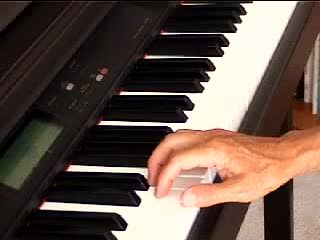
\includegraphics[height=0.4\linewidth]{TOscale.jpg}}{VPlayer.swf}
\end{center}

\subsubsection{Nácvik Palec Cez: Rýchlosť, glissandový pohyb}

\subsubsection{Stupnice: pôvod, názvoslovie a prstoklady}

\textbf{Tabuľka 1.III.5.a Vzostupne Major Váhy}\\
\noindent\begin{tabular}{L{1in}L{1in}L{1in}L{1in}}
\textbf{PR} & \textbf{ĽR} & \textbf{Stupnica} & \textbf{Krížiky/bé}\\
S1=12312341 & S2=54321321 & C,G,D,A,E & 0,1,2,3,4 krížikov\\
S1 & 43214321321 & H & 5 krížikov\\
12341231 & S2 & F & 1 bé\\
41231234 & 32143213 & b & 2 bé\\
31234123 & 32143213 & Es & 3 bé\\
34123123 & 32143213 & As & 4 bé\\
23123412 & 32143213 & Des & 5 bé\\
23412312 & 43213214 & Ges & 6 bé
\end{tabular}
\bigskip

\textbf{Tabuľka 1.III.5.b Vzostupne harmonické molové stupnice}\\
\begin{tabular}{L{1in}L{1in}L{1in}L{1in}L{1in}}
S1(PR) & S2(ĽR) & A & 0 krížikov & Gis\\
S1 & S2 & E & 1 krížik & Dis\\
S1 & 43214321 & H & 2 krížiky & Ais\\
34123123 & 43213214 & Fis & 3 krížiky & Eis\\
34123123 & 32143213 & Cis & 4 krížiky & His\\
34123123 & 32143213 & Gis & 5 krížikov & Fis\\
S1 & S2 & D & 1 bé & Cis\\
S1 & S2 & G & 2 bé & Fis\\
S1 & S2 & C & 3 bé & H\\
12341231 & S2 & F & 4 bé & E\\
21231234 & 21321432 & b & 5 bé & A\\
31234123 & 21432132 & Es & 6 bé & D
\end{tabular}

\subsubsection{Rozložené akordy (Chopinova Fantaisie Impromptu, pohyb vozíkového kolesa, rozdelenie prstov)}

\subsubsection{Bodanie a ťahanie, Beethovenova sonáta mesačného svitu, 3.časť}

\subsubsection{Palec: najvšestrannejší prst}

\subsubsection{Rýchle chromatické stupnice}

\subsection{Zapamätávanie}

\subsubsection{Prečo sa učiť naspamäť?}

\subsubsection{Kto môže, čo a kedy si zapamätať}

\subsubsection{Pamätanie si a udržiavanie}

\subsubsection{Prstová pamäť}

\subsubsection{Začanie procesu zapamätávania}

\subsubsection{Posilňovanie pamäti}

\subsubsection{Hranie bez rozohrania}

\subsubsection{Pomalé hranie}

\subsubsection{Načasovanie v duchu}

\subsubsection{Vytvorenie trvalej pamäte, hra v mysli}

\paragraph{Hudobná pamäť}

\paragraph{Fotografická pamäť} 

\paragraph{Klávesová pamäť a hra v duchu} 

\paragraph{Teoretická pamäť}

\subsubsection{Udržiavanie}

\subsubsection{Hráči z listu verzus hráči spamäti}

\paragraph{Bachove 2-hlasé Invencie: č. 1, č. 8 a č. 13} 

\paragraph{Pokojné ruky:}

\paragraph{Sinfonia č 15}

\subsubsection{Pamäťová funkcia človeka; hudba = pamäťový algoritmus}

\subsubsection{Ako sa stať dobrým hráčom spamäti}

\subsubsection{Zhrnutie}

\subsection{Cvičenia}

\subsubsection{Úvod: nevyhnutné cvičenie, rozcvičenie, a kondičné cvičenia} 
\emph{Väčšina prstových cvičení nie je užitočných}, pretože majú veľa nevýhod [pozri sekciu (h)]. Môžete nimi premárniť veľa času. V prípade, že cvičenia sú pre rozvoj techniky, aby ste mohli hrať zložité skladby, potom bude čas lepšie vynaložený na priamo na cvičenie ťažkých skladieb. Väčšina cvičení sú opakujúce sa, ktoré nevyžadujú hudobný vstup, ktoré vypnú hudobný mozog. \emph{Bezmyšlienkovité cvičenie je škodlivé.} Predpokladá sa, že cvičenia zvyšujú vytrvalosť; avšak väčšina z nás má dostatok fyzickej vytrvalosti na hranie, ale nedostatočnú výdrž mozgu; preto bezmyšlienkové opakované cvičenie môže znížiť našu celkovú hudobnú vytrvalosť. Bez správneho vedenia budú študenti cvičiť tieto opakovania mechanicky, a po krátkej dobe nezískajú žiadne nové zručnosti. Je to jeden spôsob, ako vytvoriť šatníkových klaviristov, ktorí môžu cvičiť len vtedy, keď ich nikto nepočúva, pretože nikdy necvičili robenie hudby. Niektorí vynikajúci klaviristi rutinne používajú cvičenia pre zahriatie, ale tento zvyk vznikol ako výsledok (nesprávneho) skorého tréningu a koncertní klaviristi ich nepotrebujú pri ich tréningoch.

Historicky, cvičenia typu Hanon sa stali široko prijímanými z niekoľkých mylných dôvodov: (i) že technika môže byť získaná tým, že sa naučíte obmedzený počet cvičení, (ii) že hudba a technika môže byť učená oddelene, (iii) že technika vyžaduje väčšinou svalový rozvoj bez vývoja mozgu, a (iv) technika vyžaduje silu prstov. Takéto cvičenia sa stali populárnymi u mnohých učiteľov pretože, keby fungovali, študenti by sa mohli byť naučiť techniku s malým úsilím zo strany učiteľov! To nie je vina učiteľov, pretože tieto mylné predstavy boli odovzdávané z generácie na generáciu, zahŕňajúce takých slávnych učiteľov ako Czerny, Hanon, a mnoho ďalších. Skutočnosťou je, že klavírna  pedagogika kladie značné nároky, je to časovo náročná profesia založená na vedomostiach.

\emph{Ak definujeme techniku ako schopnosť hrať, potom má najmenej tri zložky.} Má zložku \textbf{vnútornej techniky}, ktorá je jednoducho vaša úroveň zručností. Mať zručnosť však neznamená, že môžete hrať. Napríklad, ak ste nehrali za niekoľko dní a prsty sú stuhnuté, pravdepodobne nebudete môcť hrať čokoľvek uspokojivo. Takže je tam aj druhá zložka, do akej miery sa prsty sú ohybné (zložka rozcvičenie prstov). K dispozícii je tiež tretia zložka, ktorá sa bude volať formovanie. Napríklad, pre človeka, ktorý rúbal obrovské stromy po celé týždne, alebo niekoho, kto nerobil celé dni nič okrem pletenia svetrov, ruky nemusia byť v stave hrať na klavíri. Ruky sa prispôsobili na inú prácu. Na druhú stranu, cvičenie každý deň najmenej tri hodiny niekoľko mesiacov umožní rukám vykonávať neuveriteľné výkony. Definovanie komponentov techniky je dôležité, pretože tieto definície umožnia identifikovať cvičenia, ktoré sú potrebné.

Vnútorná úroveň zručností a rozcvičenie rúk sú ľahko pochopiteľné, ale formovanie je zložité. Dôležitými faktormi ovládanie formovania sú dĺžka a frekvencia cvičenia a stav mozgu/nervového/svalového systému. \emph{S cieľom udržať ruky v ich najlepšom stave hrania, bude väčšina ľudí musieť hrať každý deň.} Vynechajte niekoľko málo dní cvičenia, a formovanie sa zhorší. Preto, hoci bolo inde spomenuté, že cvičenie minimálne tri dni v týždni môže priniesť významný pokrok, zjavne výsledkom nebude najlepší vplyv formovania. Formovanie má oveľa väčší vplyv, než niektorí ľudia uvedomujú. Pokročilí klaviristi si vždy plne uvedomujú formovanie, pretože to ovplyvňuje ich schopnosť hrať. To je pravdepodobne spojené s fyziologickými zmenami, ako je rozšírenie ciev a akumulácia určitých chemických látok na špecifických miestach nervového/svalového systému. Pretože úroveň zručností stúpa, tento faktor formovania sa stáva ešte dôležitejším pre riešenie ťažkého technického materiálu a vyšších hudobných pojmov, ako je farba alebo charakteristiky rôznych skladateľov.

Ťažšie pochopiteľným faktorom, ktorý ovplyvňuje formovanie je stav mozgu/nervového systému. Tak bez zjavného dôvodu, môžete mať “dobré” a “zlé” dni. To je pravdepodobne analogické k “prepadom”, ktoré postihujú atlétov. V skutočnosti “zlé dni” môžu trvať dlhšiu dobu. S vedomím tohto javu a experimentovaním, možno tento faktor do určitej miery ovládať. Hudobníci, tak ako je golfisti, atď., sa musia naučiť, ako diagnostikovať svoje vlastné problémy. Toto uvedomenie môže pomôcť lepšie sa vyrovnať psychologicky s tými “zlými” dňami. Profesionálni športovci, napríklad golfisti a tí, ktorí praktizujú meditáciu, atď. už dlho vedia, že je dôležité formovanie mysle. Objavovanie príčiny týchto zlých dňoch by bolo ešte užitočné. Jednou obyčajnou príčinou je degradácia rýchleho hrania, ktoré bolo prebrané ku koncu časti II.25. Ďalšou častou príčinou je odchýlka od základných zásad: presnosť, načasovanie, rytmus, správne hranie po umeleckej stránke, atď. Hranie príliš rýchlo alebo s prílišným prejavom môže byť škodlivé pre formovanie. To je dôvod, prečo je tak ťažké vystupovať dvakrát za sebou a je potrebné vedieť, ako “resetovať” formovanie medzi vystúpeniami. Možné riešenia sú počúvať dobrú nahrávku, požiadať o pomoc metronóm, alebo sa vrátiť k notovému zápisu. \emph{Prehranie kompozície pomaly raz pred ukončením je jedným z najúčinnejších preventívnych opatrení proti nevysvetliteľnému “zlému hraniu” tejto kompozície neskôr.} Takže formovanie závisí nielen na tom, ako často cvičíte, ale aj o tom, čo a ako cvičíte. Solídna hra v mysli môže zabrániť prepadom; prinajmenšom ju môžete použiť, aby ste vedeli, že ste v prepade formy \textit{predtým}, než to zahráte. Ešte lepšie, môžete použiť hranie v mysli na to, aby ste sa dostali von z prepadu, nastavením času, keď je váš výkon na vrchole. Všetci používame určité hranie v mysli či už o tom vieme alebo nie. Ak nechcete vedome používať hranie v mysli, potom prepady môžu prichádzať a odchádzať, zdanlivo bez dôvodu, v závislosti na stave vášho hrania v mysli. To je dôvod, prečo je pre umelcov hranie v mysli tak dôležité.

\paragraph{Rýchle vs. pomalé svaly} Pochopenie rozdielu medzi (1) ovládaním a rýchlosťou, a (2) silou prsta pre techniku, je dôležité. Všetky zväzky svalov sa skladajú prevažne z rýchlych a pomalých svalov. Pomalé svaly poskytujú silu a vytrvalosť. Rýchle svaly sú potrebné pre ovládanie a rýchlosť. V závislosti na tom, ako budete cvičiť, jedna sada rastie na úkor druhého. Je zrejmé, že pri cvičení pre techniku, chceme pestovať rýchle svaly a znížiť tie pomalé. Preto, sa \emph{vyhýbajte sa izometrickým alebo silovým typom cvičenia. Cvičte rýchle pohyby, a hneď ako je práca vykonaná, rýchlo uvoľnite svaly.} To je dôvod, prečo akýkoľvek klavirista môže predbehnúť zápasníka sumo na klaviatúre, a to aj napriek tomu, že zápasník má viac svalov. Rýchle svaly ovládajú základný rapídny úder prsta a tieto svaly sú poháňané z mozgu, ktorý bol tiež urýchlený; pozri “rýchly úder” v (i) nižšie.

Väčšina svalov, ktoré pohybujú prstami sú v predlaktí (viď Prokop). Sú niektoré správy o tom, ktoré vyhlasujú, že najdôležitejšie svaly pre hranie na klavíri sú červovitý sval (viď Jaynes) a interossei (v rukách), ale to sú menšinové pohľady, ktoré musia počkať na ďalší výskum aby nadobudli nejakú váhu. Je však jasné, že “posilňovacie prstové cvičenia”, ako sú stláčanie pružinových zariadení predávaných na tento účel, sú zlé pre techniku, najmä rýchlosť.

Výskum “klavírnych svalov” a rýchlosti mozgu sú žalostne nedostatočné. Pretože tí, ktorí navrhli cvičenia v minulosti mali malú predstavu alebo výsledky výskumu na to, čo cvičenia potrebujú dosiahnuť, väčšina z tých cvičení je len okrajovo užitočná, a to ako boli užitočné, záviselo skôr na tom, ako ste ich použili, než ich originálnym návrhom. Napríklad, hlavným cieľom väčšiny cvičení bolo vyvinúť silu prsta, čo je chybné. Ďalšie poňatím bolo to, že čím ťažšie cvičenia ste cvičili, tým vyzretejšiu techniku ste sa naučili. To samozrejme nie je pravda; jediná pravda je, že ak ste pokročilý, môžete hrať ťažký materiál. Niektoré z najjednoduchších cvičení (ako uvidíme), vás môžu naučiť najpokročilejšiu techniku, a to je druh cvičenia, ktoré je najužitočnejšie.

\subsubsection{Cvičenia paralelných sád pre vnútorný technický rozvoj}
Pre cvičenia, aby boli užitočné, musia byť schopné identifikovať slabiny a potom posilňovať tieto zručnosti. \emph{Potrebujeme kompletnú sadu cvičení a musia byť usporiadané v nejakom logickom poradí tak, že cvičenie, ktoré rieši konkrétnu potrebu možno rýchlo nájsť.} Navrhujem to, že koncept paralelnej hry poskytuje kostru pre vytváranie univerzálnej sady cvičení. \emph{Paralelné sady (PS) sú skupiny nôt, ktoré možno prehrávať súčasne, ako akord.} Ľubovoľná hudobná pasáž môže byť postavená z kombinácií PS. Samozrejme PS samotné neobsahujú úplnú sadu cvičení; spojky, opakovanie, skoky, strečing, atď., sú potrebné a sú uvedené nižšie. Zdá sa, že Louis Plaidy učil cvičenia pripomínajúce PS cvičenia v neskorom 19. storočí.

\emph{Všetky PS cvičenia sú cvičenia RZ.} Avšak, môžete ich cvičiť tiež RS, v ľubovoľnej kombinácii, dokonca aj 2 noty proti 3, atď. Najprv si vyskúšajte trochu z každého cvičenia, potom si prečítajte časť (c) o tom, ako ich používať. Nie je potrebné, cvičiť PS samé o sebe, pretože ak sa rozvinú, bude ich  nekonečné množstvo (ako by to malo byť, v prípade, že sú kompletné), takže ich nebudete cvičiť všetky. Aj tak nikdy nebudete potrebovať všetky z nich a pravdepodobne viac ako polovica je nadbytočná. Použite tieto cvičenia len v prípade potreby (\textit{stále!}), takže jediná požiadavka v tomto okamihu je, aby ste sa s nimi zoznámili, takže môžete okamžite ísť na špecifické, požadované cvičenie, keď vyvstane potreba - už viac neplytvajte časom robením zbytočných cvičení! Akonáhle je problém vyriešený pomocou konkrétneho cvičenia, nie je potrebné, aby ste ho neustále opakovali, pretože ste už získali požadované zručnosti. \emph{PS cvičenia by nemali byť cvičené každý deň, ako cvičenia od Hanona; majú byť použité pre diagnostiku problémov a ich opravy.}

\emph{PS cvičenia sú navrhnuté tak, aby otestovali vašu techniku. Začiatočník so žiadnou technikou by mal zlyhať na všetkých z nich.} Väčšina študentov nebude mať spočiatku tušenie ako ich správne hrať. Bolo by veľmi užitočné, keby vám niekto ich niekto mohol ukázať, ak ste ich nikdy predtým nerobili. Urobím videá k dispozícii, akonáhle si nájdem čas. Mierne pokročilí študenti s 2-5 rokmi lekcií by mali byť schopný hrať uspokojivo viac ako polovicu z nich. Takže tieto cvičenia poskytujú prostriedky pre meranie vášho pokroku. Sú pre úplný rozvoj techniky, preto zahŕňajú ovládanie tónu a~hudobné hranie. Pokročilí študenti ich budú stále potrebovať ale, na rozdiel od rozvíjajúcich sa študentov, ich budú potrebovať len krátko, často len na niekoľko sekúnd cvičenia a experimentovania.

\textbf{Cvičenie č. 1}\enspace Toto cvičenie učí základný pohyb, ktorý je potrebný pre všetky nasledujúce cvičenia. \emph{Zahrajte si jednu notu}, napríklad 1. prst palcom PR ako štyri opakovania: 1111. V tomto cvičení, sa učíme, ako sa opakovať jednu “vec” rýchlo; neskôr, nahradíme “vec” s PS, takže môžeme ušetriť čas tým, že hráme toľko PS, koľko je možné v krátkej dobe. Pamätajte, že jedným z dôvodov pre nácvik cvičení je ušetriť čas. Toto opakovací pohyb je potrebný vo väčšine PS cvičeniach.

Hrajte 1111 po štvoriciach rovnakou silou, alebo ako jeden 4/4 alebo 2/4 takt. Cieľom je, aby ste ich hrali tak rýchlo, ako je to možné, a to až do rýchlosti nad jednu štvoricu za sekundu, s úplnou relaxáciou. Keď môžete zahrať štvoricu k vašej spokojnosti, skúste dve: 1111,1111. Čiarka reprezentuje pauzu ľubovoľnej dĺžky, ktorá by mala byť skracovaná, ako budete postupovať. Potom reťazec troch, potom štyroch štvoríc v rýchlom slede: 1111,1111,1111,1111. Môžete úspešne “zložiť skúšku” z tohto cvičenia ak hráte asi jednu štvoricu za sekundu, 4 štvorice v rade, len krátke pauzy medzi štvoricami. Hrajte ich ticho, uvoľnene, ale nie staccato, ako je podrobnejšie vysvetlené nižšie. Ak ste prešli skúškou 4-štvoríc, mali by ste byť schopný hrať štvorice tak dlho, a tak rýchlo, ako chcete s ovládaním a bez únavy. Tento zdanlivo triviálny pohyb je oveľa dôležitejší, než sa na prvý pohľad zdá, pretože je to základ pre všetky rýchlostné pohyby ako bude zrejmé, keď prídeme na PS zahŕňajúce mnoho prstov ako sú tie, ktoré sú v rýchlom Albertiho doprovode alebo tremolách. To je dôvod, prečo venujeme tomuto cvičeniu toľko odstavcov nižšie.

Palec má štyri hlavné spôsoby, ako sa pohybovať nadol; ostatné prsty majú tri. \textbf{Prvý pohyb je pohyb prsta:} s nehybnými rukami môžete stlačiť kláves iba pohybom prsta, najmä otáčaním každého prsta v kĺbe (“kĺb palca” je v zápästí). \textbf{Druhý pohyb je pohyb zápästia:} s nehybným predlaktím a tuhými prstami, môžete stlačiť kláves len pohybom zápästia. \textbf{Tretí pohyb je pohyb ramena.} S tuhými prstami a zápästím môžete znížiť prst posunutím celého predlaktia nadol. Tento pohyb vzniká na ramene. \textbf{Štvrtý pohyb, ktorý sa vzťahuje predovšetkým k palcu je rotácia predlaktia.} Cvičte každý z týchto pohybov oddelene, čím sa eliminuje všetko napätie. Po prvé, cvičte každý pohyb pomaly, s veľkým, prehnaným pohybom. Potom zvýšte rýchlosť zmenšením pohybov. Ďalej môžete zvýšiť rýchlosť tým, že kombinujete pohyby, pretože keď ich kombinujete, budete potrebovať ešte menšie jednotlivé pohyby na dosiahnutie rovnakého poklesu klávesu.

Skúsme celú túto rutinu s palcom ako príklad. Vo všetkých z nasledujúcich bodov, natiahnite palec von pohodlne; nezastrčte ho do rúk. (1) Pohyb palcom: Používajte iba pohyb palca na hranie štvorice, pohybujúc ho hore a dole najviac ako môžete. Ruka, paže, atď. sa nepohybujú. Vzhľadom k veľkému pohybu môžete hrať len asi jednu notu za sekundu (nebojte sa ak je vaše rýchlosť je odlišná, pretože každý človek môže mať veľmi odlišné čísla – to isté platí aj pre ostatné body nižšie). Poďme tiež predpokladať, že váš maximálny pohyb palcom je asi 10 cm. Teraz posúvajte palec iba 5 cm - môžete hrať rýchlejšie! Potom skúste 3 cm, a tak ďalej, až do najmenšieho pohybu, ktorým ešte stále zahráte notu. Ako to urýchlite, začne sa budovať napätie - toto je vaša maximálna rýchlosť. Nie je potrebné cvičiť v tomto okamihu rýchlejšie. (2) Pohyb zápästia: hrajte udržiavaním palca tuhého a otočením rukou hore a dole v zápästí. Maximálny pohyb bude asi 10 cm, a ako budete znižovať tento pohyb, budete môcť zvýšiť rýchlosť. Maximálna rýchlosť, s ktorou môžete hrať s pohyb zápästia bez napätia, by mala byť približne rovnaká ako u pri pohybe palcom zvlášť. Teraz dajte dohromady pohyby (1) a (2); mali by ste byť schopný hrať rýchlejšie než je maximum každého pohybu hraného zvlášť. (3) Pohyb ramenom: držte palec a zápästie pevné a hrajte palcom len pohybom ramena hore a dole. Začnite tým, že zdvihnete palec asi 10 cm, a zvýšte rýchlosť znížením tejto vzdialenosti. Môžte znížiť napätie s bodavým pohybom ramena s každou štvoricou, pretože tým sa využívajú rôzne svaly pre každý úder nadol. Môžete tiež zdvihnúť zápästie s každou štvoricou a tým ešte ďalej znížiť napätie. (4) rotácia predlaktia: teraz udržujte všetko tuhé a hrajte palec jednoduchým otočením predlaktia. Opäť platí, otočte palec hore asi 10 cm a zahrajte notu. Zvyšujte rýchlosť znížením tejto vzdialenosti. V zásade, mali by ste byť schopný spojiť všetky štyri pohyby, a dokonca ťah ramena a zdvihnutie zápästia, aby ste hrali najrýchlejší pohyb, ktorý je v ľudských silách. Kombinovať toľko pohybov je veľmi ťažké; cvičte ich kombináciu v pároch. Niektorí sa môžu rozhodnúť, že budú závisieť hlavne od jedného pohybu, a pridajú len trochu iných.

Každá časť tela musí byť zapojená: prsty, ruky, paže, ramená, atď., nie iba prsty. To neznamená, že každá časť sa musí pohybovať o viditeľné množstvo - môžu sa javiť stacionárne, ale musia sa zúčastniť. Veľká časť “zapojenia” bude vedomá relaxácia, pretože mozog inklinuje k tomu, aby použil príliš veľa svalov aj pre najjednoduchšie úlohy. Pokúste sa izolovať iba tie svaly ktoré sú potrebné pre každý pohyb a uvoľnite všetky ostatné. Konečný pohyb môže byť taký že sa zdanlivo pohybuje iba prst. Zo vzdialenosti väčšej ako niekoľko stôp bude si len málo ľudí všimne 1mm pohyb; ak sa každá časť tela pohla menej ako jeden mm, súčet týchto pohybov môže ľahko pridať až do niekoľkých mm potrebných pre stlačenie klávesu, a to aj bez pohybu prsta.

So zvyšujúcou sa rýchlosťou opakovania prsty/ruky/paže automaticky prejdu do pozícií, ktoré sú ideálne; PS to zabezpečia. Tieto pozície sa podobajú tým, ktoré hrajú slávni klaviristi na koncerte – a predsa to je dôvod prečo môžu takto hrať. Preto je dôležité, keď sa zúčastňujete koncertov, aby ste si zobrali váš operný ďalekohľad a sledovali detaily pohybov profesionálnych klaviristov. Pre netrénovaného pozorovateľa sa pohyby koncertného klaviristu nemusia zdať ničím neobvyklým, ale ak viete o pohyboch rúk tak, ako sú vysvetlené tu, budete ich vidieť krásne vykonané.

Začiatočníci, počas svojho prvého roku, nemusia byť schopní hrať na jednu štvoricu za sekundu. Nenúťte sa cvičiť rýchlosťou ktorú nemôžete zvládnuť bez napätia. Avšak, periodické, krátke, exkurzie do svojho najrýchlejšieho hrania sú nevyhnutné na účely prieskumu. Dokonca aj študenti s viac ako piatimi rokmi lekcií nájdu niektoré z nasledujúcich cvičení ťažké. Tí, ktorí cvičia PS prvýkrát, by mali cvičiť chvíľu cvičenie č. 1, potom cvičenie č. 2 (pozri nižšie); ak sa č. 2 sa stane problematickým pri určitých rýchlostiach (únava, napätie), tieto problémy možno vyriešiť opäť cvičením cvičenia č. 1 (skúste si to; zistíte, čo mám na mysli). Potom krátko preskúmajte ostatné cvičenia, ale nie je potrebné robiť všetky teraz, pretože bude veľa príležitostí k cvičeniu, keď vznikne potreba pri cvičení s reálnou hudbou neskôr.

\emph{Cvičte cvičenie č. 1, kým všetko napätie nezmizne a môžete cítiť ako gravitácia ťahá ruku dole.} Akonáhle sa sa vytvorí napätie, nebudete môcť cítiť gravitáciu. Nesnažte sa hrať príliš veľa štvoríc naraz ak začínate strácať kontrolu. Nepokračujte v cvičení s napätím, pretože hrať s napätím sa môže rýchlo stať zvykom. Ako sa začne vytvárať napätie, štvorice sa začnú spomaľovať; preto je spomalenie známkou napätia – to je čas na to, aby ste prepli medzi rukami. Vypracujte jednu štvoricu pred pridaním ďalšej. Dôvodom pre zastavenie v štyroch štvoriciach je, že akonáhle môžete urobiť štyri, môžete zvyčajne urobiť veľký počet po sebe. Avšak, \textit{presný} počet toho, koľko je potrebné urobiť, než ich budete môcť hrať neurčitý počet za sebou, záleží na jednotlivcovi. Pokiaľ po zreťazení dvoch štvoríc dohromady môžete hrať štvorice po neurčitú dobu pri akejkoľvek rýchlosti, potom ste zložili skúšku z cvičenia č. 1 a nemusíte ho znovu cvičiť.

Počas prvých niekoľkých dní cvičenia, by mali byť určité zlepšenia \textit{počas} cvičenia, pretože sa rýchlo učíte nové pohyby a eliminujete tie zlé. Aby ste urobili ďalší pokrok, použite zlepšenie po cvičení (ZPC), pretože nakoniec nakoniec bude potrebný nárast svalov/nervov v celom tele a mozgu. Pre ZPC, namiesto toho aby ste sa tlačili do rýchlosti \textit{počas} cvičenia, počkajte na to aby si ruka automaticky vyvinula rýchlosť, keď budete cvičiť ďalší raz; to sa môže stať, keď prepnete medzi rukami, alebo keď budete cvičiť ďalší deň.

Toto je získavanie techniky, nie budovanie svalov. \emph{Technika znamená robiť hudbu a tieto cviky sú cenné pre vývoj hudobného hrania.} Netrieskajte do klavíra ako kladivo. Ak nemôžete ovládať tón jednej noty, ako ich budete môcť ovládať keď ich bude viac? Jedným z kľúčových trikov pri ovládaní tónu je cvičiť ticho. Tým, že hráte ticho dostanete sa preč z režimu cvičenia, pri ktorom úplne ignorujte charakter zvuku a BÚCHATE, len sa snažiac dosiahnuť opakovania. Zatlačte kláves úplne a držte ho na okamih dole (veľmi krátko – zlomok sekundy). \emph{Prečítajte si časť III.1 (základný úder) ktorý je povinné čítanie, predtým, ako budete robiť vážne akékoľvek PS cvičenia.}

Aby sa zvýšila rýchlosť a presnosť a pre ovládanie tónu, \emph{udržujte prst, ktorý hrá tak blízko klávesy, ako je to možné.} Ak prst nestláča počas určitej doby klávesu, stratíte nad ním kontrolu. Neodpočívajte s prstom na klávese po celú dobu, ale dotýkajte sa klávesy, tak ľahko ako môžete aby ste vedeli kde je. To bude mať za následok pridaný cit pre to, kde sú všetky ostatné klávesy, a keď príde čas, aby ste ich hrali, prsty nájdu tie správne klávesy presnejšie. \emph{Určte minimálne zdvihy klávesu potrebné pre opakovanie a cvičte s čo najmenším zdvihom klávesu ako je to možné.} Zdvih klávesu je vyšší na pianínach než na krídlach. Vyššie rýchlosti sa dosahujú s menšími zdvihmi kláves.

Experimentujte s ovládaním tónu pomocou šmýkania prsta: skúste pohyb ťahania alebo bodania. Šmýkanie zvyšuje ovládanie, pretože vytvárate malý pokles klávesu za použitia väčšieho pohybu. Výsledkom je, že akékoľvek chyby v pohybe sa znížia o pomer medzi poklesom klávesu a celkovým pohybom, čo je vždy menšie ako jedna. Preto môžete hrať rovnomernejšie a mäkšie štvorice šmýkaním než keby ste stláčali klávesu rovno nadol. Šmýkanie tiež zjednodušuje pohyb prstov, pretože prst nemá ísť rovno dole - akýkoľvek pohyb so zložkou pohybu smerujúcou nadol to bude robiť, čo zvyšuje počet možností. Palec môže byť najjednoduchší prst na kĺzanie. \emph{Hrajte špičkou palca, nie kĺbom;} To umožní palcu kĺzať sa a zvýšiť zápästie, čím sa zníži šanca ostatných prstov náhodne trafiť niektoré klávesy. Hra so špičkou palca tiež zvyšuje efektívny rozsah a rýchlosť pohybu palca; to znamená, že pre rovnaký pohyb palca, špička sa pohybuje ďalej a rýchlejšie ako kĺb. Vedieť, ako hrať s kĺzaním prstov vám umožní hrať so sebadôverou, aj keď sú klávesy klzké, alebo, ak sa zamokria od potu. \emph{Nevyviňte si závislosť na pohybe trenia klávesu na to,  aby ste zahrali noty, pretože to nie vždy bude prítomné.} Hranie so zdvihnutým zápästím spôsobí, že prsty sa budú kĺzať smerom k vám počas poklesu klávesu. S nízkym zápästím, budú mať prsty tendenciu kĺzať sa od vás, a to najmä pre prsty 2-5. Cvičte každý z týchto kĺzavých pohybov: cvičte všetkých päť prstov so zápästím hore na chvíľu; potom zápästie dole. V strednej výške zápästia sa prsty nebudú kĺzať, a to aj v prípade, že klávesy sú klzké!

Opakujte cvičenie č. 1 so všetkými prstami, jeden po druhom. Niektoré prsty (typicky, 4 a 5) môžu byť pomalšie ako ostatné. Toto je príklad toho, ako používať tieto cviky ako diagnostický nástroj na nájdenie slabých prstov.

Správna regulácia klavírnej mechaniky a ozvučenie kladiviek je rozhodujúce pre úspešnú realizáciu týchto cvičení, a to ako pre získanie nových zručností, tak aj pre zabránenie nehudobného hraniu. To je preto, že nie je možné vyrábať mäkké (alebo silné, alebo hlboké) hudobné tóny na opotrebovaných kladivkách alebo chybných mechanikách. Budete potrebovať odborné vedenie, aby ste zabránili získavaniu zlých návykov ak cvičíte na takýchto klavíroch.

\textbf{Cvičenie č.2}\enspace \emph{2-prstové cvičenia paralelných sád:} hrajte prstami 23 v PR tóny CD tak rýchlo po sebe, ako je to možné, ako príraz na notu. Myšlienka je hrať ich rapídne rýchlo, ale pod úplnou kontrolou. Je zrejmé, že sekcie I\cite{} a II\cite{} tejto knihy sú pre to potrebné. Napríklad, v prípade, PR môže urobiť jeden cvik ľahko, ale podobné cvičenie je pre ĽR ťažké, potom pomocou PR učte ĽR. Cvičte s prírazom na 2, ako aj na tretiu dobu. Keď je to uspokojivé, hrajte jednu štvoricu ako v cvičení č. 1: 23,23,23,23. Ak máte problémy s urýchlením 23 štvorice PS, hrajte dve noty spoločne ako “akord”, a cvičte akordovú štvoricu presne tak, ako ste urobili pre jednu notu v cvičení č. 1. Opäť priveďte štvorice až do rýchlosti, asi jedna štvorica za sekundu. Potom zvýšte počet štvoríc, až kým z nich môžete urobiť reťazec 4 štvoríc idúcich za sebou. Opakujte celé cvičenie s prstami 12, 34 a 45. Potom choďte nadol: 54, 43, atď. \emph{Všetky pripomienky o tom, ako cvičiť cvičenie č. 1 platia aj tu.}

V tomto a nasledujúcich cvičeniach sa komentáre z predchádzajúcich cvičení takmer vždy sa vzťahujú na nasledujúce cvičenia a nebudem ich vo všeobecnosti opakovať. Tiež uvediem zoznam len reprezentatívnych členov rodiny cvičení a nechám na čitateľovi, aby zistil všetky ostatné cvičenia z tejto rodiny. Celkový počet cvičení je oveľa väčší, než by ste si spočiatku mysleli. Okrem toho, ak sú jednotlivé cvičenia PS cvičené v kombinácii RS, počet možností je sa rýchlo stáva strašne vysokým. Pre začiatočníkov, ktorí majú ťažkosti hrať RS, tieto cvičenia môžu poskytnúť tie najlepšie spôsoby, ako precvičiť hru RS.

\NeedRevision{}\emph{Jedným z cieľov PS je naučiť mozog koncept extrémnej rýchlosti, až skoro nekonečnej.} Akonáhle si mozog zvykne na určitú maximálnu rýchlosť, všetky pomalšie rýchlosti sa stanú ľahšie vykonateľnými. Robte všetky cvičenia spočiatku iba na bielych klávesoch. Potom, čo ste cvičili na všetkých bielych klávesoch, pracujte na podobných cvičeniach, zahrňte aj čierne klávesy.

Na začiatku, môžete byť schopní hrať veľmi rýchlo 2 noty za sebou, ale s málo nezávislým ovládaním. \emph{To môžete spočiatku “oklamať” a zvýšiť rýchlosť “fázovým uzamknutím” s dvoch prstov, napríklad tým, že držíte dva prsty v pevnej polohe (zamknutá fáza, prst 3 o niečo vyššie ako prst 2) a jednoducho znížením ruky zahráte dve noty.} Jeden jednoduchý spôsob, ako to urobiť, je stočiť prst 2 niečo viac než 3. \emph{Fázový uhol je oneskorenie medzi po sebe idúcimi prstami v paralelnom hraní. Nakoniec, musíte hrať s nezávislými prstami.} Počiatočné uzamknutie fázy sa používa iba na to aby ste sa dostali až na rýchlosť rýchlo. Toto je jeden z dôvodov, prečo niektorí učitelia neučia paralelné hranie, pretože si myslia, že paralelné hra znamená zamykanie fázy, čo je zlá technika. Jedným z dôvodov tohto problému je, že po fázového zamknutom hraní obidva prsty zostávajú na klávesoch a tie dve noty sa prekrývajú. Je rovnako dôležité zdvíhať prsty v presný čas, tak isto ako keď klesajú. Pre nezávislé hranie prstami musí prvý prst stúpať v rovnakom čase ako druhý prst hrá tak, že po sebe idúce noty sú zreteľne oddelené. Preto, schopnosť hrať 23 štvorice rýchlo nestačí. Čo si vyžaduje čas na rozvoj je nezávislé ovládanie každého prsta.

Potom, čo si môžete zahrať rýchle PS uvoľnene, spomaľte a pracujte na hraní každej note správnejšie. Začiatočníci budú mať ťažkosti so zdvíhaním prstov v správny čas, aby ovládali dĺžku noty. V tomto prípade, buď počkajte na techniku ďalej aby sa ďalej rozvíjala, alebo cvičte zdvíhacie cvičenie časti (d) nižšie.

\textbf{Cvičenie č. 3}\enspace \emph{Väčšie PS:} napríklad, 123 a jej rodina, 234, atď. Opakujte všetky postupy ako v cvičení č. 2. Potom pracujte so skupinou 1234, a napokon so sadou 12345. S týmito veľkými sadami budete možno musieť mierne spomaliť rýchlosť štvoríc. \emph{Počet možných cvičení pre tieto väčšie sady je veľmi veľký.} Príraz môže byť na akejkoľvek note a môžete začínať akoukoľvek notou. Napríklad 123 môžte cvičiť ako 231 alebo 312. Pokiaľ idete nadol 321 môže byť hraná ako 213 alebo 132; všetkých šesť možností je rozdielnych, pretože zistíte, že niektoré z nich sú ľahké, ale niektoré z nich sú ťažké. Ak zahrniete variácie prírazu, je ich už 18 cvičení a to len pre len tri prsty na bielych klávesoch.

\textbf{Cvičenie č. 4}\enspace \emph{Rozšírené PS:} začnite s 2-notovými sadami 13, 24, atď. (skupina tercií). Tieto sady tiež obsahujú typy skupín ako 14 (kvarty) a 15 (kvinty a oktávy). Potom tam sú 3-notové rozšírené PS: skupiny 125, 135, 145 (kvinty a oktávy). Tu existuje niekoľko možností pre strednú notu. Potom tú rozšírené sady hrané s 12: tercie, kvarty, kvinty, atď.; Tie môžu byť hrané s použitím 13, atď.

\textbf{Cvičenie č. 5}\enspace \emph{Zložené PS:} 1.3,2.4, kde 1.3 predstavuje interval, t.j. hrané naraz CE. Potom robte skupinu 1.4,2.5. Často som zistil, že sady ktoré ľahko idú hore, ale ťažké sú hrať smerom dole, alebo naopak. Napríklad, 1.3,2.4 je pre mňa jednoduchšie ako 2.4,1.3. \emph{Tieto zložené sady budú vyžadovať trochu zručnosti.} Ak ste nemali aspoň niekoľko rokov výučby, nečakajte, že budete môcť hrať tieto s akoukoľvek zdatnosťou.

Týmto ukončíme opakovacie cvičenie štvoríc založených na cvičení č. 1. V zásade, cvičenie č. 1 až č. 5 sú iba tie cvičenia, ktoré sú potrebné, pretože je ich možné použiť ku konštrukcii PS ako budeme pojednávať nižšie. Cvičenia č. 6 a č. 7 sú príliš zložité na to, aby sa opakovali v rýchlych štvoriciach.

\textbf{Cvičenie č. 6}\enspace \emph{Komplexné PS}: sa najlepšie cvičia individuálne a nie ako rapídne hrané štvorice. Vo väčšine prípadov, mali by byť rozdelené do jednoduchších PS, ktoré môže byť vykonávané ako štvorice; aspoň spočiatku. “Striedavé sady” sú typu 1324, a “zmiešané sady” sú typu 1342, 13452, atď., ktoré miešajú striedavé aj bežných sady. Je zrejmé, že ich je veľké množstvo. \emph{Väčšinu komplexných PS, ktoré sú technicky dôležité, možno nájsť v Bachových náučných skladbách, najmä v jeho dvojhlasných Invenciách}, pozri bod III.20. To je dôvod, prečo Bachove inštruktážne skladby (na rozdiel od Hanona) sú niektoré z najlepších cvičebných skladieb pre získanie techniky.

\textbf{Cvičenie č. 7}\enspace Teraz cvičte \emph{spojené PS}; napr. 1212, ktoré obsahujú jednu alebo viac spojok. To môže byť buď trilok (CDCD) alebo beh (CDEF, použite palec nad). \emph{Teraz tieto sady nie je možné prehrať nekonečne rýchlo, pretože rýchlosť je obmedzená vašou schopnosťou pripojiť PS.} Cieľom je tu ešte stále rýchlosť -- ako rýchlo ich môžete hrať presne a uvoľnene, a koľko z nich si môžete zreťaziť dohromady. Toto je cvičenie pre naučenie sa toho, ako hrať spojovacie noty. Tie môžu byť cvičené “pridaním prekrývajúcich sa PS”: cvičte 12, potom 21, potom 121, potom 1212. Hrajte toľko nôt, koľko môžete počas jedného pohybu ruky. Napríklad, cvičte s 1212 jedným dolným pohybom ruky.

\emph{Spojené PS sú hlavnými prvkami cvičenia v Bachových dvojhlasných Invenciách.} Preto sa pozrite na tieto Invencie ako na jedny z najviac vynaliezavých a technicky dôležitých spojených PS. \emph{Ako je vysvetlené v oddiele III.19.c, je často ťažké pre študentov zapamätať si určité Bachove kompozície a hrať ich nad určitou rýchlosťou.} Toto obmedzilo popularitu hrať Bacha, a obmedzilo použitie tohto najcennejšieho zdroja pre získavanie techniky. \emph{Avšak, keď sa analyzujú z hľadiska PS a cvičia podľa metód tejto knihy, Bachove kompozície môžu byť celkom jednoduché na naučenie.} Preto táto kniha by mala výrazne zvýšiť popularitu hrať Bacha.

Takmer nekonečný počet PS cvičení, ktoré sú potrebné ukazuje, ako žalostne nedostatočné sú staršie cvičenia (napr. od Hanona - budem používať Hanona ako všeobecného zástupcu toho, čo je považované za “zlý” druh cvičenia; nemám na mysli znepokojovať neustálou kritikou Hanona, pretože jeho cvičenia \textit{môžu} pomôcť vašej technike). Je tu jedna z výhod cvičení typu Hanon, a to, že začínajú s najčastejšie sa vyskytujúcimi prstokladmi a najjednoduchšími cvičeniami; to znamená, že sú pekne usporiadané podľa priority. Avšak, šance sú takmer 100\%, že vám málo pomôžu, keď narazíte na obtiažnu pasáž v ľubovoľnej skladbe. Koncept PS nám umožňuje identifikovať najjednoduchšie možné série cvičení, ktoré tvoria kompletnejšiu sadu, ktorá bude platiť prakticky pre čokoľvek, s čím by ste mohli stretnúť. Akonáhle sa tieto cviky stanú len trochu zložitými, ich počet sa stáva obrovským. V čase, keď sa dostanete k zložitosti aj toho najjednoduchšieho Hanonovho cvičenia sa stane počet možných PS cvičení neprekonateľne veľký. Dokonca Hanon uznal túto neprimeranosť a navrhol variácie, ako sú cvičenia vo všetkých možných transpozíciách. To určite pomáha, ale stále tomu chýbajú celé kategórie cvičení, ako je cvičenie č. 1 a č. 2 (najzákladnejšie a najužitočnejšie) alebo neuveriteľné rýchlosti, ktoré možno ľahko dosiahnuť s PS cvičeniami.

Je ľahké priviesť Hanonove cvičenia až na smiešne rýchlosti za použitia metód tejto knihy. Skúste to len tak pre zábavu - rýchlo sa začnete sami seba pýtať “Prečo to robím?”, dokonca aj tie smiešne rýchlosti sa nemôžu priblížiť tomu, čo môžete ľahko dosiahnuť s PS, pretože každé Hanonovo cvičenie obsahuje aspoň jednu spojku, a preto ich nie je možné hrať nekonečne rýchlo. \emph{To je jednoznačne najväčšou výhodou PS cvičení: nie je v nich teoreticky ani prakticky žiadny rýchlostný limit, a preto umožňujú preskúmať rýchlosť v celom svojom rozsahu.}

Ako jednu ilustráciu užitočnosti týchto cvičení predpokladajme, že chcete trilok zložený zo štyroch prstov na základe cvičenia č. 5 (napr, C.E, D.F, C.E, D.F, ...). Dodržiavaním cvičení v poradí od č. 1 až č. 7 máte teraz návod krok-za-krokom na diagnostiku svojich ťažkostí a získanie tejto zručnosti. Najprv sa uistite, že vaše dvojnotové intervaly vyrovnané použitím cvičení č. 1 a č. 2 (12 a 34). Potom skúste 1.3,2 a potom 1.3,4. Keď sú tieto uspokojivé, skúste 1.3,2.4. Potom pracujte naopak: 2.4,1 a 2.4,3, a nakoniec 2.4,1.3. Zvyšok by mal byť jasný, ak ste dočítali až sem. Toto môžu byť drsné tréningy, takže nezabudnite meniť ruky často, predtým než sa objaví únava.

\emph{Je tu opäť zdôraznené to, že v tejto knihe nie je miesto pre opakujúce sa cvičenia bez rozmýšľania.} Takéto cvičenia majú ďalšiu zákernú nevýhodu. Mnoho klaviristov ich používa na “rozcvičenie sa”, a aby sa dostali sa do skvelého hracieho stavu. To môže vyvolať nesprávny dojem, že nádherný hrací stav bol dôsledkom bezduchého cvičenia. Nie nebol; hracie podmienky po rozcvičení sú  rovnaké bez ohľadu na metódu. Z tohto dôvodu sa úskaliam bezduchých cvičení dá vyhnúť použitím prospešnejších spôsobov sa rozcvičiť. Stupnice sú vhodné pre uvoľnenie prstov a arpeggia sú užitočné pre uvoľnenie zápästí. A sú užitočné pre naučenie sa niektorých veľmi základných zručností, ako sme videli v časti (5) vyššie.

\subsubsection{Ako používať cvičenia paralelných sád (Beethovenova Appassionata, 3. veta)}
\emph{PS cvičenia nie sú určené na to aby, nahradili cvičenia Hanon, Czerny, atď. alebo akýkoľvek typ cvičenia.} Filozofia tejto knihy je, že čas môže byť lepšie využitý cvičením “skutočnej” hudby ako “cvičebnej” hudby. PS cvičenia boli predstavené, pretože nie je žiadny známy rýchlejší spôsob ako získať techniku. To znamená, že technické skladby, ako sú Lisztove a Chopinove etudy alebo Bachove Invencie nie sú v tomto zmysle “cvičebná hudba”. \emph{PS cvičenia majú byť použité nasledujúcim spôsobom:}

(i) \emph{Pre diagnostické účely:} systematické prejdenie cez tieto cvičenia vám odhalí vaše silné a slabé stránky. Ešte dôležitejšie je, pre cvičenie pasáže, ktorú nemôžete hrať, PS poskytujú spôsob identifikácie problému. Pri spätnom pohľade sa zdá zrejmé, že akákoľvek snaha o zlepšenie určitého technického aspektu bude vyžadovať nejaký diagnostický nástroj. V opačnom prípade je to ako ísť do nemocnice na operáciu, bez toho, aby poznania príčiny choroby. Podľa tejto lekárskej analógie, cvičiť Hanona je ako ísť do nemocnice dostať rovnaké “univerzálne” prehliadky/procedúry, každý deň bez ohľadu na to, či pacient je vážne chorý alebo zdravý - správny prístup je dobrá diagnóza a cielená liečba iba v prípade, človek je chorý; Okrem toho, po vyliečení, nie je potrebné, aby zachovať užívanie tých istých liekov.

(ii) \emph{Pre získanie techniky:} nedostatky zistené v (i) je teraz možné opraviť pomocou rovnakých cvičení, ktoré ich diagnostikovali. V zásade tieto cvičenia nikdy neskončia, pretože horná hranica rýchlosti/techniky je neurčitá. Avšak, vo všetkej praktickosti, končia pri rýchlostiach približne jednu štvoricu za sekundu, pretože málo, ak vôbec nejaká hudba vyžaduje vyššie rýchlosti. To ukazuje krásu týchto cvičení v umožnení cvičebných rýchlostí, ktoré sú vyššie, ako je potrebné, a tým zabezpečujú osobitný náskok bezpečnosti a kontroly.

\emph{Postupy (i) a (ii) vyriešia mnoho problémov pri hraní ťažkého materiálu.} Niekoľko úspešných aplikácií na predtým “nemožné” situácie bude generovať dôveru, že nič nie je nezdolateľné, v rozumných medziach. Ako príklad uvážme jednu z najťažších pasáží tretej vety Beethovenovej Appassionaty, takt 63, sprievod ĽR k vrcholiacemu behu PR, a podobné, následné pasáže. Počúvajte nahrávky pozorne, a zistíte, že aj tí najslávnejší klaviristi majú problémy s touto ĽR a majú tendenciu ho začať pomaly a potom zrýchliť, alebo dokonca zjednodušiť si notový zápis. Tento sprievod sa skladá zo zložených PS 2.3,1.5 a 1.5,2.3, kde 1.5 je oktáva. Získanie požadovanej techniky sa jednoducho zredukuje na zdokonaľovanie týchto PS a potom ich spojenie. Pre väčšinu ľudí bude jedna z dvoch vyššie uvedených PS bude ťažká, a to je tá, ktorú je potrebné zdolať. Snaženie naučiť sa to tým, že hrá pomaly a urýchlením RS to bude trvať oveľa dlhšie, a také učenie neprináša žiadnu záruku úspechu, pretože sa stáva pretekom medzi úspechom a budovaním rýchlostného múru. Namiesto toho cvičte RZ a meňte často ruky, aby sa zabránilo stresu a únave. Tiež, cvičte ticho na začiatku, aby ste sa učili relaxáciu.

\emph{Stručne povedané, cvičenia paralelných sád tvoria jeden z hlavných pilierov metód tejto knihy.} Sú jedným z dôvodov pre tvrdenie, že nič nie je príliš ťažké hrať, ak viete, ako cvičiť. Slúžia aj ako diagnostické nástroje a ako nástroje na vývoj techniky. Prakticky všetka technika by mala byť získaná pomocou PS počas cvičenia RZ pre privedenie do rýchlosti, naučenie sa relaxácie, a získanie kontroly. Tvoria kompletnú sadu potrebných nástrojov. Na rozdiel od Hanona, a pod., môžu byť okamžite povolaný na pomoc, keď narazíte na akúkoľvek obtiažnu pasáž a umožňujú cvičiť pri akejkoľvek rýchlosti, vrátane rýchlosti vyššej ako čokoľvek, čo budete niekedy potrebovať. Sú ideálne pre nácvik toho ako hrať bez napätia a s ovládaním tónu. Najmä sú dôležité na to, aby sa ste nadobudli návyky kĺzania prstov po klávesách a cítenie kláves pred ich hraním. Kĺzanie prstov (hladenie kláves) umožňuje ovládanie tónu a cítenie kláves zvyšuje presnosť. Bez toho, aby ste rozbili obtiažnu pasáž do jednoduchých PS, je nemožné začleniť tieto dodatočné vylepšenia do vášho hrania. Teraz sa presunieme na ďalšie užitočné cvičenia.
%%%%%%%%%% \TODO{p. 135} %%%%%%%%%%%%%%%%%%%%%%%%

\subsubsection{Stupnice, rozložené akordy a nezávislosť prstov a cvičenia na zdvíhanie prstov}

\subsubsection{Hranie (širokých) akordov, cvičenia pre rozšírenie prstov a dlane}

\subsubsection{Cvičenie skokov}

\subsubsection{Strečing a ďalšie cvičenia}

\subsubsection{Problémy s Hanonovými cvičeniami}

\subsubsection{Cvičenie pre rýchlosť}

\paragraph{Rýchly úder, uvoľnenie}

\paragraph{Iné rýchlostné metódy} 

\paragraph{Rýchlostné steny} 

\subsection{Osnova (Beethovenova sonáta č.1)}

\subsection{Uhladenie skladby – eliminovanie nepodarkov}

\subsection{Studené ruky, šmykľavé (suché/potiace sa) prsty, choroby, zranenie ruky (zápästný tunel), 
poškodenie sluchu (tinnitus)}

\subsection{Hra z listu}

\subsection{Učenie sa relatívneho a absolútneho sluchu\index{absolútny sluch|textbf} (spievanie z listu, komponovanie)}

\subsection{Nahrávanie zvuku a videa vášho vlastného hrania}

\subsection{Príprava na vystúpenia a prednesy}

\subsubsection{Základy bezchybného vystúpenia}

\subsubsection{Cvičenie pre predstavenie}

\subsubsection{Nácvik po hudobnej stránke}

\subsubsection{Príležitostné predstavenia}

\subsubsection{Prípravné rutiny pre predstavenie}

\subsubsection{Počas predstavenia}

\subsubsection{Neznámy klavír}

\subsubsection{Po predstavení}

\subsection{Pôvod a ovládanie nervozity}

\subsection{Vyučovanie}

\subsubsection{Typy učiteľov}

\subsubsection{Učenie mládeže, zapojenie rodičov, hra v mysli, absolútny sluch\index{absolútny sluch|textbf}}

\paragraph{Ako učiť vaše dieťa}

\subsubsection{Zapamätávanie, čítanie, teória}

\subsubsection{Niektoré prvky hodín klavíra a zručnosti pri vystúpení}

\subsubsection{Prečo najväčší klaviristi nemohli učiť}

\subsection{Pianíno, krídlo a elektronické klavíre; kúpa a starostlivosť o ne}

\subsubsection{Krídlo, pianíno alebo elektronický klavír?}

\subsubsection{Elektronické klavíre}

\subsubsection{Pianína}

\subsubsection{Krídla}

\subsubsection{Kúpa akustického klavíra}

\subsubsection{Starostlivosť o klavír}

\subsection{Ako sa začať učiť hrať na klavír: od najmladších detí po dospelých}

\subsubsection{Potrebujem učiteľa?}

\subsubsection{Začiatočnícke knihy a rozsah klaviatúry}

\subsubsection{Začiatočníci: vek 0 až 65+}

\subsection{“Ideálna” cvičebná rutina (Bachove učenia a Invencia č. 4)}

\subsubsection{Učenie sa pravidiel}

\subsubsection{Rutina pre učenie sa novej skladby}

\subsubsection{“Normálne” cvičebné rutiny a Bachove učenia}

\subsection{Bach: najväčší skladateľ a učiteľ (15 Invencií a ich paralelné sady)}

\subsection{Psychológia klavíra}

\subsection{Zhrnutie metódy}

\section{Hudba, matematika a výskum}

\subsection{Môžeme byť všetci Mozartmi?}

\subsection{Vedecký prístup k cvičeniu na klavíri}

\subsubsection{Vedecká metóda}

\subsubsection{Princípy učenia}

\subsection{Prečo je intuícia častokrát mylná}

\subsection{Mozartov vzorec, Beethoven a teória grúp}

\subsubsection{Mozart (Eine Kleine Nachtmusik, Sonata K300)}

\subsubsection{Beethoven (5. Symfónia, Apassionata, Waldstein)}

\subsection{Výpočet rýchlosti učenia (1000krát rýchlejšie!)}

\subsection{Budúce výskumné témy}

\subsubsection{Momentum Teória momentu hry na klavír}

\subsubsection{Fyziológia techniky}

\subsubsection{Výskum mozgu, používanie podvedomia}

\subsubsection{Budúcnosť klavíra}

\subsubsection{Budúcnosť výuky}

\section{Jazz, zbierky melódií a improvizácia}

\renewcommand\thechapter{}
\renewcommand\thesection{\arabic{section}}
\renewcommand\thesubsection{\thesection.\alph{subsection}}
\renewcommand\thesubsubsection{\thesubsection.\arabic{subsubsection}}

\chapter*{Kapitola druhá: Ladenie vášho klavíra}
\addcontentsline{toc}{chapter}{Kapitola druhá: Ladenie vášho klavíra}
\setcounter{section}{0}
\section{Úvod}

\section{Chromatická stupnica a temperovanie}

\subsection{Matematika chromatickej stupnice a intervaly}

\subsection{Temperovanie, hudba, a kvintový kruh}

\subsection{Pythagorejské, rovnomerné, celotónové, a well-temperované ladenie}

\section{Ladiace nástroje}

\section{Príprava}

\section{Začíname}

\subsection{Zapojenie a manipulácia ladiacej páky}

\subsection{Nastavovanie kolíka}

\subsection{Ladenie súzvukov}

\subsection{Súhlasné chvenie}

\subsection{Urobenie toho posledného najmenšieho pohybu}

\subsection{Vyrovnávanie napätia strún}

\subsection{Kolísanie vo výškach}

\subsection{Hrmenie v base}

\subsection{Harmonické ladenie}

\subsection{Čo je natiahnutie?}

\subsection{Presnosť, presnosť, presnosť}

\section{Postupy ladenia a temperament}

\subsection{Ladenie klavíra na ladičku}

\subsection{Kirnberger II}

\section{Drobné opravy (Zvučnosť a čistenie vratidiel)}

\subsection{Rozozvučanie kladiviek}

\subsection{Čistenie vratidiel}

\chapter*{Použitá literatúra}
\addcontentsline{toc}{chapter}{Použitá literatúra}
Knihy, ktorých autori sú označení \textbf{tučným písmom} sú recenzované nižšie.
\medskip\\
\href{http://www.music.qub.ac.uk/tomita/bachbib/}{\textit{Bach Bibliography}}.\\
Bertrand, OTT., \textit{Liszt et la Pedagogie du Piano, Collection Psychology et Pedaogie de la Musique}, (1978) E. A. P. France.\\
\noindent Boissier, August., \textit{A Diary of Franz Liszt as Teacher 1831-32}, translated by Elyse Mach.\\
\textbf{Bree, Malwine}, \textit{The Leschetizky Method}, Dover, Mineola, NY, 1977.\\
\textbf{Bruser, Madeline}, \textit{The Art of Practicing}, Bell Tower, NY, 1997.\\
\textbf{Cannel, Ward, and Marx, Fred}, \textit{How to play the piano despite years of lessons}, What music is, and how to make it at home, Crown \& Bridge, NY, 1976.\\
Chan, Angela, \href{http://www.geocities.com/Paris/Metro/5453/maped.htm}{\textit{Comparative Study of the Methodologies of Three Distinguished Piano Teachers of the Nineteenth Century: Beethoven, Czerny and Liszt}}.\\
\textbf{Eigeldinger, Jean-Jacques}, \textit{Chopin, pianist and teacher as seen by his pupils}, Cambridge Univ. Press, 1986.\\
\textbf{Elson, Margaret}, \textit{Passionate Practice}, Regent Press, Oakland, CA, 2002.\\
Fay, Amy, \textit{Music Study in Germany}.\\
Fine, Larry, \textit{The Piano Book}, Brookside Press, 4th Ed., Nov. 2000.\\
\textbf{Fink, Seymour}, \textit{Mastering Piano Technique}, Amadeus Press, 1992.\\
Fischer, J. C., \textit{Piano Tuning}, Dover, N.Y., 1975.\\
\href{http://www.speech.kth.se/music/5_lectures/contents.html}{\textit{Five Lectures on the Acoustics of the Piano}}, Royal Institute of Technology Seminar, Anders Askenfelt, Ed., Stockholm, May 27, 1988.\\
\textbf{Fraser, Alan}, \textit{The Craft of Piano Playing}, Scarecrow Press, 2003.\\
\textbf{Gieseking, Walter, and Leimer, Karl}, \textit{Piano Technique}, 2 books in one, Dover, NY,1972.\\
Gilmore, Don A., \href{http://home.kc.rr.com/eromlignod/}{\textit{In Pursuit of the Self-Tuning Piano}}.\\
Howell, W. D., \textit{Professional Piano Tuning}, New Era Printing Co., Conn. 1966.\\
\textbf{Green, Barry, and Gallwey, Timothy}, \textit{The Inner Game of Music}, Doubleday, 1986.\\
\textbf{Hinson, Maurice}, \textit{Guide to the Pianist’s Repertoire}, 3rd Edition, Indiana Univ. Press, 2000.\\
\textbf{Hofman, Josef}, \textit{Piano Playing, With Piano Questions Answered}, Dover, NY, 1909.\\
Jaynes, E. T., \href{http://bayes.wustl.edu/etj/music.html}{\textit{The Physical Basis of Music}}. (Explanation of why Liszt could not teach, best description of Thumb Over method in literature.) Jorgensen, Owen H, Tuning, Michigan St. Univ. Press, 1991.\\
\textbf{Lhevine, Josef}, \textit{Basic Principles in Piano Playing}, Dover, NY, 1972.\\
\textbf{Lister-Sink, Barbara}, \href{http://www.freeingthecagedbird.com/}{\textit{Freeing The Caged Bird}}, video, 150 min., 1996, Wingsound, Winston-Salem, NC.\\
Liszt’s Teaching Bibliography:\\
Below is a list containing information on Liszt’s teachings; the contents are disappointing. Liszt’s father, Adam, did a terrific job of teaching Liszt but, after soaring to fame, Liszt only gave “master classes” to students who were already concert pianists, while complaining about the conservatories that could not teach. The few teachers who knew how to teach were the parents of Mozart, Beethoven, Chopin, Liszt, etc. That tells us something valuable. The anointed teachers: the great Masters and their students were led astray by the grandeur of “talent”, dogma, endless practice, etc., (instead of research, knowledge, documentation, empowerment, etc.) and piano pedagogy ended up in a dead end with no way out.\\
(1) \textit{Life and Liszt}, Arthur Friedheim, Taplinger, NY, 1961.\\
(2) \textit{The Piano Master Classes of Franz Liszt: 1884-1886}, Diary Notes of August Gollerich, Indiana Univ. Press, 1996.\\
(3) \textit{Living with Liszt: From the Diary of Carl Lachmund, and American Pupil of Liszt 1882-1884}, Pendragon Press, Stuyvesant, NY, 1995.\\
(4) \textit{Memories of a Musical Life}, William Mason, Century Co., NY, 1901.\\
(5) \textit{My Musical Experiences}, Bettina Walker, R. Bently \& Son, London, 1892.\\
(6) There are a diary by Lina Schmalhausen, the other articles already cited (by Amy Fay and August Boissier), and the books by Ronald Taylor and Alan Walker.\\
\textbf{Lloyd, Norman}, \textit{The Golden Encyclopedia of Music}, Golden Press, NY, 1968.\\
\textbf{Mark, Thomas}, \textit{What Every Pianist Needs To Know About The Body}, GIA Publications, Chicago, 2003.\\
\textbf{Mathieu, W. A.}, \textit{Harmonic Experience}, Inner Tradition International, Rochester, VT, 1997.\\
Moscheles, \textit{Life of Beethoven}.\\
\textbf{Neely, Blake}, \textit{How to Play from a Fake Book}, Hal Leonard, Milwaukee, WI, 1999.\\
Olson, Steve, \textit{COUNT DOWN: The Race for Beautiful Solutions at the International Mathematical Olympiad}, 2004; “Olson explains the creative thinking process of these competitors and defies the assumption that genius is born, not made, as in music.”\\
\textbf{Prokop, Richard}, \textit{Piano Power, a Breakthrough Approach to Improving your Technique}, Greenacres Press, NY., 1999.\\
Reblitz, Arthur, \textit{Piano Servicing, Tuning, and Rebuilding}, 2nd Ed., 1993.\\
\textbf{Richman, Howard}, \textit{Super Sight-Reading Secrets}, Sound Feelings Publ., 1986.\\ \textbf{Sabatella, Marc}, \textit{A Whole Approach to Jazz Improvisation}, ADG Productions,\\ Lawndale, CA, 1996.\\
\textbf{Sandor, Gyorgy}, \textit{On Piano Playing}, Schirmer Books, NY, 1995.\\
Sethares, William A., \textit{Adaptive tunings for musical scales}, J. Acoust. Soc. Am. 96(1), July, 1994, P. 10.\\
\textbf{Sherman, Russell}, \textit{Piano Pieces}, North Point Press, NY, 1997.\\
\textbf{Suzuki, Shinichi (et al)}, two books (there are more):\\
\textit{The Suzuki Concept: An Introduction to a Successful Method for Early Music Education}, Diablo Press, Berkeley, CA, 1973.\\
\textit{HOW TO TEACH SUZUKI PIANO}, Summy-Birchard, Miami, FL, 1993.\\
\textbf{Taylor, Ronald}, \textit{Franz Liszt, the Man and the Musician}, Universe Books, NY, 1986.\\
Tomita, Yo, \href{http://www.music.qub.ac.uk/ tomita/essay/inventions.html}{\textit{J. S. Bach: Inventions and Sinfonia}}, 1999.\\
\textbf{Walker, Alan}, \textit{Franz Liszt, The Virtuoso Years, 1811-1847}, Cornell Univ. Press, Ithaca, NY, 1983.\\
\textbf{Weinreich, G.}, \textit{The Coupled Motions of Piano Strings}, Scientific American, Jan., 1979, P. 118-127.\\
\textbf{Werner, Kenney}, \textit{Effortless Mastery}, Jamey Aebersold Jazz, New Albany, IN, 1996, with meditation CD.\\
\textbf{White, W. B.}, \textit{Piano Tuning and Allied Arts}, Tuners' Supply Co., Boston, Mass, 1948.\\
\textbf{Whiteside, Abby}, \textit{On Piano Playing}, 2 books in one, Amadeus Press, Portland, OR, 1997;\\
\textit{Indispensables of Piano Playing}, and \textit{Mastering the Chopin Etudes and Other Essays}.\\
\textbf{Young, Robert W.}, \textit{Inharmonicity of Plain Wire Piano Strings}, J. Acoust. Soc. Am., \textbf{24}(3), 1952.

\section*{Recenzie kníh/videí}
\addcontentsline{toc}{section}{Recenzie kníh/videí}

\subsection*{Recenzované knihy: klasická hudba}
\addcontentsline{toc}{subsection}{Recenzované knihy: klasická hudba}

\subsubsection*{Všeobecné závery z recenzovanéch kníh}
\addcontentsline{toc}{subsection}{Všeobecné závery z recenzovaných kníh}
\begin{enumerate}[(i)]
\item Za posledných 100 rokov sa klavírna literatúra vyvinula z pôvodného dôrazu na prsty a prstové cvičenia na používanie celého tela, relaxáciu, a hudobný výkon. Preto staršie publikácie majú tendenciu obsahovať pojmy, ktoré sú teraz spochybnené. To neznamená, že Mozart, Beethoven, Chopin a Liszt nemali správnu techniku; len to, že v literatúre sa zaznamenávali väčšinou ich veľké hudobné výkony, ale nie je to, čo by ste mali urobiť, aby ste sa stali takým dobrým. Stručne povedané, klavírna literatúra bola žalostne nedostatočná, a to až do modernej doby. 

\item Jeden koncept, ktorý sa nezmenil je ten, že hudobné úvahy, o tom, ako rytmus, tón, frázovanie, atď., nemožno oddeliť od techniky. Je univerzálna zhoda medzi učiteľmi, ktorí vyučujú najlepšie metódy cvičenia, že spôsobilosť hrať na klavíri nie je talent, ale sada (naučených) zručností. 

\item Takmer každá kniha sa zaoberá podmnožinou rovnakých tém; hlavné rozdiely sú v prístupe a miere detailov, ktoré každá z nich prezentuje. Takmer všetky z nich sú čiastočnými spracovaniami a sú  neúplné. Najprv pojednávajú o ľudskej mysli a anatómii a ich vzťahom ku klavíru: mentálny postoj a príprava, sedenie, držanie tela, výška lavice, úlohy paží, rúk a prstov - často s vhodnými cvikmi, a diskusiami o zraneniach. Potom koncepty techniky a muzikálnosti: dotyk, tón, palec, legato, staccato, prstoklad, stupnice, arpeggiá, oktávy, akordy, opakované noty, rýchlosť, glissando, pedál, čas cvičenia, zapamätávanie, atď. K dispozícii je prekvapivo málo literatúry o hre z listu. 

\item S niekoľkými staršími výnimkami; väčšina odrádza od používania techniky “palec pod” pre hranie stupníc; ale technika hrania palec pod je cenná pre niektoré špecifické využitia. Chopin uprednostňoval palec pod pri hraní legato, ale učil palec cez, kde to bolo technicky výhodné. 

\item Nedostatok odkazov na použitú literatúru (referencie) v mnohých knihách je odrazom skutočnosti, že metódy klavírnej výučby neboli nikdy adekvátne a dôkladne zdokumentované alebo dokonca skúmané. Každý autor v podstate musel znovu vynájsť koleso. To sa tiež odráža v konkrétnych vyučovacích metódach. Metódy klavírnej výučby boli v podstate odovzdávané ústne od učiteľa na žiaka, pripomínajúce spôsob, akým prehistorickí ľudia odovzdávali svoje ľudové a lekárske zvyky z generácie na generáciu. Táto základná chyba takmer úplne zastavila vývoj vyučovacích metód a zostali v podstate bezo zmeny na stovky rokov. Dokonca aj “akademická” práca ako Fink má len zoznam odporúčanej literatúry, a Sandor nemá vôbec žiadne odkazy, čo je neospravedlniteľné opomenutie, ktoré odráža primitívnu povahu literatúry klavírnej pedagogiky. 

Kniha od Whitesideovej bola široko uznávaná hlavne preto, že to bol prvý skutočný pokus o vedecký prístup k objavovaniu najlepších postupov cvičenia. Avšak, podľa neoficiálnych zdrojov, väčšinu jej “objavov” učil Chopin, aj keď táto informácia zrejme nebola Whitesideovej k dispozícii. Avšak, môže byť viac než len náhoda, že vo svojom učení značne používala Chopinovu hudbu. Whitesideovej kniha sklamala preto, že, aj keď robila pokusy a zdokumentovala výsledky, nepoužívala zrozumiteľnú reč a nezorganizovala svoje výsledky, a neurobila analýzy príčin a dôsledkov atď., ktoré sú potrebné pre dobrý vedecký projekt. Avšak, jej kniha bola jednou z najlepších dostupných v čase jej publikovania, kvôli podradnej kvalite všetkých ostatných. 

Veľký počet učiteľov tvrdí, že učia metódu Liszta, ale existuje len kusé a veľmi málo dokumentácie o tom, čo táto metóda je. Existuje nadbytočné množstvo literatúry, o tom ktoré miesta Liszt navštívil, koho stretol a učil, čo hral, a to aké zázračné klavírne výkony na vysúpeniach predvádzal, ale nie je prakticky žiadny záznam o tom, čo študent musí robiť, aby mohol takto hrať. Dokonca aj Liszt nebol schopný analyzovať svoju techniku; keď bol požiadaný o to, aby učil, mohol to iba ukázať na klavíri. 

\item Changova kniha je jediná, ktorá poskytuje metódy, postupy cvičenia na riešenie konkrétnych technických problémov (prekonávanie rýchlostných múrov, relaxácie, výdrž, zapamätanie, pomalé versus rýchle hranie, atď), ktoré by mali byť vyučované vo fáze začiatočník, ale boli zriedka vyučované. Ostatné knihy sa zaoberajú predovšetkým s “vyššou” úrovňou hry na klavír, ale vyzerá, že úplne ignorujú cvičenie na klavíri, takže Changova kniha zapĺňa medzeru v literatúre o učení hry na klavíri. 
\end{enumerate}

\subsubsection*{Zoznam kníh, ktoré si MUSÍTE PREČÍTAŤ a videí, ktoré MUSÍTE VIDIEŤ}
\addcontentsline{toc}{subsection}{Zoznam kníh, ktoré si MUSÍTE PREČÍTAŤ a videí, ktoré MUSÍTE VIDIEŤ}

\textbf{Zoznam kníh ktoré MUSÍTE PREČÍTAŤ (abecedne):}\\
Eigeldinger, Fink alebo Sandor, Fraser, Prokop, Richman\\
\textbf{a videí ktoré MUSÍTE VIDIEŤ:}\\
Lister-Sink.
\medskip\\
\textbf{Formát recenzie knihy:} autor, názov, rok vydania, počet strán v knihe a to, či odkazy sú citované (bibliografia). Odkazy sú údaje o tom, ako akademická je to kniha. Tieto hodnotenia sú nie sú mienené ako vyčerpávajúce; ich obsahom je hlavne to, ako relevantné sú tieto knihy pre študenta klavíra ktorého zaujíma klavírna technika. Väčšina “irelevantných” materiálov bola ignorovaná.
\medskip\\
\textbf{Bree, Malwine}, “The Leschetizky Method”. 1997 (1913), 92P., žiadne odkazy. Hoci táto kniha vyšla v roku 1997, je to znovuvydanie materiálov z roku 1913.\\
Línia učiteľov: Beethoven-Czerny-Leschetizky-Bree. Kniha cvičení na rozvoj techniky, fotky pozícií prstov. Obhajuje metódu palec pod. Cvičenia na pozíciu rúk, nezávislosť prstov, stupnice, akordy, dotyk, glissando, pedál, vystúpenie, atď., relatívne kompletné pojednanie. Dobrá kniha na čítanie po prečítaní Changovej, ukazuje konvencie prstokladu, náznaky cvičenia RZ a ploché polohy prstov a začiatky pohybu palec cez. 
\medskip\\
\textbf{Brüser}\textbf{, }\textbf{Madeline}\textbf{,} “The Art of Practicing”. 1997, 272P., odkazy a odporúčané čítania.\\\href{http://artofpracticing.com/}{http://artofpracticing.com/}\\ Zakladá na príprave mysle (meditácia) a tela (strečingové cvičenia) na základe, a potom ide k niektorým užitočným špecifikám klavírnych zručností. Množstvo klavírnej výučby je bohužiaľ redukované paralelnými  usmerneniami pre iné nástroje (väčšinou sláčikové a dychové). Hoci fyzické cvičenia (rozcvička) sú dobré, cvičenia napríklad o stupniciach nie sú užitočné. Obsahuje malé množstvo užitočných informácií.
\medskip\\
\textbf{Chang, Chuan C.,} “\href{http://www.pianopractice.org/}{Fundamentals of Piano Practice}”, 2007 viac ako 200P., priebežne aktualizované, obsahuje referencie, recenzie kníh, odkazy na web. Táto kniha bola inšpirovaná učeniami Mlle. Yvonne Combe. Línia učiteľov: Beethoven-Czerny-Liszt-Debussy (aj Longová, Cortot)-Combe. Matka Combeovej bola hlasová učiteľka a pravdepodobne dala Yvonne dobrý štart do klavíra. Yvonne študovala pod Marguerite Longovou, a vyhrala väčšinu prvých cien v hre na klavír počas štúdia na parížskom konzervatóriu. Metódy výučby na tom konzervatóriu boli do značnej miery ovplyvnené Lisztom, a “francúzskou klavírnou školou/hudbou” odráža mnoho z jeho myšlienok. Jej hlavný mentori v Paríži boli Cortot, Debussy, a Saint Saens, a jej interpretácie týchto dvoch posledne menovaných skladateľov boli bezkonkurenčné. Bola to jedna z najsľubnejších klaviristiek svojej doby, až pokým si neporanila pravú ruku pri nehode na bicykli (bola celkom atlétka), čo ukončilo jej kariéru vystupovania. Následne sa oddala výučbe, organizovaniu škôl vo Švajčiarsku a neskôr v Plainfield, NJ, USA, kde krátko na to trénovala Van Cliburna, pretože jej metódy výučby boli podobné jeho matkiným. Hoci bola hrdá na svoju líniu Beethovena, Liszta (cez Saint Saens a Debussyho), jej interpretácie Beethovena boli v tom čase neadekvátne a svojim študentom dávala cvičiť veľmi málo od Czerného. Vo veku 86 rokov stratila väčšinu svojho sluchu, ale učila až do roku jej úmrtia vo veku 96 rokov. (životopisné poznámky C.C. Changa, od neoficiálnych zdrojov; tiež pozri komentáre na strane 1.)

Changova kniha učí najzákladnejšie tréningové metódy pre získanie techniky rýchlo (cvičenie každou rukou zvlášť, útok akordu [paralelných sád], skrátenie ťažkých pasáží, zapamätanie, relaxácia, eliminovanie rýchlostných múrov, atď). Žiadna iná kniha nepojednáva o všetkých z týchto základných prvkoch potrebných k rýchlemu pokroku a správnej technike. Hranie v mysli je jednou z najdôležitejších zručností pre pokročilých klaviristov a malo by byť vyučované od prvého roka výučby. Tiež pojednáva o hre z listu, príprave pre vystúpenia, riadenie nervozity, hranie vplyvom gravitácie, ktoré cvičenia sú dobré a ktoré z nich sú zbytočné alebo škodlivé, učenie absolútneho sluchu, náčrty, atď. Má kapitolu o ladení klavírov, vysvetľuje chromatickú stupnicu a temperovanie. Prejsť na vyššie uvedenú webovú stránku kde je stiahnutie knihy zadarmo; bola preložená do niekoľkých jazykov. \textbf{MUSÍTE SI PREČÍTAŤ.}
\medskip\\
\textbf{Eigeldinger, Jean-Jacques}, “Chopin, pianist and teacher as seen by his pupils”. 1986, 324P, bibliografia. Najviac akademická a kompletná kompilácia relevantného materiálu o Chopinovi, o učení, technike, interpretácii a histórii. Kvôli nedostatku priamej dokumentácie z čias Chopina je prakticky všetok materiál neoficiálny. Napriek tomu presnosť vyzerá byť nespochybniteľná, kvôli vyčerpávajúcej dokumentácii, nedostatku zistiteľných zaujatostí a zjavnej skutočnosti, že také hlboké porozumenie by prišlo len od Chopina samotného - výsledky sú v obdivuhodnom súlade s najlepším materiálom, ktorý je v súčasnosti k dispozícii. Eigeldinger zoradil predmety do užitočných zoskupení (technika, interpretácia, citácie, anotované notové záznamy a prstoklady, Chopinov štýl). Určite by som si prial, aby tam bolo viac metód ako cvičiť, ale všetci si musíme uvedomiť, že nedostatok dokumentácie za čias Chopina malo za následok stratu veľkej časti toho, čo vyučoval. V prípade F. Liszta je situácia oveľa horšia. 

Technické učenia sú prezentované prehľadne na stranách 23-64. Tieto učenia sú takmer v úplnej zhode s tými všetkými z najlepších zdrojov, od Liszta a Whitesidovej po Fink, Sandor, Suzuki, a tejto knihy (Chang). Prezentácia je v ostrom kontraste k Whitesideovej; tu je autoritatívna (Whitesideová niekedy dodáva jej vlastné zistenia), krátka (len 41 strán v porovnaní s 350 stránok pre Whitesideovú!), organizovaná a jasná, a zároveň pokrýva podobný rozsah tém. Druhá časť, str 65-89, zahŕňa interpretáciu, a preto obsahuje oveľa menej informácií o technike, ale je rovnako informatívna ako prvá časť. Dotýka sa (veľmi!) krátko toho, ako interpretovať každú z jeho hlavných skladieb. Zvyšných 200 strán je venovaných dokumentácii, ilustráciám, Chopinovým anotáciám svojich vlastných skladieb a prstokladom a 10 stranovej “skici” základného materiálu pre výučbu začiatočníkov. 

Poznámky k technike: Chopin bol samouk; je málo známe o tom, ako sa učil v mladosti okrem toho, že sa učil od jeho matky, vynikajúcej klaviristky. Chopin neveril v dril a cvičenia (odporúčal cvičiť nie viac ako 3 hodiny/deň). Metódy Chopina nie sú až tak v rozpore s Lisztovými, ako sa môže zdať na prvý pohľad, aj keď Liszt často cvičil viac ako 10 hodín denne a odporúčal cvičenia “do vyčerpania”. Chopin, ako aj Liszt, napísali etudy; tieto a Lisztove “cvičenia” neboli bezduché opakovanie, ale špecifické metódy na získanie techniky. 

Naučte sa robiť hudbu \textit{predtým}, než sa naučíte techniku. Celé telo musí byť zapojené a využitie hmotnosti ramena (pokles vplyvom gravitácie) je kľúčovým prvkom techniky. Učil metódu palec cez (najmä keď notu, ktorú ruka prechádza je hraná na čiernej klávese!), a tiež aj palec pod, a v skutočnosti povoľoval akémukoľvek prstu sa prevaliť cez akýkoľvek iný, keď to bolo výhodné - palec nebol jediný a musel byť “voľný”. Avšak, každý prst je iný. Metóda palec cez (rovnako ako ostatné prsty) je zvlášť užitočná v dvojitých chromatických stupniciach (tercie, atď). Pre Chopina musel klavir hovoriť a spievať; pre Liszta bol orchestrom. Vzhľadom k tomu, že C dur stupnica je ťažšia, používal H dur na učenie relaxácie a legata; ironicky, je lepšie začať sa učiť hrať staccato, aby sa eliminovali ťažké problémy pri legate, aj keď nakoniec sa vždy vrátil k svojej špecialite - hraniu legato. Široké arpeggia vyžadujú pružnú ruku viac ako široký dosah. Rubato je to, kde je rytmus striktne dodržaný, zatiaľ čo čas sa požičiava a vracia v melódii. [Môj názor je, že táto definícia je často chybne citovaná a zle pochopená; len preto, že to povedal niekoľkokrát, neznamená to, že sa aplikuje na všetko. Táto definícia rubato je uplatňovaná v situácii, v ktorej hrá PR rubato, zatiaľ čo ĽR udržuje prísny čas. Chopin určite tiež povolil, aby rubato bola sloboda od prísneho tempa kvôli prejavu.] Chopin dával prednosť klavíru Pleyel, s veľmi ľahkou mechanikou. Jeho hudbu je rozhodne ťažšie hrať na moderných nástrojoch, najmä pianissimo a legato. \textbf{MUSÍTE SI PREČÍTAŤ.}
\medskip\\
\textbf{Elson, Margaret}, “Passionate practice”, 2002, 108P., niekoľko referencií. 

Napísané z pohľadu psychológa. Obsahuje veľmi málo analytických rád v oblasti technického rozvoja a metód cvičenia. Má pekné spracovanie mentálnej vizualizácie (pozri hranie v mysli v Changovej knihe). Vhodné pre tých, ktorí sa dopúšťajú psychologických chýb (kto nie?), a pokrýva správne/zlé psychické prístupy a faktory prostredia od cvičenia po vystúpenie. Vhodné pre začínajúcich študentov, ktorí nie sú oboznámení s dennými požiadavkami klaviristov alebo pre tých, ktorí nemali skúsenosti s vystupovaním. Umenie a psychológia môžu byť prekvapivo blízke - “umelecký typ” čitateľov sa môže tešiť z tejto krátkej knihy 
\medskip\\
\textbf{Fink, Seymour}, “Mastering Piano Technique”, 1992, 187P, výborný zoznam odporúčanej literatúry; k dispozícii je tiež video. 

Najviac učená zo všetkých kníh, sú tu uvedené referencie, ako sa patrí na prácu univerzitného profesora. Vedecké pojednanie používajúce správnu terminológiu (na rozdiel od Whitesideovej, ktorá si často neuvedomovala štandardnú terminológiu), ľahká na pochopenie, začína s ľudskou anatómiou a jej vzťahom ku klavíru, nasleduje zoznam pohybov zúčastňujúcich sa pri hre na klavíri, vrátane pedálu. Stupnica nesmie byť hraná metódou palec pod, ale pod palec pod je dôležitý pohyb (strana 115). Ilustruje každý pohyb a zodpovedajúce klavírne cvičenia. Dobrý popis poklesu vplyvom gravitácie. Prísne mechanický prístup, ale táto kniha kladie dôraz na produkovanie bohatšieho tónu a hranie s emóciami. Pohyby je ťažké rozlúštiť z diagramov, takže je žiaduce, aby ste si kúpili video. Musíte si prečítať buď knihu od Finka alebo Sandora; najlepšie od oboch, pretože pristupujú k podobným témam z rôznych uhlov pohľadu. Niektorí čitatelia môžu milovať jednu a nenávidieť druhú. Fink je založený na cvičeniach, Sandor je založený viac na príkladoch z klasických skladieb. 

Prvá polovica sa venuje všetkým základným pohybom a cvičeniam pre tieto pohyby. Patria medzi ne: pronácia, supinácia, abdukcia, addukcia, pozície rúk (rozšírené, dlaňová, pazúrová), údery prstami, pohyby predlaktia, ramien, lakťov (tlačenie, ťahanie, cykly), atď. Druhá časť aplikuje tieto pohyby na na príklady od slávnych klasikov, od Ravela, Debussyho, Rachmaninova po Chopina, Beethovena, Mozarta, a mnoho ďalších. \textbf{MUSÍTE SI PREČÍTAŤ} buď toto alebo Sandora. 
\medskip\\
\textbf{Fraser, Alan}, “The Craft of Piano Playing”, 2003, 431P., bibliografia. 

Obsahuje neuveriteľné množstvo informácií, z ktorých niektoré sú najpokrokovejšie, aké kde môžete nájsť, avšak knihe chýba organizovanosť, čo vás necháva zbierať útržky cenných informácií, tak ako ich vypúšťa von. Materiály sú veľmi široko založené, od učenie od Feldenkraisa po učenie vedomia a Tai Chi Chuan po Chi-kung, ale jasne pochádzajú od dobre vzdelaného koncertného klaviristu/skladateľa. Najužitočnejšie sú presné inštrukcie o špecifických technických materiáloch: Chopinov glissandový pohyb (“oddelenie” prstov), množstvo prekrývania sa nôt pri hraní legato, hranie so stranou prstov, interpretačné chyby pri inak užitočných pojmoch, ako sú váha paží, správne použitie palca, cvičenia typu útok akordu, oktávy, fortissimo, rozvoj svalu extenzora, používanie rotácie predlaktia, muzikalita: rytmus-frázovanie-orchestrácia, atď, atď. Jedinou slabinou som našiel bolo, že je tak ohromne blízko k celkovej pravde, ale ešte sa tam nie tak celkom dostal - je tu stále priestor pre zlepšenie, a čitateľ by mal pozrieť na tieto pokročilé oblasti, kde sa môžu dokonca ukrývať novšie nápady. \textbf{MUSÍTE SI PREČÍTAŤ}; v niektorých ohľadoch informatívnejšie ako ako Fink alebo Sandor.
\medskip\\
\textbf{Gieseking, Walter, a Leimer, Karl}, “Piano Technique”, 2 knihy v jednej, 1972, žiadne odkazy.

Línia výučby: Leimer-Gieseking. Prvá kniha: Gieseking, 77p. Význam počúvania, metóda “celého tela” (a la škola hmotnosti ramien), koncentrácia, precízne cvičenie, dôraz na detail. Vynikajúce pojednanie o tom, ako analyzovať kompozíciu pre jej nácvik a zapamätanie. Táto kniha je reprezentatívna ako väčšina kníh napísaných týmimto veľkými umelcami. Typické rady v oblasti techniky sú “koncentrácia, precízne cvičenie, a pozornosť k detailu bude automaticky viesť k technike” alebo "použite vaše ucho” alebo “Všetky noty akordu musia znieť spolu”, bez toho, aby dávali nejakú radu o tom, ako vlastne získať také zručnosti. 

Ďalej prejde k tomu ako cvičiť Bachovu invenciu v C dur (č. 1), 3-hlasú invenciu v C dur (č. 1) a Beethovenovu Sonátu č. 1, ale viac z pohľadu analýzy a interpretácie, než pohľadu technických zručností. Ďalej vás sprevádza prvými 3 vetami tejto sonáty, potom neberie do úvahy štvrtú najviac technicky náročný vetu ako “nepredstavujúcu žiadne nové problémy!” Všimnite si, že táto posledná veta  vyžaduje silný, ťažký, a veľmi rýchly prstoklad 5,2,4 nasledovaný palcom-cez zostupného arpeggia v ĽR a rýchle a presné veľké skoky akordov PR. To sú miesta, kde by sme sa chceli nejakú radu od Giesekinga. Changova kniha zapĺňa túto medzeru tým, že poskytuje chýbajúci návod v kapitole prvej bod III.8. Kniha stojí za prečítanie aj len pre konkrétne pokyny na vyššie uvedené skladby. 

Druhá kniha: Leimer, 56P, žiadne odkazy .. Význam rytmu, počítanie, presné načasovanie, frázovanie. Vynikajúci sekcie o pedálovaní. Obsahuje niektoré konkrétne informácie, ktoré je ťažké nájsť inde.
\medskip\\
\textbf{Green, Barry, a Gallwey, Timothy}, “Inner Game of Music”, 1986, 225P., Žiadne odkazy. 

Duševný prístup k hudbe; relaxácia, vedomie, dôvera. Takmer žiadne technické inštrukcie pre hru na klavír. Iba pre tých, ktorí si myslia, že duševný postoj je kľúčom k hraniu na klavír. Tí ktorých zaujímajú o špecifické pokyny pre cvičenie tu nájdu len málo užitočných informácií.
\medskip\\
\textbf{Hinson, Maurice}, "Guide to Pianist’s Repertoire”, 2000, 933P., rozsiahla bibliografia. 

Veľmi ucelená kompilácia klavírnych skladieb, s krátkym popisom dôležitých informácií/charakteristík každej, stupeň obtiažnosti, dostupnosť notových záznamov, užitočné odkazy pre každú skladbu, atď. Hlavná časť je “Skladatelia: sólové práce v rôznych vydaniach”, potom obsahuje veľa užitočných zoskupení: Antológie a zbierky (podľa národnosti skladateľa, súčasné, Bachovej rodiny, atď), programy vystúpení Rubinsteina, Busoniho, a Gabrilowitscha a špeciálne indexov (Skladatelia černosi, ženy skladateľky, podľa národnosti, a pod.), 
\medskip\\
\textbf{Hofman, Josef}, “Piano Playing, With Piano Questions Answered”, 1909, 183P., žiadne odkazy.

Línia výučby: Moszkowki, Rubinstein.\\
Prvá polovica sa zaoberá veľmi užitočnými všeobecnými pravidlami a druhá polovica je vo forme otázka-odpoveď. Väčšina z knihy opisuje všeobecné pojmy; nie moc detailné technické inštrukcie. Nie je to nevyhnutná kniha pre techniku, ale predstavuje pekné bočné čítanie.
\medskip\\
\textbf{Lhevine, Josef}, “Basic Principles in Piano Playing”, 1972, 48P., žiadne odkazy. 

Vynikajúce spracovanie, ako vyrobiť dobrý tón. Stručné pojednania: základné znalosti kľúčov, stupníc, atď, rytmus, tréning ucha, tiché a hlasné hranie, presnosť, staccato, legato, zapamätávanie, čas cvičenia, rýchlosť, pedál. Väčšinou povrchné - kniha je príliš krátka. Dobré všeobecné zhrnutie, ale chýbajú konkrétne údaje, a neobsahuje materiál, ktorý nemožno nájsť inde.
\medskip\\
\textbf{Lloyd, Norman}, “The Golden Encyklopedia of Music”, Golden Press, NY, 1968, 

Šikovná hudobná encyklopédia, kde môžete nájsť takmer všetko, na jednom mieste.
\medskip\\
\textbf{Mark, Thomas}, “What Every Pianist Needs to Know About the Body”, 2003, 155P, môžete zakúpiť aj spoločne s videom; žiadne odkazy alebo index, ale navrhuje prečítať 8 textov. 

Jedno z najlepších pojednaní o ľudskej anatómii a jej vzťahu k hraniu na klavíri (vlastne akejkoľvek klaviatúre), s časťou  pre organistov a zranenia/zotavenia, odborne a medicínsky/vedecky/technicky presné. Kniha nie je o technike, ale o príprave tela/ramena/ruky na techniku a zahŕňa diskusiu o prakticky všetkých kostí/svalov od hlavy až k päte. Tiež má veľa diskusií o správnych/nesprávnych spôsobov, ako hrať, ako sú napríklad správne pohyby palca, ktoré súhlasia s propagátormi “palec cez”, nebezpečenstvo zakrivených prstov (vyvráti presvedčenie, že ploché prsty spôsobujú zranenie), potreba zrýchlenia pri poklese klávesu (pokles gravitáciou), význam hmatového vedomia predného vankúšika prsta, atď.
\medskip\\
\textbf{Mathieu, W. A.}, “Harmonic Experience”, 1997, 563P., bibliografia, značne indexované. 

Pokročilá kniha o \textit{skúsenostiach} s harmóniou; Ja nemám také vzdelanie v hudobnej teórii aby som mohol skutočne zhodnotiť túto knihu, ale budem sa ňou zaoberať z pohľadu amatérskeho klaviristu, ktorý je zvedavý. Začína sa čistými ladeniami: unisono, oktáva, kvinta, atď. a ich vzťahmi k číslam 1, 2, 3, 5, a 7. Harmónie sú v skutočnosti zažívané spevom cez monotónne bzučanie nástroja, ako je napríklad indická tambura. Potom recenzuje koncept mriežky nôt pre sledovanie harmónie, a potom stupnice, od Lydiackej cez Frygickú. Je zaujímavé, ako siedma čiastočná používaná v bluesovej hudbe zapadá do tejto schémy. Väčšina knihy je venovaná nespočetným spôsobom, v ktorých rovnaké ladenie ovplyvňuje harmóniu, ktorá môže byť skvelá pre skladateľa uzavretého do tohto temperamentu, ale sklamaním pre niekoho, kto hľadá jednoduché základné princípy harmónie a harmonických postupov (ktoré striktne povedané v skutočnosti neexistujú, kvôli Pytagorovej čiarke a jej dôsledkom). Tak hudobníci nemajú inú možnosť, než skúmať, čo je možné \textit{konkrétnou} chromatickou stupnicou, a Mathieu robí skvelú prácu, preberá problémy, s ktorými sa odborníci na harmóniu stretávajú. Takže katalogizácia harmónií v tomto nedokonalom systéme sa stáva obrovskou úlohou, aj keď sa obmedzuje na rovnaké ladenie, kde si môžete založiť katalóg na rôznych čiarkach – pamätajte, že sa to robí všetko s ohľadom na to, ako to \textit{cítite} o týchto harmóniách, nie na základe počítania frekvencií. Aby som vám dal určitú predstavu o knihe:\\
“Existuje mnoho kníh, ktorými táto kniha nie je: nie je to kniha o kontrapunkte, alebo figurovanom base, alebo melodickej alebo rytmickej štruktúre, alebo vývoji kompozície, aj keď všetky tieto predmety prichádzajú do hry. Je to kniha o harmónii, ktorá si kladie za cieľ zosúladiť a ísť nad rámec, ale nie nahrádzať tradičné texty...\\
PREHĽAD TEÓRIE: Sme si vedomí, nízkych prvočíselných pomerov medzi tónmi viac než je to príjemné - sú citové rôznymi spôsobmi. Prvočísla 2, 3, 5, a 7 slúžia ako normy jednak ako dané prírodou a aj prijatím za vlastné skúsenosťou: vnútorné/prijaté za vlastné normy. Rad alikvótnych tónov je iba jedno stelesnenie tohto, nie jeho zdroj...\\
Chyby a limity teórie: “...ktokoľvek môže vytvoriť subjektívnu tautológiu. Predstava, že afektívne čiarky sú hybnou silou za harmóniou v rovnakom ladení nikdy nemôže byť objektívne preukázaná. Čo je prezentované v tejto knihe je prepracovaný, účinný systém založený na tom, čo sa domnieva, že sú jasné vnímavosti skúmajúceho...”\\
Rozhodne s tým súhlasím, že to nie je bežná učebnica harmónie pre začiatočníkov; pre to je viac praktických informácií v sekcii “Jazz, Spevníky a improvizácia”, ktorú recenzujem nižšie 
\medskip\\
\textbf{Prokop, Richard}, “Piano Power, a Breakthrough Approach to Improving your Technique”, 1999, 108P., niekoľko odkazov. 

Táto kniha je ako zhustená forma Changovej knihy. Tento klavirista, učiteľ klavíra a hudobný skladateľ odviedol vynikajúcu prácu pri skúmaní klavírnej techniky. V krátkosti pokryje techniku RZ a cvičenie po úsekoch, špecifiká relaxácie, potrebu hudobnej hry, zapamätanie a hra v mysli. Vynikajúce fotky pozície prstov/rúk a príklady toho, čo/ako vykonávať cvičenia. Význam svalu extenzora (zdvíhača prstov); presné zdvíhanie prstov (a pedálov), cvičenia pre zdvíhanie každého prsta. Dáva najlepší opis kostí, šliach a svalov prstov/ruky/paže a ako/čím   sú riadené pohyby každým z nich. Podrobná analýza výhod/nevýhod malých, stredných a veľkých rúk. Jeho použitie “viet a dôkazov” je trochu hlúpe, pretože cvičenie na klavíri nie je matematika, a táto kompaktná kniha je neúplná, chýbajú položky, ako sú palcom cez versus palec pod (venuje sa len metóde palec pod), útok akordu, arpeggia, atď, a nie je tam žiadny priestor na rozobratie každej témy dostatočne. \textbf{MUSÍTE SI PREČÍTAŤ}, pretože budete vidieť rovnaké koncepty ako v Changovej knihe, ale od iného človeka.
\medskip\\
\textbf{Richman, Howard}, “Super Sight-Reading Secrets”, 1986, 48P., žiadne odkazy. To je najlepšia kniha na čítanie z listu. Obsahuje všetky základy, ktoré sú popísané úplne detailne, naučí vás všetku správnu terminológiu a metodiky. Začína z toho, ako čítať noty, pre začiatočníka, a postupuje logicky celou cestou až po pokročilé úrovne čítania z listu; je to užitočné najmä pre začiatočníkov. Je tiež stručná, takže by ste si mali prečítať jedenkrát celú knihu pred začatím akéhokoľvek skutočného drilu/cvičenia. Začína s tým, ako psychologicky pristupovať k čítaniu. Základné komponenty čítania z listu sú výška tónu, rytmus, a prstoklad. Po vynikajúcom úvode do hudobnej notácie, sú uvedené vhodné drily. Potom je proces čítania rozdelený na jednotlivé kroky vizuálnych, nervových, svalových a sluchových procesov, ktoré začínajú ako notový zápis a končia ako hudba. Toto je nasledované cvičeniami pre učenie “orientácie na klaviatúre” (ako nájsť noty, bez toho, aby ste sa pozerali na klaviatúru) a “vizuálne vnímanie” (okamžite rozpoznávať to, čo sa má hrať). 

V závislosti na osobe, naučenie môže trvať od 3 mesiacov do 4 rokov; mali by ste cvičiť každý deň. Nakoniec, asi jedna stránka nápadov na pokročilé čítanie z listu. \textbf{MUSÍTE SI PREČÍTAŤ.}
\medskip\\
\textbf{Sandor, Gyorgy}, “On Piano Playing”, 1995, 240p, žiadne odkazy!

Línia učiteľov: Bartók-Kodály-Sandor.\\
Kompletné a akademické, ale je to najdrahšia kniha. Obsahuje väčšinu materiálu ako Fink, zdôrazňuje metódu váhy ramien. Preberá: voľný pád, stupnicu (palec-cez metóda, má najpodrobnejší popis ako hrať stupnice a arpeggia, strana 52 až 78), rotácie, staccato, ťah, pedále, tón, cvičenie, ukladanie do pamäte, výkon. Prevedie vás tým, ako sa naučiť celú Waldstein sonátu (Beethoven). 

Početné príklady o tom, ako uplatniť princípy tejto knihy v skladbách od Chopina, Bacha, Liszta, Beethovena, Haydna, Brahmsa, Schumanna, mnohými ďalšími. Táto kniha je celkom úplná; zahŕňa predmety o tom aký je vplyv hudby na emócie po diskusie o klavíri, ľudskej anatómii a základných hracích pohyboch, na vystúpenie a nahrávanie, ale mnohé veci nie sú rozoberané dostatočne podrobne. Hlavná chyba tejto knihy je absencia akýchkoľvek odkazov, čo vrhá pochybnosti o tom, či existuje dostatočný  výskum, ktorý by podporoval obsah tejto knihy. \textbf{MUSÍTE SI PREČÍTAŤ}, ale Fink vám dá podobné informácie za nižšiu cenu.
\medskip\\
\textbf{Sherman, Russell}, “Piano Pieces”, 1997, žiadne odkazy.

Skladá sa z piatich častí, ktoré sa zaoberajú hraním, učením, kultúrnymi otázky, notovými zápismi a “všetkým ostatným”. Obsah nie je usporiadaný v žiadnom konkrétnom poradí, bez reálnych riešení alebo záverov. Opisuje politiku umenia (hudby), stanoviská, rozsudky, a pozorovania, ktoré sa môžu týkať klaviristov; či neklaviristi môžu pochopiť tieto dumania je diskutabilné, ale bude to poskytovať vhľad. Pozícia pri sedení, palec slúži ako rovnováha hybnosti. Prsty = vojaci, ale telo = dodávanie zásob, podpory, nosná loď a výroba. Prsty vs. telo = tržby vs. generálny riaditeľ; takže ovládanie prstami nevedie k hudbe. Ľahké skladby sú dôležité pre naučenie sa ako robiť hudbu. Aká je hodnota učenia hry na klavír? To nie je ani finančne dobrá kariéra. Mali by ste kĺzať prstom? Čo je zapojené do krásy a charakteru zvuku klavíra? Ako dôležité sú kvalitné klavíry a dobrých ladičov? Klady a zápory súťaží (väčšinou zápory): príprava na súťaž často nie je to ako robiť hudbu a často sa stáva skôr atletickou súťažou; stojí ten stres a úsilie za to?; porota  nie je nikdy dokonalá. 

Zaoberá sa otázkami, ktorým čelia klaviristi, učitelia a rodičia, popisuje mnoho z hlavných problémov, ale predstavuje veľmi málo riešení. Táto kniha sa dotýka mnohých otázok, ale je tak bezcieľna ako jej názov. Prečítajte si to len vtedy, ak chcete mrhať časom. 
\medskip\\
\textbf{Suzuki, Shinichi (et al.)}, dve knihy (existuje ich viac)

“The Suzuki Concept: An Introduction to a Successful Method for Early Music Education”, 1973, 216P, žiadne krížové odkazy, má veľkú vynikajúcu bibliografiu. Hlavne pre výuku hry na husle od útleho veku. Jedna malá kapitola (7 strán) o metódach výučby hry na klavíri. 

“How to teach Suzuki piano”, 1993, 21P., Žiadne odkazy. Stručný, všeobecný náčrt klavíra metód Suzukiho. Metódy opísané Changovej knihe sú vo všeobecnosti v súlade s metódami, ktoré uvádza Suzuki. Nechajte dieťa počúvať; žiadny Beyer, Czerny, Hanon alebo etudy (dokonca Chopinove!); nutnosť vystúpenia; učitelia musia mať jednotné vyučovacie metódy a otvorené diskusie (výskumné skupiny); vyváženie medzi zapamätávaním a hrou z listu, ale zapamätávanie je dôležitejšie. Učiteľom sú dané malé sady s odstupňovanou hudbou, na ktorých majú založiť svoje lekcie. Suzuki je centrálne riadená škola výučby; ako taká, to má veľa výhod fakúlt na zavedených hudobných univerzitách a vysokých školách, ale akademická úroveň je všeobecne nižšia. Suzuki učitelia sú aspoň o jeden stupeň vyšší ako priemerný súkromný učiteľ, pretože musia spĺňať určité minimálne normy. Popisuje mnoho všeobecné prístupy k výučbe, ale len málo špecifiká o tom, ako cvičiť na klavír pre techniku. Klasický príklad toho, ako autoritársky systém dokáže eliminovať zlých učiteľov zavedením minimálnych noriem, ale dobrí “Suzukiho učitelia klavíra”, musia nájsť svoje vlastné materiály nad rámec toho, čo Suzuki poskytuje.
\medskip\\
\textbf{Taylor, Ronald}, “Franz Liszt, the Mand and the Musician”, Universe Books, NY, 1986, 285P., bibliografia, register. 

Životopis - ďalšie nekonečné záznamy jeho početných ľúbostných vzťahov, so žiadnou z ktorých sa neoženil (a ktoré vytvorili najmenej 3 potomkov). Zoznam hudobníkov, z ktorých sa s väčšinou stretol, je ohromujúci: Wagner, obaja Schumannovci, Paganini, Chopin, Beethoven, Schubert, Berlioz, Brahms, Salieri, atď, nehovoriac o nemenej slávnych spisovateľov, umelcov, atď, ako je to pokryté v knihe od  Walkera (nie je potrebné čítať obe knihy - čítajte Walkera, alebo túto). Zúfalo málo informácií o tom, ako Liszt učil hrať. Neznášal pozíciu ohnutých prstov pretože vyrábala suché zvuky (str. 32) a používal flexibilný systém, v ktorom sa prsty menili aby splnili každú požiadavku. Ďalšie didaktické metódy uvedené sú dobre známe litánie pedagogických nástrojov, ako je povzbudenie verzus kritika, príliš veľa pohybov tela alebo paží, atď, ktoré neriešia špecifiká technickej hry. 
\medskip\\
\textbf{Walker, Alan}, “Franz Liszt, The Virtoso Years, 1811-1847”, 1983, 481P., obsahuje odkazy.\\
Toto je prvá z 3 kníh; vzťahuje sa na obdobie Liszta od narodenia až do doby, kedy sa rozhodol prestať  robiť predstavenia, vo veku 36 rokov. Druhá kniha sa vzťahuje na roky 1848-1861, kedy sa prevažne venoval skladaniu hudby. Tretia kniha sa vzťahuje na roky 1861-1886, jeho posledné roky. Recenzujem tu iba prvú knihu. 

Liszt je známy ako najväčší klavirista všetkých čias. Preto by sme očakávali, že sa od neho naučíme čo najviac o tom, ako získať jeho techniku. Bohužiaľ, každá kniha alebo článku napísaná o Lisztovi je z tohto hľadiska absolútne sklamanie. Možno, že technika bola ako “obchodné tajomstvo” v časoch Liszta a jeho lekcie neboli nikdy zdokumentované. Paganini cvičil v úplnej tajnosti, a dokonca aj skryto ladil husle odlišne za účelom dosiahnutia výsledkov aké nemohol nikto iný. Chopin, na druhej strane, bol skladateľ a profesionálny učiteľ - to boli jeho zdroje príjmov, a sú o tom viaceré záznamy z jeho lekcií. Nárok Liszta na slávu bol na základe jeho vystúpení. Jeho úspech sa v tomto ohľade odráža v skutočnosti, že prakticky každá kniha o Lisztovi je nekonečná a opakujúca kronika jeho neuveriteľných výkonov. Toto tajomstvo by mohlo vysvetliť, prečo tak veľa klaviristov z jeho čias, ktorí tvrdia, že boli študentami Liszta napriek tomu len zriedka popisujú metódy výučby Liszta v užitočných podrobnostiach. Avšak, keď sú tieto údaje skúšané súčasnými učiteľmi “Lisztovej školy”, dochádza sa k  záveru, že sa používajú nachádzajú na použitie podobných metód (ruky zvlášť, skrátiť ťažké pasáže, útok akordu, atď). Ďalšou možnosťou je, že pojmy Lisztovej techniky išli príliš hlboko a boli zložité na to, aby boli zredukované na jednoduché analytické vysvetlenie, nápad, ktorým sa pohodlne vychvaľovali “zázračné deti” a “talent”, ktorý bol základom ich komerčného úspechu. V skutočnosti, Changova kniha ukazuje, že základné prvky sú takmer detsky jednoduché (akonáhle vám ich niekto vysvetlí), takmer ako sedliacky zdravý rozum, pre niekoho ako Liszt, a pre neho príliš zrejmé, než aby sa tým obťažoval. Môj odhad je, že on jednoducho nebol schopný preložiť, to čo bolo v jeho prstoch do systému výučby. Nech sú skutočné dôvody akékoľvek, metódy výučby Liszta neboli nikdy adekvátne zdokumentované. Jedným z dedičstva, ktoré nám Liszt zanechal, je dobre zaznamenaná skutočnosť, že druhy výkonov ktoré robil sú ľudsky možné. To je dôležité, pretože to znamená, že všetci môžeme robiť podobné veci, ak znovu objavíme, ako to robil on. Mnohí klaviristi sa majú k tomu, a ja dúfam, že moja kniha je krok správnym smerom, aby vyrobili písomnú dokumentáciu o najznámejších metódach cvičenia. 

Walkerova kniha je typická ako ďalšie knihy o Lisztovi, ktoré som čítal, a je to v podstate kronika Lisztovho života, nie je učebnica o tom, ako sa učiť hrať na klavíri. Ako taká, je to jedna z najlepších Lisztových biografií a obsahuje početné diskusie o konkrétnych skladbách s určitými klaviristickými požiadavkami a ťažkosťami. Bohužiaľ, popis nemožnej pasáže ako takej, “ktorá bola vykonaná s najväčšou ľahkosťou” nás nenaučí, ako na to. Tento nedostatok technických informácii o výuke je prekvapujúci vzhľadom k tomu, že počet bibliografie o Lisztovi presahuje cez desať tisíc! V skutočnosti, každá užitočná technická informáciu, ktorú môžeme vyčítať z tejto knihy musí byť odvodená z obsahu pomocou vlastných znalostí klavíra (pozri “relaxačný” príklad nižšie). Sekcia nazvaná “Liszt a klaviatúra” (str. 285 - 318) obsahuje niekoľko rád o tom, ako hrať. Rovnako ako vo všetkých troch knihách, Liszt je uctievaný ako poloboh, ktorý nemôže urobiť nič zlé, dokonca je obdarený super rukami nejako ideálne nastavenými pre hru na klavíri - mohol dosiahnuť ľahko interval decimy. Toto skreslenie znižuje dôveryhodnosť a neustále, opakované správy o nadľudských výkonoch vytvárajú nudnosť, ktorá odvádza pozornosť od obrovského množstva odhaľujúcich a fascinujúcich historických detailov v týchto knihách. 

Z hľadiska “neuveriteľných predstavení”, ktoré viedli na polámané struny, je snáď zaujímavé, že Liszt bol chudý, fyzicky slabý muž v ranej mladosti. Vo veku troch rokov, sa ho vzdali po chorobe, a dokonca mu objednali rakvu. Začal hrať na klavíri niekedy pred vekom šiestich rokov, a nemal ani v prijateľné cvičenie na klavíri až do siedmich rokov, pretože jeho rodina bola tak chudobná. Učil ho jeho otec, talentovaný muzikant, slušný klavirista a blízka známosť Haydna, a bol ponorený do hudby už od narodenia. A predsa, v siedmich rokoch bol “privádzal do úžasu svojich rodičov hrou na klavíri a už v tom veku komponoval”. Tieto správy nie sú spravodlivé k jeho otcovi, ktorý pravdepodobne najviac vplýval na rapídny rozvoj Liszta. Czerny bol jeho prvý “skutočný” učiteľ, vo veku 11 rokov (Czerny poznamenáva, že Franz ani nevie, správne prstoklady), a Czerny tvrdí, že naučil Franza všetky jeho základné zručnosti. Avšak, on uznáva, že Franz bol už zrejmý zázrak, keď mu ho predstavili (vedel hrať z listu prakticky čokoľvek) - čo sa zdá podozrivo nekonzistentné. Franz sa v skutočnosti búril proti drilom Czernyho, ale napriek tomu značne používal cvičenia k jeho technickému vývoju a vyjadril najvyššiu úctu svojmu učiteľovi, tak ako aj Beethoven. Veci, ktoré cvičil boli základy: behy, skoky, opakované noty. Moja interpretácie je, že to neboli len bezduché opakovania pre budovanie svalov, ale cvičenia na získanie šikovnosti, ktoré mali na mysli špecifické ciele, a akonáhle bol cieľ dosiahnutý, presunul sa na niečo nové. 

Ale ako môže krehká osoba vykonávať “nemožné” cvičenia do vyčerpania? Tým, že relaxuje! Liszt môže byť najväčší svetový expert na relaxáciu, z nutnosti. Pokiaľ ide o relaxáciu, môže to byť náhoda, že Paganini bol tiež chorý človek. V čase, keď sa stal slávnym, po tridsiatke, Paganini mal syfilis, a jeho zdravotný stav ešte zhoršil kvôli závislosti na hazardných hrách a kontrakcie tuberkulózy. Napriek tomu, títo dvaja muži zlom zdravotnom stave boli dvaja najväčší majstri ich nástrojov (ako dospelý bol Liszt bol pomerne zdravé vzhľadom na jeho dobu). Skutočnosť, že obaja neboli fyzicky robustný znamená, že energia pre nadľudské výkony nepochádza z atletickej svalovej sily, ale skôr od úplného ovládnutia relaxácie. Chopin bol tiež na strane krehkého, s tuberkulózu. Smutná historická poznámka, okrem Paganiniho zlého zdravotného stavu a groteskných dôsledkov primitívnych chirurgických pokusov tej doby, sú jeho okolnosti príšernej smrti, pretože pri jeho pohrebe bolo oneskorenie, a bol ponechaný na hnitie v nádrži s betónom. 

Ďalší pozoruhodný učiteľ Liszta bol Salieri ktorý ho učil kompozíciu a teóriu. Salieri učil tiež Schuberta, ale Liszt sa s ním nikdy nestretol. V tej dobe mal Salieri cez 70 rokov, trpel pre podozrenie z otrávenia Mozarta zo žiarlivosti. Liszt sa stále zlepšoval vo veku 19 rokov. Jeho výkony sú pripočítaný k popularizácii klavíra. Je mu pripisované vynájdenie klavírneho recitálu (tým, že ho preniesol zo salónu do koncertnej sály). Jeden z jeho zariadení bolo použitie mnohých klavírov, rovnako ako mnoho klaviristov. Dokonca hral klavírne koncerty pre viac klavírov so Chopinom a ďalšími osobnosťami svojej doby. To vyvrcholilo oslavami až so šiestimi klavírmi, s reklamou ako “koncert 60 prstov”. V jednom úseku 10 týždňov, hral 21 koncertov a 80 diel, 50 spamäti. To, že tak mohol okúzliť svoje publikum bolo viac prekvapujúce, pretože zodpovedajúce klavíre (Steinway, Bechstein) neboli k dispozícii až do roku 1860, takmer 20 rokov po tom, čo prestal koncertovať.
\medskip\\
\textbf{Whiteside, Abby}\textbf{,} “On Piano Playing”, 2 knihy v jednej, 1997 , žiadne odkazy. Jedná sa o znovuvydanie “Indispensables of Piano Playing” (1955), a “Mastering Chopin Etudes and Other Essays” (1969). Výučba riadkov: Ganz - Whitesideová. 

\textbf{Prvá kniha:} “Indispensables of Piano Playing”, 155P. Používa neštandardnú angličtinu, spletitú logiku, biblické frazeológiu, dlhé rozvláčne a opakujúce sa. 

Obsah je vynikajúci, ale je to hrozné spísané a to robí učenie neproduktívnym. Mnohé z nápadov, ktoré opisuje sú v iných knihách, ale ona mohla sama objaviť (alebo znovuobjaviť) väčšinu z nich. Aj keď som mal problémy s čítaním tejto knihy, iní tvrdia, že je ľahšie ju pochopiť, ak ju viete prečítať rýchlo. To je preto, že často jej treba odsek alebo dokonca stránku na popísanie niečoho, čo môže byť zapísané v jednej vete. 

Takmer celá kniha je ako toto (str. 54): “Otázka: Môže Hmotnosť - meravý tlak - prispievať k rozvoju ovládania hry. Odpoveď: Je to presne ten meravý tlak hmotnosti, ktorý nemôže byť použitý pre rýchlosť. Slová sú dôležité vo výučbe. Slová činu sú potrebné aby navrhli opatrenia pre koordináciu rýchlosti. Hmotnosť nenasvedčuje aktivite svalov, ktorá sa pohybuje hmotnosťou ramena. Toto naznačuje meravý tlak.” Nevybral som si túto časť, pretože bola mimoriadne spletitá - bola vybraná náhodne otvorením knihy so zavretými očami. 

Obsah: Musíte nasledovať jej metódy nábožensky; prečo je rytmus dôležitý, kombinácia tela-paží-rúk-prstov má nekonečné možnosti, ktoré si väčšinou neuvedomujeme; stupnica hraná metódou palec pod je preklínaná; funkcie každej časti tela pre hranie na klavíri (horizontálne, vnútorné-vonkajšie, vertikálne pohyby); diskusie o vytváraní emócií, zapamätanie, pedálovanie, frázovanie, trilky, stupnice, oktávy, vyučovacie metódy. Poukazuje na význam rytmu hudby a ako dosiahnuť to pomocou náčrtov (s. 141). Czerny a Hanon sú k ničomu, alebo ešte niečo horšie. 

Toto je jej útok na podkladanie palec-pod pre hranie stupnice, výňatok z viac ako dvoch strán, () sú moje vysvetlenia: 

\textit{“Podkladanie.} Tu sa stretávame s množstvom stresu v tradičnej výučbe ktorá sa zaoberá presnými pohybmi, ktoré by mali byť vykonávané s prstom a palcom ... Keby sme mohli odstreliť tieto pojmy priamo z existencie ja by som neváhala, aby sa tak urobilo. Toto je to, aké chybné a zhubné si myslím, že sú. Môžu doslova ochromiť klaviristu... Ak to (hranie perfektných stupníc) vyzerá celkom beznádejne nemožné, a nemáte záblesk nápadu, ako to možno dosiahnuť, potom sa snažíte s koordináciou, ktorá vlastne robí stupnicu nemožnú zahrať. To znamená, že sa palec podkladá pod dlaň aby dosiahol pozíciu; a prsty sa snažia dostať cez palec a hľadám legato pripojenie kľúčovú Nezáleží na tom, či umelec dosiahnutie rýchle a krásne váhy a arpeggia vám povie, že robí len to (palec pod) - to nie je pravda, žiadne návrh znamená, že klame, ale len to, že bol úspešný v likvidácii koordinácie, ktorý sa učil, keď. príležitosti vznikol ktorý robil to neadekvátne .... Oni (palec pod hráčov) musí byť znovu vzdelaný fyzicky na nový model koordinácie, a že prevýchova môže znamenať obdobie katastrofálne biedy k nim ..... . účinkom (palcom po prechode) môžu byť prijaté pomocou ramenného kĺbu v ľubovoľnom smere. horné rameno môže pohybovať tak, že koniec koleno humeru môžete popísať segment kruhu, hore alebo dolu, dovnútra a von, tam a ďalej, alebo okolo a okolo .. (atď, celá stránka tohto typu výučby o tom, ako hrať palcom) ..... S ovládaním od centra celý koordinácia funguje, aby bolo jednoduché mať prst k dispozícii na adrese v okamihu, kedy je to potrebné .... Najlepším dôkazom tohto tvrdenia je krásna stupnica alebo arpeggio hrané s úplnou ľahostajnosťou k akémukoľvek konvenčnému prstokladu. To sa často deje u nadaného, nevzdelaného klaviristu... Pre úspešné absolvovanie (palcom), horné rameno slúži ako opora pre všetky “iné techniky” zahŕňajú predlaktia a ruky, flexia a extenzia v lakti, rotačné akciu, a postranné ručný zásah na zápästie, a posledná a najmenšia, bočné akciu prstov a palca .... . Medzi rotačné akcie a striedavého pôsobenia, absolvovaní je tak jednoduché, ako to vyzerá, keď to robí odborník.” 

\textbf{Druhá kniha:} “Mastering the Chopin Etudes and Other Essays”, 206P, žiadne odkazy. 

Kompendium redigovaných rukopisov Whitesideovej; oveľa čitateľnejšie, pretože bolo upravované jej študentami, a obsahuje väčšinu z myšlienok prvej knihy, založené na hraní Chopinových etúd, ktoré boli vybrané pre svoj neprekonateľný hudobný obsah, rovnako ako pre ich technickú výzvu. To je ako katechizmus pre vyššie uvedenú bibliu; môže byť dobrým nápadom, aby ste si túto knihu prečítali pre prvou knihou. Celkom podrobne popisuje ako urobiť náčrt diela: strana 54 až 61 základný popis a str.191-193 základná definícia, s viacerými príkladmi na str.105-107 a str. 193-196. Hoci načrtávanie môže byť použité na odstránenie technických ťažkostí, je cennejšie pre učenie, alebo učenie ako hrať, hudobného konceptu kompozície. 

Tieto dve knihy \textit{sú} diamantovou baňou praktických nápadov; ale ako diamantová baňa, musíte siahnuť hlboko a nikdy neviete, kde sú diamanty zakopané. Použitie Chopinových etúd sa tu ukáže, že sa nejedná o náhodný výber, väčšinu základných princípov Whitesideovej učil už Chopin (pozri knihu od Eigeldingera), ale Eigeldingerova kniha bola napísaná dlho po Whitesideovej knihe a ona zrejme nevedela veľa o Chopinovej metóde. 

Neexistuje žiadna stredná cesta - budete buď milovať Whitesideovú pre jej poklad informácií alebo nenávidieť, pretože je nečitateľná, opakujúca sa a neorganizovaná.

\textbf{Weinreich, G.} “The Coupled Motions of Piano Strings”, Scientific American, Jan. 1979, P. 118-127. 

Toto je dobrý článok o pohyboch klavírnych strún, ak sa potrebujete naučiť samotné základy. Avšak, tento článok nie je dobre napísaný a experimenty neboli dobre urobené; ale mali by sme byť vedomí obmedzených zdrojov, ktoré autor zrejme mal. Isto bol dlho pred rokom 1979 vykonaný pokročilejší výskum výrobcami klavírov a vedcami z oblasti akustiky. Budem tu recenzovať niektoré nedostatky, ktoré som našiel v tomto článku v nádeji, že povedomie o týchto nedostatkoch umožní čitateľovi zbierať ďalšie užitočné informácie z tejto publikácie, a aby sa  vyhol tomu, aby bol uvedený do omylu. 

Nie sú tu vôbec žiadne informácie o špecifických frekvenciách tých nôt, ktoré boli skúmané. Vzhľadom k tomu že správanie klavírnych strún je tak závislé na frekvencii, je to zásadná informácia, ktorá tu chýba. Majte to na pamäti, až budete čítať tento článok, ako veľa výsledkov bude ťažké interpretovať, bez toho aby vedel frekvenciu, pri ktorej boli experimenty vykonávané, a preto sa stal pochybné hodnoty. Napríklad rôzne experimenty boli vykonané na rôznych frekvenciách, v takom prípade by sme vedieť, ako sa ich porovnanie. 

Stredný graf v dolnom rade obrázkov na str. 121 (v tomto článku nie sú žiadne čísla obrázkov!) nie je dostatočne vysvetlený. V článku neskôr autor navrhuje, že vertikálne režimy produkujú okamžite znejúci zvuk. Obrázok preto môže byť interpretovaný ako ukázanie zadržania jednej struny. Neviem o žiadnej pedálovanej note na klavíri, ktorý by mala zadržanie struny kratšie ako 5 sekúnd, ako naznačuje obrázok. Obrázok vľavo v hornom rade grafov pre jednu strunu ukazuje držanie tónu na viac ako 15 sekúnd, čo súhlasí s mojimi zbežnými meraniami na skutočnom krídle. Z toho vyplýva že grafy týchto jediných strún sa zdajú byť v rozpore. Na hornom grafe bol meraný akustický tlak, zatiaľ čo na dolnom posun struny, takže nemusí byť striktne porovnateľné, ale my by sme si priali keby autor poskytol aspoň nejaké vysvetlenie tohto zdanlivého rozporu. Pre tieto dva obrázku mohli byť použité struny s veľmi rozdielnymi frekvenciami. 

Vo vzťahu k týmto obrázkom, je tu táto veta: “Použil som citlivú elektronickú sondu, aby som samostatne odmeral vertikálne a horizontálne posuny jednej struny,” bez akýchkoľvek ďalších informácií. V tomto okamihy by akákoľvek vedca v tejto oblasti veľmi zaujímalo, ako to autor urobil. V riadnej vedeckej správe, to je normálný (obvykle \textit{vyžadovaným)} postupom identifikácia zariadenia (obvykle vrátane čísla výrobcu a modelu), a dokonca to, ako bolo obsluhované. Výsledné údaje sú jedny z mála nových informácií uvedených v tomto dokumente, a sú preto v tomto článku nanajvýš dôležité. Budúci bádatelia budú pravdepodobne musieť nasledovať postup po tejto línii štúdie merania posuny struny detailnejšie a budú potrebovať informácie o prístrojoch. 

Na štyri obrázky na strane 122 sa auto neodvoláva nikde v článku. Tak to je ponechané na čitateľoch hádať, v ktorá časť článku sa ich týka. Taktiež môj odhad je, že spodné dva grafy ukazujúce oscilácie sú len schémy a nepredstavujú nič, čo by sa približovalo skutočným údajom. V opačnom prípade, by bol okamžite znejúci zvuk by sa ukončil v priebehu asi 1/40 sekundy, podľa týchto grafov. Krivky zakreslené v týchto dvoch spodných obrázkoch sú čisto imaginárne okrem toho, že sú schematické. K dispozícii nie sú žiadne údaje ktoré by ich podložili. V skutočnosti článok nepredstavuje žiadne ďalšie nové údaje a diskusia na nasledujúcich 5 stranách (z 8 stránok článku) je v podstate prehľadom známych akustických princípov. Ako také, popisy pružných, masívnych a odporových ukončení tónu, ako aj rezonančných vibrácií, by mali byť kvalitatívne platné. 

Hlavnou tézou tohto článku je, že klavír je jedinečný, pretože má dozvuk a správne vyladenie dozvuku je podstatou dobrého ladenia a vytvára jedinečnú klavírnu hudbu. Pre mňa ťažkosťou tejto tézy je, že dozvuk zvyčajne trvá po dobu 5 sekúnd. Len veľmi málo klavírnych nôt je hraných tak dlho. Preto v podstate všetka klavírna hudba sa hrá iba pomocou okamžite znejúceho zvuku. V skutočnosti, klavírni ladiči používajú predovšetkým okamžitý zvuk (ako je tu definované) pri ladení. Okrem toho, dozvuk má  aspoň o 30dB menej energie; výsledok je len niekoľko percent pôvodného zvuku. To bude úplne prehlušené  všetkými ostatnými notami v každej skladbe. Čo sa deje v skutočnosti je, že nech čokoľvek čo riadi kvalitu zvuku klavíra, riadi aj okamžitý zvuk a aj dozvuk, a to čo potrebujeme, je pojednanie, ktoré vrhá svetlo na tento mechanizmus. 

A konečne, potrebujeme publikáciu so správnymi odkazmi na literatúru, takže môžeme vedieť, čo bolo alebo nebolo doteraz skúmané (na obranu autora, Scientific American nepovoľuje žiadne iné odkazy, s výnimkou odkazov na už skôr publikované články v časopise Scientific American. Preto je nutné, písať články, ktoré sú “sebestačné”, ktorým tento článok nie je. Podľa Reblitza [str. 14], existuje článok z roku 1965 v Scientific American o “The Physics of the Piano”, ale na tento článok sa v tomto neodkazuje). 
\medskip\\
\textbf{\href{http://www.speech.kth.se/music/5_lectures/contents.html}{Five Lectures on the Acoustics of the Piano}}, seminár na Royal Institute of Technology, Anders Askenfelt, Ed., Štokholm 27. mája 1988. 

Niektoré z najvyspelejších sérií prednášok o tom, ako klavír produkuje zvuk. Úvod je o histórii klavíra a informáciách o terminológii a znalostiach nevyhnutných pre pochopenie prednášok. 

Prvá prednáška sa zaoberá konštrukčnými faktormi klavíra, ktoré majú vplyv na tón a akustický výkon. Kladivká, zvuková doska, puzdro, rám, struny, ladiace kolíky, a ako spolu pracujú. Ladiči ladia priečne vibračné režimy strún, ale pozdĺžne módy sú pevne stanovené strunou a návrhom stupnice a nemôže byť riadený ladičom, napriek tomu má počuteľné efekty. 

Druhá prednáška je zameraná na klavírny tón. Kladivko má dva režimy ohýbania, režim ohnutia stopky a rýchlejší vibračný režim. Prvým z nich je spôsobený rapídnym zrýchlením kladivka, podobne ako ohnutie golfovej palice. Druhý je najvýraznejší, keď sa kladivo odrazí späť od strún, ale môže byť tiež vybudený počas svojej cesty k strunám. Je zrejmé, že tlmič je dôležitým prvkom, ktorý klavirista môže použiť na zníženie alebo kontrolu týchto vedľajších pohyby kladivka, a tým kontrolovať tón. Skutočný od času závisiaci pohyb struny je úplne rozdielny od pohybu vibrujúcich strún uvedených v základných učebniciach fyziky a harmonickými zložkami, ktoré sú neoddeliteľnými zlomkami vlnovej dĺžky, ktoré sa ľahko zmestia medzi fixované konce strún. Je to vlastne sada šíriacich sa vĺn tam a späť spustených kladivkom smerom k mostíku a smerom k agraffe. Tieto sa šíria tak rýchlo, že kladivko je “prilepené” na struny pre niekoľko málo prechodov týchto šíriacich sa vĺn sem a tam, a to je sila jednej z týchto vĺn ktorá nakoniec hádže kladivko späť k tlmiču. Potom ako je možné, že sa vytvorí hlavná a vyššie harmonické zložky? Jednoducho - sú to len komponenty Fourierovej šíriacich sa vĺn! V nematematických pojmoch, to znamená že jedinými šíriacimi sa vlnami možnými v tomto systéme sú vlny, ktoré majú uzly na oboch koncoch, pretože systém je obmedzený pevnými koncami. Držanie tónu a rozdelenie harmonických zložiek je veľmi citlivé na presné vlastnosti kladivka, ako je veľkosť, hmotnosť, tvar, tvrdosť, atď. 

Struny prenesú svoje vibrácie na rezonančnej dosky (RD), cez mostík a účinnosť tohto procesu môže byť stanovená meraním zhody akustickej impedancie. Tento prenos energie sa komplikuje rezonanciou v RD vyrobenej normálnych režimov vibrácií, pretože rezonancie produkujú vrcholy a údolia na krivke impedancia/frekvencia. Účinnosť výroby zvuku je nízka pri nízkej frekvencii, pretože vzduch môže znamenať “záverečný beh” vnútri klavíra tak, že tlaková vlna nad RD môže zrušiť vákuum pod ňou, keď vibruje smerom nahor (a naopak pri pohybe nadol). Pri vysokej frekvencii vibrácie RD vytvárajú mnoho malých plôch pohybujúcich sa v opačných smeroch. Vzhľadom k ich blízkosti, môže stlačený vzduch v jednej oblasti zrušiť susedné oblasti vákua, čo má za následok menej zvuku. To vysvetľuje, prečo malé zvýšenie veľkosti klavíra môže výrazne zvýšiť zvukovú produkciu, a to najmä pre nízke frekvencie. Tieto komplikácie jasné poukazujú na to, že zosúladiť akustické impedancie naprieč všetkých tónov klavíra je monumentálna úloha, a vysvetľuje, prečo dobré klavíry sú tak drahé. 

Vyššie uvedené je môj pokus o stručný preklad vysoko technického materiálu, a pravdepodobne nie je 100\% správny. Mojím hlavným cieľom je poskytnúť čitateľovi určitú predstavu o obsahu prednášok. Je zrejmé, že táto webová stránka obsahuje veľmi náučný materiál. 

\subsection*{Recenzované knihy: Jazz, zbierky melódií a improvizácia}
\addcontentsline{toc}{subsection}{Recenzované knihy: Jazz, zbierky melódií a improvizácia}
\textbf{Cannel, Ward a Marx, Fred}, “How to play the Piano despite Years of Lessons”, What music is, a nd how to make it at home, 239P., 1976, žiadne odkazy. 

Začína kritizovaním mylných predstáv o talente, opakovaných cvičeniach, nadradenosti klasickej hudby, atď, ktoré odrádzajú ľudí od toho aby sa z nich stali hudobníci. Skvelá kniha pre začiatočníkov, počnúc od najzákladnejšie informácií, hrania jednonotových melódií, atď. Naučíte sa hrať melódie/skladby od samého začiatku. Jednou z hlavných chýb je - nie sú uvedené prstoklady k akejkoľvek skladbe v celej knihe! Potom sa základné akordy (3 notové), potom “kostra”, univerzálna schéma melódie pre PR melódie a sprievodu pre ĽR, ktorá vám umožní hrať takmer čokoľvek. Potom 4-notové akordy, rytmus (dôležité!), arpeggiá. Bolero (Rumba, beguine, calypso), tango, shuffle. Kvintový kruh a postupy akordov: klasický, romantický, impresionistický, moderný - veľmi praktické a užitočné. Hra podľa sluchu, improvizácie. Ako zakončiť akýkoľvek skladbu. Dobre navrhnuté sekvencie od veľmi jednoduchých až po zložitejšie pojmy, vedie vás cez ne najjednoduchšou možnou cestou. Doplnok s 29 populárnymi piesňami na cvičenie a učenie sa z nich (gitarové a organové značky, meniace sa aranžmány počas behu, ako robiť veci ešte zaujímavejšími, atď). Kniha je plná ľahko pochopiteľných vysvetlení základných pojmov a užitočných trikov. Táto kniha nie je pre tých, ktorí chcú získať techniku a hrať ťažké skladby.
\medskip\\
\textbf{Neely, Blake}, “How to play from a Fake Book”, 87P, 1999; žiadne odkazy, ale má dobrý zoznam spevníkov. 

Výborná kniha na začiatok; spevníky sú jednoduché, pretože sa nemusíte učiť postupnosti akordov - tie sú uvedené v notách, takže sa tu nebudete učiť o kvintovom kruhu. Avšak musíte vedieť hrať dobre stupnice a akordy; spevníky sú o doprovodoch - ľavej ruke (ĽR). Kniha začína veľmi ľahko, hraním iba jednej noty v ĽR (pričom PR hrá jednonotové melódie), potom kvinty a trojnotové akordy. Potom pokračuje cez všetky užitočné akordy, akordové symboly, ako robiť veci aby lepšie zneli, atď. Od začiatku je každý koncept ilustrovaný vlastným hraním piesní (celkovo 60). Inverzie, znenie spoločného tónu, arpeggiá, durové/molové akordy, dominantné septimy, zväčšený, zmenšený, viacnotové akordy, atď. Hlavné chyby sú: žiadny návod na prstoklad, takmer žiadna diskusia o rytme. Má kompletný zoznam: akordových značiek a ich nôt, všetkých stupníc a predznamenaní.
\medskip\\
\textbf{Sabatella, Marc}, “Úplný prístup k jazzovej improvizácii”, 85P., 1996, žiadne odkazy, ale má bibliografiu spevníkov, inštruktážnych kníh k jazzu a histórii jazzu. Táto kniha môže byť voľne prezeraná na stránke \href{http://www.outsideshore.com/music/a-jazz-improvisation-primer/}{Jazz Primer}.

To nie je kniha pre začiatočníkov. Žiadna skutočná hudba na hranie; učí jazyk jazzu, pochopenie toho, ako hráči hrajú jazz a improvizujú. Podrobné definície/opisy akordov, stupníc a vzťahy akordov k stupniciam (swing, bebop, fusion, voľná improvizácia, atď) - tieto sú srdcom jazzovej teórie, vystúpení a histórie; ale sú tiež, kde musia študenti stráviť väčšinu svojho času. Navrhuje veľa mien jazzových hráčov, ktorých by ste mali počúvať (“vybraná diskografia”) a zoznam 92 “jazzových štandardov” (bez nôt), vrátane bluesu, swingu, rocku, latino, balady, a štandardného/modálneho jazzu.
\medskip\\
\textbf{Werner, Kenney}, “Efortless Mastery”, 191P., 1996, s meditačným CD, odkazy na literatúru ako poznámky pod čiarou a veľa navrhovaného materiálu na počúvanie. 

Duševný/duchovný prístup k tvoreniu hudby; takmer žiadne opisy mechaniky ako hrať alebo ako cvičiť. Podrobné pokyny k meditácii. V rovnakej kategórii ako Green a Gallweya, ale iný prístup. Napísané pre jazzových hráčov, ale platí pre všetkých klaviristov a ďalších inštrumentalistov. Prvá polovica knihy sa skladá z diskusií nefunkčného cvičenia, výučby, vystúpenia, atď, druhá polovica poskytuje riešenie, ale sú to klasické nabádania k “cvičeniu, kým môžete hrať bez premýšľania” a ovládanie hrania pomocou duševných postojov - ak chcete vidieť karikatúru na “intuitívne metódy”, to je ono! Táto kniha je pre tých, ktorí veria, že meditácia môže riešiť problémy bez odborných znalostí. Avšak, je málo pochýb, že ovládanie systému mysle/tela je dôležitým faktorom pre úspešné muzikantstvo.

\subsection*{Recenzované videá}
\addcontentsline{toc}{subsection}{Recenzované videá}
\textbf{Lister-Sink, Barbara}, “Freeing the Caged Bird”, video, 150 min., 1996, Wingsound, Winston-Salem, NC. 

Čitatelia klavírnych kníh chcú často vidieť videá na skutočné hranie; dobre, tu také je, profesionálne vytvorené. Učenie je založené na Alexanderovej metóde; opisuje pozície a pohyby prstov, rúk, ramien, tela, a pozíciu stoličky. Pokrýva relaxáciu, pád ruky vplyvom gravitácie, základné klavírny úder, ohnuté alebo vystreté prsty, stupnice, arpeggia, atď. bez napätia (namáhavého) hrania, vyhýbanie sa zraneniu alebo zotavenie zo zranenia, kinestetické uvedomenie a počúvanie vlastnej hudby. Vzdelávací program pre relaxáciu a techniku: metódy/cvičenie/testy pre uvoľnenie napätia, RZ/cvičenie po úsekoch, hra z listu, atď. Zoznam zlých návykov: ťažké ruky, zdvíhacie lakťov smerom von, zdvíhanie ramien, zbytočné pohyby tela, ohnuté prsty, spadnuté zápästie, atď. Hra na klavíri je súbor zručností, nie talent. Komplexné úlohy sa skladajú z jednoduchých krokov; začať od najjednoduchších krokov, nepostúpiť k ďalšiemu kroku, kým predchádzajúci nie je úplne zvládnutý. Hoci to nie je výslovne povedané, môžete vidieť “palec-cez” v rýchlych pasážach, študenti cvičia palec-pod a cvičenia tpu paralelné sady, pružné prsty, a pod. Ak si len pozriete toto video bez prípravy, prídete o veľa; ale, ak si prečítate knihy, každý klip vás naučí mnoho vecí. MUSÍTE VIDIEŤ.

\section*{Webové stránky, knihy, videá}
\addcontentsline{toc}{section}{Webové stránky, knihy, videá}

\subsection*{Všeobecné}
\addcontentsline{toc}{subsection}{Všeobecné}
\href{http://www.chopin.pl/}{http://www.chopin.pl/}\\
\href{http://www.faqs.org/faqs/music/piano/general-faq/}{http://www.faqs.org/faqs/music/piano/general-faq/}\\
Bie, Oscar, \textit{The History of the Pianoforte and Pianoforte Players}, Da Capo Press, NY (1966)\\
Gerig, Reginald R., \textit{Famous Pianists and Their Technique}, Robert B. Luce, Inc., NY (1974).\\
\textit{Harvard Dictionary of Music}, by Willi Apel.\\
Mach, Elyse, The Liszt Studies, Associated Music Publishers, 1973.\\
Schonberg, H. C., \textit{The Great Pianists from Mozart to the Present}, Simon \& Schuster, Inc. NY (1987).

\subsection*{Stránky s voľnými patritúrami a inými dobrými vecami}
\addcontentsline{toc}{subsection}{Stránky s voľnými patritúrami a inými dobrými vecami}
\href{http://www.pianostreet.com/}{http://www.pianostreet.com/}, klavírne fórum.\\
\href{http://www.imslp.org/}{http://www.imslp.org/}, veľmi rozsiahle!\\
\href{http://nma.redhost24-001.com/mambo/index.php}{http://nma.redhost24-001.com/mambo/index.php}, stránka o Mozartovi.\\
\href{http://www.geocities.com/Vienna/Strasse/8840/free.html}{http://www.geocities.com/Vienna/Strasse/8840/free.html}\\
\href{http://www.kjos.com/}{http://www.kjos.com/}\\
\href{http://www.rainmusic.com/pianomusic/piano.htm}{http://www.rainmusic.com/pianomusic/piano.htm} (Pianist Resource Center)

\subsection*{Klavírne učenia (klasické), učitelia, školy}
\addcontentsline{toc}{subsection}{Klavírne učenia (klasické), učitelia, školy}
\href{http://alexandertechnique.com/}{http://alexandertechnique.com/}\\
\href{http://library.thinkquest.org/15060/data/lessons/}{http://library.thinkquest.org/15060/data/lessons/}\\
\href{http://musicstaff.com/}{http://musicstaff.com/}\\
\href{http://www.taubman-institute.com/}{http://www.taubman-institute.com/}\\
\href{http://www.cco.caltech.edu/ boyk/piano.htm}{http://www.cco.caltech.edu/ boyk/piano.htm}\\
\href{http://www.cvc-usa.com/}{http://www.cvc-usa.com/}\\
\href{http://www.feldenkrais.com/}{http://www.feldenkrais.com/}\\
\href{http://www.KenFoster.com/}{http://www.KenFoster.com/}\\
\href{http://www.musicplay.com/}{http://www.musicplay.com/}\\
\href{http://staff.mwsc.edu/ bhugh/piano-practice.html}{http://staff.mwsc.edu/ bhugh/piano-practice.html}\\
\href{http://www.pianoteachers.com/}{http://www.pianoteachers.com/}\\
\href{http://www.serve.com/marbeth/piano.html}{http://www.serve.com/marbeth/piano.html}\\
\href{http://www.Suzuki-Music.com/}{http://www.Suzuki-Music.com/}\\
\href{http://pianoeducation.org/}{http://pianoeducation.org/} (Piano Education page)\\ \href{http://www.wannalearn.com/Fine\_Arts/Music/Instruments/Piano/}{http://www.wannalearn.com/Fine\_Arts/Music/Instruments/Piano/}

\subsection*{Knihy, na ktoré neodkazujem vyššie, podľa názvu}
\addcontentsline{toc}{subsection}{Knihy, na ktoré neodkazujem vyššie, podľa názvu}
\textit{A Dozen A Day}, by Edna-Mae Burnam.\\
\textit{A History of Pianoforte }\textit{Pedalling}, by David Rowland.
\textit{A Music Learning Theory for Newborn and Young Children}, Edwin Gordon, 1997.\\
\textit{All-in-One}, by Alfred.\\
\textit{Beethoven on Beethoven: Playing his Piano Music his Way}, by William S. Newman, 1988.\\
\textit{Chopin Playing, from the Composer to the Present}, by James Mathuen-Campbell, 1981.\\ \textit{Chopin: The Pianist’s Repertoire – A Graded Practical Guide}, by Eleanor Bailie.\\
\textit{Composing Music}, by William Russo.\\
\textit{Comprehensive Guide for Piano Teachers and Piano Auditions Syllabus}, published by The Music Education League, Inc., 119 West 57th St., New York 19, NY, (1963).\\
\textit{Debussy}, by Marguerite Long.\\
\textit{Faber and Faber Piano Adventures}, by Nancy and Randall Faber.\\
\textit{Franz Liszt, The Weimar Years, 1848-1861}, by Alan Walker, 1993.\\
\textit{Franz Liszt, The Final Years, 1861-1886}, by Alan Walker, 1997.\\
\textit{Golden Age of the Piano}, video.\\
\textit{Good Music, Brighter Children: Simple and Practical Ideas to Help Transform Your Child's Life Through the Power of Music}, by Sharlene Habermeyer.\\
\textit{Great Pianists on Piano Playing}, by James Francis Cooke.\\
\textit{Keeping Mozart in Mind}, by Gordon Shaw, 1999.\\
\textit{Learning Sequences in Music, Skill, Content and Patterns, A Music Learning Theory}, by Edwin Gordon, 1997.\\
\textit{Making Music for the Joy of It}, by Stephanie Judy.\\
\textit{Mikrokosmos}, by Bartok.\\
\textit{Music for the Older Beginner}, by J. Bastien.\\
Music magazines: \textit{American Music Teacher, Clavier, Classics, Piano and Keyboard}.\\
\textit{Music Notation}, by Gardner Read.\\
\textit{Musicianship for the Older Beginner}, by J. Bastien.\\
\textit{On the Sensations of Tone}, by Hermann Helmholtz.\\
\textit{Ornamentation}, by Valery Lloyd-Watt, Carole Bigler, 1995.\\
\textit{Pedaling the Modern Pianoforte}, by York Bowen.\\
\textit{Playing the Piano for Pleasure}, by Charles Cooke.\\
\textit{Pianists at Play}, by Dean Elder.\\
\textit{Pianists' Guide to Progressive Finger Fitness}, by Jana S. and Richard L. Bobo.\\
\textit{Piano for Quitters, video}, by Mark Almond.\\
\textit{Piano Lessons}, by Noah Adams.\\
\textit{Principles of Piano Technique and Interpretation}, by Kendall Taylor.\\
\textit{Raising Musical Kids}, by Patrick Kavanaugh.\\
\textit{Second Time Around}, by J. Bastien.\\
\textit{Sight Reading at the Keyboard}, Schirmer.\\
\textit{Studies in technique}, also \textit{Daily Technical Studies}, by Oscar Beringer.\\
\textit{Teaching Music in the Twentieth Century}, by R. Abramson, L. Choksy, A. E. Gillespie, D. Woods.\\
\textit{The Amateur Pianist’s Companion}, by James Ching.\\
\textit{The Art of Piano Fingering}, by Penelope Roskell\\
\textit{The Art of Piano Playing}, by Heinrich Neuhaus, 1973.\\
\textit{The Art of Piano Playing: a Scientific Approach}, by George Kochevitsky\\
\textit{The Complete Pianoforte Technique Book}, by the Royal Conservatory, Toronto, Canada.\\
\textit{The AB Theory Book}, by Eric Taylor (basic, comprehensive theory).\\
\textit{The Complete Idiot’s Guide to Music Theory}, by Michael Miller.\\
\textit{The Listening Book}, by W. A. Matthieu.\\
\textit{The Literature of the Piano}, by Ernest Hutchison.\\
\textit{The Music Tree}, by Frances Clark.\\
\textit{The Musicians' Guide to Reading and Writing Music}, by Dave Stewart.\\
\textit{The Pianist's Guide to Pedaling}, by Joseph Banowetz.
\textit{The Pianist's Problems}, by William S. Newman.\\
\textit{The Technique of Piano Playing}, by J. F. Gat.\\
\textit{The Visible and Invisible in Pianoforte Technique}, by Matthay, Tobias.\\
\textit{The Well-Tempered Keyboard Teacher}, by Uszler, Gordon, Mach.\\
\textit{The Wonders of the Piano}, by Cathy Bielefeldt.
\textit{Tone Deaf and All Thumbs}, by Frank R. Wilson.
\textit{Understanding Harmony}, by Robert L. Jacobs.
\textit{With Your Own Two Hands}, by Seymour Bernstein.\\
\textit{20 Lessons in Keyboard Choreography}, by Seymour Bernstein.

\subsection*{\textit{Technológia klavírov, ladenie, časti, výrobcovia}}
\addcontentsline{toc}{subsection}{\textit{Technológia klavírov, ladenie, časti, výrobcovia}}
\href{http://musicyellowpages.com/}{http://musicyellowpages.com/}\\
(Links and addresses of practically every piano parts supplier in US and Canada; must do your own search)\\
\href{http://www.americanpianofactory.net}{http://www.americanpianofactory.net}\\
\href{http://www.balaams-ass.com/piano/piano.htm}{http://www.balaams-ass.com/piano/piano.htm}\\
\href{http://www.globetrotter.net/gt/usagers/roule/accord.htm}{http://www.globetrotter.net/gt/usagers/roule/accord.htm} (Examples of temperaments)\\
\href{http://www.ptg.org/}{http://www.ptg.org/} (Piano Tuners' Gild web site)\\
\textit{Five Lectures on the Acoustics of the Piano}, ed. By Anders Askenfelt, 1990.\\
\textit{Piano Servicing, Tuning, and Rebuilding}, by Arthur Reblitz, 2nd Ed., 1993.\\
\textit{The Piano Book}, by Larry Fine.\\
\textit{The Piano, its Acoustics}, by W. V. McFerrin.\\
\textit{Tuning}, by Owen H. Jorgensen.

\subsection*{\textit{Zranenia od cvičenia na klavíri}}
\addcontentsline{toc}{subsection}{\textit{Zranenia od cvičenia na klavíri}}
\href{http://eeshop.unl.edu/music.html}{http://eeshop.unl.edu/music.html}\\
Musicians' Injuries: A guide to their Understanding and Prevention, by Nicola Culf, 1998.

\subsection*{\textit{Jazz, akordy, teória, učenia (populárna hudba)}}
\addcontentsline{toc}{subsection}{\textit{Jazz, akordy, teória, učenia (populárna hudba)}}
\href{http://www.homespuntapes.com/}{http://www.homespuntapes.com/}\\
\textit{An Understandable Guide to Music Theory: The Most Useful Aspects of Theory for Rock, Jazz \& Blues Musicians}, by Chaz Bufe.\\
\textit{Basic Materials in Music Theory: A Programmed Course}, by Paul O. Harder, Greg A. Steinke, 1995.\\
\textit{Blues, Jazz \& Rock Riffs for Keyboards}, by William Eveleth.\\
\textit{Composing at the Keys}, by Sue Shannon.\\
\textit{Elementary Harmony}, by William J. Mitchell.\\
\textit{Exploring Basic Blues for Keyboards}, by Bill Boyd.\\
\textit{Harmony Book for Beginners, Preston Wade Orem, 1907. How to Play...Blues and Boogie Piano Styles}, by Aaron Blumenfeld.\\
\textit{How to Play from a Fake Book}, by Michael Esterowitz.\\
\textit{How to Use a Fake Book}, by Ann Collins.\\
\textit{Lead Lines and Chord Changes}, by Ann Collins.\\
\textit{Keyboard Musician}, by Summy-Birchard, Inc.\\
\textit{Keyboard Musician for the Adult Beginner}, by Frances Clark.\\
\textit{Music Theory for the Music Professional}, by Richard Sorce.\\
\textit{Scales and Arpeggios for the Jazz Pianist}, by Graham Williams.\\
\textit{The AB Guide to Music Theory. The Jazz Piano Book}, by Mark Levine.\\ 
\textit{The 20-minute Chords and Harmony Workout}, by Stuart Isacoff.

\subsection*{\textit{Partitúry, video, CD, knižné obchody}}
\addcontentsline{toc}{subsection}{\textit{Partitúry, video, CD, knižné obchody}}
\href{http://www.cdmusic.com/}{http://www.cdmusic.com/}\\
\href{http://musicbooksplus.com/}{http://musicbooksplus.com/}\\
\href{http://www.alfredpub.com/}{http://www.alfredpub.com/}\\
\href{http://www.bookshop.blackwell.co.uk/}{http://www.bookshop.blackwell.co.uk/}\\
\href{http://www.burtnco.com/}{http://www.burtnco.com/}\\
\href{http://www.chappellofbondstreet.co.uk/}{http://www.chappellofbondstreet.co.uk/}\\
\href{http://www.jumpmusic.com/}{http://www.jumpmusic.com/}\\
\href{http://www.sheetmusic1.com/}{http://www.sheetmusic1.com/} (Predávajú aj náhradné diely klavírov)

\subsection*{Poznámky pre prekladateľov}
\label{subsec:poznamky-pre-prekladatelov}
\addcontentsline{toc}{subsection}{Poznámky pre prekladateľov}
Prekladatelia by mali vedieť niečo o HTML a musia byť schopní poskytnúť miesto pre webové stránky; Yahoo a AOL by mali fungovať dobre. Moja vízia je, že táto kniha sa nakoniec presunie na nejaké  trvalé miesto. Všetky preklady by sa mali dať presunúť na rovnaké miesto. Pamäťové požiadavky všetkých možných prekladov sú skromné, pretože každý jazyk vyžaduje menej ako 1 MB. Prekladatelia sú zodpovední za svoje vlastné webové stránky a je potrebné držať krok s aktualizáciami. Existuje veľa softvéru pre porovnanie aktualizovanej verzie so staršími verziami, takže by to nemal byť problém, ale budete musieť uchovávať kópiu staršej verzie vo vašom počítači, pretože staršia verzia zmizne z mojej webovej stránky, keď ju aktualizujem.
\medskip

Prekladatelia by mali byť najlepšie klaviristi alebo učitelia klavíra a vedieť niečo o klavíri (ladenie, regulácia, prestavba). Ak prekladateľ nevie dostatok z určitej témy, vždy môžeme nájsť pomocníkov pre túto tému, a tak nedostatok odborných znalostí jedného prekladateľa nie je problém.
\medskip

Píšem túto knihu na základe dobrovoľnosti a nemôžem si dovoliť platiť prekladateľov, kým sa neobjaví nejaký dobrodinec. Samozrejme rád pomôžem s čímkoľvek, čo môžem urobiť pre urýchlenie prekladu, a budem poskytovať odkaz na preklad na mojich webových stránkach (na úvodnej strane).
\medskip

Sme jednoznačne priekopníkmi jedinečného typu internetovej knihy, čo je vlna budúcnosti, a je to naozaj vzrušujúce. Táto kniha by sa mala vyvinúť do najucelenejšej učebnice klavíra, ktorá je zadarmo, vždy aktualizovaná, v ktorej sú chyby odstránené, akonáhle sú zistené, a ktorá bude k dispozícii vo všetkých hlavných jazykoch. Neexistuje žiaden dôvod, prečo by školy a študenti mali platiť za základné učebnice od Aritmetiky po Zoológiu. V budúcnosti budú všetky na stiahnutie zadarmo. Svetovej ekonomike sa nesmierne pomôže tým, že všetky vzdelávacie materiály budú zadarmo a prístupné pre všetkých. Toto je proste premýšľanie s údivom o budúcnosti vzdelávania na internete. Pretože všetko, čo potrebujete, je niekoľko najlepších odborníkov na svete, aby písali učebnice a ďalší dobrovoľníci prekladali; finančné požiadavky sú zanedbateľné v porovnaní s ekonomickými prínosmi. Preto prekladatelia nielen poskytujú úžitok pre svojich krajanov, ale tiež sa zúčastňujú na odvážnom novom experimente, ktorý bude prínosom pre všetkých klaviristov, učiteľov klavíra, ladičov a klavírny priemysel.

\chapter*{O autorovi}
\addcontentsline{toc}{chapter}{O autorovi}
Narodil som sa na Taiwane roku 1938, vyrástol som v Japonsku (1945-1958), na hodiny klavíra som začal chodiť v roku 1949 a presťahoval sa do Spojených štátov v roku 1958; získal som Bakalársky diplom  vo Fyzike z  RPI v Troy, štát New York; a PhD vo Fyzike z Cornell university v roku 1967.  Pracoval som ako analytický výskumník (elektrónová spektroskopia) do roku 1998, hlavne v Bellových laboratóriách. Písanie tejto knihy vzniklo ako incident v roku 1978, keď som zobral jednu z našich dvoch dcér na hodiny klavíra s M\textsuperscript{lle} Yvonne Combe. Ako málo som vedel že by to mohlo zmeniť môj život, príležitosť, ktorá sa vyskytne raz v živote. Po niekoľkých rokoch lekcií, naše dcéry postupovali neuveriteľnou rýchlosťou vpred, čo moja žena pripisovala (chybne) ich výnimočnému hudobnému talentu. Počas tejto lekcie, učiteľka zobrala ošúchanú knihu so všetkými lekciami usporiadanými podľa zložitosti, aby vybrala novú skladbu pre štúdium. M\textsuperscript{lle} Combe povedala, “Vyber si ktorúkoľvek chceš{\noligatures !!!}”, a moja dcéra si pozrela celú knihu, čo by sa jej mohlo páčiť. Nemôžem si pomôcť, zasiahnuť, aby som sa nespýtal “Nemala by zostať v rámci jej úrovne zdatnosti?” Učiteľka sa vediac usmiala s našou dcérou a povedala “Zložitosť nie je náš problém, však?” Bol som tak unesený dôsledkami toho, čo povedala, že som sa rozhodol vyšetriť jej metódu učenia. Výskum mi trval asi 15 rokov, aby som si uvedomil, že väčšina učiteľov neučí metódy cvičenia a ďalších 10 rokov, aby som nazbieral materiály pre túto knihu.
\medskip

Sám som sa naučil ako naladiť klavír, tým že som čítal knihy pretože, ako ženatý študent žijúci na výskumnom štipendiu a z príjmu mojej ženy starajúcej sa o dieťa, som nemal peniaze na to, aby som si zaplatil ladiča klavírov tak, aby bol môj klavír stále naladený. Pretože ani ja, ani moja žena nemala absolútny sluch, musím pripísať presný absolútny sluch našich dcér faktu, že náš klavír bol vlastne správne naladený od ich narodenia.

\clearpage
\phantomsection
\addcontentsline{toc}{chapter}{\indexname}
\printindex

\clearpage

\thispagestyle{empty}
\begin{center}
{\large\bf ZADNÝ OBAL}
\end{center}

\vspace*{2em}
\textbf{Toto je najlepšia kniha, aká kedy bola napísaná o tom, ako cvičiť na klavíri!} Väčšina kníh uvádza zoznam, toho aké zručnosti sú potrebné (stupnice, rozložené akordy, trilky atď.), ale nie to, ako ich získať. Táto kniha učí, ako riešiť technické problémy, krok za krokom. \emph{Naučte sa metódy ako cvičiť}, ako získať techniku a zapamätať si hodiny repertoáru, hru z listu, hudobné hranie, relaxácia, atď., a čo je najdôležitejšie, \emph{hranie v mysli}, pri ktorom sa naučíte hrať na klavír vo vašej mysli. Hra v mysli sa dotýka každého aspektu hry na klavíri, od zapamätávania, ovládania nervozity, rozvoja zručností pre vystúpenia, muzikálneho hrania atď., až po získanie absolútneho sluchu, skladanie a improvizáciu. Je takmer neuveriteľné, že takáto základná zručnosť bola väčšinou zanedbávaná klavírnymi pedagógmi. Všetci veľkí hudobníci ju používali, aj napriek tomu že ju často nedokázali učiť. Dozvedáme sa, prečo tradičné metódy výučby klavíra široko používané dnes sú dôvodmi toho, prečo sa študenti vzdajú a skončia s hrou na klavíri.

Genialita je vytvorená, než aby sa s ňou niekto narodil; to je doložené analýzou toho, ako sa učili a komponovali najväčší klaviristi. Väčšina (a možno všetko?) z toho, čo bolo pôvodne pripisované talentu sa ukáže ako jednoduché riešenia (na zložité problémy) založené na poznatkoch, ktoré sa môžeme všetci naučiť. \emph{Zdokonalená pamäť môže zvýšiť efektívne IQ}; pamäť je asociatívny proces založený na algoritmoch – hudba je taký algoritmus, a to je dôvod, prečo si môžeme ľahko zapamätať celú Beethovenovu sonátu. Učenie hrania na klavíri vás robí múdrejším a pomôže vám uspieť, pretože vás učí projektové riadenie.

Táto kniha má kapitolu kde sa vysvetľuje \emph{chromatickú stupnicu a ladenia} s podrobnými pokynmi, ako naladiť váš klavír. Rovnaké ladenie, tak všeobecne používané dnes, zahmlieva hudbu a otupuje naše cítenie; mali by sme sa mali vrátiť k viac hudobnému temperovanému ladeniu, ktoré najväčší hudobníci všetkých čias skúmali tak starostlivo.
\vspace*{2em}\\
{\large\bf O autorovi}\\
Chuan C. Chang sa narodil v Taiwane, 1938, žil v Japonsku v rokoch 1945-1958; začal navštevovať klavírne lekcie v roku 1949; potom získal titul BS z RPI, Troy, NY (1962), a PhD. z fyziky z Cornell Univ., Ithaca, NY (1967), USA. Pracoval ako analytický výskumný pracovník v rokoch 1967-1998, väčšinou pre telefónnu spoločnosť Bell v NJ. Táto kniha vznikla z mojich úvah o metódach M\textsuperscript{lle} Yvonne Combe, ktorá učila moje dve dcéry. Počas písania som zistil, že klavírna pedagogika nebola nikdy preskúmaná, dokumentovaná a analyzovaná správne, a preto je táto kniha mojím pokusom o nápravu tohto nedostatku. Aj keď táto kniha je najlepšia učebná pomôcka teraz k dispozícii, táto kniha ukazuje, že to nie je hotový produkt: \emph{je to len začiatok.}
%\vspace*{2em}\\
%\begin{center}
%{\large ISBN 978-1-4196-7859-2}\\
%\vspace*{0.5em}
%\includegraphics[scale=0.5]{barcode}
%\end{center}
%\vspace*{2em}
\end{document}